\documentclass[twoside]{book}

% Packages required by doxygen
\usepackage{fixltx2e}
\usepackage{calc}
\usepackage{doxygen}
\usepackage[export]{adjustbox} % also loads graphicx
\usepackage{graphicx}
\usepackage[utf8]{inputenc}
\usepackage{makeidx}
\usepackage{multicol}
\usepackage{multirow}
\PassOptionsToPackage{warn}{textcomp}
\usepackage{textcomp}
\usepackage[nointegrals]{wasysym}
\usepackage[table]{xcolor}

% Font selection
\usepackage[T1]{fontenc}
\usepackage[scaled=.90]{helvet}
\usepackage{courier}
\usepackage{amssymb}
\usepackage{sectsty}
\renewcommand{\familydefault}{\sfdefault}
\allsectionsfont{%
  \fontseries{bc}\selectfont%
  \color{darkgray}%
}
\renewcommand{\DoxyLabelFont}{%
  \fontseries{bc}\selectfont%
  \color{darkgray}%
}
\newcommand{\+}{\discretionary{\mbox{\scriptsize$\hookleftarrow$}}{}{}}

% Page & text layout
\usepackage{geometry}
\geometry{%
  a4paper,%
  top=2.5cm,%
  bottom=2.5cm,%
  left=2.5cm,%
  right=2.5cm%
}
\tolerance=750
\hfuzz=15pt
\hbadness=750
\setlength{\emergencystretch}{15pt}
\setlength{\parindent}{0cm}
\setlength{\parskip}{3ex plus 2ex minus 2ex}
\makeatletter
\renewcommand{\paragraph}{%
  \@startsection{paragraph}{4}{0ex}{-1.0ex}{1.0ex}{%
    \normalfont\normalsize\bfseries\SS@parafont%
  }%
}
\renewcommand{\subparagraph}{%
  \@startsection{subparagraph}{5}{0ex}{-1.0ex}{1.0ex}{%
    \normalfont\normalsize\bfseries\SS@subparafont%
  }%
}
\makeatother

% Headers & footers
\usepackage{fancyhdr}
\pagestyle{fancyplain}
\fancyhead[LE]{\fancyplain{}{\bfseries\thepage}}
\fancyhead[CE]{\fancyplain{}{}}
\fancyhead[RE]{\fancyplain{}{\bfseries\leftmark}}
\fancyhead[LO]{\fancyplain{}{\bfseries\rightmark}}
\fancyhead[CO]{\fancyplain{}{}}
\fancyhead[RO]{\fancyplain{}{\bfseries\thepage}}
\fancyfoot[LE]{\fancyplain{}{}}
\fancyfoot[CE]{\fancyplain{}{}}
\fancyfoot[RE]{\fancyplain{}{\bfseries\scriptsize Generated by Doxygen }}
\fancyfoot[LO]{\fancyplain{}{\bfseries\scriptsize Generated by Doxygen }}
\fancyfoot[CO]{\fancyplain{}{}}
\fancyfoot[RO]{\fancyplain{}{}}
\renewcommand{\footrulewidth}{0.4pt}
\renewcommand{\chaptermark}[1]{%
  \markboth{#1}{}%
}
\renewcommand{\sectionmark}[1]{%
  \markright{\thesection\ #1}%
}

% Indices & bibliography
\usepackage{natbib}
\usepackage[titles]{tocloft}
\setcounter{tocdepth}{3}
\setcounter{secnumdepth}{5}
\makeindex

% Hyperlinks (required, but should be loaded last)
\usepackage{ifpdf}
\ifpdf
  \usepackage[pdftex,pagebackref=true]{hyperref}
\else
  \usepackage[ps2pdf,pagebackref=true]{hyperref}
\fi
\hypersetup{%
  colorlinks=true,%
  linkcolor=blue,%
  citecolor=blue,%
  unicode%
}

% Custom commands
\newcommand{\clearemptydoublepage}{%
  \newpage{\pagestyle{empty}\cleardoublepage}%
}

\usepackage{caption}
\captionsetup{labelsep=space,justification=centering,font={bf},singlelinecheck=off,skip=4pt,position=top}

%===== C O N T E N T S =====

\begin{document}

% Titlepage & ToC
\hypersetup{pageanchor=false,
             bookmarksnumbered=true,
             pdfencoding=unicode
            }
\pagenumbering{alph}
\begin{titlepage}
\vspace*{7cm}
\begin{center}%
{\Large My Project }\\
\vspace*{1cm}
{\large Generated by Doxygen 1.8.13}\\
\end{center}
\end{titlepage}
\clearemptydoublepage
\pagenumbering{roman}
\tableofcontents
\clearemptydoublepage
\pagenumbering{arabic}
\hypersetup{pageanchor=true}

%--- Begin generated contents ---
\chapter{Namespace Index}
\section{Namespace List}
Here is a list of all namespaces with brief descriptions\+:\begin{DoxyCompactList}
\item\contentsline{section}{\hyperlink{namespaceAPT}{A\+PT} }{\pageref{namespaceAPT}}{}
\end{DoxyCompactList}

\chapter{Hierarchical Index}
\section{Class Hierarchy}
This inheritance list is sorted roughly, but not completely, alphabetically\+:\begin{DoxyCompactList}
\item \contentsline{section}{C\+Database$<$ T1, T2 $>$}{\pageref{classCDatabase}}{}
\item \contentsline{section}{C\+Database$<$ P\+O\+I\+\_\+\+Database\+\_\+key\+\_\+t, C\+P\+OI $>$}{\pageref{classCDatabase}}{}
\begin{DoxyCompactList}
\item \contentsline{section}{C\+Poi\+Database}{\pageref{classCPoiDatabase}}{}
\end{DoxyCompactList}
\item \contentsline{section}{C\+Database$<$ Wp\+\_\+\+Database\+\_\+key\+\_\+t, C\+Waypoint $>$}{\pageref{classCDatabase}}{}
\begin{DoxyCompactList}
\item \contentsline{section}{C\+Wp\+Database}{\pageref{classCWpDatabase}}{}
\end{DoxyCompactList}
\item \contentsline{section}{C\+G\+P\+S\+Sensor}{\pageref{classCGPSSensor}}{}
\item \contentsline{section}{A\+PT\+:\+:C\+Json\+Token}{\pageref{classAPT_1_1CJsonToken}}{}
\begin{DoxyCompactList}
\item \contentsline{section}{A\+PT\+:\+:C\+Json\+Value\+Token$<$ token\+Type, T $>$}{\pageref{classAPT_1_1CJsonValueToken}}{}
\end{DoxyCompactList}
\item \contentsline{section}{C\+Navigation\+System}{\pageref{classCNavigationSystem}}{}
\item \contentsline{section}{C\+Parser}{\pageref{classCParser}}{}
\begin{DoxyCompactList}
\item \contentsline{section}{C\+C\+SV}{\pageref{classCCSV}}{}
\end{DoxyCompactList}
\item \contentsline{section}{C\+Persistent\+Storage}{\pageref{classCPersistentStorage}}{}
\begin{DoxyCompactList}
\item \contentsline{section}{C\+C\+SV}{\pageref{classCCSV}}{}
\item \contentsline{section}{C\+Json\+Persistence}{\pageref{classCJsonPersistence}}{}
\end{DoxyCompactList}
\item \contentsline{section}{C\+Route}{\pageref{classCRoute}}{}
\item \contentsline{section}{C\+Waypoint}{\pageref{classCWaypoint}}{}
\begin{DoxyCompactList}
\item \contentsline{section}{C\+P\+OI}{\pageref{classCPOI}}{}
\end{DoxyCompactList}
\item \contentsline{section}{Flex\+Lexer}{\pageref{classFlexLexer}}{}
\begin{DoxyCompactList}
\item \contentsline{section}{yy\+Flex\+Lexer}{\pageref{classyyFlexLexer}}{}
\end{DoxyCompactList}
\item json\+Flex\+Lexer\begin{DoxyCompactList}
\item \contentsline{section}{A\+PT\+:\+:C\+Json\+Scanner}{\pageref{classAPT_1_1CJsonScanner}}{}
\end{DoxyCompactList}
\item \contentsline{section}{P\+O\+I\+Type\+Name}{\pageref{structPOITypeName}}{}
\item \contentsline{section}{yy\+\_\+buffer\+\_\+state}{\pageref{structyy__buffer__state}}{}
\item \contentsline{section}{yy\+\_\+trans\+\_\+info}{\pageref{structyy__trans__info}}{}
\end{DoxyCompactList}

\chapter{Class Index}
\section{Class List}
Here are the classes, structs, unions and interfaces with brief descriptions\+:\begin{DoxyCompactList}
\item\contentsline{section}{\hyperlink{classCCSV}{C\+C\+SV} }{\pageref{classCCSV}}{}
\item\contentsline{section}{\hyperlink{classCDatabase}{C\+Database$<$ T1, T2 $>$} }{\pageref{classCDatabase}}{}
\item\contentsline{section}{\hyperlink{classCGPSSensor}{C\+G\+P\+S\+Sensor} }{\pageref{classCGPSSensor}}{}
\item\contentsline{section}{\hyperlink{classCJsonPersistence}{C\+Json\+Persistence} }{\pageref{classCJsonPersistence}}{}
\item\contentsline{section}{\hyperlink{classAPT_1_1CJsonScanner}{A\+P\+T\+::\+C\+Json\+Scanner} }{\pageref{classAPT_1_1CJsonScanner}}{}
\item\contentsline{section}{\hyperlink{classAPT_1_1CJsonToken}{A\+P\+T\+::\+C\+Json\+Token} }{\pageref{classAPT_1_1CJsonToken}}{}
\item\contentsline{section}{\hyperlink{classAPT_1_1CJsonValueToken}{A\+P\+T\+::\+C\+Json\+Value\+Token$<$ token\+Type, T $>$} }{\pageref{classAPT_1_1CJsonValueToken}}{}
\item\contentsline{section}{\hyperlink{classCNavigationSystem}{C\+Navigation\+System} }{\pageref{classCNavigationSystem}}{}
\item\contentsline{section}{\hyperlink{classCParser}{C\+Parser} }{\pageref{classCParser}}{}
\item\contentsline{section}{\hyperlink{classCPersistentStorage}{C\+Persistent\+Storage} }{\pageref{classCPersistentStorage}}{}
\item\contentsline{section}{\hyperlink{classCPOI}{C\+P\+OI} }{\pageref{classCPOI}}{}
\item\contentsline{section}{\hyperlink{classCPoiDatabase}{C\+Poi\+Database} }{\pageref{classCPoiDatabase}}{}
\item\contentsline{section}{\hyperlink{classCRoute}{C\+Route} }{\pageref{classCRoute}}{}
\item\contentsline{section}{\hyperlink{classCWaypoint}{C\+Waypoint} }{\pageref{classCWaypoint}}{}
\item\contentsline{section}{\hyperlink{classCWpDatabase}{C\+Wp\+Database} }{\pageref{classCWpDatabase}}{}
\item\contentsline{section}{\hyperlink{classFlexLexer}{Flex\+Lexer} }{\pageref{classFlexLexer}}{}
\item\contentsline{section}{\hyperlink{structPOITypeName}{P\+O\+I\+Type\+Name} }{\pageref{structPOITypeName}}{}
\item\contentsline{section}{\hyperlink{structyy__buffer__state}{yy\+\_\+buffer\+\_\+state} }{\pageref{structyy__buffer__state}}{}
\item\contentsline{section}{\hyperlink{structyy__trans__info}{yy\+\_\+trans\+\_\+info} }{\pageref{structyy__trans__info}}{}
\item\contentsline{section}{\hyperlink{classyyFlexLexer}{yy\+Flex\+Lexer} }{\pageref{classyyFlexLexer}}{}
\end{DoxyCompactList}

\chapter{File Index}
\section{File List}
Here is a list of all files with brief descriptions\+:\begin{DoxyCompactList}
\item\contentsline{section}{\hyperlink{CCSV_8cpp}{C\+C\+S\+V.\+cpp} }{\pageref{CCSV_8cpp}}{}
\item\contentsline{section}{\hyperlink{CCSV_8h}{C\+C\+S\+V.\+h} }{\pageref{CCSV_8h}}{}
\item\contentsline{section}{\hyperlink{CDatabase_8h}{C\+Database.\+h} }{\pageref{CDatabase_8h}}{}
\item\contentsline{section}{\hyperlink{CGPSSensor_8cpp}{C\+G\+P\+S\+Sensor.\+cpp} }{\pageref{CGPSSensor_8cpp}}{}
\item\contentsline{section}{\hyperlink{CGPSSensor_8h}{C\+G\+P\+S\+Sensor.\+h} }{\pageref{CGPSSensor_8h}}{}
\item\contentsline{section}{\hyperlink{CJsonPersistence_8cpp}{C\+Json\+Persistence.\+cpp} }{\pageref{CJsonPersistence_8cpp}}{}
\item\contentsline{section}{\hyperlink{CJsonPersistence_8h}{C\+Json\+Persistence.\+h} }{\pageref{CJsonPersistence_8h}}{}
\item\contentsline{section}{\hyperlink{CJsonScanner_8cpp}{C\+Json\+Scanner.\+cpp} }{\pageref{CJsonScanner_8cpp}}{}
\item\contentsline{section}{\hyperlink{CJsonScanner_8h}{C\+Json\+Scanner.\+h} }{\pageref{CJsonScanner_8h}}{}
\item\contentsline{section}{\hyperlink{CJsonToken_8cpp}{C\+Json\+Token.\+cpp} }{\pageref{CJsonToken_8cpp}}{}
\item\contentsline{section}{\hyperlink{CJsonToken_8h}{C\+Json\+Token.\+h} }{\pageref{CJsonToken_8h}}{}
\item\contentsline{section}{\hyperlink{CNavigationSystem_8cpp}{C\+Navigation\+System.\+cpp} }{\pageref{CNavigationSystem_8cpp}}{}
\item\contentsline{section}{\hyperlink{CNavigationSystem_8h}{C\+Navigation\+System.\+h} }{\pageref{CNavigationSystem_8h}}{}
\item\contentsline{section}{\hyperlink{CParser_8cpp}{C\+Parser.\+cpp} }{\pageref{CParser_8cpp}}{}
\item\contentsline{section}{\hyperlink{CParser_8h}{C\+Parser.\+h} }{\pageref{CParser_8h}}{}
\item\contentsline{section}{\hyperlink{CPersistentStorage_8h}{C\+Persistent\+Storage.\+h} }{\pageref{CPersistentStorage_8h}}{}
\item\contentsline{section}{\hyperlink{CPOI_8cpp}{C\+P\+O\+I.\+cpp} }{\pageref{CPOI_8cpp}}{}
\item\contentsline{section}{\hyperlink{CPOI_8h}{C\+P\+O\+I.\+h} }{\pageref{CPOI_8h}}{}
\item\contentsline{section}{\hyperlink{CPoiDatabase_8cpp}{C\+Poi\+Database.\+cpp} }{\pageref{CPoiDatabase_8cpp}}{}
\item\contentsline{section}{\hyperlink{CPoiDatabase_8h}{C\+Poi\+Database.\+h} }{\pageref{CPoiDatabase_8h}}{}
\item\contentsline{section}{\hyperlink{CRoute_8cpp}{C\+Route.\+cpp} }{\pageref{CRoute_8cpp}}{}
\item\contentsline{section}{\hyperlink{CRoute_8h}{C\+Route.\+h} }{\pageref{CRoute_8h}}{}
\item\contentsline{section}{\hyperlink{CWaypoint_8cpp}{C\+Waypoint.\+cpp} }{\pageref{CWaypoint_8cpp}}{}
\item\contentsline{section}{\hyperlink{CWaypoint_8h}{C\+Waypoint.\+h} }{\pageref{CWaypoint_8h}}{}
\item\contentsline{section}{\hyperlink{CWpDatabase_8cpp}{C\+Wp\+Database.\+cpp} }{\pageref{CWpDatabase_8cpp}}{}
\item\contentsline{section}{\hyperlink{CWpDatabase_8h}{C\+Wp\+Database.\+h} }{\pageref{CWpDatabase_8h}}{}
\item\contentsline{section}{\hyperlink{FlexLexer_8h}{Flex\+Lexer.\+h} }{\pageref{FlexLexer_8h}}{}
\item\contentsline{section}{\hyperlink{lex_8json_8cc}{lex.\+json.\+cc} }{\pageref{lex_8json_8cc}}{}
\item\contentsline{section}{\hyperlink{lex_8json_8h}{lex.\+json.\+h} }{\pageref{lex_8json_8h}}{}
\item\contentsline{section}{\hyperlink{main_8cpp}{main.\+cpp} }{\pageref{main_8cpp}}{}
\end{DoxyCompactList}

\chapter{Namespace Documentation}
\hypertarget{namespaceAPT}{}\section{A\+PT Namespace Reference}
\label{namespaceAPT}\index{A\+PT@{A\+PT}}
\subsection*{Classes}
\begin{DoxyCompactItemize}
\item 
class \hyperlink{classAPT_1_1CJsonScanner}{C\+Json\+Scanner}
\item 
class \hyperlink{classAPT_1_1CJsonToken}{C\+Json\+Token}
\item 
class \hyperlink{classAPT_1_1CJsonValueToken}{C\+Json\+Value\+Token}
\end{DoxyCompactItemize}
\subsection*{Typedefs}
\begin{DoxyCompactItemize}
\item 
typedef \hyperlink{classAPT_1_1CJsonValueToken}{C\+Json\+Value\+Token}$<$ \hyperlink{classAPT_1_1CJsonToken_aab8edca6cac7d6c2cd4cb37ea0ab0dceab38d27c8c3b0aa088ce14682895b19d0}{C\+Json\+Token\+::\+S\+T\+R\+I\+NG}, std\+::string $>$ \hyperlink{namespaceAPT_a3af7abde9f907425ef65954a9b102083}{C\+Json\+String\+Token}
\item 
typedef \hyperlink{classAPT_1_1CJsonValueToken}{C\+Json\+Value\+Token}$<$ \hyperlink{classAPT_1_1CJsonToken_aab8edca6cac7d6c2cd4cb37ea0ab0dcea3113bd34020b4bff6e98c04ebc59cf1f}{C\+Json\+Token\+::\+N\+U\+M\+B\+ER}, double $>$ \hyperlink{namespaceAPT_aacc16da16d083aefa789bc0198b3effd}{C\+Json\+Number\+Token}
\item 
typedef \hyperlink{classAPT_1_1CJsonValueToken}{C\+Json\+Value\+Token}$<$ \hyperlink{classAPT_1_1CJsonToken_aab8edca6cac7d6c2cd4cb37ea0ab0dceabee35e13f6e1392c313da66ffe95564e}{C\+Json\+Token\+::\+B\+O\+OL}, bool $>$ \hyperlink{namespaceAPT_a6f531ac7001387df5b08e93d8f586000}{C\+Json\+Bool\+Token}
\end{DoxyCompactItemize}


\subsection{Typedef Documentation}
\mbox{\Hypertarget{namespaceAPT_a6f531ac7001387df5b08e93d8f586000}\label{namespaceAPT_a6f531ac7001387df5b08e93d8f586000}} 
\index{A\+PT@{A\+PT}!C\+Json\+Bool\+Token@{C\+Json\+Bool\+Token}}
\index{C\+Json\+Bool\+Token@{C\+Json\+Bool\+Token}!A\+PT@{A\+PT}}
\subsubsection{\texorpdfstring{C\+Json\+Bool\+Token}{CJsonBoolToken}}
{\footnotesize\ttfamily typedef \hyperlink{classAPT_1_1CJsonValueToken}{C\+Json\+Value\+Token}$<$\hyperlink{classAPT_1_1CJsonToken_aab8edca6cac7d6c2cd4cb37ea0ab0dceabee35e13f6e1392c313da66ffe95564e}{C\+Json\+Token\+::\+B\+O\+OL}, bool$>$ \hyperlink{namespaceAPT_a6f531ac7001387df5b08e93d8f586000}{A\+P\+T\+::\+C\+Json\+Bool\+Token}}

A bool(ean) token associated with a bool(ean). \mbox{\Hypertarget{namespaceAPT_aacc16da16d083aefa789bc0198b3effd}\label{namespaceAPT_aacc16da16d083aefa789bc0198b3effd}} 
\index{A\+PT@{A\+PT}!C\+Json\+Number\+Token@{C\+Json\+Number\+Token}}
\index{C\+Json\+Number\+Token@{C\+Json\+Number\+Token}!A\+PT@{A\+PT}}
\subsubsection{\texorpdfstring{C\+Json\+Number\+Token}{CJsonNumberToken}}
{\footnotesize\ttfamily typedef \hyperlink{classAPT_1_1CJsonValueToken}{C\+Json\+Value\+Token}$<$\hyperlink{classAPT_1_1CJsonToken_aab8edca6cac7d6c2cd4cb37ea0ab0dcea3113bd34020b4bff6e98c04ebc59cf1f}{C\+Json\+Token\+::\+N\+U\+M\+B\+ER}, double$>$ \hyperlink{namespaceAPT_aacc16da16d083aefa789bc0198b3effd}{A\+P\+T\+::\+C\+Json\+Number\+Token}}

A number token associated with a double value. \mbox{\Hypertarget{namespaceAPT_a3af7abde9f907425ef65954a9b102083}\label{namespaceAPT_a3af7abde9f907425ef65954a9b102083}} 
\index{A\+PT@{A\+PT}!C\+Json\+String\+Token@{C\+Json\+String\+Token}}
\index{C\+Json\+String\+Token@{C\+Json\+String\+Token}!A\+PT@{A\+PT}}
\subsubsection{\texorpdfstring{C\+Json\+String\+Token}{CJsonStringToken}}
{\footnotesize\ttfamily typedef \hyperlink{classAPT_1_1CJsonValueToken}{C\+Json\+Value\+Token}$<$\hyperlink{classAPT_1_1CJsonToken_aab8edca6cac7d6c2cd4cb37ea0ab0dceab38d27c8c3b0aa088ce14682895b19d0}{C\+Json\+Token\+::\+S\+T\+R\+I\+NG}, std\+::string$>$ \hyperlink{namespaceAPT_a3af7abde9f907425ef65954a9b102083}{A\+P\+T\+::\+C\+Json\+String\+Token}}

A string token associated with a string value. 
\chapter{Class Documentation}
\hypertarget{classCCSV}{}\section{C\+C\+SV Class Reference}
\label{classCCSV}\index{C\+C\+SV@{C\+C\+SV}}


{\ttfamily \#include $<$C\+C\+S\+V.\+h$>$}



Inheritance diagram for C\+C\+SV\+:
\nopagebreak
\begin{figure}[H]
\begin{center}
\leavevmode
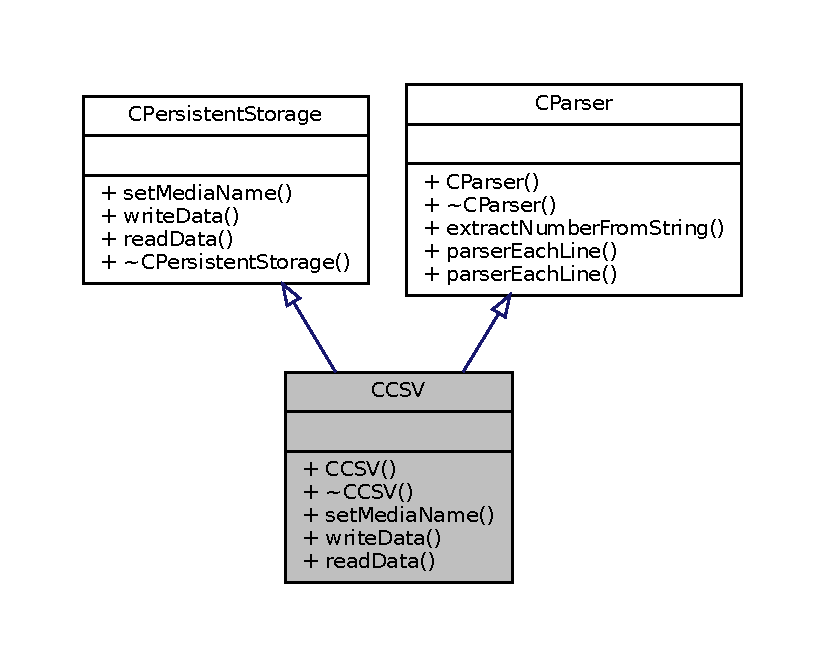
\includegraphics[width=350pt]{classCCSV__inherit__graph}
\end{center}
\end{figure}


Collaboration diagram for C\+C\+SV\+:
\nopagebreak
\begin{figure}[H]
\begin{center}
\leavevmode
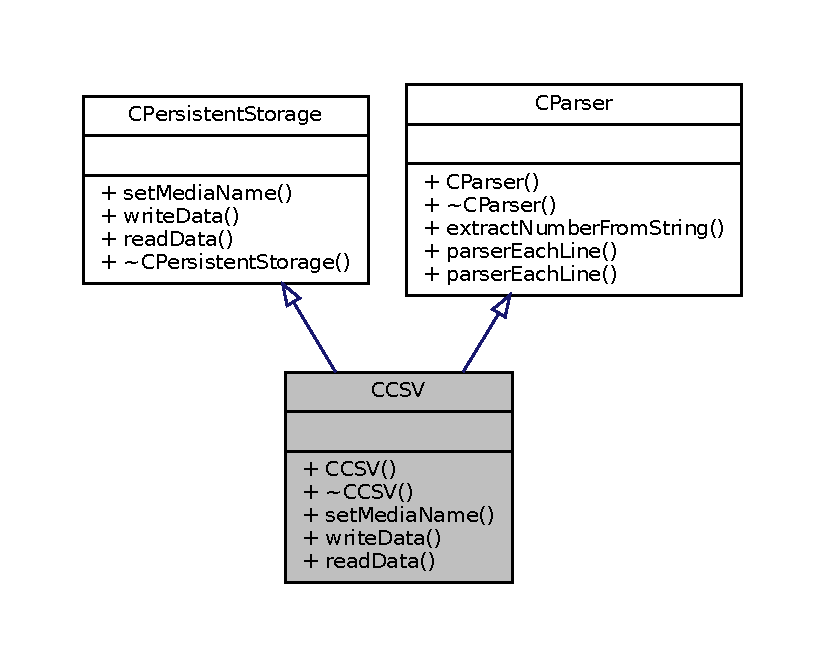
\includegraphics[width=350pt]{classCCSV__coll__graph}
\end{center}
\end{figure}
\subsection*{Public Member Functions}
\begin{DoxyCompactItemize}
\item 
\hyperlink{classCCSV_af643bffe19b07da7ecad5c4a6cfd82c0}{C\+C\+SV} ()
\item 
\hyperlink{classCCSV_aa1a56cc8993767e5f0572b839c594bec}{$\sim$\+C\+C\+SV} ()
\item 
void \hyperlink{classCCSV_a473f20a4cb83f3f50174a194121138d1}{set\+Media\+Name} (std\+::string name)
\item 
bool \hyperlink{classCCSV_a9f0f855c4337078ab3ccff7a3a8148fa}{write\+Data} (const \hyperlink{classCWpDatabase}{C\+Wp\+Database} \&waypoint\+Db, const \hyperlink{classCPoiDatabase}{C\+Poi\+Database} \&poi\+Db)
\item 
bool \hyperlink{classCCSV_a861ad5d158b00a1eaef4d45710aa466c}{read\+Data} (\hyperlink{classCWpDatabase}{C\+Wp\+Database} \&waypoint\+Db, \hyperlink{classCPoiDatabase}{C\+Poi\+Database} \&poi\+Db, \hyperlink{classCPersistentStorage_a9b9929a4afa6e21da10f4a2e926a4584}{Merge\+Mode} mode)
\end{DoxyCompactItemize}
\subsection*{Additional Inherited Members}


\subsection{Constructor \& Destructor Documentation}
\mbox{\Hypertarget{classCCSV_af643bffe19b07da7ecad5c4a6cfd82c0}\label{classCCSV_af643bffe19b07da7ecad5c4a6cfd82c0}} 
\index{C\+C\+SV@{C\+C\+SV}!C\+C\+SV@{C\+C\+SV}}
\index{C\+C\+SV@{C\+C\+SV}!C\+C\+SV@{C\+C\+SV}}
\subsubsection{\texorpdfstring{C\+C\+S\+V()}{CCSV()}}
{\footnotesize\ttfamily C\+C\+S\+V\+::\+C\+C\+SV (\begin{DoxyParamCaption}{ }\end{DoxyParamCaption})}

Constructor \mbox{\Hypertarget{classCCSV_aa1a56cc8993767e5f0572b839c594bec}\label{classCCSV_aa1a56cc8993767e5f0572b839c594bec}} 
\index{C\+C\+SV@{C\+C\+SV}!````~C\+C\+SV@{$\sim$\+C\+C\+SV}}
\index{````~C\+C\+SV@{$\sim$\+C\+C\+SV}!C\+C\+SV@{C\+C\+SV}}
\subsubsection{\texorpdfstring{$\sim$\+C\+C\+S\+V()}{~CCSV()}}
{\footnotesize\ttfamily C\+C\+S\+V\+::$\sim$\+C\+C\+SV (\begin{DoxyParamCaption}{ }\end{DoxyParamCaption})}

Destructor 

\subsection{Member Function Documentation}
\mbox{\Hypertarget{classCCSV_a861ad5d158b00a1eaef4d45710aa466c}\label{classCCSV_a861ad5d158b00a1eaef4d45710aa466c}} 
\index{C\+C\+SV@{C\+C\+SV}!read\+Data@{read\+Data}}
\index{read\+Data@{read\+Data}!C\+C\+SV@{C\+C\+SV}}
\subsubsection{\texorpdfstring{read\+Data()}{readData()}}
{\footnotesize\ttfamily bool C\+C\+S\+V\+::read\+Data (\begin{DoxyParamCaption}\item[{\hyperlink{classCWpDatabase}{C\+Wp\+Database} \&}]{waypoint\+Db,  }\item[{\hyperlink{classCPoiDatabase}{C\+Poi\+Database} \&}]{poi\+Db,  }\item[{\hyperlink{classCPersistentStorage_a9b9929a4afa6e21da10f4a2e926a4584}{Merge\+Mode}}]{mode }\end{DoxyParamCaption})\hspace{0.3cm}{\ttfamily [virtual]}}

Fill the databases with the data from persistent storage. If merge mode is M\+E\+R\+GE, the content in the persistent storage will be merged with any content already existing in the data bases. If merge mode is R\+E\+P\+L\+A\+CE, already existing content will be removed before inserting the content from the persistent storage.


\begin{DoxyParams}{Parameters}
{\em waypoint\+Db} & the the data base with way points \\
\hline
{\em poi\+Db} & the database with points of interest \\
\hline
{\em mode} & the merge mode \\
\hline
\end{DoxyParams}
\begin{DoxyReturn}{Returns}
true if the data could be read successfully 
\end{DoxyReturn}


Implements \hyperlink{classCPersistentStorage_a28edf547e10449a7f45de9885b68890b}{C\+Persistent\+Storage}.

\mbox{\Hypertarget{classCCSV_a473f20a4cb83f3f50174a194121138d1}\label{classCCSV_a473f20a4cb83f3f50174a194121138d1}} 
\index{C\+C\+SV@{C\+C\+SV}!set\+Media\+Name@{set\+Media\+Name}}
\index{set\+Media\+Name@{set\+Media\+Name}!C\+C\+SV@{C\+C\+SV}}
\subsubsection{\texorpdfstring{set\+Media\+Name()}{setMediaName()}}
{\footnotesize\ttfamily void C\+C\+S\+V\+::set\+Media\+Name (\begin{DoxyParamCaption}\item[{std\+::string}]{name }\end{DoxyParamCaption})\hspace{0.3cm}{\ttfamily [virtual]}}

Set the name of the media to be used for persistent storage. The exact interpretation of the name depends on the implementation of the component.


\begin{DoxyParams}{Parameters}
{\em name} & the media to be used  void \\
\hline
\end{DoxyParams}


Implements \hyperlink{classCPersistentStorage_af626d001915346c04c2008c9ea8bb8d8}{C\+Persistent\+Storage}.

\mbox{\Hypertarget{classCCSV_a9f0f855c4337078ab3ccff7a3a8148fa}\label{classCCSV_a9f0f855c4337078ab3ccff7a3a8148fa}} 
\index{C\+C\+SV@{C\+C\+SV}!write\+Data@{write\+Data}}
\index{write\+Data@{write\+Data}!C\+C\+SV@{C\+C\+SV}}
\subsubsection{\texorpdfstring{write\+Data()}{writeData()}}
{\footnotesize\ttfamily bool C\+C\+S\+V\+::write\+Data (\begin{DoxyParamCaption}\item[{const \hyperlink{classCWpDatabase}{C\+Wp\+Database} \&}]{waypoint\+Db,  }\item[{const \hyperlink{classCPoiDatabase}{C\+Poi\+Database} \&}]{poi\+Db }\end{DoxyParamCaption})\hspace{0.3cm}{\ttfamily [virtual]}}

Write the data to the persistent storage.


\begin{DoxyParams}{Parameters}
{\em waypoint\+Db} & the data base with way points \\
\hline
{\em poi\+Db} & the database with points of interest \\
\hline
\end{DoxyParams}
\begin{DoxyReturn}{Returns}
true if the data could be saved successfully 
\end{DoxyReturn}


Implements \hyperlink{classCPersistentStorage_ab0c03dbf674c6218d574289ec54a75ed}{C\+Persistent\+Storage}.



The documentation for this class was generated from the following files\+:\begin{DoxyCompactItemize}
\item 
\hyperlink{CCSV_8h}{C\+C\+S\+V.\+h}\item 
\hyperlink{CCSV_8cpp}{C\+C\+S\+V.\+cpp}\end{DoxyCompactItemize}

\hypertarget{classCDatabase}{}\section{C\+Database$<$ T1, T2 $>$ Class Template Reference}
\label{classCDatabase}\index{C\+Database$<$ T1, T2 $>$@{C\+Database$<$ T1, T2 $>$}}


{\ttfamily \#include $<$C\+Database.\+h$>$}



Collaboration diagram for C\+Database$<$ T1, T2 $>$\+:
\nopagebreak
\begin{figure}[H]
\begin{center}
\leavevmode
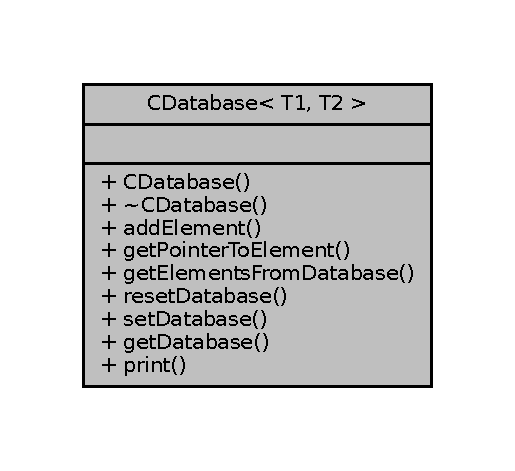
\includegraphics[width=247pt]{classCDatabase__coll__graph}
\end{center}
\end{figure}
\subsection*{Public Types}
\begin{DoxyCompactItemize}
\item 
typedef std\+::map$<$ T1, T2 $>$ \hyperlink{classCDatabase_ac20411b7c5997877aebb46d0bd3a8461}{Database\+\_\+\+Container\+\_\+t}
\item 
typedef std\+::map$<$ T1, T2 $>$\+::iterator \hyperlink{classCDatabase_a07aa3db528b07931347d91ebf505b8ed}{Database\+\_\+\+Container\+\_\+\+Itr\+\_\+t}
\item 
typedef T1 \hyperlink{classCDatabase_aa48e663caabc489e9aa738e299d10ee0}{Database\+\_\+\+Container\+\_\+key\+\_\+t}
\end{DoxyCompactItemize}
\subsection*{Public Member Functions}
\begin{DoxyCompactItemize}
\item 
\hyperlink{classCDatabase_ac5fd82bb19a12e500d2f65cbd919c256}{C\+Database} ()
\item 
\hyperlink{classCDatabase_a2b3592b975d43dfb06e4bac2a4245c7b}{$\sim$\+C\+Database} ()
\item 
void \hyperlink{classCDatabase_a269a0a23ba838e0c6ce533017a0d635a}{add\+Element} (T1 const \&key, T2 const \&elem)
\item 
T2 $\ast$ \hyperlink{classCDatabase_a708130facbed33fd15956bf3cf760372}{get\+Pointer\+To\+Element} (T1 elem\+Identifier)
\item 
const \hyperlink{classCDatabase_ac20411b7c5997877aebb46d0bd3a8461}{Database\+\_\+\+Container\+\_\+t} \hyperlink{classCDatabase_a2ecfd5ba202cea2332ddcd59237baf8e}{get\+Elements\+From\+Database} () const
\item 
void \hyperlink{classCDatabase_a96f398964530b48ad7fc63c05783369f}{reset\+Database} ()
\item 
void \hyperlink{classCDatabase_a695c6bbbf0fc27a07cd520a5eda81128}{set\+Database} (\hyperlink{classCDatabase_ac20411b7c5997877aebb46d0bd3a8461}{Database\+\_\+\+Container\+\_\+t} const elems\+Eontainer)
\item 
\hyperlink{classCDatabase_ac20411b7c5997877aebb46d0bd3a8461}{Database\+\_\+\+Container\+\_\+t} const \hyperlink{classCDatabase_a7991d341e324528af43b4a1a2a09f39f}{get\+Database} ()
\item 
void \hyperlink{classCDatabase_aeaff36fd440603cb8308676c7e4eb296}{print} ()
\end{DoxyCompactItemize}


\subsection{Member Typedef Documentation}
\mbox{\Hypertarget{classCDatabase_a07aa3db528b07931347d91ebf505b8ed}\label{classCDatabase_a07aa3db528b07931347d91ebf505b8ed}} 
\index{C\+Database@{C\+Database}!Database\+\_\+\+Container\+\_\+\+Itr\+\_\+t@{Database\+\_\+\+Container\+\_\+\+Itr\+\_\+t}}
\index{Database\+\_\+\+Container\+\_\+\+Itr\+\_\+t@{Database\+\_\+\+Container\+\_\+\+Itr\+\_\+t}!C\+Database@{C\+Database}}
\subsubsection{\texorpdfstring{Database\+\_\+\+Container\+\_\+\+Itr\+\_\+t}{Database\_Container\_Itr\_t}}
{\footnotesize\ttfamily template$<$class T1, class T2$>$ \\
typedef std\+::map$<$T1, T2$>$\+::iterator \hyperlink{classCDatabase}{C\+Database}$<$ T1, T2 $>$\+::\hyperlink{classCDatabase_a07aa3db528b07931347d91ebf505b8ed}{Database\+\_\+\+Container\+\_\+\+Itr\+\_\+t}}

\mbox{\Hypertarget{classCDatabase_aa48e663caabc489e9aa738e299d10ee0}\label{classCDatabase_aa48e663caabc489e9aa738e299d10ee0}} 
\index{C\+Database@{C\+Database}!Database\+\_\+\+Container\+\_\+key\+\_\+t@{Database\+\_\+\+Container\+\_\+key\+\_\+t}}
\index{Database\+\_\+\+Container\+\_\+key\+\_\+t@{Database\+\_\+\+Container\+\_\+key\+\_\+t}!C\+Database@{C\+Database}}
\subsubsection{\texorpdfstring{Database\+\_\+\+Container\+\_\+key\+\_\+t}{Database\_Container\_key\_t}}
{\footnotesize\ttfamily template$<$class T1, class T2$>$ \\
typedef T1 \hyperlink{classCDatabase}{C\+Database}$<$ T1, T2 $>$\+::\hyperlink{classCDatabase_aa48e663caabc489e9aa738e299d10ee0}{Database\+\_\+\+Container\+\_\+key\+\_\+t}}

\mbox{\Hypertarget{classCDatabase_ac20411b7c5997877aebb46d0bd3a8461}\label{classCDatabase_ac20411b7c5997877aebb46d0bd3a8461}} 
\index{C\+Database@{C\+Database}!Database\+\_\+\+Container\+\_\+t@{Database\+\_\+\+Container\+\_\+t}}
\index{Database\+\_\+\+Container\+\_\+t@{Database\+\_\+\+Container\+\_\+t}!C\+Database@{C\+Database}}
\subsubsection{\texorpdfstring{Database\+\_\+\+Container\+\_\+t}{Database\_Container\_t}}
{\footnotesize\ttfamily template$<$class T1, class T2$>$ \\
typedef std\+::map$<$T1, T2$>$ \hyperlink{classCDatabase}{C\+Database}$<$ T1, T2 $>$\+::\hyperlink{classCDatabase_ac20411b7c5997877aebb46d0bd3a8461}{Database\+\_\+\+Container\+\_\+t}}



\subsection{Constructor \& Destructor Documentation}
\mbox{\Hypertarget{classCDatabase_ac5fd82bb19a12e500d2f65cbd919c256}\label{classCDatabase_ac5fd82bb19a12e500d2f65cbd919c256}} 
\index{C\+Database@{C\+Database}!C\+Database@{C\+Database}}
\index{C\+Database@{C\+Database}!C\+Database@{C\+Database}}
\subsubsection{\texorpdfstring{C\+Database()}{CDatabase()}}
{\footnotesize\ttfamily template$<$class T1 , class T2 $>$ \\
\hyperlink{classCDatabase}{C\+Database}$<$ T1, T2 $>$\+::\hyperlink{classCDatabase}{C\+Database} (\begin{DoxyParamCaption}{ }\end{DoxyParamCaption})}

\hyperlink{classCDatabase}{C\+Database} constructor \mbox{\Hypertarget{classCDatabase_a2b3592b975d43dfb06e4bac2a4245c7b}\label{classCDatabase_a2b3592b975d43dfb06e4bac2a4245c7b}} 
\index{C\+Database@{C\+Database}!````~C\+Database@{$\sim$\+C\+Database}}
\index{````~C\+Database@{$\sim$\+C\+Database}!C\+Database@{C\+Database}}
\subsubsection{\texorpdfstring{$\sim$\+C\+Database()}{~CDatabase()}}
{\footnotesize\ttfamily template$<$class T1 , class T2 $>$ \\
\hyperlink{classCDatabase}{C\+Database}$<$ T1, T2 $>$\+::$\sim$\hyperlink{classCDatabase}{C\+Database} (\begin{DoxyParamCaption}{ }\end{DoxyParamCaption})}

\hyperlink{classCDatabase}{C\+Database} destructor 

\subsection{Member Function Documentation}
\mbox{\Hypertarget{classCDatabase_a269a0a23ba838e0c6ce533017a0d635a}\label{classCDatabase_a269a0a23ba838e0c6ce533017a0d635a}} 
\index{C\+Database@{C\+Database}!add\+Element@{add\+Element}}
\index{add\+Element@{add\+Element}!C\+Database@{C\+Database}}
\subsubsection{\texorpdfstring{add\+Element()}{addElement()}}
{\footnotesize\ttfamily template$<$class T1, class T2$>$ \\
void \hyperlink{classCDatabase}{C\+Database}$<$ T1, T2 $>$\+::add\+Element (\begin{DoxyParamCaption}\item[{T1 const \&}]{key,  }\item[{T2 const \&}]{elem }\end{DoxyParamCaption})}

Add an element to the database param@ T1 const \&key -\/ a key to associative container (IN) param@ T2 const \&elem -\/ an element to be added (IN) returnvalue@ void \mbox{\Hypertarget{classCDatabase_a7991d341e324528af43b4a1a2a09f39f}\label{classCDatabase_a7991d341e324528af43b4a1a2a09f39f}} 
\index{C\+Database@{C\+Database}!get\+Database@{get\+Database}}
\index{get\+Database@{get\+Database}!C\+Database@{C\+Database}}
\subsubsection{\texorpdfstring{get\+Database()}{getDatabase()}}
{\footnotesize\ttfamily template$<$class T1 , class T2 $>$ \\
const \hyperlink{classCDatabase}{C\+Database}$<$ T1, T2 $>$\+::\hyperlink{classCDatabase_ac20411b7c5997877aebb46d0bd3a8461}{Database\+\_\+\+Container\+\_\+t} \hyperlink{classCDatabase}{C\+Database}$<$ T1, T2 $>$\+::get\+Database (\begin{DoxyParamCaption}{ }\end{DoxyParamCaption})}

Getter method Database returnvalue@ Database\+\_\+\+Container\+\_\+t const \mbox{\Hypertarget{classCDatabase_a2ecfd5ba202cea2332ddcd59237baf8e}\label{classCDatabase_a2ecfd5ba202cea2332ddcd59237baf8e}} 
\index{C\+Database@{C\+Database}!get\+Elements\+From\+Database@{get\+Elements\+From\+Database}}
\index{get\+Elements\+From\+Database@{get\+Elements\+From\+Database}!C\+Database@{C\+Database}}
\subsubsection{\texorpdfstring{get\+Elements\+From\+Database()}{getElementsFromDatabase()}}
{\footnotesize\ttfamily template$<$class T1 , class T2 $>$ \\
const \hyperlink{classCDatabase}{C\+Database}$<$ T1, T2 $>$\+::\hyperlink{classCDatabase_ac20411b7c5997877aebb46d0bd3a8461}{Database\+\_\+\+Container\+\_\+t} \hyperlink{classCDatabase}{C\+Database}$<$ T1, T2 $>$\+::get\+Elements\+From\+Database (\begin{DoxyParamCaption}{ }\end{DoxyParamCaption}) const}

Get Elements\textquotesingle{} container from the Database returnvalue@ Database\+\_\+\+Container\+\_\+t -\/ Elements in the Database (O\+UT) \mbox{\Hypertarget{classCDatabase_a708130facbed33fd15956bf3cf760372}\label{classCDatabase_a708130facbed33fd15956bf3cf760372}} 
\index{C\+Database@{C\+Database}!get\+Pointer\+To\+Element@{get\+Pointer\+To\+Element}}
\index{get\+Pointer\+To\+Element@{get\+Pointer\+To\+Element}!C\+Database@{C\+Database}}
\subsubsection{\texorpdfstring{get\+Pointer\+To\+Element()}{getPointerToElement()}}
{\footnotesize\ttfamily template$<$class T1, class T2 $>$ \\
T2 $\ast$ \hyperlink{classCDatabase}{C\+Database}$<$ T1, T2 $>$\+::get\+Pointer\+To\+Element (\begin{DoxyParamCaption}\item[{T1}]{elem\+Identifier }\end{DoxyParamCaption})}

Get pointer to an element from the Database which matches the key param@ T1 elem\+Identifier -\/ Identifier for an element (IN) returnvalue@ T2$\ast$ -\/ Pointer to the element in the database \mbox{\Hypertarget{classCDatabase_aeaff36fd440603cb8308676c7e4eb296}\label{classCDatabase_aeaff36fd440603cb8308676c7e4eb296}} 
\index{C\+Database@{C\+Database}!print@{print}}
\index{print@{print}!C\+Database@{C\+Database}}
\subsubsection{\texorpdfstring{print()}{print()}}
{\footnotesize\ttfamily template$<$class T1 , class T2 $>$ \\
void \hyperlink{classCDatabase}{C\+Database}$<$ T1, T2 $>$\+::print (\begin{DoxyParamCaption}{ }\end{DoxyParamCaption})}

Print all the elements in the database returnvalue@ void \mbox{\Hypertarget{classCDatabase_a96f398964530b48ad7fc63c05783369f}\label{classCDatabase_a96f398964530b48ad7fc63c05783369f}} 
\index{C\+Database@{C\+Database}!reset\+Database@{reset\+Database}}
\index{reset\+Database@{reset\+Database}!C\+Database@{C\+Database}}
\subsubsection{\texorpdfstring{reset\+Database()}{resetDatabase()}}
{\footnotesize\ttfamily template$<$class T1 , class T2 $>$ \\
void \hyperlink{classCDatabase}{C\+Database}$<$ T1, T2 $>$\+::reset\+Database (\begin{DoxyParamCaption}{ }\end{DoxyParamCaption})}

Resets the Database returnvalue@ void \mbox{\Hypertarget{classCDatabase_a695c6bbbf0fc27a07cd520a5eda81128}\label{classCDatabase_a695c6bbbf0fc27a07cd520a5eda81128}} 
\index{C\+Database@{C\+Database}!set\+Database@{set\+Database}}
\index{set\+Database@{set\+Database}!C\+Database@{C\+Database}}
\subsubsection{\texorpdfstring{set\+Database()}{setDatabase()}}
{\footnotesize\ttfamily template$<$class T1 , class T2 $>$ \\
void \hyperlink{classCDatabase}{C\+Database}$<$ T1, T2 $>$\+::set\+Database (\begin{DoxyParamCaption}\item[{\hyperlink{classCDatabase_ac20411b7c5997877aebb46d0bd3a8461}{Database\+\_\+\+Container\+\_\+t} const}]{elems\+Eontainer }\end{DoxyParamCaption})}

Setter method Database param@ Database\+\_\+\+Container\+\_\+t const elems\+Eontainer returnvalue@ void

Setter method Database returnvalue@ void 

The documentation for this class was generated from the following file\+:\begin{DoxyCompactItemize}
\item 
\hyperlink{CDatabase_8h}{C\+Database.\+h}\end{DoxyCompactItemize}

\hypertarget{classCGPSSensor}{}\section{C\+G\+P\+S\+Sensor Class Reference}
\label{classCGPSSensor}\index{C\+G\+P\+S\+Sensor@{C\+G\+P\+S\+Sensor}}


{\ttfamily \#include $<$C\+G\+P\+S\+Sensor.\+h$>$}



Collaboration diagram for C\+G\+P\+S\+Sensor\+:
\nopagebreak
\begin{figure}[H]
\begin{center}
\leavevmode
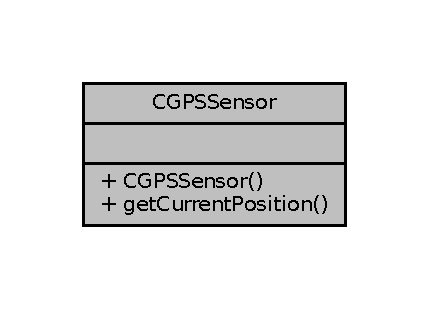
\includegraphics[width=206pt]{classCGPSSensor__coll__graph}
\end{center}
\end{figure}
\subsection*{Public Member Functions}
\begin{DoxyCompactItemize}
\item 
\hyperlink{classCGPSSensor_ab9d50cfdb88349ca752423cc6f6796ef}{C\+G\+P\+S\+Sensor} ()
\item 
\hyperlink{classCWaypoint}{C\+Waypoint} \hyperlink{classCGPSSensor_a6a3f3e3070e5f0c566712ea62b652684}{get\+Current\+Position} ()
\end{DoxyCompactItemize}


\subsection{Constructor \& Destructor Documentation}
\mbox{\Hypertarget{classCGPSSensor_ab9d50cfdb88349ca752423cc6f6796ef}\label{classCGPSSensor_ab9d50cfdb88349ca752423cc6f6796ef}} 
\index{C\+G\+P\+S\+Sensor@{C\+G\+P\+S\+Sensor}!C\+G\+P\+S\+Sensor@{C\+G\+P\+S\+Sensor}}
\index{C\+G\+P\+S\+Sensor@{C\+G\+P\+S\+Sensor}!C\+G\+P\+S\+Sensor@{C\+G\+P\+S\+Sensor}}
\subsubsection{\texorpdfstring{C\+G\+P\+S\+Sensor()}{CGPSSensor()}}
{\footnotesize\ttfamily C\+G\+P\+S\+Sensor\+::\+C\+G\+P\+S\+Sensor (\begin{DoxyParamCaption}{ }\end{DoxyParamCaption})}

\hyperlink{classCGPSSensor}{C\+G\+P\+S\+Sensor} constructor 

\subsection{Member Function Documentation}
\mbox{\Hypertarget{classCGPSSensor_a6a3f3e3070e5f0c566712ea62b652684}\label{classCGPSSensor_a6a3f3e3070e5f0c566712ea62b652684}} 
\index{C\+G\+P\+S\+Sensor@{C\+G\+P\+S\+Sensor}!get\+Current\+Position@{get\+Current\+Position}}
\index{get\+Current\+Position@{get\+Current\+Position}!C\+G\+P\+S\+Sensor@{C\+G\+P\+S\+Sensor}}
\subsubsection{\texorpdfstring{get\+Current\+Position()}{getCurrentPosition()}}
{\footnotesize\ttfamily \hyperlink{classCWaypoint}{C\+Waypoint} C\+G\+P\+S\+Sensor\+::get\+Current\+Position (\begin{DoxyParamCaption}{ }\end{DoxyParamCaption})}

Get the current position from the sensor  \hyperlink{classCWaypoint}{C\+Waypoint} 

The documentation for this class was generated from the following files\+:\begin{DoxyCompactItemize}
\item 
\hyperlink{CGPSSensor_8h}{C\+G\+P\+S\+Sensor.\+h}\item 
\hyperlink{CGPSSensor_8cpp}{C\+G\+P\+S\+Sensor.\+cpp}\end{DoxyCompactItemize}

\hypertarget{classCJsonPersistence}{}\section{C\+Json\+Persistence Class Reference}
\label{classCJsonPersistence}\index{C\+Json\+Persistence@{C\+Json\+Persistence}}


{\ttfamily \#include $<$C\+Json\+Persistence.\+h$>$}



Inheritance diagram for C\+Json\+Persistence\+:
\nopagebreak
\begin{figure}[H]
\begin{center}
\leavevmode
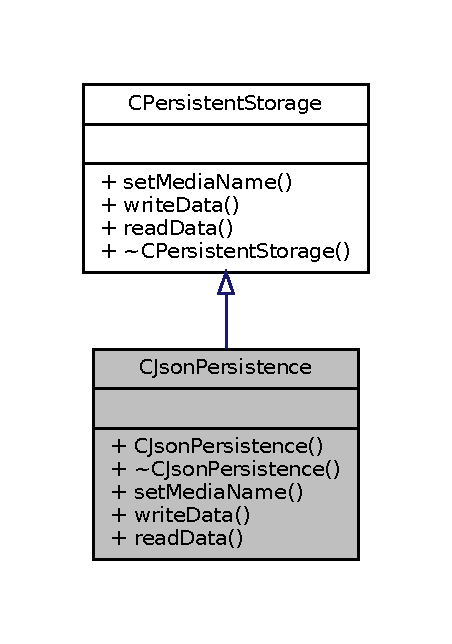
\includegraphics[width=217pt]{classCJsonPersistence__inherit__graph}
\end{center}
\end{figure}


Collaboration diagram for C\+Json\+Persistence\+:
\nopagebreak
\begin{figure}[H]
\begin{center}
\leavevmode
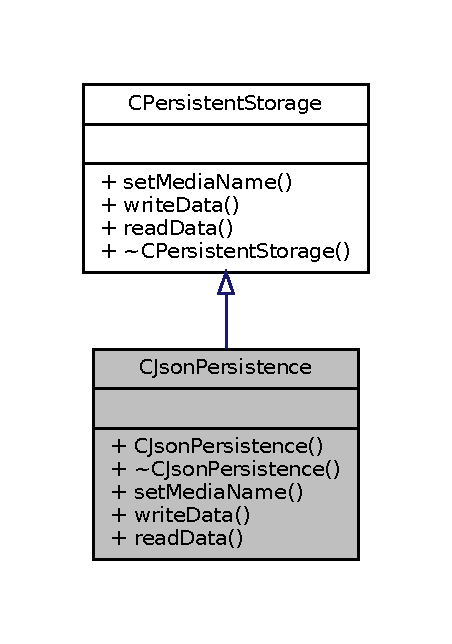
\includegraphics[width=217pt]{classCJsonPersistence__coll__graph}
\end{center}
\end{figure}
\subsection*{Public Types}
\begin{DoxyCompactItemize}
\item 
enum \hyperlink{classCJsonPersistence_a32c7998a8554b336a0d7f44e10686525}{json\+Objects} \{ \hyperlink{classCJsonPersistence_a32c7998a8554b336a0d7f44e10686525a963baef36cfee6c583e0033b120fb21e}{W\+A\+Y\+P\+O\+I\+N\+TS} = 0, 
\hyperlink{classCJsonPersistence_a32c7998a8554b336a0d7f44e10686525a4033b9ccdf12ae4e1eab1e985d90d1a4}{P\+O\+I\+N\+T\+\_\+\+O\+F\+\_\+\+I\+N\+T\+E\+R\+E\+ST}, 
\hyperlink{classCJsonPersistence_a32c7998a8554b336a0d7f44e10686525a53031fa62b5180ac9feffd460aa23b61}{M\+A\+X\+\_\+\+J\+S\+O\+N\+\_\+\+O\+B\+J\+E\+C\+TS}
 \}
\item 
enum \hyperlink{classCJsonPersistence_a51707f5742e8804c7c17495791da674c}{read\+States} \{ \newline
\hyperlink{classCJsonPersistence_a51707f5742e8804c7c17495791da674cad4f6e6d5bb4ff97b9cc6466e9d58d4d7}{W\+A\+I\+T\+I\+N\+G\+\_\+\+F\+O\+R\+\_\+\+B\+E\+G\+I\+N\+\_\+\+O\+B\+J\+E\+CT}, 
\hyperlink{classCJsonPersistence_a51707f5742e8804c7c17495791da674ca8c55dd61dcaed312b81f0f648c54879e}{W\+A\+I\+T\+I\+N\+G\+\_\+\+F\+O\+R\+\_\+\+D\+B\+\_\+\+N\+A\+ME}, 
\hyperlink{classCJsonPersistence_a51707f5742e8804c7c17495791da674cac61f2d6dd3c0203b2458e83f7a5a1435}{W\+A\+I\+T\+I\+N\+G\+\_\+\+F\+O\+R\+\_\+\+D\+B\+\_\+\+A\+R\+R\+A\+Y\+\_\+\+B\+E\+G\+IN}, 
\hyperlink{classCJsonPersistence_a51707f5742e8804c7c17495791da674ca7a5b17132dd7fd839ab80473d262fc62}{W\+A\+I\+T\+I\+N\+G\+\_\+\+F\+O\+R\+\_\+\+D\+B\+\_\+\+O\+B\+J\+E\+C\+T\+\_\+\+B\+E\+G\+IN}, 
\newline
\hyperlink{classCJsonPersistence_a51707f5742e8804c7c17495791da674caa0c6b41380f8137cdb65fb4925dd12ba}{W\+A\+I\+T\+I\+N\+G\+\_\+\+F\+O\+R\+\_\+\+D\+B\+\_\+\+O\+B\+J\+E\+C\+T\+\_\+\+E\+ND}, 
\hyperlink{classCJsonPersistence_a51707f5742e8804c7c17495791da674cadb84feef04d47a48ddd0232c8c96d5fe}{W\+A\+I\+T\+I\+N\+G\+\_\+\+F\+O\+R\+\_\+\+A\+T\+T\+R\+I\+B\+U\+T\+E\+\_\+\+N\+A\+ME}, 
\hyperlink{classCJsonPersistence_a51707f5742e8804c7c17495791da674caa4a6e877d4f719757cae30457217a24d}{W\+A\+I\+T\+I\+N\+G\+\_\+\+F\+O\+R\+\_\+\+N\+A\+M\+E\+\_\+\+S\+E\+P\+A\+R\+A\+T\+OR}, 
\hyperlink{classCJsonPersistence_a51707f5742e8804c7c17495791da674cab6451c0867f3f950fc867d8e1e6f6c42}{W\+A\+I\+T\+I\+N\+G\+\_\+\+F\+O\+R\+\_\+\+V\+A\+L\+UE}, 
\newline
\hyperlink{classCJsonPersistence_a51707f5742e8804c7c17495791da674cab812c6537b104b4b9c738bc9f067af79}{W\+A\+I\+T\+I\+N\+G\+\_\+\+F\+O\+R\+\_\+\+V\+A\+L\+U\+E\+\_\+\+S\+E\+P\+A\+R\+A\+T\+OR}, 
\hyperlink{classCJsonPersistence_a51707f5742e8804c7c17495791da674cac2e24e77b09d77dc505b15449a8577e8}{W\+A\+I\+T\+I\+N\+G\+\_\+\+F\+O\+R\+\_\+\+C\+O\+M\+P\+L\+E\+T\+I\+ON}
 \}
\item 
enum \hyperlink{classCJsonPersistence_a14ff5edefd4a4aac6fb0559cfbf4b7fa}{json\+Read\+Exceptions} \{ \newline
\hyperlink{classCJsonPersistence_a14ff5edefd4a4aac6fb0559cfbf4b7faa14e442c1343ab3ac8fdcd2b7c696aede}{J\+S\+O\+N\+\_\+\+E\+R\+R\+\_\+\+NO} = -\/1, 
\hyperlink{classCJsonPersistence_a14ff5edefd4a4aac6fb0559cfbf4b7faa2122f517c76588a93b17b30dfc86f38e}{J\+S\+O\+N\+\_\+\+E\+R\+R\+\_\+\+E\+X\+P\+E\+C\+T\+\_\+\+B\+E\+G\+I\+N\+\_\+\+O\+B\+J\+E\+CT}, 
\hyperlink{classCJsonPersistence_a14ff5edefd4a4aac6fb0559cfbf4b7faa082a9d09bf852aa55521f21071626d5c}{J\+S\+O\+N\+\_\+\+E\+R\+R\+\_\+\+E\+X\+P\+E\+C\+T\+\_\+\+D\+B\+\_\+\+N\+A\+M\+E\+\_\+\+S\+T\+R\+I\+NG}, 
\hyperlink{classCJsonPersistence_a14ff5edefd4a4aac6fb0559cfbf4b7faa08e44398e606d09d2043fce4d6e2cf1d}{J\+S\+O\+N\+\_\+\+E\+R\+R\+\_\+\+E\+X\+P\+E\+C\+T\+\_\+\+N\+A\+M\+E\+\_\+\+S\+E\+P\+A\+R\+A\+T\+OR}, 
\newline
\hyperlink{classCJsonPersistence_a14ff5edefd4a4aac6fb0559cfbf4b7faa2597b46f8ae18cfc77b402f7e2112230}{J\+S\+O\+N\+\_\+\+E\+R\+R\+\_\+\+E\+X\+P\+E\+C\+T\+\_\+\+D\+B\+\_\+\+A\+R\+R\+A\+Y\+\_\+\+B\+E\+G\+IN}, 
\hyperlink{classCJsonPersistence_a14ff5edefd4a4aac6fb0559cfbf4b7faa1eb8b803408cbb855acb793ef5e24df1}{J\+S\+O\+N\+\_\+\+E\+R\+R\+\_\+\+E\+X\+P\+E\+C\+T\+\_\+\+D\+B\+\_\+\+O\+B\+J\+E\+C\+T\+\_\+\+B\+E\+G\+IN}, 
\hyperlink{classCJsonPersistence_a14ff5edefd4a4aac6fb0559cfbf4b7faa8872c69880179dcb420161dfde22dd84}{J\+S\+O\+N\+\_\+\+E\+R\+R\+\_\+\+E\+X\+P\+E\+C\+T\+\_\+\+D\+B\+\_\+\+O\+B\+J\+E\+C\+T\+\_\+\+E\+ND}, 
\hyperlink{classCJsonPersistence_a14ff5edefd4a4aac6fb0559cfbf4b7faa033e3643d78ac07295f5c26d9b6b913e}{J\+S\+O\+N\+\_\+\+E\+R\+R\+\_\+\+E\+X\+P\+E\+C\+T\+\_\+\+A\+T\+T\+R\+\_\+\+N\+A\+ME}, 
\newline
\hyperlink{classCJsonPersistence_a14ff5edefd4a4aac6fb0559cfbf4b7faa201f44a08d57f7af38042522c13b5d5b}{J\+S\+O\+N\+\_\+\+E\+R\+R\+\_\+\+E\+X\+P\+E\+C\+T\+\_\+\+A\+T\+T\+R\+\_\+\+V\+A\+L\+UE}, 
\hyperlink{classCJsonPersistence_a14ff5edefd4a4aac6fb0559cfbf4b7faa24b2dcf8d11a73e809ac11bb46701603}{J\+S\+O\+N\+\_\+\+E\+R\+R\+\_\+\+E\+X\+P\+E\+C\+T\+\_\+\+V\+A\+L\+U\+E\+\_\+\+S\+E\+P\+A\+R\+A\+T\+OR}, 
\hyperlink{classCJsonPersistence_a14ff5edefd4a4aac6fb0559cfbf4b7faaf2e3fbfd01567bac343e419211b4180f}{J\+S\+O\+N\+\_\+\+E\+R\+R\+\_\+\+I\+L\+L\+E\+G\+A\+L\+\_\+\+C\+H\+A\+R\+A\+C\+T\+ER}
 \}
\end{DoxyCompactItemize}
\subsection*{Public Member Functions}
\begin{DoxyCompactItemize}
\item 
\hyperlink{classCJsonPersistence_a4ecc6567fdd9d7f76ea3f53bbfd27a04}{C\+Json\+Persistence} ()
\item 
virtual \hyperlink{classCJsonPersistence_a4540b65d9b71826f3efa0342e9dc0f08}{$\sim$\+C\+Json\+Persistence} ()
\item 
void \hyperlink{classCJsonPersistence_a857d2c1a5de0f3fafceef1266e32a25d}{set\+Media\+Name} (std\+::string name)
\item 
bool \hyperlink{classCJsonPersistence_acd18e844bf7ec52ba1ec265ea2767dcb}{write\+Data} (const \hyperlink{classCWpDatabase}{C\+Wp\+Database} \&waypoint\+Db, const \hyperlink{classCPoiDatabase}{C\+Poi\+Database} \&poi\+Db)
\item 
bool \hyperlink{classCJsonPersistence_a433ddbf7f66175f38f549dbedcbb1e93}{read\+Data} (\hyperlink{classCWpDatabase}{C\+Wp\+Database} \&waypoint\+Db, \hyperlink{classCPoiDatabase}{C\+Poi\+Database} \&poi\+Db, \hyperlink{classCPersistentStorage_a9b9929a4afa6e21da10f4a2e926a4584}{Merge\+Mode} mode)
\end{DoxyCompactItemize}


\subsection{Member Enumeration Documentation}
\mbox{\Hypertarget{classCJsonPersistence_a32c7998a8554b336a0d7f44e10686525}\label{classCJsonPersistence_a32c7998a8554b336a0d7f44e10686525}} 
\index{C\+Json\+Persistence@{C\+Json\+Persistence}!json\+Objects@{json\+Objects}}
\index{json\+Objects@{json\+Objects}!C\+Json\+Persistence@{C\+Json\+Persistence}}
\subsubsection{\texorpdfstring{json\+Objects}{jsonObjects}}
{\footnotesize\ttfamily enum \hyperlink{classCJsonPersistence_a32c7998a8554b336a0d7f44e10686525}{C\+Json\+Persistence\+::json\+Objects}}

\begin{DoxyEnumFields}{Enumerator}
\raisebox{\heightof{T}}[0pt][0pt]{\index{W\+A\+Y\+P\+O\+I\+N\+TS@{W\+A\+Y\+P\+O\+I\+N\+TS}!C\+Json\+Persistence@{C\+Json\+Persistence}}\index{C\+Json\+Persistence@{C\+Json\+Persistence}!W\+A\+Y\+P\+O\+I\+N\+TS@{W\+A\+Y\+P\+O\+I\+N\+TS}}}\mbox{\Hypertarget{classCJsonPersistence_a32c7998a8554b336a0d7f44e10686525a963baef36cfee6c583e0033b120fb21e}\label{classCJsonPersistence_a32c7998a8554b336a0d7f44e10686525a963baef36cfee6c583e0033b120fb21e}} 
W\+A\+Y\+P\+O\+I\+N\+TS&\\
\hline

\raisebox{\heightof{T}}[0pt][0pt]{\index{P\+O\+I\+N\+T\+\_\+\+O\+F\+\_\+\+I\+N\+T\+E\+R\+E\+ST@{P\+O\+I\+N\+T\+\_\+\+O\+F\+\_\+\+I\+N\+T\+E\+R\+E\+ST}!C\+Json\+Persistence@{C\+Json\+Persistence}}\index{C\+Json\+Persistence@{C\+Json\+Persistence}!P\+O\+I\+N\+T\+\_\+\+O\+F\+\_\+\+I\+N\+T\+E\+R\+E\+ST@{P\+O\+I\+N\+T\+\_\+\+O\+F\+\_\+\+I\+N\+T\+E\+R\+E\+ST}}}\mbox{\Hypertarget{classCJsonPersistence_a32c7998a8554b336a0d7f44e10686525a4033b9ccdf12ae4e1eab1e985d90d1a4}\label{classCJsonPersistence_a32c7998a8554b336a0d7f44e10686525a4033b9ccdf12ae4e1eab1e985d90d1a4}} 
P\+O\+I\+N\+T\+\_\+\+O\+F\+\_\+\+I\+N\+T\+E\+R\+E\+ST&\\
\hline

\raisebox{\heightof{T}}[0pt][0pt]{\index{M\+A\+X\+\_\+\+J\+S\+O\+N\+\_\+\+O\+B\+J\+E\+C\+TS@{M\+A\+X\+\_\+\+J\+S\+O\+N\+\_\+\+O\+B\+J\+E\+C\+TS}!C\+Json\+Persistence@{C\+Json\+Persistence}}\index{C\+Json\+Persistence@{C\+Json\+Persistence}!M\+A\+X\+\_\+\+J\+S\+O\+N\+\_\+\+O\+B\+J\+E\+C\+TS@{M\+A\+X\+\_\+\+J\+S\+O\+N\+\_\+\+O\+B\+J\+E\+C\+TS}}}\mbox{\Hypertarget{classCJsonPersistence_a32c7998a8554b336a0d7f44e10686525a53031fa62b5180ac9feffd460aa23b61}\label{classCJsonPersistence_a32c7998a8554b336a0d7f44e10686525a53031fa62b5180ac9feffd460aa23b61}} 
M\+A\+X\+\_\+\+J\+S\+O\+N\+\_\+\+O\+B\+J\+E\+C\+TS&\\
\hline

\end{DoxyEnumFields}
\mbox{\Hypertarget{classCJsonPersistence_a14ff5edefd4a4aac6fb0559cfbf4b7fa}\label{classCJsonPersistence_a14ff5edefd4a4aac6fb0559cfbf4b7fa}} 
\index{C\+Json\+Persistence@{C\+Json\+Persistence}!json\+Read\+Exceptions@{json\+Read\+Exceptions}}
\index{json\+Read\+Exceptions@{json\+Read\+Exceptions}!C\+Json\+Persistence@{C\+Json\+Persistence}}
\subsubsection{\texorpdfstring{json\+Read\+Exceptions}{jsonReadExceptions}}
{\footnotesize\ttfamily enum \hyperlink{classCJsonPersistence_a14ff5edefd4a4aac6fb0559cfbf4b7fa}{C\+Json\+Persistence\+::json\+Read\+Exceptions}}

\begin{DoxyEnumFields}{Enumerator}
\raisebox{\heightof{T}}[0pt][0pt]{\index{J\+S\+O\+N\+\_\+\+E\+R\+R\+\_\+\+NO@{J\+S\+O\+N\+\_\+\+E\+R\+R\+\_\+\+NO}!C\+Json\+Persistence@{C\+Json\+Persistence}}\index{C\+Json\+Persistence@{C\+Json\+Persistence}!J\+S\+O\+N\+\_\+\+E\+R\+R\+\_\+\+NO@{J\+S\+O\+N\+\_\+\+E\+R\+R\+\_\+\+NO}}}\mbox{\Hypertarget{classCJsonPersistence_a14ff5edefd4a4aac6fb0559cfbf4b7faa14e442c1343ab3ac8fdcd2b7c696aede}\label{classCJsonPersistence_a14ff5edefd4a4aac6fb0559cfbf4b7faa14e442c1343ab3ac8fdcd2b7c696aede}} 
J\+S\+O\+N\+\_\+\+E\+R\+R\+\_\+\+NO&\\
\hline

\raisebox{\heightof{T}}[0pt][0pt]{\index{J\+S\+O\+N\+\_\+\+E\+R\+R\+\_\+\+E\+X\+P\+E\+C\+T\+\_\+\+B\+E\+G\+I\+N\+\_\+\+O\+B\+J\+E\+CT@{J\+S\+O\+N\+\_\+\+E\+R\+R\+\_\+\+E\+X\+P\+E\+C\+T\+\_\+\+B\+E\+G\+I\+N\+\_\+\+O\+B\+J\+E\+CT}!C\+Json\+Persistence@{C\+Json\+Persistence}}\index{C\+Json\+Persistence@{C\+Json\+Persistence}!J\+S\+O\+N\+\_\+\+E\+R\+R\+\_\+\+E\+X\+P\+E\+C\+T\+\_\+\+B\+E\+G\+I\+N\+\_\+\+O\+B\+J\+E\+CT@{J\+S\+O\+N\+\_\+\+E\+R\+R\+\_\+\+E\+X\+P\+E\+C\+T\+\_\+\+B\+E\+G\+I\+N\+\_\+\+O\+B\+J\+E\+CT}}}\mbox{\Hypertarget{classCJsonPersistence_a14ff5edefd4a4aac6fb0559cfbf4b7faa2122f517c76588a93b17b30dfc86f38e}\label{classCJsonPersistence_a14ff5edefd4a4aac6fb0559cfbf4b7faa2122f517c76588a93b17b30dfc86f38e}} 
J\+S\+O\+N\+\_\+\+E\+R\+R\+\_\+\+E\+X\+P\+E\+C\+T\+\_\+\+B\+E\+G\+I\+N\+\_\+\+O\+B\+J\+E\+CT&\\
\hline

\raisebox{\heightof{T}}[0pt][0pt]{\index{J\+S\+O\+N\+\_\+\+E\+R\+R\+\_\+\+E\+X\+P\+E\+C\+T\+\_\+\+D\+B\+\_\+\+N\+A\+M\+E\+\_\+\+S\+T\+R\+I\+NG@{J\+S\+O\+N\+\_\+\+E\+R\+R\+\_\+\+E\+X\+P\+E\+C\+T\+\_\+\+D\+B\+\_\+\+N\+A\+M\+E\+\_\+\+S\+T\+R\+I\+NG}!C\+Json\+Persistence@{C\+Json\+Persistence}}\index{C\+Json\+Persistence@{C\+Json\+Persistence}!J\+S\+O\+N\+\_\+\+E\+R\+R\+\_\+\+E\+X\+P\+E\+C\+T\+\_\+\+D\+B\+\_\+\+N\+A\+M\+E\+\_\+\+S\+T\+R\+I\+NG@{J\+S\+O\+N\+\_\+\+E\+R\+R\+\_\+\+E\+X\+P\+E\+C\+T\+\_\+\+D\+B\+\_\+\+N\+A\+M\+E\+\_\+\+S\+T\+R\+I\+NG}}}\mbox{\Hypertarget{classCJsonPersistence_a14ff5edefd4a4aac6fb0559cfbf4b7faa082a9d09bf852aa55521f21071626d5c}\label{classCJsonPersistence_a14ff5edefd4a4aac6fb0559cfbf4b7faa082a9d09bf852aa55521f21071626d5c}} 
J\+S\+O\+N\+\_\+\+E\+R\+R\+\_\+\+E\+X\+P\+E\+C\+T\+\_\+\+D\+B\+\_\+\+N\+A\+M\+E\+\_\+\+S\+T\+R\+I\+NG&\\
\hline

\raisebox{\heightof{T}}[0pt][0pt]{\index{J\+S\+O\+N\+\_\+\+E\+R\+R\+\_\+\+E\+X\+P\+E\+C\+T\+\_\+\+N\+A\+M\+E\+\_\+\+S\+E\+P\+A\+R\+A\+T\+OR@{J\+S\+O\+N\+\_\+\+E\+R\+R\+\_\+\+E\+X\+P\+E\+C\+T\+\_\+\+N\+A\+M\+E\+\_\+\+S\+E\+P\+A\+R\+A\+T\+OR}!C\+Json\+Persistence@{C\+Json\+Persistence}}\index{C\+Json\+Persistence@{C\+Json\+Persistence}!J\+S\+O\+N\+\_\+\+E\+R\+R\+\_\+\+E\+X\+P\+E\+C\+T\+\_\+\+N\+A\+M\+E\+\_\+\+S\+E\+P\+A\+R\+A\+T\+OR@{J\+S\+O\+N\+\_\+\+E\+R\+R\+\_\+\+E\+X\+P\+E\+C\+T\+\_\+\+N\+A\+M\+E\+\_\+\+S\+E\+P\+A\+R\+A\+T\+OR}}}\mbox{\Hypertarget{classCJsonPersistence_a14ff5edefd4a4aac6fb0559cfbf4b7faa08e44398e606d09d2043fce4d6e2cf1d}\label{classCJsonPersistence_a14ff5edefd4a4aac6fb0559cfbf4b7faa08e44398e606d09d2043fce4d6e2cf1d}} 
J\+S\+O\+N\+\_\+\+E\+R\+R\+\_\+\+E\+X\+P\+E\+C\+T\+\_\+\+N\+A\+M\+E\+\_\+\+S\+E\+P\+A\+R\+A\+T\+OR&\\
\hline

\raisebox{\heightof{T}}[0pt][0pt]{\index{J\+S\+O\+N\+\_\+\+E\+R\+R\+\_\+\+E\+X\+P\+E\+C\+T\+\_\+\+D\+B\+\_\+\+A\+R\+R\+A\+Y\+\_\+\+B\+E\+G\+IN@{J\+S\+O\+N\+\_\+\+E\+R\+R\+\_\+\+E\+X\+P\+E\+C\+T\+\_\+\+D\+B\+\_\+\+A\+R\+R\+A\+Y\+\_\+\+B\+E\+G\+IN}!C\+Json\+Persistence@{C\+Json\+Persistence}}\index{C\+Json\+Persistence@{C\+Json\+Persistence}!J\+S\+O\+N\+\_\+\+E\+R\+R\+\_\+\+E\+X\+P\+E\+C\+T\+\_\+\+D\+B\+\_\+\+A\+R\+R\+A\+Y\+\_\+\+B\+E\+G\+IN@{J\+S\+O\+N\+\_\+\+E\+R\+R\+\_\+\+E\+X\+P\+E\+C\+T\+\_\+\+D\+B\+\_\+\+A\+R\+R\+A\+Y\+\_\+\+B\+E\+G\+IN}}}\mbox{\Hypertarget{classCJsonPersistence_a14ff5edefd4a4aac6fb0559cfbf4b7faa2597b46f8ae18cfc77b402f7e2112230}\label{classCJsonPersistence_a14ff5edefd4a4aac6fb0559cfbf4b7faa2597b46f8ae18cfc77b402f7e2112230}} 
J\+S\+O\+N\+\_\+\+E\+R\+R\+\_\+\+E\+X\+P\+E\+C\+T\+\_\+\+D\+B\+\_\+\+A\+R\+R\+A\+Y\+\_\+\+B\+E\+G\+IN&\\
\hline

\raisebox{\heightof{T}}[0pt][0pt]{\index{J\+S\+O\+N\+\_\+\+E\+R\+R\+\_\+\+E\+X\+P\+E\+C\+T\+\_\+\+D\+B\+\_\+\+O\+B\+J\+E\+C\+T\+\_\+\+B\+E\+G\+IN@{J\+S\+O\+N\+\_\+\+E\+R\+R\+\_\+\+E\+X\+P\+E\+C\+T\+\_\+\+D\+B\+\_\+\+O\+B\+J\+E\+C\+T\+\_\+\+B\+E\+G\+IN}!C\+Json\+Persistence@{C\+Json\+Persistence}}\index{C\+Json\+Persistence@{C\+Json\+Persistence}!J\+S\+O\+N\+\_\+\+E\+R\+R\+\_\+\+E\+X\+P\+E\+C\+T\+\_\+\+D\+B\+\_\+\+O\+B\+J\+E\+C\+T\+\_\+\+B\+E\+G\+IN@{J\+S\+O\+N\+\_\+\+E\+R\+R\+\_\+\+E\+X\+P\+E\+C\+T\+\_\+\+D\+B\+\_\+\+O\+B\+J\+E\+C\+T\+\_\+\+B\+E\+G\+IN}}}\mbox{\Hypertarget{classCJsonPersistence_a14ff5edefd4a4aac6fb0559cfbf4b7faa1eb8b803408cbb855acb793ef5e24df1}\label{classCJsonPersistence_a14ff5edefd4a4aac6fb0559cfbf4b7faa1eb8b803408cbb855acb793ef5e24df1}} 
J\+S\+O\+N\+\_\+\+E\+R\+R\+\_\+\+E\+X\+P\+E\+C\+T\+\_\+\+D\+B\+\_\+\+O\+B\+J\+E\+C\+T\+\_\+\+B\+E\+G\+IN&\\
\hline

\raisebox{\heightof{T}}[0pt][0pt]{\index{J\+S\+O\+N\+\_\+\+E\+R\+R\+\_\+\+E\+X\+P\+E\+C\+T\+\_\+\+D\+B\+\_\+\+O\+B\+J\+E\+C\+T\+\_\+\+E\+ND@{J\+S\+O\+N\+\_\+\+E\+R\+R\+\_\+\+E\+X\+P\+E\+C\+T\+\_\+\+D\+B\+\_\+\+O\+B\+J\+E\+C\+T\+\_\+\+E\+ND}!C\+Json\+Persistence@{C\+Json\+Persistence}}\index{C\+Json\+Persistence@{C\+Json\+Persistence}!J\+S\+O\+N\+\_\+\+E\+R\+R\+\_\+\+E\+X\+P\+E\+C\+T\+\_\+\+D\+B\+\_\+\+O\+B\+J\+E\+C\+T\+\_\+\+E\+ND@{J\+S\+O\+N\+\_\+\+E\+R\+R\+\_\+\+E\+X\+P\+E\+C\+T\+\_\+\+D\+B\+\_\+\+O\+B\+J\+E\+C\+T\+\_\+\+E\+ND}}}\mbox{\Hypertarget{classCJsonPersistence_a14ff5edefd4a4aac6fb0559cfbf4b7faa8872c69880179dcb420161dfde22dd84}\label{classCJsonPersistence_a14ff5edefd4a4aac6fb0559cfbf4b7faa8872c69880179dcb420161dfde22dd84}} 
J\+S\+O\+N\+\_\+\+E\+R\+R\+\_\+\+E\+X\+P\+E\+C\+T\+\_\+\+D\+B\+\_\+\+O\+B\+J\+E\+C\+T\+\_\+\+E\+ND&\\
\hline

\raisebox{\heightof{T}}[0pt][0pt]{\index{J\+S\+O\+N\+\_\+\+E\+R\+R\+\_\+\+E\+X\+P\+E\+C\+T\+\_\+\+A\+T\+T\+R\+\_\+\+N\+A\+ME@{J\+S\+O\+N\+\_\+\+E\+R\+R\+\_\+\+E\+X\+P\+E\+C\+T\+\_\+\+A\+T\+T\+R\+\_\+\+N\+A\+ME}!C\+Json\+Persistence@{C\+Json\+Persistence}}\index{C\+Json\+Persistence@{C\+Json\+Persistence}!J\+S\+O\+N\+\_\+\+E\+R\+R\+\_\+\+E\+X\+P\+E\+C\+T\+\_\+\+A\+T\+T\+R\+\_\+\+N\+A\+ME@{J\+S\+O\+N\+\_\+\+E\+R\+R\+\_\+\+E\+X\+P\+E\+C\+T\+\_\+\+A\+T\+T\+R\+\_\+\+N\+A\+ME}}}\mbox{\Hypertarget{classCJsonPersistence_a14ff5edefd4a4aac6fb0559cfbf4b7faa033e3643d78ac07295f5c26d9b6b913e}\label{classCJsonPersistence_a14ff5edefd4a4aac6fb0559cfbf4b7faa033e3643d78ac07295f5c26d9b6b913e}} 
J\+S\+O\+N\+\_\+\+E\+R\+R\+\_\+\+E\+X\+P\+E\+C\+T\+\_\+\+A\+T\+T\+R\+\_\+\+N\+A\+ME&\\
\hline

\raisebox{\heightof{T}}[0pt][0pt]{\index{J\+S\+O\+N\+\_\+\+E\+R\+R\+\_\+\+E\+X\+P\+E\+C\+T\+\_\+\+A\+T\+T\+R\+\_\+\+V\+A\+L\+UE@{J\+S\+O\+N\+\_\+\+E\+R\+R\+\_\+\+E\+X\+P\+E\+C\+T\+\_\+\+A\+T\+T\+R\+\_\+\+V\+A\+L\+UE}!C\+Json\+Persistence@{C\+Json\+Persistence}}\index{C\+Json\+Persistence@{C\+Json\+Persistence}!J\+S\+O\+N\+\_\+\+E\+R\+R\+\_\+\+E\+X\+P\+E\+C\+T\+\_\+\+A\+T\+T\+R\+\_\+\+V\+A\+L\+UE@{J\+S\+O\+N\+\_\+\+E\+R\+R\+\_\+\+E\+X\+P\+E\+C\+T\+\_\+\+A\+T\+T\+R\+\_\+\+V\+A\+L\+UE}}}\mbox{\Hypertarget{classCJsonPersistence_a14ff5edefd4a4aac6fb0559cfbf4b7faa201f44a08d57f7af38042522c13b5d5b}\label{classCJsonPersistence_a14ff5edefd4a4aac6fb0559cfbf4b7faa201f44a08d57f7af38042522c13b5d5b}} 
J\+S\+O\+N\+\_\+\+E\+R\+R\+\_\+\+E\+X\+P\+E\+C\+T\+\_\+\+A\+T\+T\+R\+\_\+\+V\+A\+L\+UE&\\
\hline

\raisebox{\heightof{T}}[0pt][0pt]{\index{J\+S\+O\+N\+\_\+\+E\+R\+R\+\_\+\+E\+X\+P\+E\+C\+T\+\_\+\+V\+A\+L\+U\+E\+\_\+\+S\+E\+P\+A\+R\+A\+T\+OR@{J\+S\+O\+N\+\_\+\+E\+R\+R\+\_\+\+E\+X\+P\+E\+C\+T\+\_\+\+V\+A\+L\+U\+E\+\_\+\+S\+E\+P\+A\+R\+A\+T\+OR}!C\+Json\+Persistence@{C\+Json\+Persistence}}\index{C\+Json\+Persistence@{C\+Json\+Persistence}!J\+S\+O\+N\+\_\+\+E\+R\+R\+\_\+\+E\+X\+P\+E\+C\+T\+\_\+\+V\+A\+L\+U\+E\+\_\+\+S\+E\+P\+A\+R\+A\+T\+OR@{J\+S\+O\+N\+\_\+\+E\+R\+R\+\_\+\+E\+X\+P\+E\+C\+T\+\_\+\+V\+A\+L\+U\+E\+\_\+\+S\+E\+P\+A\+R\+A\+T\+OR}}}\mbox{\Hypertarget{classCJsonPersistence_a14ff5edefd4a4aac6fb0559cfbf4b7faa24b2dcf8d11a73e809ac11bb46701603}\label{classCJsonPersistence_a14ff5edefd4a4aac6fb0559cfbf4b7faa24b2dcf8d11a73e809ac11bb46701603}} 
J\+S\+O\+N\+\_\+\+E\+R\+R\+\_\+\+E\+X\+P\+E\+C\+T\+\_\+\+V\+A\+L\+U\+E\+\_\+\+S\+E\+P\+A\+R\+A\+T\+OR&\\
\hline

\raisebox{\heightof{T}}[0pt][0pt]{\index{J\+S\+O\+N\+\_\+\+E\+R\+R\+\_\+\+I\+L\+L\+E\+G\+A\+L\+\_\+\+C\+H\+A\+R\+A\+C\+T\+ER@{J\+S\+O\+N\+\_\+\+E\+R\+R\+\_\+\+I\+L\+L\+E\+G\+A\+L\+\_\+\+C\+H\+A\+R\+A\+C\+T\+ER}!C\+Json\+Persistence@{C\+Json\+Persistence}}\index{C\+Json\+Persistence@{C\+Json\+Persistence}!J\+S\+O\+N\+\_\+\+E\+R\+R\+\_\+\+I\+L\+L\+E\+G\+A\+L\+\_\+\+C\+H\+A\+R\+A\+C\+T\+ER@{J\+S\+O\+N\+\_\+\+E\+R\+R\+\_\+\+I\+L\+L\+E\+G\+A\+L\+\_\+\+C\+H\+A\+R\+A\+C\+T\+ER}}}\mbox{\Hypertarget{classCJsonPersistence_a14ff5edefd4a4aac6fb0559cfbf4b7faaf2e3fbfd01567bac343e419211b4180f}\label{classCJsonPersistence_a14ff5edefd4a4aac6fb0559cfbf4b7faaf2e3fbfd01567bac343e419211b4180f}} 
J\+S\+O\+N\+\_\+\+E\+R\+R\+\_\+\+I\+L\+L\+E\+G\+A\+L\+\_\+\+C\+H\+A\+R\+A\+C\+T\+ER&\\
\hline

\end{DoxyEnumFields}
\mbox{\Hypertarget{classCJsonPersistence_a51707f5742e8804c7c17495791da674c}\label{classCJsonPersistence_a51707f5742e8804c7c17495791da674c}} 
\index{C\+Json\+Persistence@{C\+Json\+Persistence}!read\+States@{read\+States}}
\index{read\+States@{read\+States}!C\+Json\+Persistence@{C\+Json\+Persistence}}
\subsubsection{\texorpdfstring{read\+States}{readStates}}
{\footnotesize\ttfamily enum \hyperlink{classCJsonPersistence_a51707f5742e8804c7c17495791da674c}{C\+Json\+Persistence\+::read\+States}}

\begin{DoxyEnumFields}{Enumerator}
\raisebox{\heightof{T}}[0pt][0pt]{\index{W\+A\+I\+T\+I\+N\+G\+\_\+\+F\+O\+R\+\_\+\+B\+E\+G\+I\+N\+\_\+\+O\+B\+J\+E\+CT@{W\+A\+I\+T\+I\+N\+G\+\_\+\+F\+O\+R\+\_\+\+B\+E\+G\+I\+N\+\_\+\+O\+B\+J\+E\+CT}!C\+Json\+Persistence@{C\+Json\+Persistence}}\index{C\+Json\+Persistence@{C\+Json\+Persistence}!W\+A\+I\+T\+I\+N\+G\+\_\+\+F\+O\+R\+\_\+\+B\+E\+G\+I\+N\+\_\+\+O\+B\+J\+E\+CT@{W\+A\+I\+T\+I\+N\+G\+\_\+\+F\+O\+R\+\_\+\+B\+E\+G\+I\+N\+\_\+\+O\+B\+J\+E\+CT}}}\mbox{\Hypertarget{classCJsonPersistence_a51707f5742e8804c7c17495791da674cad4f6e6d5bb4ff97b9cc6466e9d58d4d7}\label{classCJsonPersistence_a51707f5742e8804c7c17495791da674cad4f6e6d5bb4ff97b9cc6466e9d58d4d7}} 
W\+A\+I\+T\+I\+N\+G\+\_\+\+F\+O\+R\+\_\+\+B\+E\+G\+I\+N\+\_\+\+O\+B\+J\+E\+CT&\\
\hline

\raisebox{\heightof{T}}[0pt][0pt]{\index{W\+A\+I\+T\+I\+N\+G\+\_\+\+F\+O\+R\+\_\+\+D\+B\+\_\+\+N\+A\+ME@{W\+A\+I\+T\+I\+N\+G\+\_\+\+F\+O\+R\+\_\+\+D\+B\+\_\+\+N\+A\+ME}!C\+Json\+Persistence@{C\+Json\+Persistence}}\index{C\+Json\+Persistence@{C\+Json\+Persistence}!W\+A\+I\+T\+I\+N\+G\+\_\+\+F\+O\+R\+\_\+\+D\+B\+\_\+\+N\+A\+ME@{W\+A\+I\+T\+I\+N\+G\+\_\+\+F\+O\+R\+\_\+\+D\+B\+\_\+\+N\+A\+ME}}}\mbox{\Hypertarget{classCJsonPersistence_a51707f5742e8804c7c17495791da674ca8c55dd61dcaed312b81f0f648c54879e}\label{classCJsonPersistence_a51707f5742e8804c7c17495791da674ca8c55dd61dcaed312b81f0f648c54879e}} 
W\+A\+I\+T\+I\+N\+G\+\_\+\+F\+O\+R\+\_\+\+D\+B\+\_\+\+N\+A\+ME&\\
\hline

\raisebox{\heightof{T}}[0pt][0pt]{\index{W\+A\+I\+T\+I\+N\+G\+\_\+\+F\+O\+R\+\_\+\+D\+B\+\_\+\+A\+R\+R\+A\+Y\+\_\+\+B\+E\+G\+IN@{W\+A\+I\+T\+I\+N\+G\+\_\+\+F\+O\+R\+\_\+\+D\+B\+\_\+\+A\+R\+R\+A\+Y\+\_\+\+B\+E\+G\+IN}!C\+Json\+Persistence@{C\+Json\+Persistence}}\index{C\+Json\+Persistence@{C\+Json\+Persistence}!W\+A\+I\+T\+I\+N\+G\+\_\+\+F\+O\+R\+\_\+\+D\+B\+\_\+\+A\+R\+R\+A\+Y\+\_\+\+B\+E\+G\+IN@{W\+A\+I\+T\+I\+N\+G\+\_\+\+F\+O\+R\+\_\+\+D\+B\+\_\+\+A\+R\+R\+A\+Y\+\_\+\+B\+E\+G\+IN}}}\mbox{\Hypertarget{classCJsonPersistence_a51707f5742e8804c7c17495791da674cac61f2d6dd3c0203b2458e83f7a5a1435}\label{classCJsonPersistence_a51707f5742e8804c7c17495791da674cac61f2d6dd3c0203b2458e83f7a5a1435}} 
W\+A\+I\+T\+I\+N\+G\+\_\+\+F\+O\+R\+\_\+\+D\+B\+\_\+\+A\+R\+R\+A\+Y\+\_\+\+B\+E\+G\+IN&\\
\hline

\raisebox{\heightof{T}}[0pt][0pt]{\index{W\+A\+I\+T\+I\+N\+G\+\_\+\+F\+O\+R\+\_\+\+D\+B\+\_\+\+O\+B\+J\+E\+C\+T\+\_\+\+B\+E\+G\+IN@{W\+A\+I\+T\+I\+N\+G\+\_\+\+F\+O\+R\+\_\+\+D\+B\+\_\+\+O\+B\+J\+E\+C\+T\+\_\+\+B\+E\+G\+IN}!C\+Json\+Persistence@{C\+Json\+Persistence}}\index{C\+Json\+Persistence@{C\+Json\+Persistence}!W\+A\+I\+T\+I\+N\+G\+\_\+\+F\+O\+R\+\_\+\+D\+B\+\_\+\+O\+B\+J\+E\+C\+T\+\_\+\+B\+E\+G\+IN@{W\+A\+I\+T\+I\+N\+G\+\_\+\+F\+O\+R\+\_\+\+D\+B\+\_\+\+O\+B\+J\+E\+C\+T\+\_\+\+B\+E\+G\+IN}}}\mbox{\Hypertarget{classCJsonPersistence_a51707f5742e8804c7c17495791da674ca7a5b17132dd7fd839ab80473d262fc62}\label{classCJsonPersistence_a51707f5742e8804c7c17495791da674ca7a5b17132dd7fd839ab80473d262fc62}} 
W\+A\+I\+T\+I\+N\+G\+\_\+\+F\+O\+R\+\_\+\+D\+B\+\_\+\+O\+B\+J\+E\+C\+T\+\_\+\+B\+E\+G\+IN&\\
\hline

\raisebox{\heightof{T}}[0pt][0pt]{\index{W\+A\+I\+T\+I\+N\+G\+\_\+\+F\+O\+R\+\_\+\+D\+B\+\_\+\+O\+B\+J\+E\+C\+T\+\_\+\+E\+ND@{W\+A\+I\+T\+I\+N\+G\+\_\+\+F\+O\+R\+\_\+\+D\+B\+\_\+\+O\+B\+J\+E\+C\+T\+\_\+\+E\+ND}!C\+Json\+Persistence@{C\+Json\+Persistence}}\index{C\+Json\+Persistence@{C\+Json\+Persistence}!W\+A\+I\+T\+I\+N\+G\+\_\+\+F\+O\+R\+\_\+\+D\+B\+\_\+\+O\+B\+J\+E\+C\+T\+\_\+\+E\+ND@{W\+A\+I\+T\+I\+N\+G\+\_\+\+F\+O\+R\+\_\+\+D\+B\+\_\+\+O\+B\+J\+E\+C\+T\+\_\+\+E\+ND}}}\mbox{\Hypertarget{classCJsonPersistence_a51707f5742e8804c7c17495791da674caa0c6b41380f8137cdb65fb4925dd12ba}\label{classCJsonPersistence_a51707f5742e8804c7c17495791da674caa0c6b41380f8137cdb65fb4925dd12ba}} 
W\+A\+I\+T\+I\+N\+G\+\_\+\+F\+O\+R\+\_\+\+D\+B\+\_\+\+O\+B\+J\+E\+C\+T\+\_\+\+E\+ND&\\
\hline

\raisebox{\heightof{T}}[0pt][0pt]{\index{W\+A\+I\+T\+I\+N\+G\+\_\+\+F\+O\+R\+\_\+\+A\+T\+T\+R\+I\+B\+U\+T\+E\+\_\+\+N\+A\+ME@{W\+A\+I\+T\+I\+N\+G\+\_\+\+F\+O\+R\+\_\+\+A\+T\+T\+R\+I\+B\+U\+T\+E\+\_\+\+N\+A\+ME}!C\+Json\+Persistence@{C\+Json\+Persistence}}\index{C\+Json\+Persistence@{C\+Json\+Persistence}!W\+A\+I\+T\+I\+N\+G\+\_\+\+F\+O\+R\+\_\+\+A\+T\+T\+R\+I\+B\+U\+T\+E\+\_\+\+N\+A\+ME@{W\+A\+I\+T\+I\+N\+G\+\_\+\+F\+O\+R\+\_\+\+A\+T\+T\+R\+I\+B\+U\+T\+E\+\_\+\+N\+A\+ME}}}\mbox{\Hypertarget{classCJsonPersistence_a51707f5742e8804c7c17495791da674cadb84feef04d47a48ddd0232c8c96d5fe}\label{classCJsonPersistence_a51707f5742e8804c7c17495791da674cadb84feef04d47a48ddd0232c8c96d5fe}} 
W\+A\+I\+T\+I\+N\+G\+\_\+\+F\+O\+R\+\_\+\+A\+T\+T\+R\+I\+B\+U\+T\+E\+\_\+\+N\+A\+ME&\\
\hline

\raisebox{\heightof{T}}[0pt][0pt]{\index{W\+A\+I\+T\+I\+N\+G\+\_\+\+F\+O\+R\+\_\+\+N\+A\+M\+E\+\_\+\+S\+E\+P\+A\+R\+A\+T\+OR@{W\+A\+I\+T\+I\+N\+G\+\_\+\+F\+O\+R\+\_\+\+N\+A\+M\+E\+\_\+\+S\+E\+P\+A\+R\+A\+T\+OR}!C\+Json\+Persistence@{C\+Json\+Persistence}}\index{C\+Json\+Persistence@{C\+Json\+Persistence}!W\+A\+I\+T\+I\+N\+G\+\_\+\+F\+O\+R\+\_\+\+N\+A\+M\+E\+\_\+\+S\+E\+P\+A\+R\+A\+T\+OR@{W\+A\+I\+T\+I\+N\+G\+\_\+\+F\+O\+R\+\_\+\+N\+A\+M\+E\+\_\+\+S\+E\+P\+A\+R\+A\+T\+OR}}}\mbox{\Hypertarget{classCJsonPersistence_a51707f5742e8804c7c17495791da674caa4a6e877d4f719757cae30457217a24d}\label{classCJsonPersistence_a51707f5742e8804c7c17495791da674caa4a6e877d4f719757cae30457217a24d}} 
W\+A\+I\+T\+I\+N\+G\+\_\+\+F\+O\+R\+\_\+\+N\+A\+M\+E\+\_\+\+S\+E\+P\+A\+R\+A\+T\+OR&\\
\hline

\raisebox{\heightof{T}}[0pt][0pt]{\index{W\+A\+I\+T\+I\+N\+G\+\_\+\+F\+O\+R\+\_\+\+V\+A\+L\+UE@{W\+A\+I\+T\+I\+N\+G\+\_\+\+F\+O\+R\+\_\+\+V\+A\+L\+UE}!C\+Json\+Persistence@{C\+Json\+Persistence}}\index{C\+Json\+Persistence@{C\+Json\+Persistence}!W\+A\+I\+T\+I\+N\+G\+\_\+\+F\+O\+R\+\_\+\+V\+A\+L\+UE@{W\+A\+I\+T\+I\+N\+G\+\_\+\+F\+O\+R\+\_\+\+V\+A\+L\+UE}}}\mbox{\Hypertarget{classCJsonPersistence_a51707f5742e8804c7c17495791da674cab6451c0867f3f950fc867d8e1e6f6c42}\label{classCJsonPersistence_a51707f5742e8804c7c17495791da674cab6451c0867f3f950fc867d8e1e6f6c42}} 
W\+A\+I\+T\+I\+N\+G\+\_\+\+F\+O\+R\+\_\+\+V\+A\+L\+UE&\\
\hline

\raisebox{\heightof{T}}[0pt][0pt]{\index{W\+A\+I\+T\+I\+N\+G\+\_\+\+F\+O\+R\+\_\+\+V\+A\+L\+U\+E\+\_\+\+S\+E\+P\+A\+R\+A\+T\+OR@{W\+A\+I\+T\+I\+N\+G\+\_\+\+F\+O\+R\+\_\+\+V\+A\+L\+U\+E\+\_\+\+S\+E\+P\+A\+R\+A\+T\+OR}!C\+Json\+Persistence@{C\+Json\+Persistence}}\index{C\+Json\+Persistence@{C\+Json\+Persistence}!W\+A\+I\+T\+I\+N\+G\+\_\+\+F\+O\+R\+\_\+\+V\+A\+L\+U\+E\+\_\+\+S\+E\+P\+A\+R\+A\+T\+OR@{W\+A\+I\+T\+I\+N\+G\+\_\+\+F\+O\+R\+\_\+\+V\+A\+L\+U\+E\+\_\+\+S\+E\+P\+A\+R\+A\+T\+OR}}}\mbox{\Hypertarget{classCJsonPersistence_a51707f5742e8804c7c17495791da674cab812c6537b104b4b9c738bc9f067af79}\label{classCJsonPersistence_a51707f5742e8804c7c17495791da674cab812c6537b104b4b9c738bc9f067af79}} 
W\+A\+I\+T\+I\+N\+G\+\_\+\+F\+O\+R\+\_\+\+V\+A\+L\+U\+E\+\_\+\+S\+E\+P\+A\+R\+A\+T\+OR&\\
\hline

\raisebox{\heightof{T}}[0pt][0pt]{\index{W\+A\+I\+T\+I\+N\+G\+\_\+\+F\+O\+R\+\_\+\+C\+O\+M\+P\+L\+E\+T\+I\+ON@{W\+A\+I\+T\+I\+N\+G\+\_\+\+F\+O\+R\+\_\+\+C\+O\+M\+P\+L\+E\+T\+I\+ON}!C\+Json\+Persistence@{C\+Json\+Persistence}}\index{C\+Json\+Persistence@{C\+Json\+Persistence}!W\+A\+I\+T\+I\+N\+G\+\_\+\+F\+O\+R\+\_\+\+C\+O\+M\+P\+L\+E\+T\+I\+ON@{W\+A\+I\+T\+I\+N\+G\+\_\+\+F\+O\+R\+\_\+\+C\+O\+M\+P\+L\+E\+T\+I\+ON}}}\mbox{\Hypertarget{classCJsonPersistence_a51707f5742e8804c7c17495791da674cac2e24e77b09d77dc505b15449a8577e8}\label{classCJsonPersistence_a51707f5742e8804c7c17495791da674cac2e24e77b09d77dc505b15449a8577e8}} 
W\+A\+I\+T\+I\+N\+G\+\_\+\+F\+O\+R\+\_\+\+C\+O\+M\+P\+L\+E\+T\+I\+ON&\\
\hline

\end{DoxyEnumFields}


\subsection{Constructor \& Destructor Documentation}
\mbox{\Hypertarget{classCJsonPersistence_a4ecc6567fdd9d7f76ea3f53bbfd27a04}\label{classCJsonPersistence_a4ecc6567fdd9d7f76ea3f53bbfd27a04}} 
\index{C\+Json\+Persistence@{C\+Json\+Persistence}!C\+Json\+Persistence@{C\+Json\+Persistence}}
\index{C\+Json\+Persistence@{C\+Json\+Persistence}!C\+Json\+Persistence@{C\+Json\+Persistence}}
\subsubsection{\texorpdfstring{C\+Json\+Persistence()}{CJsonPersistence()}}
{\footnotesize\ttfamily C\+Json\+Persistence\+::\+C\+Json\+Persistence (\begin{DoxyParamCaption}{ }\end{DoxyParamCaption})}

\mbox{\Hypertarget{classCJsonPersistence_a4540b65d9b71826f3efa0342e9dc0f08}\label{classCJsonPersistence_a4540b65d9b71826f3efa0342e9dc0f08}} 
\index{C\+Json\+Persistence@{C\+Json\+Persistence}!````~C\+Json\+Persistence@{$\sim$\+C\+Json\+Persistence}}
\index{````~C\+Json\+Persistence@{$\sim$\+C\+Json\+Persistence}!C\+Json\+Persistence@{C\+Json\+Persistence}}
\subsubsection{\texorpdfstring{$\sim$\+C\+Json\+Persistence()}{~CJsonPersistence()}}
{\footnotesize\ttfamily C\+Json\+Persistence\+::$\sim$\+C\+Json\+Persistence (\begin{DoxyParamCaption}{ }\end{DoxyParamCaption})\hspace{0.3cm}{\ttfamily [virtual]}}



\subsection{Member Function Documentation}
\mbox{\Hypertarget{classCJsonPersistence_a433ddbf7f66175f38f549dbedcbb1e93}\label{classCJsonPersistence_a433ddbf7f66175f38f549dbedcbb1e93}} 
\index{C\+Json\+Persistence@{C\+Json\+Persistence}!read\+Data@{read\+Data}}
\index{read\+Data@{read\+Data}!C\+Json\+Persistence@{C\+Json\+Persistence}}
\subsubsection{\texorpdfstring{read\+Data()}{readData()}}
{\footnotesize\ttfamily bool C\+Json\+Persistence\+::read\+Data (\begin{DoxyParamCaption}\item[{\hyperlink{classCWpDatabase}{C\+Wp\+Database} \&}]{waypoint\+Db,  }\item[{\hyperlink{classCPoiDatabase}{C\+Poi\+Database} \&}]{poi\+Db,  }\item[{\hyperlink{classCPersistentStorage_a9b9929a4afa6e21da10f4a2e926a4584}{Merge\+Mode}}]{mode }\end{DoxyParamCaption})\hspace{0.3cm}{\ttfamily [virtual]}}

Fill the databases with the data from persistent storage. If merge mode is M\+E\+R\+GE, the content in the persistent storage will be merged with any content already existing in the data bases. If merge mode is R\+E\+P\+L\+A\+CE, already existing content will be removed before inserting the content from the persistent storage.


\begin{DoxyParams}{Parameters}
{\em waypoint\+Db} & the the data base with way points \\
\hline
{\em poi\+Db} & the database with points of interest \\
\hline
{\em mode} & the merge mode \\
\hline
\end{DoxyParams}
\begin{DoxyReturn}{Returns}
true if the data could be read successfully 
\end{DoxyReturn}


Implements \hyperlink{classCPersistentStorage_a28edf547e10449a7f45de9885b68890b}{C\+Persistent\+Storage}.

\mbox{\Hypertarget{classCJsonPersistence_a857d2c1a5de0f3fafceef1266e32a25d}\label{classCJsonPersistence_a857d2c1a5de0f3fafceef1266e32a25d}} 
\index{C\+Json\+Persistence@{C\+Json\+Persistence}!set\+Media\+Name@{set\+Media\+Name}}
\index{set\+Media\+Name@{set\+Media\+Name}!C\+Json\+Persistence@{C\+Json\+Persistence}}
\subsubsection{\texorpdfstring{set\+Media\+Name()}{setMediaName()}}
{\footnotesize\ttfamily void C\+Json\+Persistence\+::set\+Media\+Name (\begin{DoxyParamCaption}\item[{std\+::string}]{name }\end{DoxyParamCaption})\hspace{0.3cm}{\ttfamily [virtual]}}

Set the name of the media to be used for persistent storage. The exact interpretation of the name depends on the implementation of the component.


\begin{DoxyParams}{Parameters}
{\em name} & the media to be used  void \\
\hline
\end{DoxyParams}


Implements \hyperlink{classCPersistentStorage_af626d001915346c04c2008c9ea8bb8d8}{C\+Persistent\+Storage}.

\mbox{\Hypertarget{classCJsonPersistence_acd18e844bf7ec52ba1ec265ea2767dcb}\label{classCJsonPersistence_acd18e844bf7ec52ba1ec265ea2767dcb}} 
\index{C\+Json\+Persistence@{C\+Json\+Persistence}!write\+Data@{write\+Data}}
\index{write\+Data@{write\+Data}!C\+Json\+Persistence@{C\+Json\+Persistence}}
\subsubsection{\texorpdfstring{write\+Data()}{writeData()}}
{\footnotesize\ttfamily bool C\+Json\+Persistence\+::write\+Data (\begin{DoxyParamCaption}\item[{const \hyperlink{classCWpDatabase}{C\+Wp\+Database} \&}]{waypoint\+Db,  }\item[{const \hyperlink{classCPoiDatabase}{C\+Poi\+Database} \&}]{poi\+Db }\end{DoxyParamCaption})\hspace{0.3cm}{\ttfamily [virtual]}}

Write the data to the persistent storage.


\begin{DoxyParams}{Parameters}
{\em waypoint\+Db} & the data base with way points \\
\hline
{\em poi\+Db} & the database with points of interest \\
\hline
\end{DoxyParams}
\begin{DoxyReturn}{Returns}
true if the data could be saved successfully 
\end{DoxyReturn}


Implements \hyperlink{classCPersistentStorage_ab0c03dbf674c6218d574289ec54a75ed}{C\+Persistent\+Storage}.



The documentation for this class was generated from the following files\+:\begin{DoxyCompactItemize}
\item 
\hyperlink{CJsonPersistence_8h}{C\+Json\+Persistence.\+h}\item 
\hyperlink{CJsonPersistence_8cpp}{C\+Json\+Persistence.\+cpp}\end{DoxyCompactItemize}

\hypertarget{classAPT_1_1CJsonScanner}{}\section{A\+PT\+:\+:C\+Json\+Scanner Class Reference}
\label{classAPT_1_1CJsonScanner}\index{A\+P\+T\+::\+C\+Json\+Scanner@{A\+P\+T\+::\+C\+Json\+Scanner}}


{\ttfamily \#include $<$C\+Json\+Scanner.\+h$>$}



Inheritance diagram for A\+PT\+:\+:C\+Json\+Scanner\+:
\nopagebreak
\begin{figure}[H]
\begin{center}
\leavevmode
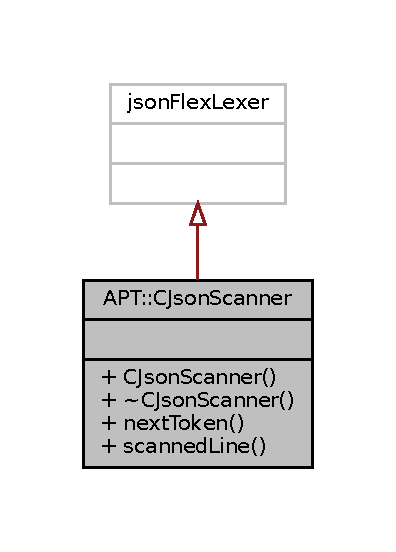
\includegraphics[width=190pt]{classAPT_1_1CJsonScanner__inherit__graph}
\end{center}
\end{figure}


Collaboration diagram for A\+PT\+:\+:C\+Json\+Scanner\+:
\nopagebreak
\begin{figure}[H]
\begin{center}
\leavevmode
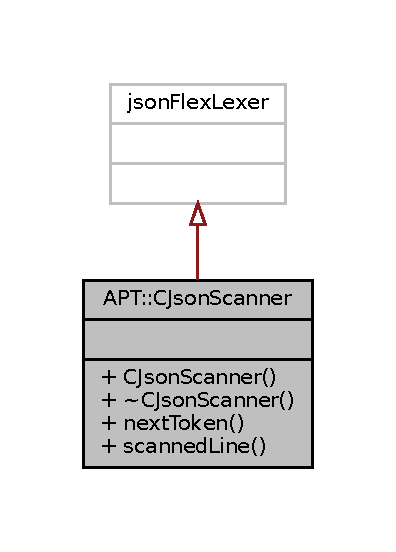
\includegraphics[width=190pt]{classAPT_1_1CJsonScanner__coll__graph}
\end{center}
\end{figure}
\subsection*{Public Member Functions}
\begin{DoxyCompactItemize}
\item 
\hyperlink{classAPT_1_1CJsonScanner_a66b75b3be7d072f0b51b17399a372b4b}{C\+Json\+Scanner} (std\+::istream \&input)
\item 
\hyperlink{classAPT_1_1CJsonScanner_a3ddc04d78015157e8e52df2cd6317330}{$\sim$\+C\+Json\+Scanner} ()
\item 
\hyperlink{classAPT_1_1CJsonToken}{C\+Json\+Token} $\ast$ \hyperlink{classAPT_1_1CJsonScanner_afe3b93ec865d0a77c31df6966e6fc4e1}{next\+Token} ()
\item 
int \hyperlink{classAPT_1_1CJsonScanner_adf983e640d42df3a5796b9f2aa2df5c0}{scanned\+Line} ()
\end{DoxyCompactItemize}


\subsection{Constructor \& Destructor Documentation}
\mbox{\Hypertarget{classAPT_1_1CJsonScanner_a66b75b3be7d072f0b51b17399a372b4b}\label{classAPT_1_1CJsonScanner_a66b75b3be7d072f0b51b17399a372b4b}} 
\index{A\+P\+T\+::\+C\+Json\+Scanner@{A\+P\+T\+::\+C\+Json\+Scanner}!C\+Json\+Scanner@{C\+Json\+Scanner}}
\index{C\+Json\+Scanner@{C\+Json\+Scanner}!A\+P\+T\+::\+C\+Json\+Scanner@{A\+P\+T\+::\+C\+Json\+Scanner}}
\subsubsection{\texorpdfstring{C\+Json\+Scanner()}{CJsonScanner()}}
{\footnotesize\ttfamily A\+P\+T\+::\+C\+Json\+Scanner\+::\+C\+Json\+Scanner (\begin{DoxyParamCaption}\item[{std\+::istream \&}]{input }\end{DoxyParamCaption})}

Create a new scanner that reads the given input stream. \mbox{\Hypertarget{classAPT_1_1CJsonScanner_a3ddc04d78015157e8e52df2cd6317330}\label{classAPT_1_1CJsonScanner_a3ddc04d78015157e8e52df2cd6317330}} 
\index{A\+P\+T\+::\+C\+Json\+Scanner@{A\+P\+T\+::\+C\+Json\+Scanner}!````~C\+Json\+Scanner@{$\sim$\+C\+Json\+Scanner}}
\index{````~C\+Json\+Scanner@{$\sim$\+C\+Json\+Scanner}!A\+P\+T\+::\+C\+Json\+Scanner@{A\+P\+T\+::\+C\+Json\+Scanner}}
\subsubsection{\texorpdfstring{$\sim$\+C\+Json\+Scanner()}{~CJsonScanner()}}
{\footnotesize\ttfamily A\+P\+T\+::\+C\+Json\+Scanner\+::$\sim$\+C\+Json\+Scanner (\begin{DoxyParamCaption}{ }\end{DoxyParamCaption})}

Frees all allocated resources. 

\subsection{Member Function Documentation}
\mbox{\Hypertarget{classAPT_1_1CJsonScanner_afe3b93ec865d0a77c31df6966e6fc4e1}\label{classAPT_1_1CJsonScanner_afe3b93ec865d0a77c31df6966e6fc4e1}} 
\index{A\+P\+T\+::\+C\+Json\+Scanner@{A\+P\+T\+::\+C\+Json\+Scanner}!next\+Token@{next\+Token}}
\index{next\+Token@{next\+Token}!A\+P\+T\+::\+C\+Json\+Scanner@{A\+P\+T\+::\+C\+Json\+Scanner}}
\subsubsection{\texorpdfstring{next\+Token()}{nextToken()}}
{\footnotesize\ttfamily \hyperlink{classAPT_1_1CJsonToken}{C\+Json\+Token} $\ast$ A\+P\+T\+::\+C\+Json\+Scanner\+::next\+Token (\begin{DoxyParamCaption}{ }\end{DoxyParamCaption})}

Returns the next token from the input. The pointer returned points to an object managed by this class. It is only valid until the next invocation of the method.

If the input is exhausted, the method returns 0. \mbox{\Hypertarget{classAPT_1_1CJsonScanner_adf983e640d42df3a5796b9f2aa2df5c0}\label{classAPT_1_1CJsonScanner_adf983e640d42df3a5796b9f2aa2df5c0}} 
\index{A\+P\+T\+::\+C\+Json\+Scanner@{A\+P\+T\+::\+C\+Json\+Scanner}!scanned\+Line@{scanned\+Line}}
\index{scanned\+Line@{scanned\+Line}!A\+P\+T\+::\+C\+Json\+Scanner@{A\+P\+T\+::\+C\+Json\+Scanner}}
\subsubsection{\texorpdfstring{scanned\+Line()}{scannedLine()}}
{\footnotesize\ttfamily int A\+P\+T\+::\+C\+Json\+Scanner\+::scanned\+Line (\begin{DoxyParamCaption}{ }\end{DoxyParamCaption})}

Return the line number of the input where last token (returned by \hyperlink{classAPT_1_1CJsonScanner_afe3b93ec865d0a77c31df6966e6fc4e1}{next\+Token()}) was found. 

The documentation for this class was generated from the following files\+:\begin{DoxyCompactItemize}
\item 
\hyperlink{CJsonScanner_8h}{C\+Json\+Scanner.\+h}\item 
\hyperlink{CJsonScanner_8cpp}{C\+Json\+Scanner.\+cpp}\end{DoxyCompactItemize}

\hypertarget{classAPT_1_1CJsonToken}{}\section{A\+PT\+:\+:C\+Json\+Token Class Reference}
\label{classAPT_1_1CJsonToken}\index{A\+P\+T\+::\+C\+Json\+Token@{A\+P\+T\+::\+C\+Json\+Token}}


{\ttfamily \#include $<$C\+Json\+Token.\+h$>$}



Inheritance diagram for A\+PT\+:\+:C\+Json\+Token\+:
\nopagebreak
\begin{figure}[H]
\begin{center}
\leavevmode
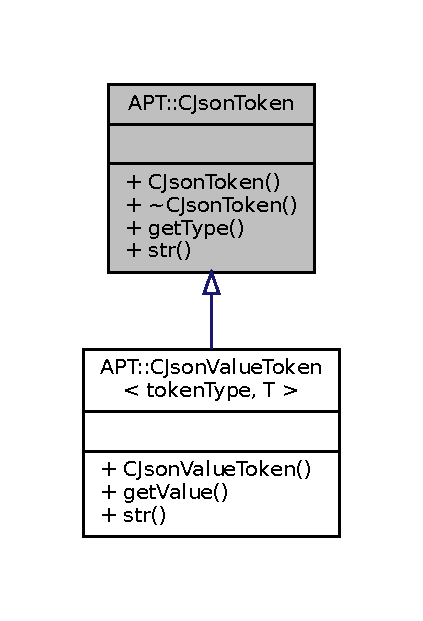
\includegraphics[width=203pt]{classAPT_1_1CJsonToken__inherit__graph}
\end{center}
\end{figure}


Collaboration diagram for A\+PT\+:\+:C\+Json\+Token\+:
\nopagebreak
\begin{figure}[H]
\begin{center}
\leavevmode
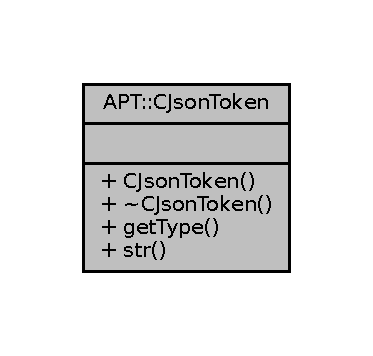
\includegraphics[width=179pt]{classAPT_1_1CJsonToken__coll__graph}
\end{center}
\end{figure}
\subsection*{Public Types}
\begin{DoxyCompactItemize}
\item 
enum \hyperlink{classAPT_1_1CJsonToken_aab8edca6cac7d6c2cd4cb37ea0ab0dce}{Token\+Type} \{ \newline
\hyperlink{classAPT_1_1CJsonToken_aab8edca6cac7d6c2cd4cb37ea0ab0dcea1f2a8e9d11469210748565d9da76292d}{B\+E\+G\+I\+N\+\_\+\+O\+B\+J\+E\+CT}, 
\hyperlink{classAPT_1_1CJsonToken_aab8edca6cac7d6c2cd4cb37ea0ab0dceac9243025ab521a5a32566508563d51f7}{E\+N\+D\+\_\+\+O\+B\+J\+E\+CT}, 
\hyperlink{classAPT_1_1CJsonToken_aab8edca6cac7d6c2cd4cb37ea0ab0dcea6633a9e242838039ada90488b43fd51e}{B\+E\+G\+I\+N\+\_\+\+A\+R\+R\+AY}, 
\hyperlink{classAPT_1_1CJsonToken_aab8edca6cac7d6c2cd4cb37ea0ab0dceaa946046468b4c5948681b0bf26df93ba}{E\+N\+D\+\_\+\+A\+R\+R\+AY}, 
\newline
\hyperlink{classAPT_1_1CJsonToken_aab8edca6cac7d6c2cd4cb37ea0ab0dceae528ae32d2650162babc271e55d01a6f}{N\+A\+M\+E\+\_\+\+S\+E\+P\+A\+R\+A\+T\+OR}, 
\hyperlink{classAPT_1_1CJsonToken_aab8edca6cac7d6c2cd4cb37ea0ab0dcea92e9f88204ae860c01f442a027ef1b6f}{V\+A\+L\+U\+E\+\_\+\+S\+E\+P\+A\+R\+A\+T\+OR}, 
\hyperlink{classAPT_1_1CJsonToken_aab8edca6cac7d6c2cd4cb37ea0ab0dceab38d27c8c3b0aa088ce14682895b19d0}{S\+T\+R\+I\+NG}, 
\hyperlink{classAPT_1_1CJsonToken_aab8edca6cac7d6c2cd4cb37ea0ab0dcea3113bd34020b4bff6e98c04ebc59cf1f}{N\+U\+M\+B\+ER}, 
\newline
\hyperlink{classAPT_1_1CJsonToken_aab8edca6cac7d6c2cd4cb37ea0ab0dceabee35e13f6e1392c313da66ffe95564e}{B\+O\+OL}, 
\hyperlink{classAPT_1_1CJsonToken_aab8edca6cac7d6c2cd4cb37ea0ab0dcea780fac87793f6b528a629e45b89cb895}{J\+S\+O\+N\+\_\+\+N\+U\+LL}
 \}
\end{DoxyCompactItemize}
\subsection*{Public Member Functions}
\begin{DoxyCompactItemize}
\item 
\hyperlink{classAPT_1_1CJsonToken_a02880c73b5e48fa4912297fe304c1265}{C\+Json\+Token} (\hyperlink{classAPT_1_1CJsonToken_aab8edca6cac7d6c2cd4cb37ea0ab0dce}{Token\+Type} type)
\item 
virtual \hyperlink{classAPT_1_1CJsonToken_a89e1a2e9eab654d5be172e7fd9555be1}{$\sim$\+C\+Json\+Token} ()
\item 
\hyperlink{classAPT_1_1CJsonToken_aab8edca6cac7d6c2cd4cb37ea0ab0dce}{Token\+Type} \hyperlink{classAPT_1_1CJsonToken_ab06f02d48757bfc68fb041fcafd680f6}{get\+Type} ()
\item 
virtual std\+::string \hyperlink{classAPT_1_1CJsonToken_a743343b64c20d0aa726d271c2b0e9be8}{str} ()
\end{DoxyCompactItemize}


\subsection{Detailed Description}
This is the base class for all tokens. It provides the token type. 

\subsection{Member Enumeration Documentation}
\mbox{\Hypertarget{classAPT_1_1CJsonToken_aab8edca6cac7d6c2cd4cb37ea0ab0dce}\label{classAPT_1_1CJsonToken_aab8edca6cac7d6c2cd4cb37ea0ab0dce}} 
\index{A\+P\+T\+::\+C\+Json\+Token@{A\+P\+T\+::\+C\+Json\+Token}!Token\+Type@{Token\+Type}}
\index{Token\+Type@{Token\+Type}!A\+P\+T\+::\+C\+Json\+Token@{A\+P\+T\+::\+C\+Json\+Token}}
\subsubsection{\texorpdfstring{Token\+Type}{TokenType}}
{\footnotesize\ttfamily enum \hyperlink{classAPT_1_1CJsonToken_aab8edca6cac7d6c2cd4cb37ea0ab0dce}{A\+P\+T\+::\+C\+Json\+Token\+::\+Token\+Type}}

The different token types. See R\+F\+C7159 (\href{https://tools.ietf.org/html/rfc7159}{\tt https\+://tools.\+ietf.\+org/html/rfc7159}). \begin{DoxyEnumFields}{Enumerator}
\raisebox{\heightof{T}}[0pt][0pt]{\index{B\+E\+G\+I\+N\+\_\+\+O\+B\+J\+E\+CT@{B\+E\+G\+I\+N\+\_\+\+O\+B\+J\+E\+CT}!A\+P\+T\+::\+C\+Json\+Token@{A\+P\+T\+::\+C\+Json\+Token}}\index{A\+P\+T\+::\+C\+Json\+Token@{A\+P\+T\+::\+C\+Json\+Token}!B\+E\+G\+I\+N\+\_\+\+O\+B\+J\+E\+CT@{B\+E\+G\+I\+N\+\_\+\+O\+B\+J\+E\+CT}}}\mbox{\Hypertarget{classAPT_1_1CJsonToken_aab8edca6cac7d6c2cd4cb37ea0ab0dcea1f2a8e9d11469210748565d9da76292d}\label{classAPT_1_1CJsonToken_aab8edca6cac7d6c2cd4cb37ea0ab0dcea1f2a8e9d11469210748565d9da76292d}} 
B\+E\+G\+I\+N\+\_\+\+O\+B\+J\+E\+CT&\\
\hline

\raisebox{\heightof{T}}[0pt][0pt]{\index{E\+N\+D\+\_\+\+O\+B\+J\+E\+CT@{E\+N\+D\+\_\+\+O\+B\+J\+E\+CT}!A\+P\+T\+::\+C\+Json\+Token@{A\+P\+T\+::\+C\+Json\+Token}}\index{A\+P\+T\+::\+C\+Json\+Token@{A\+P\+T\+::\+C\+Json\+Token}!E\+N\+D\+\_\+\+O\+B\+J\+E\+CT@{E\+N\+D\+\_\+\+O\+B\+J\+E\+CT}}}\mbox{\Hypertarget{classAPT_1_1CJsonToken_aab8edca6cac7d6c2cd4cb37ea0ab0dceac9243025ab521a5a32566508563d51f7}\label{classAPT_1_1CJsonToken_aab8edca6cac7d6c2cd4cb37ea0ab0dceac9243025ab521a5a32566508563d51f7}} 
E\+N\+D\+\_\+\+O\+B\+J\+E\+CT&\\
\hline

\raisebox{\heightof{T}}[0pt][0pt]{\index{B\+E\+G\+I\+N\+\_\+\+A\+R\+R\+AY@{B\+E\+G\+I\+N\+\_\+\+A\+R\+R\+AY}!A\+P\+T\+::\+C\+Json\+Token@{A\+P\+T\+::\+C\+Json\+Token}}\index{A\+P\+T\+::\+C\+Json\+Token@{A\+P\+T\+::\+C\+Json\+Token}!B\+E\+G\+I\+N\+\_\+\+A\+R\+R\+AY@{B\+E\+G\+I\+N\+\_\+\+A\+R\+R\+AY}}}\mbox{\Hypertarget{classAPT_1_1CJsonToken_aab8edca6cac7d6c2cd4cb37ea0ab0dcea6633a9e242838039ada90488b43fd51e}\label{classAPT_1_1CJsonToken_aab8edca6cac7d6c2cd4cb37ea0ab0dcea6633a9e242838039ada90488b43fd51e}} 
B\+E\+G\+I\+N\+\_\+\+A\+R\+R\+AY&\\
\hline

\raisebox{\heightof{T}}[0pt][0pt]{\index{E\+N\+D\+\_\+\+A\+R\+R\+AY@{E\+N\+D\+\_\+\+A\+R\+R\+AY}!A\+P\+T\+::\+C\+Json\+Token@{A\+P\+T\+::\+C\+Json\+Token}}\index{A\+P\+T\+::\+C\+Json\+Token@{A\+P\+T\+::\+C\+Json\+Token}!E\+N\+D\+\_\+\+A\+R\+R\+AY@{E\+N\+D\+\_\+\+A\+R\+R\+AY}}}\mbox{\Hypertarget{classAPT_1_1CJsonToken_aab8edca6cac7d6c2cd4cb37ea0ab0dceaa946046468b4c5948681b0bf26df93ba}\label{classAPT_1_1CJsonToken_aab8edca6cac7d6c2cd4cb37ea0ab0dceaa946046468b4c5948681b0bf26df93ba}} 
E\+N\+D\+\_\+\+A\+R\+R\+AY&\\
\hline

\raisebox{\heightof{T}}[0pt][0pt]{\index{N\+A\+M\+E\+\_\+\+S\+E\+P\+A\+R\+A\+T\+OR@{N\+A\+M\+E\+\_\+\+S\+E\+P\+A\+R\+A\+T\+OR}!A\+P\+T\+::\+C\+Json\+Token@{A\+P\+T\+::\+C\+Json\+Token}}\index{A\+P\+T\+::\+C\+Json\+Token@{A\+P\+T\+::\+C\+Json\+Token}!N\+A\+M\+E\+\_\+\+S\+E\+P\+A\+R\+A\+T\+OR@{N\+A\+M\+E\+\_\+\+S\+E\+P\+A\+R\+A\+T\+OR}}}\mbox{\Hypertarget{classAPT_1_1CJsonToken_aab8edca6cac7d6c2cd4cb37ea0ab0dceae528ae32d2650162babc271e55d01a6f}\label{classAPT_1_1CJsonToken_aab8edca6cac7d6c2cd4cb37ea0ab0dceae528ae32d2650162babc271e55d01a6f}} 
N\+A\+M\+E\+\_\+\+S\+E\+P\+A\+R\+A\+T\+OR&\\
\hline

\raisebox{\heightof{T}}[0pt][0pt]{\index{V\+A\+L\+U\+E\+\_\+\+S\+E\+P\+A\+R\+A\+T\+OR@{V\+A\+L\+U\+E\+\_\+\+S\+E\+P\+A\+R\+A\+T\+OR}!A\+P\+T\+::\+C\+Json\+Token@{A\+P\+T\+::\+C\+Json\+Token}}\index{A\+P\+T\+::\+C\+Json\+Token@{A\+P\+T\+::\+C\+Json\+Token}!V\+A\+L\+U\+E\+\_\+\+S\+E\+P\+A\+R\+A\+T\+OR@{V\+A\+L\+U\+E\+\_\+\+S\+E\+P\+A\+R\+A\+T\+OR}}}\mbox{\Hypertarget{classAPT_1_1CJsonToken_aab8edca6cac7d6c2cd4cb37ea0ab0dcea92e9f88204ae860c01f442a027ef1b6f}\label{classAPT_1_1CJsonToken_aab8edca6cac7d6c2cd4cb37ea0ab0dcea92e9f88204ae860c01f442a027ef1b6f}} 
V\+A\+L\+U\+E\+\_\+\+S\+E\+P\+A\+R\+A\+T\+OR&\\
\hline

\raisebox{\heightof{T}}[0pt][0pt]{\index{S\+T\+R\+I\+NG@{S\+T\+R\+I\+NG}!A\+P\+T\+::\+C\+Json\+Token@{A\+P\+T\+::\+C\+Json\+Token}}\index{A\+P\+T\+::\+C\+Json\+Token@{A\+P\+T\+::\+C\+Json\+Token}!S\+T\+R\+I\+NG@{S\+T\+R\+I\+NG}}}\mbox{\Hypertarget{classAPT_1_1CJsonToken_aab8edca6cac7d6c2cd4cb37ea0ab0dceab38d27c8c3b0aa088ce14682895b19d0}\label{classAPT_1_1CJsonToken_aab8edca6cac7d6c2cd4cb37ea0ab0dceab38d27c8c3b0aa088ce14682895b19d0}} 
S\+T\+R\+I\+NG&\\
\hline

\raisebox{\heightof{T}}[0pt][0pt]{\index{N\+U\+M\+B\+ER@{N\+U\+M\+B\+ER}!A\+P\+T\+::\+C\+Json\+Token@{A\+P\+T\+::\+C\+Json\+Token}}\index{A\+P\+T\+::\+C\+Json\+Token@{A\+P\+T\+::\+C\+Json\+Token}!N\+U\+M\+B\+ER@{N\+U\+M\+B\+ER}}}\mbox{\Hypertarget{classAPT_1_1CJsonToken_aab8edca6cac7d6c2cd4cb37ea0ab0dcea3113bd34020b4bff6e98c04ebc59cf1f}\label{classAPT_1_1CJsonToken_aab8edca6cac7d6c2cd4cb37ea0ab0dcea3113bd34020b4bff6e98c04ebc59cf1f}} 
N\+U\+M\+B\+ER&\\
\hline

\raisebox{\heightof{T}}[0pt][0pt]{\index{B\+O\+OL@{B\+O\+OL}!A\+P\+T\+::\+C\+Json\+Token@{A\+P\+T\+::\+C\+Json\+Token}}\index{A\+P\+T\+::\+C\+Json\+Token@{A\+P\+T\+::\+C\+Json\+Token}!B\+O\+OL@{B\+O\+OL}}}\mbox{\Hypertarget{classAPT_1_1CJsonToken_aab8edca6cac7d6c2cd4cb37ea0ab0dceabee35e13f6e1392c313da66ffe95564e}\label{classAPT_1_1CJsonToken_aab8edca6cac7d6c2cd4cb37ea0ab0dceabee35e13f6e1392c313da66ffe95564e}} 
B\+O\+OL&\\
\hline

\raisebox{\heightof{T}}[0pt][0pt]{\index{J\+S\+O\+N\+\_\+\+N\+U\+LL@{J\+S\+O\+N\+\_\+\+N\+U\+LL}!A\+P\+T\+::\+C\+Json\+Token@{A\+P\+T\+::\+C\+Json\+Token}}\index{A\+P\+T\+::\+C\+Json\+Token@{A\+P\+T\+::\+C\+Json\+Token}!J\+S\+O\+N\+\_\+\+N\+U\+LL@{J\+S\+O\+N\+\_\+\+N\+U\+LL}}}\mbox{\Hypertarget{classAPT_1_1CJsonToken_aab8edca6cac7d6c2cd4cb37ea0ab0dcea780fac87793f6b528a629e45b89cb895}\label{classAPT_1_1CJsonToken_aab8edca6cac7d6c2cd4cb37ea0ab0dcea780fac87793f6b528a629e45b89cb895}} 
J\+S\+O\+N\+\_\+\+N\+U\+LL&\\
\hline

\end{DoxyEnumFields}


\subsection{Constructor \& Destructor Documentation}
\mbox{\Hypertarget{classAPT_1_1CJsonToken_a02880c73b5e48fa4912297fe304c1265}\label{classAPT_1_1CJsonToken_a02880c73b5e48fa4912297fe304c1265}} 
\index{A\+P\+T\+::\+C\+Json\+Token@{A\+P\+T\+::\+C\+Json\+Token}!C\+Json\+Token@{C\+Json\+Token}}
\index{C\+Json\+Token@{C\+Json\+Token}!A\+P\+T\+::\+C\+Json\+Token@{A\+P\+T\+::\+C\+Json\+Token}}
\subsubsection{\texorpdfstring{C\+Json\+Token()}{CJsonToken()}}
{\footnotesize\ttfamily A\+P\+T\+::\+C\+Json\+Token\+::\+C\+Json\+Token (\begin{DoxyParamCaption}\item[{\hyperlink{classAPT_1_1CJsonToken_aab8edca6cac7d6c2cd4cb37ea0ab0dce}{Token\+Type}}]{type }\end{DoxyParamCaption})}

\mbox{\Hypertarget{classAPT_1_1CJsonToken_a89e1a2e9eab654d5be172e7fd9555be1}\label{classAPT_1_1CJsonToken_a89e1a2e9eab654d5be172e7fd9555be1}} 
\index{A\+P\+T\+::\+C\+Json\+Token@{A\+P\+T\+::\+C\+Json\+Token}!````~C\+Json\+Token@{$\sim$\+C\+Json\+Token}}
\index{````~C\+Json\+Token@{$\sim$\+C\+Json\+Token}!A\+P\+T\+::\+C\+Json\+Token@{A\+P\+T\+::\+C\+Json\+Token}}
\subsubsection{\texorpdfstring{$\sim$\+C\+Json\+Token()}{~CJsonToken()}}
{\footnotesize\ttfamily A\+P\+T\+::\+C\+Json\+Token\+::$\sim$\+C\+Json\+Token (\begin{DoxyParamCaption}{ }\end{DoxyParamCaption})\hspace{0.3cm}{\ttfamily [virtual]}}



\subsection{Member Function Documentation}
\mbox{\Hypertarget{classAPT_1_1CJsonToken_ab06f02d48757bfc68fb041fcafd680f6}\label{classAPT_1_1CJsonToken_ab06f02d48757bfc68fb041fcafd680f6}} 
\index{A\+P\+T\+::\+C\+Json\+Token@{A\+P\+T\+::\+C\+Json\+Token}!get\+Type@{get\+Type}}
\index{get\+Type@{get\+Type}!A\+P\+T\+::\+C\+Json\+Token@{A\+P\+T\+::\+C\+Json\+Token}}
\subsubsection{\texorpdfstring{get\+Type()}{getType()}}
{\footnotesize\ttfamily \hyperlink{classAPT_1_1CJsonToken_aab8edca6cac7d6c2cd4cb37ea0ab0dce}{C\+Json\+Token\+::\+Token\+Type} A\+P\+T\+::\+C\+Json\+Token\+::get\+Type (\begin{DoxyParamCaption}{ }\end{DoxyParamCaption})}

Return the type of the token. \mbox{\Hypertarget{classAPT_1_1CJsonToken_a743343b64c20d0aa726d271c2b0e9be8}\label{classAPT_1_1CJsonToken_a743343b64c20d0aa726d271c2b0e9be8}} 
\index{A\+P\+T\+::\+C\+Json\+Token@{A\+P\+T\+::\+C\+Json\+Token}!str@{str}}
\index{str@{str}!A\+P\+T\+::\+C\+Json\+Token@{A\+P\+T\+::\+C\+Json\+Token}}
\subsubsection{\texorpdfstring{str()}{str()}}
{\footnotesize\ttfamily string A\+P\+T\+::\+C\+Json\+Token\+::str (\begin{DoxyParamCaption}{ }\end{DoxyParamCaption})\hspace{0.3cm}{\ttfamily [virtual]}}

Allow convertion to string. 

Reimplemented in \hyperlink{classAPT_1_1CJsonValueToken_ab7d49b06f5242abfb7e67fa10278690b}{A\+P\+T\+::\+C\+Json\+Value\+Token$<$ token\+Type, T $>$}.



The documentation for this class was generated from the following files\+:\begin{DoxyCompactItemize}
\item 
\hyperlink{CJsonToken_8h}{C\+Json\+Token.\+h}\item 
\hyperlink{CJsonToken_8cpp}{C\+Json\+Token.\+cpp}\end{DoxyCompactItemize}

\hypertarget{classAPT_1_1CJsonValueToken}{}\section{A\+PT\+:\+:C\+Json\+Value\+Token$<$ token\+Type, T $>$ Class Template Reference}
\label{classAPT_1_1CJsonValueToken}\index{A\+P\+T\+::\+C\+Json\+Value\+Token$<$ token\+Type, T $>$@{A\+P\+T\+::\+C\+Json\+Value\+Token$<$ token\+Type, T $>$}}


{\ttfamily \#include $<$C\+Json\+Token.\+h$>$}



Inheritance diagram for A\+PT\+:\+:C\+Json\+Value\+Token$<$ token\+Type, T $>$\+:
\nopagebreak
\begin{figure}[H]
\begin{center}
\leavevmode
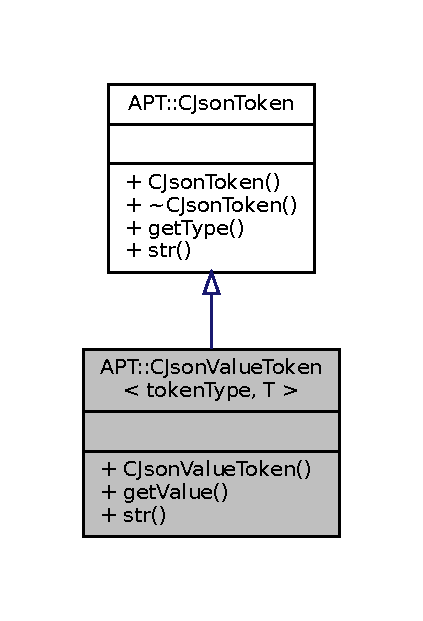
\includegraphics[width=203pt]{classAPT_1_1CJsonValueToken__inherit__graph}
\end{center}
\end{figure}


Collaboration diagram for A\+PT\+:\+:C\+Json\+Value\+Token$<$ token\+Type, T $>$\+:
\nopagebreak
\begin{figure}[H]
\begin{center}
\leavevmode
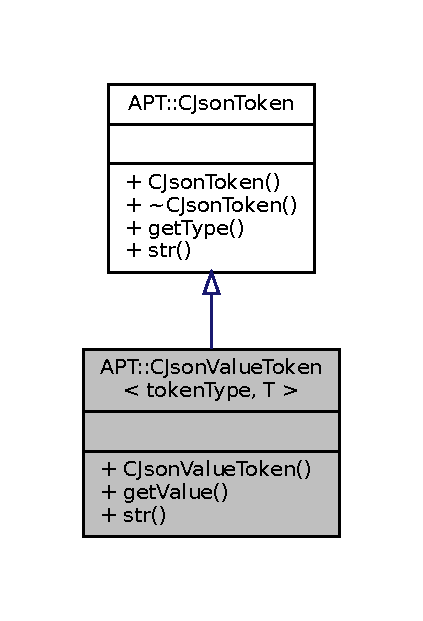
\includegraphics[width=203pt]{classAPT_1_1CJsonValueToken__coll__graph}
\end{center}
\end{figure}
\subsection*{Public Member Functions}
\begin{DoxyCompactItemize}
\item 
\hyperlink{classAPT_1_1CJsonValueToken_a8c037f13ded3735b427a5d2738208df8}{C\+Json\+Value\+Token} (T value)
\item 
T \hyperlink{classAPT_1_1CJsonValueToken_a352489d038676e08aba9f8b06f932c88}{get\+Value} () const
\item 
std\+::string \hyperlink{classAPT_1_1CJsonValueToken_ab7d49b06f5242abfb7e67fa10278690b}{str} ()
\end{DoxyCompactItemize}
\subsection*{Additional Inherited Members}


\subsection{Detailed Description}
\subsubsection*{template$<$C\+Json\+Token\+::\+Token\+Type token\+Type, class T$>$\newline
class A\+P\+T\+::\+C\+Json\+Value\+Token$<$ token\+Type, T $>$}

This template is used to define special tokens that have an associated value of the given type. This is not intended to be used by programmers. Use the derived types C\+Json\+String\+Token, C\+Json\+Number\+Token and C\+Json\+Bool\+Token instead. 

\subsection{Constructor \& Destructor Documentation}
\mbox{\Hypertarget{classAPT_1_1CJsonValueToken_a8c037f13ded3735b427a5d2738208df8}\label{classAPT_1_1CJsonValueToken_a8c037f13ded3735b427a5d2738208df8}} 
\index{A\+P\+T\+::\+C\+Json\+Value\+Token@{A\+P\+T\+::\+C\+Json\+Value\+Token}!C\+Json\+Value\+Token@{C\+Json\+Value\+Token}}
\index{C\+Json\+Value\+Token@{C\+Json\+Value\+Token}!A\+P\+T\+::\+C\+Json\+Value\+Token@{A\+P\+T\+::\+C\+Json\+Value\+Token}}
\subsubsection{\texorpdfstring{C\+Json\+Value\+Token()}{CJsonValueToken()}}
{\footnotesize\ttfamily template$<$C\+Json\+Token\+::\+Token\+Type token\+Type, class T $>$ \\
\hyperlink{classAPT_1_1CJsonValueToken}{A\+P\+T\+::\+C\+Json\+Value\+Token}$<$ token\+Type, T $>$\+::\hyperlink{classAPT_1_1CJsonValueToken}{C\+Json\+Value\+Token} (\begin{DoxyParamCaption}\item[{T}]{value }\end{DoxyParamCaption})\hspace{0.3cm}{\ttfamily [inline]}}

Create a token with the given value. 

\subsection{Member Function Documentation}
\mbox{\Hypertarget{classAPT_1_1CJsonValueToken_a352489d038676e08aba9f8b06f932c88}\label{classAPT_1_1CJsonValueToken_a352489d038676e08aba9f8b06f932c88}} 
\index{A\+P\+T\+::\+C\+Json\+Value\+Token@{A\+P\+T\+::\+C\+Json\+Value\+Token}!get\+Value@{get\+Value}}
\index{get\+Value@{get\+Value}!A\+P\+T\+::\+C\+Json\+Value\+Token@{A\+P\+T\+::\+C\+Json\+Value\+Token}}
\subsubsection{\texorpdfstring{get\+Value()}{getValue()}}
{\footnotesize\ttfamily template$<$C\+Json\+Token\+::\+Token\+Type token\+Type, class T $>$ \\
T \hyperlink{classAPT_1_1CJsonValueToken}{A\+P\+T\+::\+C\+Json\+Value\+Token}$<$ token\+Type, T $>$\+::get\+Value (\begin{DoxyParamCaption}{ }\end{DoxyParamCaption}) const\hspace{0.3cm}{\ttfamily [inline]}}

Return the value associated with the token. \mbox{\Hypertarget{classAPT_1_1CJsonValueToken_ab7d49b06f5242abfb7e67fa10278690b}\label{classAPT_1_1CJsonValueToken_ab7d49b06f5242abfb7e67fa10278690b}} 
\index{A\+P\+T\+::\+C\+Json\+Value\+Token@{A\+P\+T\+::\+C\+Json\+Value\+Token}!str@{str}}
\index{str@{str}!A\+P\+T\+::\+C\+Json\+Value\+Token@{A\+P\+T\+::\+C\+Json\+Value\+Token}}
\subsubsection{\texorpdfstring{str()}{str()}}
{\footnotesize\ttfamily template$<$C\+Json\+Token\+::\+Token\+Type token\+Type, class T $>$ \\
std\+::string \hyperlink{classAPT_1_1CJsonValueToken}{A\+P\+T\+::\+C\+Json\+Value\+Token}$<$ token\+Type, T $>$\+::str (\begin{DoxyParamCaption}{ }\end{DoxyParamCaption})\hspace{0.3cm}{\ttfamily [inline]}, {\ttfamily [virtual]}}

Allow convertion to string. 

Reimplemented from \hyperlink{classAPT_1_1CJsonToken_a743343b64c20d0aa726d271c2b0e9be8}{A\+P\+T\+::\+C\+Json\+Token}.



The documentation for this class was generated from the following file\+:\begin{DoxyCompactItemize}
\item 
\hyperlink{CJsonToken_8h}{C\+Json\+Token.\+h}\end{DoxyCompactItemize}

\hypertarget{classCNavigationSystem}{}\section{C\+Navigation\+System Class Reference}
\label{classCNavigationSystem}\index{C\+Navigation\+System@{C\+Navigation\+System}}


{\ttfamily \#include $<$C\+Navigation\+System.\+h$>$}



Collaboration diagram for C\+Navigation\+System\+:
\nopagebreak
\begin{figure}[H]
\begin{center}
\leavevmode
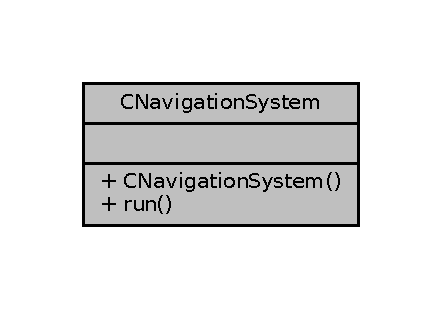
\includegraphics[width=212pt]{classCNavigationSystem__coll__graph}
\end{center}
\end{figure}
\subsection*{Public Member Functions}
\begin{DoxyCompactItemize}
\item 
\hyperlink{classCNavigationSystem_aa5e3856fa5efdbe6f2b25d974eb96c8f}{C\+Navigation\+System} ()
\item 
void \hyperlink{classCNavigationSystem_a51ad541b47891dc9a07abb61b68a8ad8}{run} ()
\end{DoxyCompactItemize}


\subsection{Constructor \& Destructor Documentation}
\mbox{\Hypertarget{classCNavigationSystem_aa5e3856fa5efdbe6f2b25d974eb96c8f}\label{classCNavigationSystem_aa5e3856fa5efdbe6f2b25d974eb96c8f}} 
\index{C\+Navigation\+System@{C\+Navigation\+System}!C\+Navigation\+System@{C\+Navigation\+System}}
\index{C\+Navigation\+System@{C\+Navigation\+System}!C\+Navigation\+System@{C\+Navigation\+System}}
\subsubsection{\texorpdfstring{C\+Navigation\+System()}{CNavigationSystem()}}
{\footnotesize\ttfamily C\+Navigation\+System\+::\+C\+Navigation\+System (\begin{DoxyParamCaption}{ }\end{DoxyParamCaption})}

Test\+Case to check if non existing P\+OI is added to the route  void Test\+Case to check if non existing Waypoint is added to the route  void Test\+Case to check when P\+OI database is not available  void Test\+Case to check when Waypoint database is not available  void Constructor

Constructor 

\subsection{Member Function Documentation}
\mbox{\Hypertarget{classCNavigationSystem_a51ad541b47891dc9a07abb61b68a8ad8}\label{classCNavigationSystem_a51ad541b47891dc9a07abb61b68a8ad8}} 
\index{C\+Navigation\+System@{C\+Navigation\+System}!run@{run}}
\index{run@{run}!C\+Navigation\+System@{C\+Navigation\+System}}
\subsubsection{\texorpdfstring{run()}{run()}}
{\footnotesize\ttfamily void C\+Navigation\+System\+::run (\begin{DoxyParamCaption}{ }\end{DoxyParamCaption})}

Navigation System functionaliy\textquotesingle{}s entry function  void 

The documentation for this class was generated from the following files\+:\begin{DoxyCompactItemize}
\item 
\hyperlink{CNavigationSystem_8h}{C\+Navigation\+System.\+h}\item 
\hyperlink{CNavigationSystem_8cpp}{C\+Navigation\+System.\+cpp}\end{DoxyCompactItemize}

\hypertarget{classCParser}{}\section{C\+Parser Class Reference}
\label{classCParser}\index{C\+Parser@{C\+Parser}}


{\ttfamily \#include $<$C\+Parser.\+h$>$}



Inheritance diagram for C\+Parser\+:
\nopagebreak
\begin{figure}[H]
\begin{center}
\leavevmode
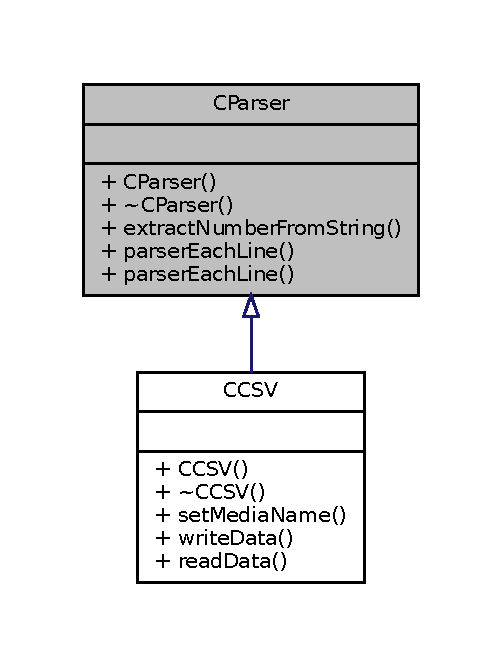
\includegraphics[width=241pt]{classCParser__inherit__graph}
\end{center}
\end{figure}


Collaboration diagram for C\+Parser\+:
\nopagebreak
\begin{figure}[H]
\begin{center}
\leavevmode
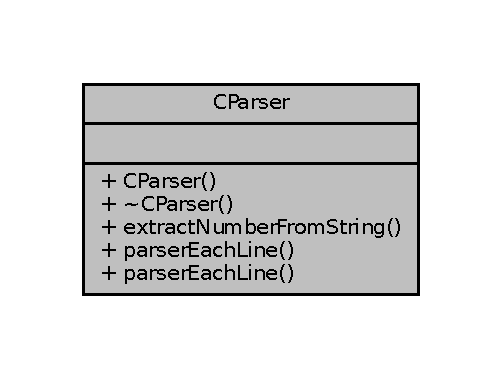
\includegraphics[width=241pt]{classCParser__coll__graph}
\end{center}
\end{figure}
\subsection*{Public Member Functions}
\begin{DoxyCompactItemize}
\item 
\hyperlink{classCParser_aa6372ef4dbf7d11dc4c51f4f4abd1750}{C\+Parser} ()
\item 
virtual \hyperlink{classCParser_acabd3b10aa5593fe571fe55426a7916f}{$\sim$\+C\+Parser} ()
\item 
bool \hyperlink{classCParser_a4bd9b28a9d6512c10b2b5af3ff36495f}{extract\+Number\+From\+String} (const std\+::string \&str, double \&number)
\item 
bool \hyperlink{classCParser_a2bfd12df0bb7928de4a0ad50230a2e19}{parser\+Each\+Line} (const std\+::string \&read\+Line, std\+::string \&name, double \&latitude, double \&longitude, const unsigned int line\+Counter)
\item 
bool \hyperlink{classCParser_a5d04d85e9ccaf568a50b7cfe071b7bf3}{parser\+Each\+Line} (const std\+::string \&read\+Line, \hyperlink{classCPOI_a4b95e2e14055d2f9ca134e474dd4a19f}{C\+P\+O\+I\+::t\+\_\+poi} \&type, std\+::string \&name, std\+::string \&description, double \&latitude, double \&longitude, const unsigned int line\+Counter)
\end{DoxyCompactItemize}


\subsection{Constructor \& Destructor Documentation}
\mbox{\Hypertarget{classCParser_aa6372ef4dbf7d11dc4c51f4f4abd1750}\label{classCParser_aa6372ef4dbf7d11dc4c51f4f4abd1750}} 
\index{C\+Parser@{C\+Parser}!C\+Parser@{C\+Parser}}
\index{C\+Parser@{C\+Parser}!C\+Parser@{C\+Parser}}
\subsubsection{\texorpdfstring{C\+Parser()}{CParser()}}
{\footnotesize\ttfamily C\+Parser\+::\+C\+Parser (\begin{DoxyParamCaption}{ }\end{DoxyParamCaption})}

\mbox{\Hypertarget{classCParser_acabd3b10aa5593fe571fe55426a7916f}\label{classCParser_acabd3b10aa5593fe571fe55426a7916f}} 
\index{C\+Parser@{C\+Parser}!````~C\+Parser@{$\sim$\+C\+Parser}}
\index{````~C\+Parser@{$\sim$\+C\+Parser}!C\+Parser@{C\+Parser}}
\subsubsection{\texorpdfstring{$\sim$\+C\+Parser()}{~CParser()}}
{\footnotesize\ttfamily C\+Parser\+::$\sim$\+C\+Parser (\begin{DoxyParamCaption}{ }\end{DoxyParamCaption})\hspace{0.3cm}{\ttfamily [virtual]}}



\subsection{Member Function Documentation}
\mbox{\Hypertarget{classCParser_a4bd9b28a9d6512c10b2b5af3ff36495f}\label{classCParser_a4bd9b28a9d6512c10b2b5af3ff36495f}} 
\index{C\+Parser@{C\+Parser}!extract\+Number\+From\+String@{extract\+Number\+From\+String}}
\index{extract\+Number\+From\+String@{extract\+Number\+From\+String}!C\+Parser@{C\+Parser}}
\subsubsection{\texorpdfstring{extract\+Number\+From\+String()}{extractNumberFromString()}}
{\footnotesize\ttfamily bool C\+Parser\+::extract\+Number\+From\+String (\begin{DoxyParamCaption}\item[{const std\+::string \&}]{str,  }\item[{double \&}]{number }\end{DoxyParamCaption})}

Extract number from the string 
\begin{DoxyParams}{Parameters}
{\em const} & string \&str -\/ string (IN) \\
\hline
{\em double} & \&number -\/ Number to return (O\+UT)  bool -\/ Success -\/ true or Failure -\/ false \\
\hline
\end{DoxyParams}
\mbox{\Hypertarget{classCParser_a2bfd12df0bb7928de4a0ad50230a2e19}\label{classCParser_a2bfd12df0bb7928de4a0ad50230a2e19}} 
\index{C\+Parser@{C\+Parser}!parser\+Each\+Line@{parser\+Each\+Line}}
\index{parser\+Each\+Line@{parser\+Each\+Line}!C\+Parser@{C\+Parser}}
\subsubsection{\texorpdfstring{parser\+Each\+Line()}{parserEachLine()}\hspace{0.1cm}{\footnotesize\ttfamily [1/2]}}
{\footnotesize\ttfamily bool C\+Parser\+::parser\+Each\+Line (\begin{DoxyParamCaption}\item[{const std\+::string \&}]{read\+Line,  }\item[{std\+::string \&}]{name,  }\item[{double \&}]{latitude,  }\item[{double \&}]{longitude,  }\item[{const unsigned int}]{line\+Counter }\end{DoxyParamCaption})}

Parse a line to get waypoint information such as name, latitude and longitude in order 
\begin{DoxyParams}{Parameters}
{\em const} & string \&read\+Line -\/ Each Line (IN) \\
\hline
{\em const} & string \&name -\/ name of waypoint (O\+UT) \\
\hline
{\em const} & double \&latitude -\/ latitude of waypoint (O\+UT) \\
\hline
{\em const} & double \&longitude -\/ longitude of waypoint (O\+UT)  bool -\/ Success -\/ true or Failure -\/ false \\
\hline
\end{DoxyParams}
\mbox{\Hypertarget{classCParser_a5d04d85e9ccaf568a50b7cfe071b7bf3}\label{classCParser_a5d04d85e9ccaf568a50b7cfe071b7bf3}} 
\index{C\+Parser@{C\+Parser}!parser\+Each\+Line@{parser\+Each\+Line}}
\index{parser\+Each\+Line@{parser\+Each\+Line}!C\+Parser@{C\+Parser}}
\subsubsection{\texorpdfstring{parser\+Each\+Line()}{parserEachLine()}\hspace{0.1cm}{\footnotesize\ttfamily [2/2]}}
{\footnotesize\ttfamily bool C\+Parser\+::parser\+Each\+Line (\begin{DoxyParamCaption}\item[{const std\+::string \&}]{read\+Line,  }\item[{\hyperlink{classCPOI_a4b95e2e14055d2f9ca134e474dd4a19f}{C\+P\+O\+I\+::t\+\_\+poi} \&}]{type,  }\item[{std\+::string \&}]{name,  }\item[{std\+::string \&}]{description,  }\item[{double \&}]{latitude,  }\item[{double \&}]{longitude,  }\item[{const unsigned int}]{line\+Counter }\end{DoxyParamCaption})}

Parse a line to get P\+OI information such as type, name, description, latitude and longitude in order 
\begin{DoxyParams}{Parameters}
{\em const} & string \&read\+Line -\/ Each Line (IN) \\
\hline
{\em const} & t\+\_\+poi \&type -\/ name of P\+OI (O\+UT) \\
\hline
{\em const} & string \&name -\/ name of P\+OI (O\+UT) \\
\hline
{\em const} & string \&description -\/ description of P\+OI (O\+UT) \\
\hline
{\em const} & double \&latitude -\/ latitude of P\+OI (O\+UT) \\
\hline
{\em const} & double \&longitude -\/ longitude of P\+OI (O\+UT)  bool -\/ Success -\/ true or Failure -\/ false \\
\hline
\end{DoxyParams}


The documentation for this class was generated from the following files\+:\begin{DoxyCompactItemize}
\item 
\hyperlink{CParser_8h}{C\+Parser.\+h}\item 
\hyperlink{CParser_8cpp}{C\+Parser.\+cpp}\end{DoxyCompactItemize}

\hypertarget{classCPersistentStorage}{}\section{C\+Persistent\+Storage Class Reference}
\label{classCPersistentStorage}\index{C\+Persistent\+Storage@{C\+Persistent\+Storage}}


{\ttfamily \#include $<$C\+Persistent\+Storage.\+h$>$}



Inheritance diagram for C\+Persistent\+Storage\+:
\nopagebreak
\begin{figure}[H]
\begin{center}
\leavevmode
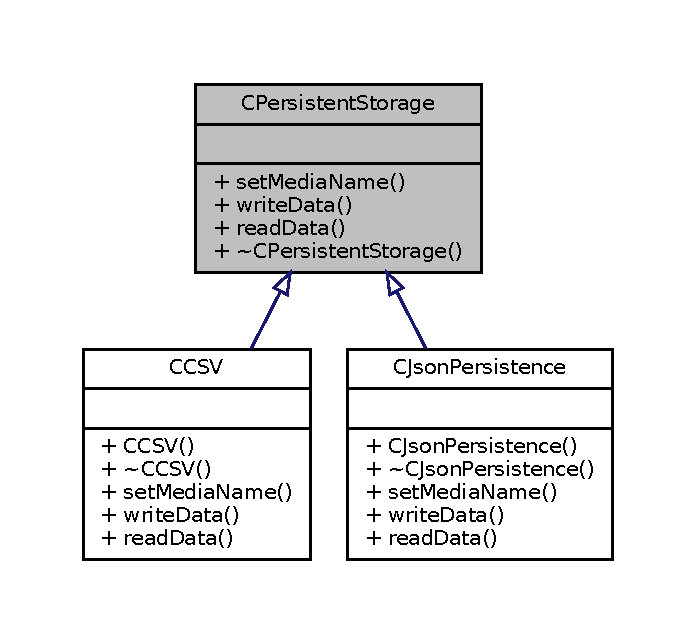
\includegraphics[width=334pt]{classCPersistentStorage__inherit__graph}
\end{center}
\end{figure}


Collaboration diagram for C\+Persistent\+Storage\+:
\nopagebreak
\begin{figure}[H]
\begin{center}
\leavevmode
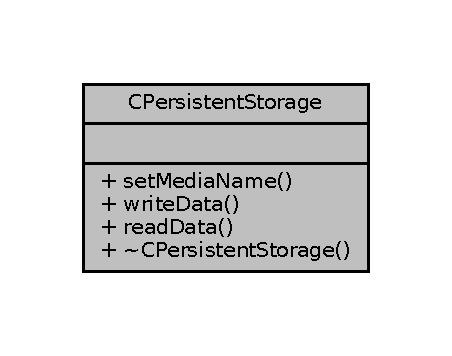
\includegraphics[width=217pt]{classCPersistentStorage__coll__graph}
\end{center}
\end{figure}
\subsection*{Public Types}
\begin{DoxyCompactItemize}
\item 
enum \hyperlink{classCPersistentStorage_a9b9929a4afa6e21da10f4a2e926a4584}{Merge\+Mode} \{ \hyperlink{classCPersistentStorage_a9b9929a4afa6e21da10f4a2e926a4584a61eb51fcd97853482d0436ea6b5fec2f}{M\+E\+R\+GE}, 
\hyperlink{classCPersistentStorage_a9b9929a4afa6e21da10f4a2e926a4584a5eb3db7839315215409a77d1c58230ac}{R\+E\+P\+L\+A\+CE}
 \}
\end{DoxyCompactItemize}
\subsection*{Public Member Functions}
\begin{DoxyCompactItemize}
\item 
virtual void \hyperlink{classCPersistentStorage_af626d001915346c04c2008c9ea8bb8d8}{set\+Media\+Name} (std\+::string name)=0
\item 
virtual bool \hyperlink{classCPersistentStorage_ab0c03dbf674c6218d574289ec54a75ed}{write\+Data} (const \hyperlink{classCWpDatabase}{C\+Wp\+Database} \&waypoint\+Db, const \hyperlink{classCPoiDatabase}{C\+Poi\+Database} \&poi\+Db)=0
\item 
virtual bool \hyperlink{classCPersistentStorage_a28edf547e10449a7f45de9885b68890b}{read\+Data} (\hyperlink{classCWpDatabase}{C\+Wp\+Database} \&waypoint\+Db, \hyperlink{classCPoiDatabase}{C\+Poi\+Database} \&poi\+Db, \hyperlink{classCPersistentStorage_a9b9929a4afa6e21da10f4a2e926a4584}{Merge\+Mode} mode)=0
\item 
virtual \hyperlink{classCPersistentStorage_a040e22bf1000853fbcd2ff45239386d9}{$\sim$\+C\+Persistent\+Storage} ()
\end{DoxyCompactItemize}


\subsection{Member Enumeration Documentation}
\mbox{\Hypertarget{classCPersistentStorage_a9b9929a4afa6e21da10f4a2e926a4584}\label{classCPersistentStorage_a9b9929a4afa6e21da10f4a2e926a4584}} 
\index{C\+Persistent\+Storage@{C\+Persistent\+Storage}!Merge\+Mode@{Merge\+Mode}}
\index{Merge\+Mode@{Merge\+Mode}!C\+Persistent\+Storage@{C\+Persistent\+Storage}}
\subsubsection{\texorpdfstring{Merge\+Mode}{MergeMode}}
{\footnotesize\ttfamily enum \hyperlink{classCPersistentStorage_a9b9929a4afa6e21da10f4a2e926a4584}{C\+Persistent\+Storage\+::\+Merge\+Mode}}

The mode to be used when reading the data bases (see read\+Data). \begin{DoxyEnumFields}{Enumerator}
\raisebox{\heightof{T}}[0pt][0pt]{\index{M\+E\+R\+GE@{M\+E\+R\+GE}!C\+Persistent\+Storage@{C\+Persistent\+Storage}}\index{C\+Persistent\+Storage@{C\+Persistent\+Storage}!M\+E\+R\+GE@{M\+E\+R\+GE}}}\mbox{\Hypertarget{classCPersistentStorage_a9b9929a4afa6e21da10f4a2e926a4584a61eb51fcd97853482d0436ea6b5fec2f}\label{classCPersistentStorage_a9b9929a4afa6e21da10f4a2e926a4584a61eb51fcd97853482d0436ea6b5fec2f}} 
M\+E\+R\+GE&\\
\hline

\raisebox{\heightof{T}}[0pt][0pt]{\index{R\+E\+P\+L\+A\+CE@{R\+E\+P\+L\+A\+CE}!C\+Persistent\+Storage@{C\+Persistent\+Storage}}\index{C\+Persistent\+Storage@{C\+Persistent\+Storage}!R\+E\+P\+L\+A\+CE@{R\+E\+P\+L\+A\+CE}}}\mbox{\Hypertarget{classCPersistentStorage_a9b9929a4afa6e21da10f4a2e926a4584a5eb3db7839315215409a77d1c58230ac}\label{classCPersistentStorage_a9b9929a4afa6e21da10f4a2e926a4584a5eb3db7839315215409a77d1c58230ac}} 
R\+E\+P\+L\+A\+CE&\\
\hline

\end{DoxyEnumFields}


\subsection{Constructor \& Destructor Documentation}
\mbox{\Hypertarget{classCPersistentStorage_a040e22bf1000853fbcd2ff45239386d9}\label{classCPersistentStorage_a040e22bf1000853fbcd2ff45239386d9}} 
\index{C\+Persistent\+Storage@{C\+Persistent\+Storage}!````~C\+Persistent\+Storage@{$\sim$\+C\+Persistent\+Storage}}
\index{````~C\+Persistent\+Storage@{$\sim$\+C\+Persistent\+Storage}!C\+Persistent\+Storage@{C\+Persistent\+Storage}}
\subsubsection{\texorpdfstring{$\sim$\+C\+Persistent\+Storage()}{~CPersistentStorage()}}
{\footnotesize\ttfamily virtual C\+Persistent\+Storage\+::$\sim$\+C\+Persistent\+Storage (\begin{DoxyParamCaption}{ }\end{DoxyParamCaption})\hspace{0.3cm}{\ttfamily [inline]}, {\ttfamily [virtual]}}

A Virtual Destructor for an abstract class 

\subsection{Member Function Documentation}
\mbox{\Hypertarget{classCPersistentStorage_a28edf547e10449a7f45de9885b68890b}\label{classCPersistentStorage_a28edf547e10449a7f45de9885b68890b}} 
\index{C\+Persistent\+Storage@{C\+Persistent\+Storage}!read\+Data@{read\+Data}}
\index{read\+Data@{read\+Data}!C\+Persistent\+Storage@{C\+Persistent\+Storage}}
\subsubsection{\texorpdfstring{read\+Data()}{readData()}}
{\footnotesize\ttfamily virtual bool C\+Persistent\+Storage\+::read\+Data (\begin{DoxyParamCaption}\item[{\hyperlink{classCWpDatabase}{C\+Wp\+Database} \&}]{waypoint\+Db,  }\item[{\hyperlink{classCPoiDatabase}{C\+Poi\+Database} \&}]{poi\+Db,  }\item[{\hyperlink{classCPersistentStorage_a9b9929a4afa6e21da10f4a2e926a4584}{Merge\+Mode}}]{mode }\end{DoxyParamCaption})\hspace{0.3cm}{\ttfamily [pure virtual]}}

Fill the databases with the data from persistent storage. If merge mode is M\+E\+R\+GE, the content in the persistent storage will be merged with any content already existing in the data bases. If merge mode is R\+E\+P\+L\+A\+CE, already existing content will be removed before inserting the content from the persistent storage.


\begin{DoxyParams}{Parameters}
{\em waypoint\+Db} & the the data base with way points \\
\hline
{\em poi\+Db} & the database with points of interest \\
\hline
{\em mode} & the merge mode \\
\hline
\end{DoxyParams}
\begin{DoxyReturn}{Returns}
true if the data could be read successfully 
\end{DoxyReturn}


Implemented in \hyperlink{classCJsonPersistence_a433ddbf7f66175f38f549dbedcbb1e93}{C\+Json\+Persistence}, and \hyperlink{classCCSV_a861ad5d158b00a1eaef4d45710aa466c}{C\+C\+SV}.

\mbox{\Hypertarget{classCPersistentStorage_af626d001915346c04c2008c9ea8bb8d8}\label{classCPersistentStorage_af626d001915346c04c2008c9ea8bb8d8}} 
\index{C\+Persistent\+Storage@{C\+Persistent\+Storage}!set\+Media\+Name@{set\+Media\+Name}}
\index{set\+Media\+Name@{set\+Media\+Name}!C\+Persistent\+Storage@{C\+Persistent\+Storage}}
\subsubsection{\texorpdfstring{set\+Media\+Name()}{setMediaName()}}
{\footnotesize\ttfamily virtual void C\+Persistent\+Storage\+::set\+Media\+Name (\begin{DoxyParamCaption}\item[{std\+::string}]{name }\end{DoxyParamCaption})\hspace{0.3cm}{\ttfamily [pure virtual]}}

Set the name of the media to be used for persistent storage. The exact interpretation of the name depends on the implementation of the component.


\begin{DoxyParams}{Parameters}
{\em name} & the media to be used \\
\hline
\end{DoxyParams}


Implemented in \hyperlink{classCJsonPersistence_a857d2c1a5de0f3fafceef1266e32a25d}{C\+Json\+Persistence}, and \hyperlink{classCCSV_a473f20a4cb83f3f50174a194121138d1}{C\+C\+SV}.

\mbox{\Hypertarget{classCPersistentStorage_ab0c03dbf674c6218d574289ec54a75ed}\label{classCPersistentStorage_ab0c03dbf674c6218d574289ec54a75ed}} 
\index{C\+Persistent\+Storage@{C\+Persistent\+Storage}!write\+Data@{write\+Data}}
\index{write\+Data@{write\+Data}!C\+Persistent\+Storage@{C\+Persistent\+Storage}}
\subsubsection{\texorpdfstring{write\+Data()}{writeData()}}
{\footnotesize\ttfamily virtual bool C\+Persistent\+Storage\+::write\+Data (\begin{DoxyParamCaption}\item[{const \hyperlink{classCWpDatabase}{C\+Wp\+Database} \&}]{waypoint\+Db,  }\item[{const \hyperlink{classCPoiDatabase}{C\+Poi\+Database} \&}]{poi\+Db }\end{DoxyParamCaption})\hspace{0.3cm}{\ttfamily [pure virtual]}}

Write the data to the persistent storage.


\begin{DoxyParams}{Parameters}
{\em waypoint\+Db} & the data base with way points \\
\hline
{\em poi\+Db} & the database with points of interest \\
\hline
\end{DoxyParams}
\begin{DoxyReturn}{Returns}
true if the data could be saved successfully 
\end{DoxyReturn}


Implemented in \hyperlink{classCJsonPersistence_acd18e844bf7ec52ba1ec265ea2767dcb}{C\+Json\+Persistence}, and \hyperlink{classCCSV_a9f0f855c4337078ab3ccff7a3a8148fa}{C\+C\+SV}.



The documentation for this class was generated from the following file\+:\begin{DoxyCompactItemize}
\item 
\hyperlink{CPersistentStorage_8h}{C\+Persistent\+Storage.\+h}\end{DoxyCompactItemize}

\hypertarget{classCPOI}{}\section{C\+P\+OI Class Reference}
\label{classCPOI}\index{C\+P\+OI@{C\+P\+OI}}


{\ttfamily \#include $<$C\+P\+O\+I.\+h$>$}



Inheritance diagram for C\+P\+OI\+:
\nopagebreak
\begin{figure}[H]
\begin{center}
\leavevmode
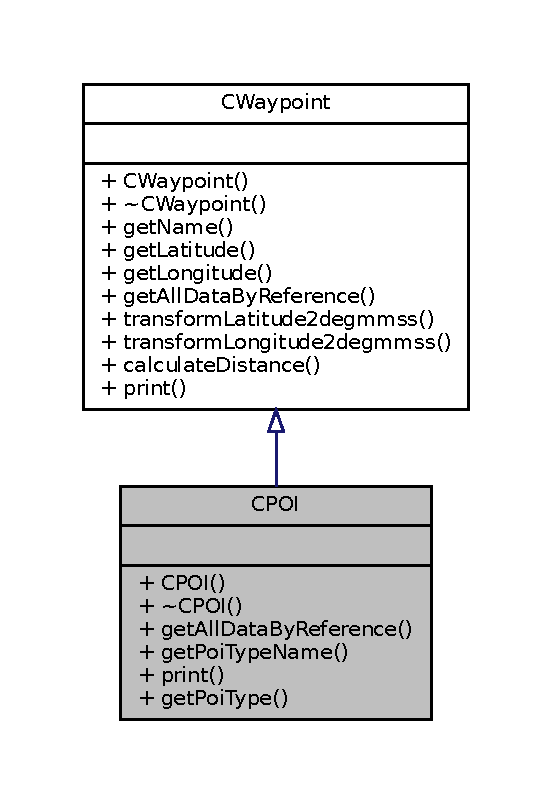
\includegraphics[width=265pt]{classCPOI__inherit__graph}
\end{center}
\end{figure}


Collaboration diagram for C\+P\+OI\+:
\nopagebreak
\begin{figure}[H]
\begin{center}
\leavevmode
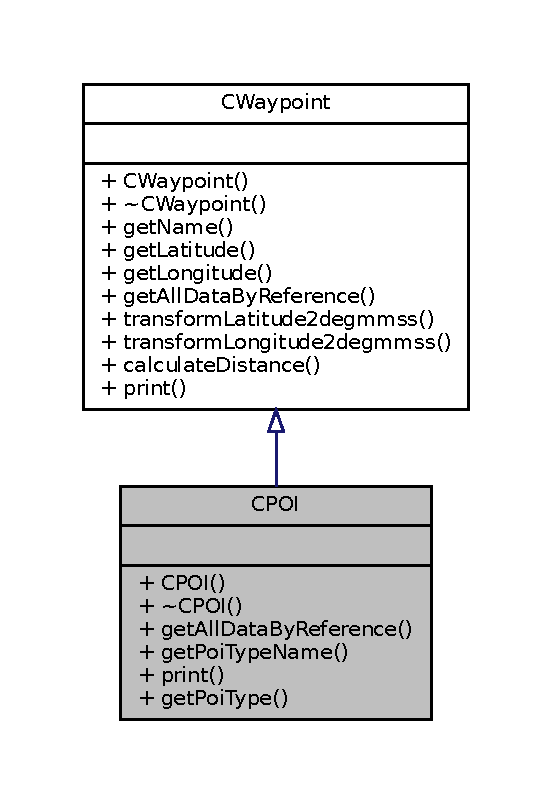
\includegraphics[width=265pt]{classCPOI__coll__graph}
\end{center}
\end{figure}
\subsection*{Public Types}
\begin{DoxyCompactItemize}
\item 
enum \hyperlink{classCPOI_a4b95e2e14055d2f9ca134e474dd4a19f}{t\+\_\+poi} \{ \newline
\hyperlink{classCPOI_a4b95e2e14055d2f9ca134e474dd4a19fa9e2e59681f7e72aecac624223b9fa8e4}{R\+E\+S\+T\+A\+U\+R\+A\+NT} = 0, 
\hyperlink{classCPOI_a4b95e2e14055d2f9ca134e474dd4a19facf4a12f93b8c022863d68afc23eba40c}{T\+O\+U\+R\+I\+S\+T\+IC}, 
\hyperlink{classCPOI_a4b95e2e14055d2f9ca134e474dd4a19faea743cce5aaba1631332753cc174e959}{G\+A\+S\+S\+T\+A\+T\+I\+ON}, 
\hyperlink{classCPOI_a4b95e2e14055d2f9ca134e474dd4a19faa5da5fd02f7ccaa7f05851cd08ad02e2}{U\+N\+I\+V\+E\+R\+S\+I\+TY}, 
\newline
\hyperlink{classCPOI_a4b95e2e14055d2f9ca134e474dd4a19fa2c7961f7a81e01841006025f0653b0f0}{D\+E\+F\+A\+U\+L\+T\+\_\+\+P\+OI}
 \}
\item 
enum \hyperlink{classCPOI_a8b2f40865be2841f714570f02cfa5308}{Attributes\+Type} \{ \newline
\hyperlink{classCPOI_a8b2f40865be2841f714570f02cfa5308a5c6f58856c64c6d4551c6d3633c5389b}{I\+N\+V\+A\+L\+I\+D\+\_\+\+T\+Y\+PE} = 0, 
\hyperlink{classCPOI_a8b2f40865be2841f714570f02cfa5308ab8e333612d4db73c33947c2388295a12}{N\+A\+ME}, 
\hyperlink{classCPOI_a8b2f40865be2841f714570f02cfa5308a57ea5a2fc969fac0404968f7791824cb}{L\+A\+T\+I\+T\+U\+DE}, 
\hyperlink{classCPOI_a8b2f40865be2841f714570f02cfa5308a2c5ae5d334f3e644260138be14e29e42}{L\+O\+N\+G\+I\+T\+U\+DE}, 
\newline
\hyperlink{classCPOI_a8b2f40865be2841f714570f02cfa5308a91fafb096c2a3f1359ce122d91526401}{P\+O\+I\+\_\+\+T\+Y\+PE}, 
\hyperlink{classCPOI_a8b2f40865be2841f714570f02cfa5308a2ff203a7d3c5fd108d72db1e2138064e}{D\+E\+S\+C\+R\+I\+P\+T\+I\+ON}, 
\hyperlink{classCPOI_a8b2f40865be2841f714570f02cfa5308a3fce19695d636371523a0ffc51ace1fc}{M\+A\+X\+\_\+\+T\+Y\+P\+ES}
 \}
\end{DoxyCompactItemize}
\subsection*{Public Member Functions}
\begin{DoxyCompactItemize}
\item 
\hyperlink{classCPOI_a9dd1c6e7b2a3e82ca3a383cc0a02bf8d}{C\+P\+OI} (\hyperlink{classCPOI_a4b95e2e14055d2f9ca134e474dd4a19f}{t\+\_\+poi} type=\hyperlink{classCPOI_a4b95e2e14055d2f9ca134e474dd4a19fa2c7961f7a81e01841006025f0653b0f0}{D\+E\+F\+A\+U\+L\+T\+\_\+\+P\+OI}, std\+::string name=\char`\"{}\char`\"{}, std\+::string description=\char`\"{}\char`\"{}, double latitude=0, double longitude=0)
\item 
\hyperlink{classCPOI_a8fc284c7b62be827e11f7e8ae443c55f}{$\sim$\+C\+P\+OI} ()
\item 
void \hyperlink{classCPOI_a65c0161ce80d49cf5f2fe80765bc94d9}{get\+All\+Data\+By\+Reference} (std\+::string \&name, double \&latitude, double \&longitude, \hyperlink{classCPOI_a4b95e2e14055d2f9ca134e474dd4a19f}{t\+\_\+poi} \&type, std\+::string \&description)
\item 
std\+::string \hyperlink{classCPOI_a908fcdd7b79aca230c67c05bf1b1a78c}{get\+Poi\+Type\+Name} ()
\item 
void \hyperlink{classCPOI_a2b65d12e722c89a8a105620726195d10}{print} (int format)
\end{DoxyCompactItemize}
\subsection*{Static Public Member Functions}
\begin{DoxyCompactItemize}
\item 
static \hyperlink{classCPOI_a4b95e2e14055d2f9ca134e474dd4a19f}{C\+P\+O\+I\+::t\+\_\+poi} \hyperlink{classCPOI_ac100f8c90fe0e5057e6fa4eca53126ad}{get\+Poi\+Type} (const std\+::string \&poi\+Type\+Name)
\end{DoxyCompactItemize}
\subsection*{Friends}
\begin{DoxyCompactItemize}
\item 
std\+::ostream \& \hyperlink{classCPOI_ad0c53792637fc266cb40d31e21c8a68f}{operator$<$$<$} (std\+::ostream \&stream, \hyperlink{classCPOI}{C\+P\+OI} const \&poi)
\end{DoxyCompactItemize}


\subsection{Member Enumeration Documentation}
\mbox{\Hypertarget{classCPOI_a8b2f40865be2841f714570f02cfa5308}\label{classCPOI_a8b2f40865be2841f714570f02cfa5308}} 
\index{C\+P\+OI@{C\+P\+OI}!Attributes\+Type@{Attributes\+Type}}
\index{Attributes\+Type@{Attributes\+Type}!C\+P\+OI@{C\+P\+OI}}
\subsubsection{\texorpdfstring{Attributes\+Type}{AttributesType}}
{\footnotesize\ttfamily enum \hyperlink{classCPOI_a8b2f40865be2841f714570f02cfa5308}{C\+P\+O\+I\+::\+Attributes\+Type}}

\begin{DoxyEnumFields}{Enumerator}
\raisebox{\heightof{T}}[0pt][0pt]{\index{I\+N\+V\+A\+L\+I\+D\+\_\+\+T\+Y\+PE@{I\+N\+V\+A\+L\+I\+D\+\_\+\+T\+Y\+PE}!C\+P\+OI@{C\+P\+OI}}\index{C\+P\+OI@{C\+P\+OI}!I\+N\+V\+A\+L\+I\+D\+\_\+\+T\+Y\+PE@{I\+N\+V\+A\+L\+I\+D\+\_\+\+T\+Y\+PE}}}\mbox{\Hypertarget{classCPOI_a8b2f40865be2841f714570f02cfa5308a5c6f58856c64c6d4551c6d3633c5389b}\label{classCPOI_a8b2f40865be2841f714570f02cfa5308a5c6f58856c64c6d4551c6d3633c5389b}} 
I\+N\+V\+A\+L\+I\+D\+\_\+\+T\+Y\+PE&\\
\hline

\raisebox{\heightof{T}}[0pt][0pt]{\index{N\+A\+ME@{N\+A\+ME}!C\+P\+OI@{C\+P\+OI}}\index{C\+P\+OI@{C\+P\+OI}!N\+A\+ME@{N\+A\+ME}}}\mbox{\Hypertarget{classCPOI_a8b2f40865be2841f714570f02cfa5308ab8e333612d4db73c33947c2388295a12}\label{classCPOI_a8b2f40865be2841f714570f02cfa5308ab8e333612d4db73c33947c2388295a12}} 
N\+A\+ME&\\
\hline

\raisebox{\heightof{T}}[0pt][0pt]{\index{L\+A\+T\+I\+T\+U\+DE@{L\+A\+T\+I\+T\+U\+DE}!C\+P\+OI@{C\+P\+OI}}\index{C\+P\+OI@{C\+P\+OI}!L\+A\+T\+I\+T\+U\+DE@{L\+A\+T\+I\+T\+U\+DE}}}\mbox{\Hypertarget{classCPOI_a8b2f40865be2841f714570f02cfa5308a57ea5a2fc969fac0404968f7791824cb}\label{classCPOI_a8b2f40865be2841f714570f02cfa5308a57ea5a2fc969fac0404968f7791824cb}} 
L\+A\+T\+I\+T\+U\+DE&\\
\hline

\raisebox{\heightof{T}}[0pt][0pt]{\index{L\+O\+N\+G\+I\+T\+U\+DE@{L\+O\+N\+G\+I\+T\+U\+DE}!C\+P\+OI@{C\+P\+OI}}\index{C\+P\+OI@{C\+P\+OI}!L\+O\+N\+G\+I\+T\+U\+DE@{L\+O\+N\+G\+I\+T\+U\+DE}}}\mbox{\Hypertarget{classCPOI_a8b2f40865be2841f714570f02cfa5308a2c5ae5d334f3e644260138be14e29e42}\label{classCPOI_a8b2f40865be2841f714570f02cfa5308a2c5ae5d334f3e644260138be14e29e42}} 
L\+O\+N\+G\+I\+T\+U\+DE&\\
\hline

\raisebox{\heightof{T}}[0pt][0pt]{\index{P\+O\+I\+\_\+\+T\+Y\+PE@{P\+O\+I\+\_\+\+T\+Y\+PE}!C\+P\+OI@{C\+P\+OI}}\index{C\+P\+OI@{C\+P\+OI}!P\+O\+I\+\_\+\+T\+Y\+PE@{P\+O\+I\+\_\+\+T\+Y\+PE}}}\mbox{\Hypertarget{classCPOI_a8b2f40865be2841f714570f02cfa5308a91fafb096c2a3f1359ce122d91526401}\label{classCPOI_a8b2f40865be2841f714570f02cfa5308a91fafb096c2a3f1359ce122d91526401}} 
P\+O\+I\+\_\+\+T\+Y\+PE&\\
\hline

\raisebox{\heightof{T}}[0pt][0pt]{\index{D\+E\+S\+C\+R\+I\+P\+T\+I\+ON@{D\+E\+S\+C\+R\+I\+P\+T\+I\+ON}!C\+P\+OI@{C\+P\+OI}}\index{C\+P\+OI@{C\+P\+OI}!D\+E\+S\+C\+R\+I\+P\+T\+I\+ON@{D\+E\+S\+C\+R\+I\+P\+T\+I\+ON}}}\mbox{\Hypertarget{classCPOI_a8b2f40865be2841f714570f02cfa5308a2ff203a7d3c5fd108d72db1e2138064e}\label{classCPOI_a8b2f40865be2841f714570f02cfa5308a2ff203a7d3c5fd108d72db1e2138064e}} 
D\+E\+S\+C\+R\+I\+P\+T\+I\+ON&\\
\hline

\raisebox{\heightof{T}}[0pt][0pt]{\index{M\+A\+X\+\_\+\+T\+Y\+P\+ES@{M\+A\+X\+\_\+\+T\+Y\+P\+ES}!C\+P\+OI@{C\+P\+OI}}\index{C\+P\+OI@{C\+P\+OI}!M\+A\+X\+\_\+\+T\+Y\+P\+ES@{M\+A\+X\+\_\+\+T\+Y\+P\+ES}}}\mbox{\Hypertarget{classCPOI_a8b2f40865be2841f714570f02cfa5308a3fce19695d636371523a0ffc51ace1fc}\label{classCPOI_a8b2f40865be2841f714570f02cfa5308a3fce19695d636371523a0ffc51ace1fc}} 
M\+A\+X\+\_\+\+T\+Y\+P\+ES&\\
\hline

\end{DoxyEnumFields}
\mbox{\Hypertarget{classCPOI_a4b95e2e14055d2f9ca134e474dd4a19f}\label{classCPOI_a4b95e2e14055d2f9ca134e474dd4a19f}} 
\index{C\+P\+OI@{C\+P\+OI}!t\+\_\+poi@{t\+\_\+poi}}
\index{t\+\_\+poi@{t\+\_\+poi}!C\+P\+OI@{C\+P\+OI}}
\subsubsection{\texorpdfstring{t\+\_\+poi}{t\_poi}}
{\footnotesize\ttfamily enum \hyperlink{classCPOI_a4b95e2e14055d2f9ca134e474dd4a19f}{C\+P\+O\+I\+::t\+\_\+poi}}

\begin{DoxyEnumFields}{Enumerator}
\raisebox{\heightof{T}}[0pt][0pt]{\index{R\+E\+S\+T\+A\+U\+R\+A\+NT@{R\+E\+S\+T\+A\+U\+R\+A\+NT}!C\+P\+OI@{C\+P\+OI}}\index{C\+P\+OI@{C\+P\+OI}!R\+E\+S\+T\+A\+U\+R\+A\+NT@{R\+E\+S\+T\+A\+U\+R\+A\+NT}}}\mbox{\Hypertarget{classCPOI_a4b95e2e14055d2f9ca134e474dd4a19fa9e2e59681f7e72aecac624223b9fa8e4}\label{classCPOI_a4b95e2e14055d2f9ca134e474dd4a19fa9e2e59681f7e72aecac624223b9fa8e4}} 
R\+E\+S\+T\+A\+U\+R\+A\+NT&\\
\hline

\raisebox{\heightof{T}}[0pt][0pt]{\index{T\+O\+U\+R\+I\+S\+T\+IC@{T\+O\+U\+R\+I\+S\+T\+IC}!C\+P\+OI@{C\+P\+OI}}\index{C\+P\+OI@{C\+P\+OI}!T\+O\+U\+R\+I\+S\+T\+IC@{T\+O\+U\+R\+I\+S\+T\+IC}}}\mbox{\Hypertarget{classCPOI_a4b95e2e14055d2f9ca134e474dd4a19facf4a12f93b8c022863d68afc23eba40c}\label{classCPOI_a4b95e2e14055d2f9ca134e474dd4a19facf4a12f93b8c022863d68afc23eba40c}} 
T\+O\+U\+R\+I\+S\+T\+IC&\\
\hline

\raisebox{\heightof{T}}[0pt][0pt]{\index{G\+A\+S\+S\+T\+A\+T\+I\+ON@{G\+A\+S\+S\+T\+A\+T\+I\+ON}!C\+P\+OI@{C\+P\+OI}}\index{C\+P\+OI@{C\+P\+OI}!G\+A\+S\+S\+T\+A\+T\+I\+ON@{G\+A\+S\+S\+T\+A\+T\+I\+ON}}}\mbox{\Hypertarget{classCPOI_a4b95e2e14055d2f9ca134e474dd4a19faea743cce5aaba1631332753cc174e959}\label{classCPOI_a4b95e2e14055d2f9ca134e474dd4a19faea743cce5aaba1631332753cc174e959}} 
G\+A\+S\+S\+T\+A\+T\+I\+ON&\\
\hline

\raisebox{\heightof{T}}[0pt][0pt]{\index{U\+N\+I\+V\+E\+R\+S\+I\+TY@{U\+N\+I\+V\+E\+R\+S\+I\+TY}!C\+P\+OI@{C\+P\+OI}}\index{C\+P\+OI@{C\+P\+OI}!U\+N\+I\+V\+E\+R\+S\+I\+TY@{U\+N\+I\+V\+E\+R\+S\+I\+TY}}}\mbox{\Hypertarget{classCPOI_a4b95e2e14055d2f9ca134e474dd4a19faa5da5fd02f7ccaa7f05851cd08ad02e2}\label{classCPOI_a4b95e2e14055d2f9ca134e474dd4a19faa5da5fd02f7ccaa7f05851cd08ad02e2}} 
U\+N\+I\+V\+E\+R\+S\+I\+TY&\\
\hline

\raisebox{\heightof{T}}[0pt][0pt]{\index{D\+E\+F\+A\+U\+L\+T\+\_\+\+P\+OI@{D\+E\+F\+A\+U\+L\+T\+\_\+\+P\+OI}!C\+P\+OI@{C\+P\+OI}}\index{C\+P\+OI@{C\+P\+OI}!D\+E\+F\+A\+U\+L\+T\+\_\+\+P\+OI@{D\+E\+F\+A\+U\+L\+T\+\_\+\+P\+OI}}}\mbox{\Hypertarget{classCPOI_a4b95e2e14055d2f9ca134e474dd4a19fa2c7961f7a81e01841006025f0653b0f0}\label{classCPOI_a4b95e2e14055d2f9ca134e474dd4a19fa2c7961f7a81e01841006025f0653b0f0}} 
D\+E\+F\+A\+U\+L\+T\+\_\+\+P\+OI&\\
\hline

\end{DoxyEnumFields}


\subsection{Constructor \& Destructor Documentation}
\mbox{\Hypertarget{classCPOI_a9dd1c6e7b2a3e82ca3a383cc0a02bf8d}\label{classCPOI_a9dd1c6e7b2a3e82ca3a383cc0a02bf8d}} 
\index{C\+P\+OI@{C\+P\+OI}!C\+P\+OI@{C\+P\+OI}}
\index{C\+P\+OI@{C\+P\+OI}!C\+P\+OI@{C\+P\+OI}}
\subsubsection{\texorpdfstring{C\+P\+O\+I()}{CPOI()}}
{\footnotesize\ttfamily C\+P\+O\+I\+::\+C\+P\+OI (\begin{DoxyParamCaption}\item[{\hyperlink{classCPOI_a4b95e2e14055d2f9ca134e474dd4a19f}{t\+\_\+poi}}]{type = {\ttfamily \hyperlink{classCPOI_a4b95e2e14055d2f9ca134e474dd4a19fa2c7961f7a81e01841006025f0653b0f0}{D\+E\+F\+A\+U\+L\+T\+\_\+\+P\+OI}},  }\item[{std\+::string}]{name = {\ttfamily \char`\"{}\char`\"{}},  }\item[{std\+::string}]{description = {\ttfamily \char`\"{}\char`\"{}},  }\item[{double}]{latitude = {\ttfamily 0},  }\item[{double}]{longitude = {\ttfamily 0} }\end{DoxyParamCaption})}

\hyperlink{classCPOI}{C\+P\+OI} constructor\+: Sets the value of an object when created. param@ t\+\_\+poi type -\/ type of a Point of interest (IN) param@ string name -\/ name of a Waypoint (IN) param@ double latitude -\/ latitude of a Waypoint (IN) param@ double longitude -\/ longitude of a Waypoint (IN) \mbox{\Hypertarget{classCPOI_a8fc284c7b62be827e11f7e8ae443c55f}\label{classCPOI_a8fc284c7b62be827e11f7e8ae443c55f}} 
\index{C\+P\+OI@{C\+P\+OI}!````~C\+P\+OI@{$\sim$\+C\+P\+OI}}
\index{````~C\+P\+OI@{$\sim$\+C\+P\+OI}!C\+P\+OI@{C\+P\+OI}}
\subsubsection{\texorpdfstring{$\sim$\+C\+P\+O\+I()}{~CPOI()}}
{\footnotesize\ttfamily C\+P\+O\+I\+::$\sim$\+C\+P\+OI (\begin{DoxyParamCaption}{ }\end{DoxyParamCaption})}

\hyperlink{classCPOI}{C\+P\+OI} Destructor\+: Called when the object is destroyed 

\subsection{Member Function Documentation}
\mbox{\Hypertarget{classCPOI_a65c0161ce80d49cf5f2fe80765bc94d9}\label{classCPOI_a65c0161ce80d49cf5f2fe80765bc94d9}} 
\index{C\+P\+OI@{C\+P\+OI}!get\+All\+Data\+By\+Reference@{get\+All\+Data\+By\+Reference}}
\index{get\+All\+Data\+By\+Reference@{get\+All\+Data\+By\+Reference}!C\+P\+OI@{C\+P\+OI}}
\subsubsection{\texorpdfstring{get\+All\+Data\+By\+Reference()}{getAllDataByReference()}}
{\footnotesize\ttfamily void C\+P\+O\+I\+::get\+All\+Data\+By\+Reference (\begin{DoxyParamCaption}\item[{std\+::string \&}]{name,  }\item[{double \&}]{latitude,  }\item[{double \&}]{longitude,  }\item[{\hyperlink{classCPOI_a4b95e2e14055d2f9ca134e474dd4a19f}{t\+\_\+poi} \&}]{type,  }\item[{std\+::string \&}]{description }\end{DoxyParamCaption})}

\mbox{\Hypertarget{classCPOI_ac100f8c90fe0e5057e6fa4eca53126ad}\label{classCPOI_ac100f8c90fe0e5057e6fa4eca53126ad}} 
\index{C\+P\+OI@{C\+P\+OI}!get\+Poi\+Type@{get\+Poi\+Type}}
\index{get\+Poi\+Type@{get\+Poi\+Type}!C\+P\+OI@{C\+P\+OI}}
\subsubsection{\texorpdfstring{get\+Poi\+Type()}{getPoiType()}}
{\footnotesize\ttfamily \hyperlink{classCPOI_a4b95e2e14055d2f9ca134e474dd4a19f}{C\+P\+O\+I\+::t\+\_\+poi} C\+P\+O\+I\+::get\+Poi\+Type (\begin{DoxyParamCaption}\item[{const std\+::string \&}]{poi\+Type\+Name }\end{DoxyParamCaption})\hspace{0.3cm}{\ttfamily [static]}}

Gets the type -\/ Global function param@ const string \&poi\+Type\+Name -\/ P\+OI name (IN) returnvalue@ \hyperlink{classCPOI_a4b95e2e14055d2f9ca134e474dd4a19f}{C\+P\+O\+I\+::t\+\_\+poi} -\/ P\+OI type

Gets the type param@ const string \&poi\+Type\+Name -\/ P\+OI name (IN) returnvalue@ \hyperlink{classCPOI_a4b95e2e14055d2f9ca134e474dd4a19f}{C\+P\+O\+I\+::t\+\_\+poi} -\/ P\+OI type \mbox{\Hypertarget{classCPOI_a908fcdd7b79aca230c67c05bf1b1a78c}\label{classCPOI_a908fcdd7b79aca230c67c05bf1b1a78c}} 
\index{C\+P\+OI@{C\+P\+OI}!get\+Poi\+Type\+Name@{get\+Poi\+Type\+Name}}
\index{get\+Poi\+Type\+Name@{get\+Poi\+Type\+Name}!C\+P\+OI@{C\+P\+OI}}
\subsubsection{\texorpdfstring{get\+Poi\+Type\+Name()}{getPoiTypeName()}}
{\footnotesize\ttfamily string C\+P\+O\+I\+::get\+Poi\+Type\+Name (\begin{DoxyParamCaption}{ }\end{DoxyParamCaption})}

Gets the type name in the string returnvalue@ string -\/ name of the P\+OI type \mbox{\Hypertarget{classCPOI_a2b65d12e722c89a8a105620726195d10}\label{classCPOI_a2b65d12e722c89a8a105620726195d10}} 
\index{C\+P\+OI@{C\+P\+OI}!print@{print}}
\index{print@{print}!C\+P\+OI@{C\+P\+OI}}
\subsubsection{\texorpdfstring{print()}{print()}}
{\footnotesize\ttfamily void C\+P\+O\+I\+::print (\begin{DoxyParamCaption}\item[{int}]{format }\end{DoxyParamCaption})\hspace{0.3cm}{\ttfamily [virtual]}}

Prints the P\+OI values in Degree-\/\+Mins-\/secs format or Decimal format param@ int format -\/ Decimal or Deg-\/min-\/ss (IN) returnvalue@ void

Prints the P\+OI values in Degree-\/\+Mins-\/secs format or Decimal format param@ int format -\/ Decimal or Deg-\/min-\/ss (O\+UT) returnvalue@ void 

Reimplemented from \hyperlink{classCWaypoint_a9a4177a2734842c9395658cb60a70c24}{C\+Waypoint}.



\subsection{Friends And Related Function Documentation}
\mbox{\Hypertarget{classCPOI_ad0c53792637fc266cb40d31e21c8a68f}\label{classCPOI_ad0c53792637fc266cb40d31e21c8a68f}} 
\index{C\+P\+OI@{C\+P\+OI}!operator$<$$<$@{operator$<$$<$}}
\index{operator$<$$<$@{operator$<$$<$}!C\+P\+OI@{C\+P\+OI}}
\subsubsection{\texorpdfstring{operator$<$$<$}{operator<<}}
{\footnotesize\ttfamily std\+::ostream\& operator$<$$<$ (\begin{DoxyParamCaption}\item[{std\+::ostream \&}]{stream,  }\item[{\hyperlink{classCPOI}{C\+P\+OI} const \&}]{poi }\end{DoxyParamCaption})\hspace{0.3cm}{\ttfamily [friend]}}

An operator overloaded friend function which prints the P\+OI information param@ ostream \&stream -\/ output stream (I\+N/\+O\+UT) param@ \hyperlink{classCPOI}{C\+P\+OI} const \&poi -\/ A P\+OI (IN) returnvalue@ output stream with the P\+OI information 

The documentation for this class was generated from the following files\+:\begin{DoxyCompactItemize}
\item 
\hyperlink{CPOI_8h}{C\+P\+O\+I.\+h}\item 
\hyperlink{CPOI_8cpp}{C\+P\+O\+I.\+cpp}\end{DoxyCompactItemize}

\hypertarget{classCPoiDatabase}{}\section{C\+Poi\+Database Class Reference}
\label{classCPoiDatabase}\index{C\+Poi\+Database@{C\+Poi\+Database}}


{\ttfamily \#include $<$C\+Poi\+Database.\+h$>$}



Inheritance diagram for C\+Poi\+Database\+:
\nopagebreak
\begin{figure}[H]
\begin{center}
\leavevmode
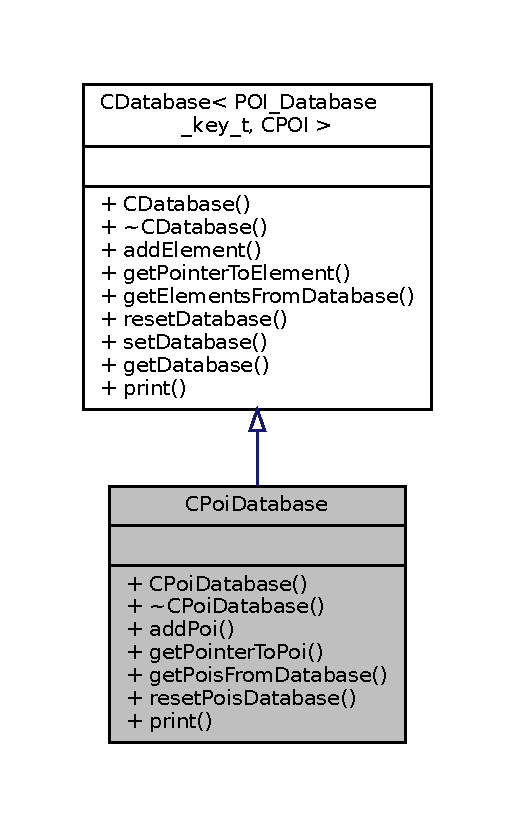
\includegraphics[width=247pt]{classCPoiDatabase__inherit__graph}
\end{center}
\end{figure}


Collaboration diagram for C\+Poi\+Database\+:
\nopagebreak
\begin{figure}[H]
\begin{center}
\leavevmode
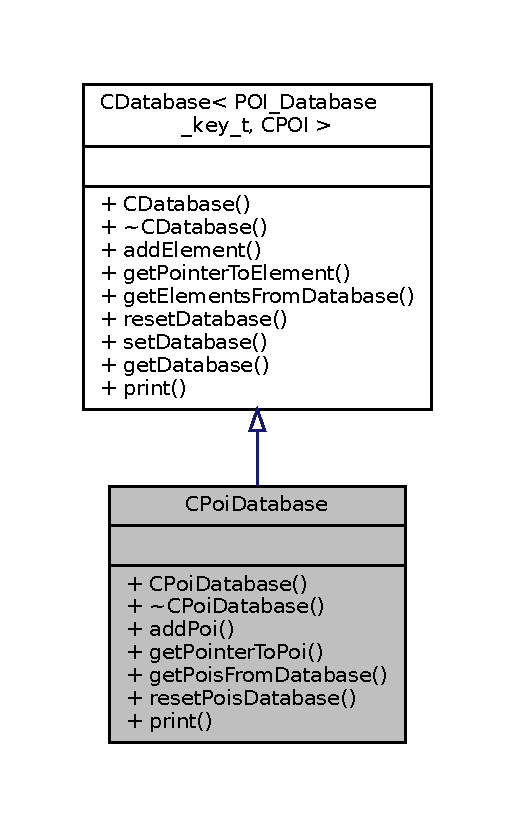
\includegraphics[width=247pt]{classCPoiDatabase__coll__graph}
\end{center}
\end{figure}
\subsection*{Public Types}
\begin{DoxyCompactItemize}
\item 
typedef std\+::map$<$ \hyperlink{CPoiDatabase_8h_ad55418fc31c1491ccfbd50da54f494a0}{P\+O\+I\+\_\+\+Database\+\_\+key\+\_\+t}, \hyperlink{classCPOI}{C\+P\+OI} $>$ \hyperlink{classCPoiDatabase_ad9ed38adc9bf4250e704cd3d378176a2}{Poi\+\_\+\+Map\+\_\+t}
\item 
typedef std\+::map$<$ \hyperlink{CPoiDatabase_8h_ad55418fc31c1491ccfbd50da54f494a0}{P\+O\+I\+\_\+\+Database\+\_\+key\+\_\+t}, \hyperlink{classCPOI}{C\+P\+OI} $>$\+::iterator \hyperlink{classCPoiDatabase_ac9ec3b0a5e8efee92521eeb03aa0b198}{Poi\+\_\+\+Map\+\_\+\+Itr\+\_\+t}
\end{DoxyCompactItemize}
\subsection*{Public Member Functions}
\begin{DoxyCompactItemize}
\item 
\hyperlink{classCPoiDatabase_a03098c79d2c4958e353658127fa0535e}{C\+Poi\+Database} ()
\item 
\hyperlink{classCPoiDatabase_a01b246bbd0dfa5bf3c94e97b09df92b2}{$\sim$\+C\+Poi\+Database} ()
\item 
void \hyperlink{classCPoiDatabase_a963761cbbaf6ad8f249d5950b428f7eb}{add\+Poi} (\hyperlink{CPoiDatabase_8h_ad55418fc31c1491ccfbd50da54f494a0}{P\+O\+I\+\_\+\+Database\+\_\+key\+\_\+t} const \&key, \hyperlink{classCPOI}{C\+P\+OI} const \&poi)
\item 
\hyperlink{classCPOI}{C\+P\+OI} $\ast$ \hyperlink{classCPoiDatabase_a4320809ce8b8f2cb6d3a9e56d598293c}{get\+Pointer\+To\+Poi} (\hyperlink{CPoiDatabase_8h_ad55418fc31c1491ccfbd50da54f494a0}{P\+O\+I\+\_\+\+Database\+\_\+key\+\_\+t} key)
\item 
const \hyperlink{classCPoiDatabase_ad9ed38adc9bf4250e704cd3d378176a2}{Poi\+\_\+\+Map\+\_\+t} \hyperlink{classCPoiDatabase_a3f5c6705e35e3f543d60fc0ddf9334a8}{get\+Pois\+From\+Database} () const
\item 
void \hyperlink{classCPoiDatabase_aab8efdfbd61515050fb1685d769cf5cd}{reset\+Pois\+Database} ()
\item 
void \hyperlink{classCPoiDatabase_a540c1119ded65c6732fc92728c5b9c14}{print} ()
\end{DoxyCompactItemize}


\subsection{Member Typedef Documentation}
\mbox{\Hypertarget{classCPoiDatabase_ac9ec3b0a5e8efee92521eeb03aa0b198}\label{classCPoiDatabase_ac9ec3b0a5e8efee92521eeb03aa0b198}} 
\index{C\+Poi\+Database@{C\+Poi\+Database}!Poi\+\_\+\+Map\+\_\+\+Itr\+\_\+t@{Poi\+\_\+\+Map\+\_\+\+Itr\+\_\+t}}
\index{Poi\+\_\+\+Map\+\_\+\+Itr\+\_\+t@{Poi\+\_\+\+Map\+\_\+\+Itr\+\_\+t}!C\+Poi\+Database@{C\+Poi\+Database}}
\subsubsection{\texorpdfstring{Poi\+\_\+\+Map\+\_\+\+Itr\+\_\+t}{Poi\_Map\_Itr\_t}}
{\footnotesize\ttfamily typedef std\+::map$<$\hyperlink{CPoiDatabase_8h_ad55418fc31c1491ccfbd50da54f494a0}{P\+O\+I\+\_\+\+Database\+\_\+key\+\_\+t}, \hyperlink{classCPOI}{C\+P\+OI}$>$\+::iterator \hyperlink{classCPoiDatabase_ac9ec3b0a5e8efee92521eeb03aa0b198}{C\+Poi\+Database\+::\+Poi\+\_\+\+Map\+\_\+\+Itr\+\_\+t}}

\mbox{\Hypertarget{classCPoiDatabase_ad9ed38adc9bf4250e704cd3d378176a2}\label{classCPoiDatabase_ad9ed38adc9bf4250e704cd3d378176a2}} 
\index{C\+Poi\+Database@{C\+Poi\+Database}!Poi\+\_\+\+Map\+\_\+t@{Poi\+\_\+\+Map\+\_\+t}}
\index{Poi\+\_\+\+Map\+\_\+t@{Poi\+\_\+\+Map\+\_\+t}!C\+Poi\+Database@{C\+Poi\+Database}}
\subsubsection{\texorpdfstring{Poi\+\_\+\+Map\+\_\+t}{Poi\_Map\_t}}
{\footnotesize\ttfamily typedef std\+::map$<$\hyperlink{CPoiDatabase_8h_ad55418fc31c1491ccfbd50da54f494a0}{P\+O\+I\+\_\+\+Database\+\_\+key\+\_\+t}, \hyperlink{classCPOI}{C\+P\+OI}$>$ \hyperlink{classCPoiDatabase_ad9ed38adc9bf4250e704cd3d378176a2}{C\+Poi\+Database\+::\+Poi\+\_\+\+Map\+\_\+t}}



\subsection{Constructor \& Destructor Documentation}
\mbox{\Hypertarget{classCPoiDatabase_a03098c79d2c4958e353658127fa0535e}\label{classCPoiDatabase_a03098c79d2c4958e353658127fa0535e}} 
\index{C\+Poi\+Database@{C\+Poi\+Database}!C\+Poi\+Database@{C\+Poi\+Database}}
\index{C\+Poi\+Database@{C\+Poi\+Database}!C\+Poi\+Database@{C\+Poi\+Database}}
\subsubsection{\texorpdfstring{C\+Poi\+Database()}{CPoiDatabase()}}
{\footnotesize\ttfamily C\+Poi\+Database\+::\+C\+Poi\+Database (\begin{DoxyParamCaption}{ }\end{DoxyParamCaption})}

\hyperlink{classCPoiDatabase}{C\+Poi\+Database} constructor \mbox{\Hypertarget{classCPoiDatabase_a01b246bbd0dfa5bf3c94e97b09df92b2}\label{classCPoiDatabase_a01b246bbd0dfa5bf3c94e97b09df92b2}} 
\index{C\+Poi\+Database@{C\+Poi\+Database}!````~C\+Poi\+Database@{$\sim$\+C\+Poi\+Database}}
\index{````~C\+Poi\+Database@{$\sim$\+C\+Poi\+Database}!C\+Poi\+Database@{C\+Poi\+Database}}
\subsubsection{\texorpdfstring{$\sim$\+C\+Poi\+Database()}{~CPoiDatabase()}}
{\footnotesize\ttfamily C\+Poi\+Database\+::$\sim$\+C\+Poi\+Database (\begin{DoxyParamCaption}{ }\end{DoxyParamCaption})}

\hyperlink{classCPoiDatabase}{C\+Poi\+Database} destructor 

\subsection{Member Function Documentation}
\mbox{\Hypertarget{classCPoiDatabase_a963761cbbaf6ad8f249d5950b428f7eb}\label{classCPoiDatabase_a963761cbbaf6ad8f249d5950b428f7eb}} 
\index{C\+Poi\+Database@{C\+Poi\+Database}!add\+Poi@{add\+Poi}}
\index{add\+Poi@{add\+Poi}!C\+Poi\+Database@{C\+Poi\+Database}}
\subsubsection{\texorpdfstring{add\+Poi()}{addPoi()}}
{\footnotesize\ttfamily void C\+Poi\+Database\+::add\+Poi (\begin{DoxyParamCaption}\item[{\hyperlink{CPoiDatabase_8h_ad55418fc31c1491ccfbd50da54f494a0}{P\+O\+I\+\_\+\+Database\+\_\+key\+\_\+t} const \&}]{key,  }\item[{\hyperlink{classCPOI}{C\+P\+OI} const \&}]{poi }\end{DoxyParamCaption})}

\mbox{\Hypertarget{classCPoiDatabase_a4320809ce8b8f2cb6d3a9e56d598293c}\label{classCPoiDatabase_a4320809ce8b8f2cb6d3a9e56d598293c}} 
\index{C\+Poi\+Database@{C\+Poi\+Database}!get\+Pointer\+To\+Poi@{get\+Pointer\+To\+Poi}}
\index{get\+Pointer\+To\+Poi@{get\+Pointer\+To\+Poi}!C\+Poi\+Database@{C\+Poi\+Database}}
\subsubsection{\texorpdfstring{get\+Pointer\+To\+Poi()}{getPointerToPoi()}}
{\footnotesize\ttfamily \hyperlink{classCPOI}{C\+P\+OI} $\ast$ C\+Poi\+Database\+::get\+Pointer\+To\+Poi (\begin{DoxyParamCaption}\item[{\hyperlink{CPoiDatabase_8h_ad55418fc31c1491ccfbd50da54f494a0}{P\+O\+I\+\_\+\+Database\+\_\+key\+\_\+t}}]{key }\end{DoxyParamCaption})}

Get pointer to a P\+OI from the Database which matches the name param@ P\+O\+I\+\_\+\+Database\+\_\+key\+\_\+t key -\/ key of a P\+OI (IN) returnvalue@ C\+P\+O\+I$\ast$ -\/ Pointer to a P\+OI in the database(\+I\+N)

Get pointer to a P\+OI from the Database which matches the name param@ string key -\/ name of a P\+OI (IN) returnvalue@ C\+P\+O\+I$\ast$ -\/ Pointer to a P\+OI in the database \mbox{\Hypertarget{classCPoiDatabase_a3f5c6705e35e3f543d60fc0ddf9334a8}\label{classCPoiDatabase_a3f5c6705e35e3f543d60fc0ddf9334a8}} 
\index{C\+Poi\+Database@{C\+Poi\+Database}!get\+Pois\+From\+Database@{get\+Pois\+From\+Database}}
\index{get\+Pois\+From\+Database@{get\+Pois\+From\+Database}!C\+Poi\+Database@{C\+Poi\+Database}}
\subsubsection{\texorpdfstring{get\+Pois\+From\+Database()}{getPoisFromDatabase()}}
{\footnotesize\ttfamily const \hyperlink{classCPoiDatabase_ad9ed38adc9bf4250e704cd3d378176a2}{C\+Poi\+Database\+::\+Poi\+\_\+\+Map\+\_\+t} C\+Poi\+Database\+::get\+Pois\+From\+Database (\begin{DoxyParamCaption}{ }\end{DoxyParamCaption}) const}

Get P\+O\+Is from the Database returnvalue@ Poi\+\_\+\+Map\+\_\+t -\/ P\+O\+Is in the Database (O\+UT) \mbox{\Hypertarget{classCPoiDatabase_a540c1119ded65c6732fc92728c5b9c14}\label{classCPoiDatabase_a540c1119ded65c6732fc92728c5b9c14}} 
\index{C\+Poi\+Database@{C\+Poi\+Database}!print@{print}}
\index{print@{print}!C\+Poi\+Database@{C\+Poi\+Database}}
\subsubsection{\texorpdfstring{print()}{print()}}
{\footnotesize\ttfamily void C\+Poi\+Database\+::print (\begin{DoxyParamCaption}{ }\end{DoxyParamCaption})}

Print all the P\+O\+Is in the database returnvalue@ void \mbox{\Hypertarget{classCPoiDatabase_aab8efdfbd61515050fb1685d769cf5cd}\label{classCPoiDatabase_aab8efdfbd61515050fb1685d769cf5cd}} 
\index{C\+Poi\+Database@{C\+Poi\+Database}!reset\+Pois\+Database@{reset\+Pois\+Database}}
\index{reset\+Pois\+Database@{reset\+Pois\+Database}!C\+Poi\+Database@{C\+Poi\+Database}}
\subsubsection{\texorpdfstring{reset\+Pois\+Database()}{resetPoisDatabase()}}
{\footnotesize\ttfamily void C\+Poi\+Database\+::reset\+Pois\+Database (\begin{DoxyParamCaption}{ }\end{DoxyParamCaption})}

Resets the Database returnvalue@ void

Reset the Database returnvalue@ void 

The documentation for this class was generated from the following files\+:\begin{DoxyCompactItemize}
\item 
\hyperlink{CPoiDatabase_8h}{C\+Poi\+Database.\+h}\item 
\hyperlink{CPoiDatabase_8cpp}{C\+Poi\+Database.\+cpp}\end{DoxyCompactItemize}

\hypertarget{classCRoute}{}\section{C\+Route Class Reference}
\label{classCRoute}\index{C\+Route@{C\+Route}}


{\ttfamily \#include $<$C\+Route.\+h$>$}



Collaboration diagram for C\+Route\+:
\nopagebreak
\begin{figure}[H]
\begin{center}
\leavevmode
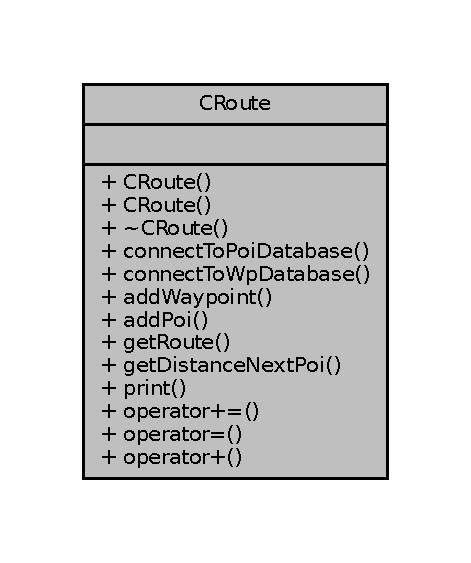
\includegraphics[width=226pt]{classCRoute__coll__graph}
\end{center}
\end{figure}
\subsection*{Public Member Functions}
\begin{DoxyCompactItemize}
\item 
\hyperlink{classCRoute_a279642bf28bce1bb9865317db93bb08b}{C\+Route} ()
\item 
\hyperlink{classCRoute_a0f6fad7298482d4717380ec91a5d0bf9}{C\+Route} (\hyperlink{classCRoute}{C\+Route} const \&origin)
\item 
\hyperlink{classCRoute_ac78e6d6f34788ee62f5d65b182cf1c2f}{$\sim$\+C\+Route} ()
\item 
void \hyperlink{classCRoute_a04173f3a28fb020f0704a0703956836f}{connect\+To\+Poi\+Database} (\hyperlink{classCPoiDatabase}{C\+Poi\+Database} $\ast$p\+Poi\+DB)
\item 
void \hyperlink{classCRoute_a0efb25d5f4c3167b189c03cbcd3d64f9}{connect\+To\+Wp\+Database} (\hyperlink{classCWpDatabase}{C\+Wp\+Database} $\ast$p\+Wp\+DB)
\item 
void \hyperlink{classCRoute_ade32420c69c3b4bb2e6068619607f279}{add\+Waypoint} (\hyperlink{CRoute_8h_a112678f2c32c39b2d50c558d89dbde68}{Database\+\_\+key\+\_\+t} key)
\item 
void \hyperlink{classCRoute_ab925dec9a729fbcad96f85065df36b61}{add\+Poi} (\hyperlink{CRoute_8h_a112678f2c32c39b2d50c558d89dbde68}{Database\+\_\+key\+\_\+t} name\+Poi, std\+::string after\+Wp)
\item 
const std\+::vector$<$ const \hyperlink{classCWaypoint}{C\+Waypoint} $\ast$ $>$ \hyperlink{classCRoute_a4e359e364950dc60f1669ff36761e716}{get\+Route} ()
\item 
double \hyperlink{classCRoute_ac0eb87d7cce83cee166de71857fa68cb}{get\+Distance\+Next\+Poi} (\hyperlink{classCWaypoint}{C\+Waypoint} const \&wp, \hyperlink{classCPOI}{C\+P\+OI} \&poi)
\item 
void \hyperlink{classCRoute_ac414ab61fe61cf703eb6225b25d9f09c}{print} ()
\item 
void \hyperlink{classCRoute_a278402d6f68b924679c555a933b6312c}{operator+=} (\hyperlink{CRoute_8h_a112678f2c32c39b2d50c558d89dbde68}{Database\+\_\+key\+\_\+t} const \&name)
\item 
\hyperlink{classCRoute}{C\+Route} \& \hyperlink{classCRoute_a898a4b296423fe629a771de487aae7fc}{operator=} (\hyperlink{classCRoute}{C\+Route} const \&rhs)
\item 
\hyperlink{classCRoute}{C\+Route} \hyperlink{classCRoute_aa9d2cdf6f3a0ce51ca4ab0c4285004a9}{operator+} (\hyperlink{classCRoute}{C\+Route} const \&rhs)
\end{DoxyCompactItemize}


\subsection{Constructor \& Destructor Documentation}
\mbox{\Hypertarget{classCRoute_a279642bf28bce1bb9865317db93bb08b}\label{classCRoute_a279642bf28bce1bb9865317db93bb08b}} 
\index{C\+Route@{C\+Route}!C\+Route@{C\+Route}}
\index{C\+Route@{C\+Route}!C\+Route@{C\+Route}}
\subsubsection{\texorpdfstring{C\+Route()}{CRoute()}\hspace{0.1cm}{\footnotesize\ttfamily [1/2]}}
{\footnotesize\ttfamily C\+Route\+::\+C\+Route (\begin{DoxyParamCaption}{ }\end{DoxyParamCaption})}

\hyperlink{classCRoute}{C\+Route} Constructor\+: Sets the value when an object is created. \mbox{\Hypertarget{classCRoute_a0f6fad7298482d4717380ec91a5d0bf9}\label{classCRoute_a0f6fad7298482d4717380ec91a5d0bf9}} 
\index{C\+Route@{C\+Route}!C\+Route@{C\+Route}}
\index{C\+Route@{C\+Route}!C\+Route@{C\+Route}}
\subsubsection{\texorpdfstring{C\+Route()}{CRoute()}\hspace{0.1cm}{\footnotesize\ttfamily [2/2]}}
{\footnotesize\ttfamily C\+Route\+::\+C\+Route (\begin{DoxyParamCaption}\item[{\hyperlink{classCRoute}{C\+Route} const \&}]{origin }\end{DoxyParamCaption})}

\hyperlink{classCRoute}{C\+Route} Constructor\+: Sets the value when an object is created by performing deep copy. 
\begin{DoxyParams}{Parameters}
{\em \hyperlink{classCRoute}{C\+Route}} & const \&origin -\/ \hyperlink{classCRoute}{C\+Route} const object (IN) \\
\hline
\end{DoxyParams}
\mbox{\Hypertarget{classCRoute_ac78e6d6f34788ee62f5d65b182cf1c2f}\label{classCRoute_ac78e6d6f34788ee62f5d65b182cf1c2f}} 
\index{C\+Route@{C\+Route}!````~C\+Route@{$\sim$\+C\+Route}}
\index{````~C\+Route@{$\sim$\+C\+Route}!C\+Route@{C\+Route}}
\subsubsection{\texorpdfstring{$\sim$\+C\+Route()}{~CRoute()}}
{\footnotesize\ttfamily C\+Route\+::$\sim$\+C\+Route (\begin{DoxyParamCaption}{ }\end{DoxyParamCaption})}

\hyperlink{classCRoute}{C\+Route} Destructor\+: Called when the object is destroyed

\hyperlink{classCRoute}{C\+Route} Destructor 

\subsection{Member Function Documentation}
\mbox{\Hypertarget{classCRoute_ab925dec9a729fbcad96f85065df36b61}\label{classCRoute_ab925dec9a729fbcad96f85065df36b61}} 
\index{C\+Route@{C\+Route}!add\+Poi@{add\+Poi}}
\index{add\+Poi@{add\+Poi}!C\+Route@{C\+Route}}
\subsubsection{\texorpdfstring{add\+Poi()}{addPoi()}}
{\footnotesize\ttfamily void C\+Route\+::add\+Poi (\begin{DoxyParamCaption}\item[{\hyperlink{CRoute_8h_a112678f2c32c39b2d50c558d89dbde68}{Database\+\_\+key\+\_\+t}}]{name\+Poi,  }\item[{std\+::string}]{after\+Wp }\end{DoxyParamCaption})}

Search the P\+OI in the P\+O\+I-\/database by the name; Add the P\+OI to current route after \char`\"{}after\+Wp\char`\"{} 
\begin{DoxyParams}{Parameters}
{\em Database\+\_\+key\+\_\+t} & name\+Poi -\/ name of a P\+OI (IN) \\
\hline
{\em string} & after\+Wp -\/ name of a waypoint(\+I\+N)  void\\
\hline
\end{DoxyParams}
Search the P\+OI in the P\+O\+I-\/database by the name; Add the P\+OI to current route after \char`\"{}after\+Wp\char`\"{} if -\/$>$ name\+Poi is empty and after\+Wp is empty -\/$>$ don\textquotesingle{}t add name\+Poi is empty and after\+Wp is not empty -\/$>$ P\+OI will not be in the DB name\+Poi is not empty and after\+Wp is empty -\/$>$ Add P\+OI to Route at the end name\+Poi is not empty and after\+Wp is not empty -\/$>$ Add P\+OI after\+Wp where after\+WP is already added


\begin{DoxyParams}{Parameters}
{\em Database\+\_\+key\+\_\+t} & name\+Poi -\/ name of a P\+OI (IN) \\
\hline
{\em string} & after\+Wp -\/ name of a waypoint(\+I\+N)  void \\
\hline
\end{DoxyParams}
\mbox{\Hypertarget{classCRoute_ade32420c69c3b4bb2e6068619607f279}\label{classCRoute_ade32420c69c3b4bb2e6068619607f279}} 
\index{C\+Route@{C\+Route}!add\+Waypoint@{add\+Waypoint}}
\index{add\+Waypoint@{add\+Waypoint}!C\+Route@{C\+Route}}
\subsubsection{\texorpdfstring{add\+Waypoint()}{addWaypoint()}}
{\footnotesize\ttfamily void C\+Route\+::add\+Waypoint (\begin{DoxyParamCaption}\item[{\hyperlink{CRoute_8h_a112678f2c32c39b2d50c558d89dbde68}{Database\+\_\+key\+\_\+t}}]{key }\end{DoxyParamCaption})}

Search the waypoint in the waypoint-\/database by the name; Add the waypoint to current route 
\begin{DoxyParams}{Parameters}
{\em Database\+\_\+key\+\_\+t} & key -\/ name of a waypoint (IN)  void \\
\hline
\end{DoxyParams}
\mbox{\Hypertarget{classCRoute_a04173f3a28fb020f0704a0703956836f}\label{classCRoute_a04173f3a28fb020f0704a0703956836f}} 
\index{C\+Route@{C\+Route}!connect\+To\+Poi\+Database@{connect\+To\+Poi\+Database}}
\index{connect\+To\+Poi\+Database@{connect\+To\+Poi\+Database}!C\+Route@{C\+Route}}
\subsubsection{\texorpdfstring{connect\+To\+Poi\+Database()}{connectToPoiDatabase()}}
{\footnotesize\ttfamily void C\+Route\+::connect\+To\+Poi\+Database (\begin{DoxyParamCaption}\item[{\hyperlink{classCPoiDatabase}{C\+Poi\+Database} $\ast$}]{p\+Poi\+DB }\end{DoxyParamCaption})}

Get the address of the P\+OI Database and connect it to the \hyperlink{classCRoute}{C\+Route} 
\begin{DoxyParams}{Parameters}
{\em C\+Poi\+Database$\ast$} & p\+Poi\+DB -\/ pointer to the P\+OI Database (IN)  void \\
\hline
\end{DoxyParams}
\mbox{\Hypertarget{classCRoute_a0efb25d5f4c3167b189c03cbcd3d64f9}\label{classCRoute_a0efb25d5f4c3167b189c03cbcd3d64f9}} 
\index{C\+Route@{C\+Route}!connect\+To\+Wp\+Database@{connect\+To\+Wp\+Database}}
\index{connect\+To\+Wp\+Database@{connect\+To\+Wp\+Database}!C\+Route@{C\+Route}}
\subsubsection{\texorpdfstring{connect\+To\+Wp\+Database()}{connectToWpDatabase()}}
{\footnotesize\ttfamily void C\+Route\+::connect\+To\+Wp\+Database (\begin{DoxyParamCaption}\item[{\hyperlink{classCWpDatabase}{C\+Wp\+Database} $\ast$}]{p\+Wp\+DB }\end{DoxyParamCaption})}

Get the address of the Waypoint Database and connect it to the \hyperlink{classCRoute}{C\+Route} 
\begin{DoxyParams}{Parameters}
{\em \hyperlink{classCWpDatabase}{C\+Wp\+Database}} & $\ast$p\+Wp\+DB -\/ pointer to the Waypoint Database (IN)  void \\
\hline
\end{DoxyParams}
\mbox{\Hypertarget{classCRoute_ac0eb87d7cce83cee166de71857fa68cb}\label{classCRoute_ac0eb87d7cce83cee166de71857fa68cb}} 
\index{C\+Route@{C\+Route}!get\+Distance\+Next\+Poi@{get\+Distance\+Next\+Poi}}
\index{get\+Distance\+Next\+Poi@{get\+Distance\+Next\+Poi}!C\+Route@{C\+Route}}
\subsubsection{\texorpdfstring{get\+Distance\+Next\+Poi()}{getDistanceNextPoi()}}
{\footnotesize\ttfamily double C\+Route\+::get\+Distance\+Next\+Poi (\begin{DoxyParamCaption}\item[{\hyperlink{classCWaypoint}{C\+Waypoint} const \&}]{wp,  }\item[{\hyperlink{classCPOI}{C\+P\+OI} \&}]{poi }\end{DoxyParamCaption})}

Calculates the distance between waypoint and P\+OI 
\begin{DoxyParams}{Parameters}
{\em \hyperlink{classCWaypoint}{C\+Waypoint}} & const \&wp -\/ waypoint (IN) \\
\hline
{\em C\+P\+O\+I\&} & poi -\/ P\+OI (IN) \\
\hline
\end{DoxyParams}
\begin{DoxyReturn}{Returns}
double -\/ Distance in Kms 
\end{DoxyReturn}
\mbox{\Hypertarget{classCRoute_a4e359e364950dc60f1669ff36761e716}\label{classCRoute_a4e359e364950dc60f1669ff36761e716}} 
\index{C\+Route@{C\+Route}!get\+Route@{get\+Route}}
\index{get\+Route@{get\+Route}!C\+Route@{C\+Route}}
\subsubsection{\texorpdfstring{get\+Route()}{getRoute()}}
{\footnotesize\ttfamily const vector$<$ const \hyperlink{classCWaypoint}{C\+Waypoint} $\ast$ $>$ C\+Route\+::get\+Route (\begin{DoxyParamCaption}{ }\end{DoxyParamCaption})}

Get the current route information  vector -\/ Current route having Waypoints and P\+OI \mbox{\Hypertarget{classCRoute_aa9d2cdf6f3a0ce51ca4ab0c4285004a9}\label{classCRoute_aa9d2cdf6f3a0ce51ca4ab0c4285004a9}} 
\index{C\+Route@{C\+Route}!operator+@{operator+}}
\index{operator+@{operator+}!C\+Route@{C\+Route}}
\subsubsection{\texorpdfstring{operator+()}{operator+()}}
{\footnotesize\ttfamily \hyperlink{classCRoute}{C\+Route} C\+Route\+::operator+ (\begin{DoxyParamCaption}\item[{\hyperlink{classCRoute}{C\+Route} const \&}]{rhs }\end{DoxyParamCaption})}

An addition operator 
\begin{DoxyParams}{Parameters}
{\em \hyperlink{classCRoute}{C\+Route}} & const \& rhs -\/ \hyperlink{classCRoute}{C\+Route} const object (IN)  \hyperlink{classCRoute}{C\+Route} \\
\hline
\end{DoxyParams}
\mbox{\Hypertarget{classCRoute_a278402d6f68b924679c555a933b6312c}\label{classCRoute_a278402d6f68b924679c555a933b6312c}} 
\index{C\+Route@{C\+Route}!operator+=@{operator+=}}
\index{operator+=@{operator+=}!C\+Route@{C\+Route}}
\subsubsection{\texorpdfstring{operator+=()}{operator+=()}}
{\footnotesize\ttfamily void C\+Route\+::operator+= (\begin{DoxyParamCaption}\item[{\hyperlink{CRoute_8h_a112678f2c32c39b2d50c558d89dbde68}{Database\+\_\+key\+\_\+t} const \&}]{name }\end{DoxyParamCaption})}

The function is an extension of add\+Poi which searches the Databases and add the Waypoint or the P\+OI which matches the name.

The function is an extension of add\+Poi which searches the Databases and add the Waypoint and/or the P\+OI which matches the name. \mbox{\Hypertarget{classCRoute_a898a4b296423fe629a771de487aae7fc}\label{classCRoute_a898a4b296423fe629a771de487aae7fc}} 
\index{C\+Route@{C\+Route}!operator=@{operator=}}
\index{operator=@{operator=}!C\+Route@{C\+Route}}
\subsubsection{\texorpdfstring{operator=()}{operator=()}}
{\footnotesize\ttfamily \hyperlink{classCRoute}{C\+Route} \& C\+Route\+::operator= (\begin{DoxyParamCaption}\item[{\hyperlink{classCRoute}{C\+Route} const \&}]{rhs }\end{DoxyParamCaption})}

A copy assignment operator 
\begin{DoxyParams}{Parameters}
{\em \hyperlink{classCRoute}{C\+Route}} & const \& rhs -\/ \hyperlink{classCRoute}{C\+Route} const object (IN)  \hyperlink{classCRoute}{C\+Route}\& \\
\hline
\end{DoxyParams}
\mbox{\Hypertarget{classCRoute_ac414ab61fe61cf703eb6225b25d9f09c}\label{classCRoute_ac414ab61fe61cf703eb6225b25d9f09c}} 
\index{C\+Route@{C\+Route}!print@{print}}
\index{print@{print}!C\+Route@{C\+Route}}
\subsubsection{\texorpdfstring{print()}{print()}}
{\footnotesize\ttfamily void C\+Route\+::print (\begin{DoxyParamCaption}{ }\end{DoxyParamCaption})}

prints all the waypoints and P\+O\+Is in the route 

The documentation for this class was generated from the following files\+:\begin{DoxyCompactItemize}
\item 
\hyperlink{CRoute_8h}{C\+Route.\+h}\item 
\hyperlink{CRoute_8cpp}{C\+Route.\+cpp}\end{DoxyCompactItemize}

\hypertarget{classCWaypoint}{}\section{C\+Waypoint Class Reference}
\label{classCWaypoint}\index{C\+Waypoint@{C\+Waypoint}}


{\ttfamily \#include $<$C\+Waypoint.\+h$>$}



Inheritance diagram for C\+Waypoint\+:
\nopagebreak
\begin{figure}[H]
\begin{center}
\leavevmode
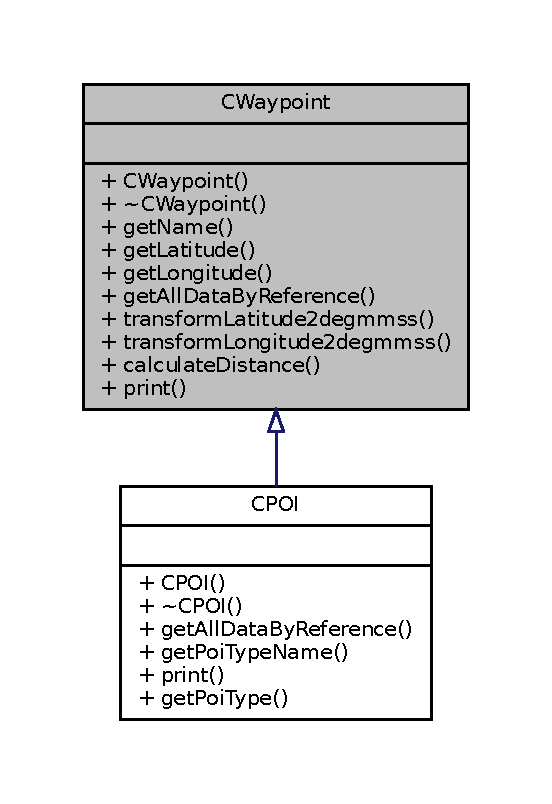
\includegraphics[width=265pt]{classCWaypoint__inherit__graph}
\end{center}
\end{figure}


Collaboration diagram for C\+Waypoint\+:
\nopagebreak
\begin{figure}[H]
\begin{center}
\leavevmode
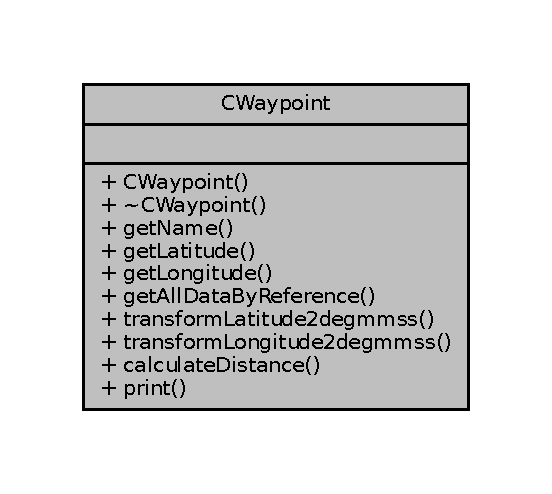
\includegraphics[width=265pt]{classCWaypoint__coll__graph}
\end{center}
\end{figure}
\subsection*{Public Types}
\begin{DoxyCompactItemize}
\item 
enum \hyperlink{classCWaypoint_afc0d93011dc8399f17e05ea26f1abb8a}{wp\+\_\+type} \{ \hyperlink{classCWaypoint_afc0d93011dc8399f17e05ea26f1abb8aa22c9bb710a20488e41e0522f836edcee}{W\+A\+Y\+P\+O\+I\+NT}, 
\hyperlink{classCWaypoint_afc0d93011dc8399f17e05ea26f1abb8aac5313b10832538160cae4612688df59f}{P\+OI}, 
\hyperlink{classCWaypoint_afc0d93011dc8399f17e05ea26f1abb8aaf3998ae68619b810a26451138606a57e}{I\+N\+V\+A\+L\+ID}
 \}
\end{DoxyCompactItemize}
\subsection*{Public Member Functions}
\begin{DoxyCompactItemize}
\item 
\hyperlink{classCWaypoint_addbb5ff027b48242d3e905ccfb7c6453}{C\+Waypoint} (std\+::string name=\char`\"{}\char`\"{}, double latitude=0, double longitude=0, \hyperlink{classCWaypoint_afc0d93011dc8399f17e05ea26f1abb8a}{wp\+\_\+type} type=\hyperlink{classCWaypoint_afc0d93011dc8399f17e05ea26f1abb8aa22c9bb710a20488e41e0522f836edcee}{W\+A\+Y\+P\+O\+I\+NT})
\item 
virtual \hyperlink{classCWaypoint_a74c7197b95df5dc4e631935d33c5ad27}{$\sim$\+C\+Waypoint} ()
\item 
std\+::string \hyperlink{classCWaypoint_afa0887a7523a345624046168fe3a2ce5}{get\+Name} () const
\item 
double \hyperlink{classCWaypoint_a8040d28d7b4628799f61565ba53e55b0}{get\+Latitude} ()
\item 
double \hyperlink{classCWaypoint_a662b4705b3f60929856ebacdebf8bf2d}{get\+Longitude} ()
\item 
void \hyperlink{classCWaypoint_a352acef38557203e1e266528e2aa23cf}{get\+All\+Data\+By\+Reference} (std\+::string \&name, double \&latitude, double \&longitude)
\item 
void \hyperlink{classCWaypoint_aec530aa8f453abd22cf41d8a6c6080f2}{transform\+Latitude2degmmss} (int \&deg, int \&mm, double \&ss)
\item 
void \hyperlink{classCWaypoint_aba26f2ba294cf5bb5bd0be1d9fdb1214}{transform\+Longitude2degmmss} (int \&deg, int \&mm, double \&ss)
\item 
double \hyperlink{classCWaypoint_aff44ab2fb23c9b96646550392644dd8a}{calculate\+Distance} (const \hyperlink{classCWaypoint}{C\+Waypoint} \&wp)
\item 
virtual void \hyperlink{classCWaypoint_a9a4177a2734842c9395658cb60a70c24}{print} (int format)
\end{DoxyCompactItemize}
\subsection*{Friends}
\begin{DoxyCompactItemize}
\item 
std\+::ostream \& \hyperlink{classCWaypoint_a7403a96c1fcf3263e880835cb4590cde}{operator$<$$<$} (std\+::ostream \&stream, \hyperlink{classCWaypoint}{C\+Waypoint} const \&wp)
\end{DoxyCompactItemize}


\subsection{Member Enumeration Documentation}
\mbox{\Hypertarget{classCWaypoint_afc0d93011dc8399f17e05ea26f1abb8a}\label{classCWaypoint_afc0d93011dc8399f17e05ea26f1abb8a}} 
\index{C\+Waypoint@{C\+Waypoint}!wp\+\_\+type@{wp\+\_\+type}}
\index{wp\+\_\+type@{wp\+\_\+type}!C\+Waypoint@{C\+Waypoint}}
\subsubsection{\texorpdfstring{wp\+\_\+type}{wp\_type}}
{\footnotesize\ttfamily enum \hyperlink{classCWaypoint_afc0d93011dc8399f17e05ea26f1abb8a}{C\+Waypoint\+::wp\+\_\+type}}

\begin{DoxyEnumFields}{Enumerator}
\raisebox{\heightof{T}}[0pt][0pt]{\index{W\+A\+Y\+P\+O\+I\+NT@{W\+A\+Y\+P\+O\+I\+NT}!C\+Waypoint@{C\+Waypoint}}\index{C\+Waypoint@{C\+Waypoint}!W\+A\+Y\+P\+O\+I\+NT@{W\+A\+Y\+P\+O\+I\+NT}}}\mbox{\Hypertarget{classCWaypoint_afc0d93011dc8399f17e05ea26f1abb8aa22c9bb710a20488e41e0522f836edcee}\label{classCWaypoint_afc0d93011dc8399f17e05ea26f1abb8aa22c9bb710a20488e41e0522f836edcee}} 
W\+A\+Y\+P\+O\+I\+NT&\\
\hline

\raisebox{\heightof{T}}[0pt][0pt]{\index{P\+OI@{P\+OI}!C\+Waypoint@{C\+Waypoint}}\index{C\+Waypoint@{C\+Waypoint}!P\+OI@{P\+OI}}}\mbox{\Hypertarget{classCWaypoint_afc0d93011dc8399f17e05ea26f1abb8aac5313b10832538160cae4612688df59f}\label{classCWaypoint_afc0d93011dc8399f17e05ea26f1abb8aac5313b10832538160cae4612688df59f}} 
P\+OI&\\
\hline

\raisebox{\heightof{T}}[0pt][0pt]{\index{I\+N\+V\+A\+L\+ID@{I\+N\+V\+A\+L\+ID}!C\+Waypoint@{C\+Waypoint}}\index{C\+Waypoint@{C\+Waypoint}!I\+N\+V\+A\+L\+ID@{I\+N\+V\+A\+L\+ID}}}\mbox{\Hypertarget{classCWaypoint_afc0d93011dc8399f17e05ea26f1abb8aaf3998ae68619b810a26451138606a57e}\label{classCWaypoint_afc0d93011dc8399f17e05ea26f1abb8aaf3998ae68619b810a26451138606a57e}} 
I\+N\+V\+A\+L\+ID&\\
\hline

\end{DoxyEnumFields}


\subsection{Constructor \& Destructor Documentation}
\mbox{\Hypertarget{classCWaypoint_addbb5ff027b48242d3e905ccfb7c6453}\label{classCWaypoint_addbb5ff027b48242d3e905ccfb7c6453}} 
\index{C\+Waypoint@{C\+Waypoint}!C\+Waypoint@{C\+Waypoint}}
\index{C\+Waypoint@{C\+Waypoint}!C\+Waypoint@{C\+Waypoint}}
\subsubsection{\texorpdfstring{C\+Waypoint()}{CWaypoint()}}
{\footnotesize\ttfamily C\+Waypoint\+::\+C\+Waypoint (\begin{DoxyParamCaption}\item[{std\+::string}]{name = {\ttfamily \char`\"{}\char`\"{}},  }\item[{double}]{latitude = {\ttfamily 0},  }\item[{double}]{longitude = {\ttfamily 0},  }\item[{\hyperlink{classCWaypoint_afc0d93011dc8399f17e05ea26f1abb8a}{wp\+\_\+type}}]{type = {\ttfamily \hyperlink{classCWaypoint_afc0d93011dc8399f17e05ea26f1abb8aa22c9bb710a20488e41e0522f836edcee}{W\+A\+Y\+P\+O\+I\+NT}} }\end{DoxyParamCaption})}

\hyperlink{classCWaypoint}{C\+Waypoint} constructor\+: Sets the value of an object when created. param@ string name -\/ name of a Waypoint, default value \char`\"{}\char`\"{} (IN) param@ double latitude -\/ latitude of a Waypoint, default value 0 (IN) param@ double longitude -\/ longitude of a Waypoint,default value 0 (IN) param@ wp\+\_\+type type -\/ Type of data -\/ P\+OI / Waypoint, default invalid (IN)

\hyperlink{classCWaypoint}{C\+Waypoint} constructor\+: Sets the value of any object when created param@ string name -\/ name of a Waypoint (IN) param@ double latitude -\/ latitude of a Waypoint (IN) param@ double longitude -\/ longitude of a Waypoint (IN) param@ wp\+\_\+type type -\/ type of data the object represents\+: P\+OI / Waypoint / Invalid(\+I\+N) \mbox{\Hypertarget{classCWaypoint_a74c7197b95df5dc4e631935d33c5ad27}\label{classCWaypoint_a74c7197b95df5dc4e631935d33c5ad27}} 
\index{C\+Waypoint@{C\+Waypoint}!````~C\+Waypoint@{$\sim$\+C\+Waypoint}}
\index{````~C\+Waypoint@{$\sim$\+C\+Waypoint}!C\+Waypoint@{C\+Waypoint}}
\subsubsection{\texorpdfstring{$\sim$\+C\+Waypoint()}{~CWaypoint()}}
{\footnotesize\ttfamily C\+Waypoint\+::$\sim$\+C\+Waypoint (\begin{DoxyParamCaption}{ }\end{DoxyParamCaption})\hspace{0.3cm}{\ttfamily [virtual]}}

Destructor 

\subsection{Member Function Documentation}
\mbox{\Hypertarget{classCWaypoint_aff44ab2fb23c9b96646550392644dd8a}\label{classCWaypoint_aff44ab2fb23c9b96646550392644dd8a}} 
\index{C\+Waypoint@{C\+Waypoint}!calculate\+Distance@{calculate\+Distance}}
\index{calculate\+Distance@{calculate\+Distance}!C\+Waypoint@{C\+Waypoint}}
\subsubsection{\texorpdfstring{calculate\+Distance()}{calculateDistance()}}
{\footnotesize\ttfamily double C\+Waypoint\+::calculate\+Distance (\begin{DoxyParamCaption}\item[{const \hyperlink{classCWaypoint}{C\+Waypoint} \&}]{wp }\end{DoxyParamCaption})}

Return the distance between 2 waypoint co-\/ordinates param@ const \hyperlink{classCWaypoint}{C\+Waypoint}\& wp -\/ Waypoint co-\/ordinate (IN) returnvalue@ double -\/ Distance in K\+Ms \mbox{\Hypertarget{classCWaypoint_a352acef38557203e1e266528e2aa23cf}\label{classCWaypoint_a352acef38557203e1e266528e2aa23cf}} 
\index{C\+Waypoint@{C\+Waypoint}!get\+All\+Data\+By\+Reference@{get\+All\+Data\+By\+Reference}}
\index{get\+All\+Data\+By\+Reference@{get\+All\+Data\+By\+Reference}!C\+Waypoint@{C\+Waypoint}}
\subsubsection{\texorpdfstring{get\+All\+Data\+By\+Reference()}{getAllDataByReference()}}
{\footnotesize\ttfamily void C\+Waypoint\+::get\+All\+Data\+By\+Reference (\begin{DoxyParamCaption}\item[{std\+::string \&}]{name,  }\item[{double \&}]{latitude,  }\item[{double \&}]{longitude }\end{DoxyParamCaption})}

Return the current waypoint co-\/ordinate values param@ string\& name -\/ name of a Waypoint (O\+UT) param@ double\& latitude -\/ latitude of a Waypoint (O\+UT) param@ double\& longitude -\/ longitude of a Waypoint (O\+UT) returnvalue@ void \mbox{\Hypertarget{classCWaypoint_a8040d28d7b4628799f61565ba53e55b0}\label{classCWaypoint_a8040d28d7b4628799f61565ba53e55b0}} 
\index{C\+Waypoint@{C\+Waypoint}!get\+Latitude@{get\+Latitude}}
\index{get\+Latitude@{get\+Latitude}!C\+Waypoint@{C\+Waypoint}}
\subsubsection{\texorpdfstring{get\+Latitude()}{getLatitude()}}
{\footnotesize\ttfamily double C\+Waypoint\+::get\+Latitude (\begin{DoxyParamCaption}{ }\end{DoxyParamCaption})}

Return the current waypoint latitude returnvalue@ double latitude -\/ latitude of a Waypoint \mbox{\Hypertarget{classCWaypoint_a662b4705b3f60929856ebacdebf8bf2d}\label{classCWaypoint_a662b4705b3f60929856ebacdebf8bf2d}} 
\index{C\+Waypoint@{C\+Waypoint}!get\+Longitude@{get\+Longitude}}
\index{get\+Longitude@{get\+Longitude}!C\+Waypoint@{C\+Waypoint}}
\subsubsection{\texorpdfstring{get\+Longitude()}{getLongitude()}}
{\footnotesize\ttfamily double C\+Waypoint\+::get\+Longitude (\begin{DoxyParamCaption}{ }\end{DoxyParamCaption})}

Return the current waypoint longitude returnvalue@ double longitude-\/ longitude of a Waypoint \mbox{\Hypertarget{classCWaypoint_afa0887a7523a345624046168fe3a2ce5}\label{classCWaypoint_afa0887a7523a345624046168fe3a2ce5}} 
\index{C\+Waypoint@{C\+Waypoint}!get\+Name@{get\+Name}}
\index{get\+Name@{get\+Name}!C\+Waypoint@{C\+Waypoint}}
\subsubsection{\texorpdfstring{get\+Name()}{getName()}}
{\footnotesize\ttfamily string C\+Waypoint\+::get\+Name (\begin{DoxyParamCaption}{ }\end{DoxyParamCaption}) const}

Return the current waypoint co-\/ordinate name retuvalue@ string name -\/ name of a Waypoint \mbox{\Hypertarget{classCWaypoint_a9a4177a2734842c9395658cb60a70c24}\label{classCWaypoint_a9a4177a2734842c9395658cb60a70c24}} 
\index{C\+Waypoint@{C\+Waypoint}!print@{print}}
\index{print@{print}!C\+Waypoint@{C\+Waypoint}}
\subsubsection{\texorpdfstring{print()}{print()}}
{\footnotesize\ttfamily void C\+Waypoint\+::print (\begin{DoxyParamCaption}\item[{int}]{format }\end{DoxyParamCaption})\hspace{0.3cm}{\ttfamily [virtual]}}

Prints the waypoint values in Degree-\/\+Mins-\/secs format or Decimal format param@ int format -\/ Decimal or Deg-\/min-\/ss (O\+UT) returnvalue@ void

Prints the waypoint values in Degree-\/\+Mins-\/secs format or Decimal format returnvalue@ void 

Reimplemented in \hyperlink{classCPOI_a2b65d12e722c89a8a105620726195d10}{C\+P\+OI}.

\mbox{\Hypertarget{classCWaypoint_aec530aa8f453abd22cf41d8a6c6080f2}\label{classCWaypoint_aec530aa8f453abd22cf41d8a6c6080f2}} 
\index{C\+Waypoint@{C\+Waypoint}!transform\+Latitude2degmmss@{transform\+Latitude2degmmss}}
\index{transform\+Latitude2degmmss@{transform\+Latitude2degmmss}!C\+Waypoint@{C\+Waypoint}}
\subsubsection{\texorpdfstring{transform\+Latitude2degmmss()}{transformLatitude2degmmss()}}
{\footnotesize\ttfamily void C\+Waypoint\+::transform\+Latitude2degmmss (\begin{DoxyParamCaption}\item[{int \&}]{deg,  }\item[{int \&}]{mm,  }\item[{double \&}]{ss }\end{DoxyParamCaption})}

Converts the Latitude in decimal to deg-\/min-\/sec format param@ int\& deg -\/ latitude in degrees (O\+UT) param@ int\& deg -\/ latitude in minutes (O\+UT) param@ double\& ss -\/ latitude in seconds (O\+UT) returnvalue@ void \mbox{\Hypertarget{classCWaypoint_aba26f2ba294cf5bb5bd0be1d9fdb1214}\label{classCWaypoint_aba26f2ba294cf5bb5bd0be1d9fdb1214}} 
\index{C\+Waypoint@{C\+Waypoint}!transform\+Longitude2degmmss@{transform\+Longitude2degmmss}}
\index{transform\+Longitude2degmmss@{transform\+Longitude2degmmss}!C\+Waypoint@{C\+Waypoint}}
\subsubsection{\texorpdfstring{transform\+Longitude2degmmss()}{transformLongitude2degmmss()}}
{\footnotesize\ttfamily void C\+Waypoint\+::transform\+Longitude2degmmss (\begin{DoxyParamCaption}\item[{int \&}]{deg,  }\item[{int \&}]{mm,  }\item[{double \&}]{ss }\end{DoxyParamCaption})}

Converts the Longitude in decimal to deg-\/min-\/sec format param@ int\& deg -\/ longitude in degrees (O\+UT) param@ int\& deg -\/ longitude in minutes (O\+UT) param@ double\& ss -\/ longitude in seconds (O\+UT) returnvalue@ void 

\subsection{Friends And Related Function Documentation}
\mbox{\Hypertarget{classCWaypoint_a7403a96c1fcf3263e880835cb4590cde}\label{classCWaypoint_a7403a96c1fcf3263e880835cb4590cde}} 
\index{C\+Waypoint@{C\+Waypoint}!operator$<$$<$@{operator$<$$<$}}
\index{operator$<$$<$@{operator$<$$<$}!C\+Waypoint@{C\+Waypoint}}
\subsubsection{\texorpdfstring{operator$<$$<$}{operator<<}}
{\footnotesize\ttfamily std\+::ostream\& operator$<$$<$ (\begin{DoxyParamCaption}\item[{std\+::ostream \&}]{stream,  }\item[{\hyperlink{classCWaypoint}{C\+Waypoint} const \&}]{wp }\end{DoxyParamCaption})\hspace{0.3cm}{\ttfamily [friend]}}

An operator overloaded friend function which prints the waypoint information param@ ostream \&stream -\/ output stream (I\+N/\+O\+UT) param@ \hyperlink{classCWaypoint}{C\+Waypoint} const \&wp -\/ A Waypoint (IN) returnvalue@ output stream with the waypoint information 

The documentation for this class was generated from the following files\+:\begin{DoxyCompactItemize}
\item 
\hyperlink{CWaypoint_8h}{C\+Waypoint.\+h}\item 
\hyperlink{CWaypoint_8cpp}{C\+Waypoint.\+cpp}\end{DoxyCompactItemize}

\hypertarget{classCWpDatabase}{}\section{C\+Wp\+Database Class Reference}
\label{classCWpDatabase}\index{C\+Wp\+Database@{C\+Wp\+Database}}


{\ttfamily \#include $<$C\+Wp\+Database.\+h$>$}



Inheritance diagram for C\+Wp\+Database\+:
\nopagebreak
\begin{figure}[H]
\begin{center}
\leavevmode
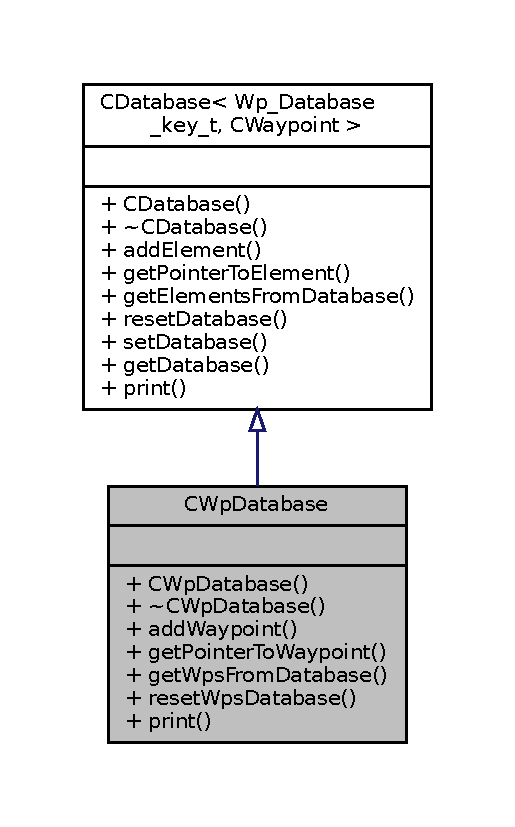
\includegraphics[width=247pt]{classCWpDatabase__inherit__graph}
\end{center}
\end{figure}


Collaboration diagram for C\+Wp\+Database\+:
\nopagebreak
\begin{figure}[H]
\begin{center}
\leavevmode
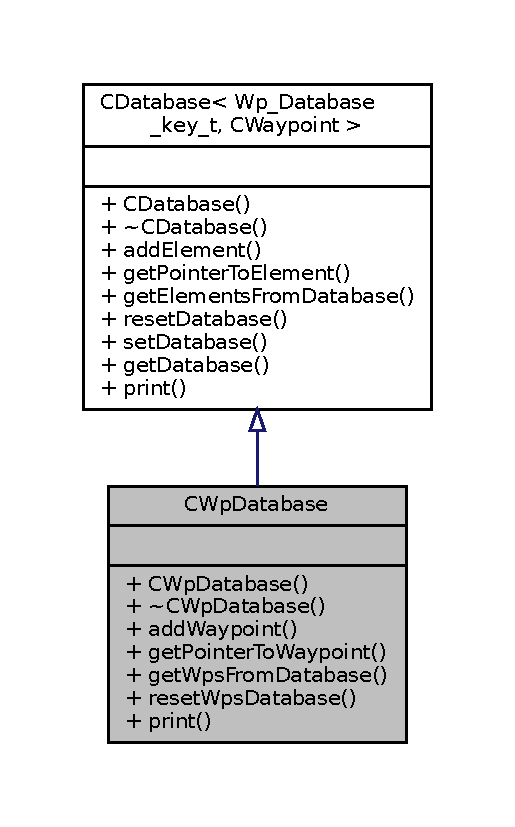
\includegraphics[width=247pt]{classCWpDatabase__coll__graph}
\end{center}
\end{figure}
\subsection*{Public Types}
\begin{DoxyCompactItemize}
\item 
typedef std\+::map$<$ \hyperlink{CWpDatabase_8h_af4bde7780fd7a000e6647ae788fe5a10}{Wp\+\_\+\+Database\+\_\+key\+\_\+t}, \hyperlink{classCWaypoint}{C\+Waypoint} $>$ \hyperlink{classCWpDatabase_acdf43fd8206955eeb54807e9254958cb}{Wp\+\_\+\+Map\+\_\+t}
\item 
typedef std\+::map$<$ \hyperlink{CWpDatabase_8h_af4bde7780fd7a000e6647ae788fe5a10}{Wp\+\_\+\+Database\+\_\+key\+\_\+t}, \hyperlink{classCWaypoint}{C\+Waypoint} $>$\+::iterator \hyperlink{classCWpDatabase_a3fbf501fb525f4f45171e7811596fc10}{Wp\+\_\+\+Map\+\_\+\+Itr\+\_\+t}
\item 
typedef std\+::map$<$ \hyperlink{CWpDatabase_8h_af4bde7780fd7a000e6647ae788fe5a10}{Wp\+\_\+\+Database\+\_\+key\+\_\+t}, \hyperlink{classCWaypoint}{C\+Waypoint} $>$\+::reverse\+\_\+iterator \hyperlink{classCWpDatabase_ae28984b70adcf73331968295206fba5d}{Wp\+\_\+\+Map\+\_\+\+Rev\+Itr\+\_\+t}
\end{DoxyCompactItemize}
\subsection*{Public Member Functions}
\begin{DoxyCompactItemize}
\item 
\hyperlink{classCWpDatabase_a373c0ba6b4524115cda152273a713017}{C\+Wp\+Database} ()
\item 
\hyperlink{classCWpDatabase_a9c8209e9d6ba9a4c275cb4f6266950d6}{$\sim$\+C\+Wp\+Database} ()
\item 
void \hyperlink{classCWpDatabase_a96d64308fe52f48b423d7c97f9e95dcf}{add\+Waypoint} (\hyperlink{CWpDatabase_8h_af4bde7780fd7a000e6647ae788fe5a10}{Wp\+\_\+\+Database\+\_\+key\+\_\+t} const \&name, \hyperlink{classCWaypoint}{C\+Waypoint} const \&wp)
\item 
\hyperlink{classCWaypoint}{C\+Waypoint} $\ast$ \hyperlink{classCWpDatabase_a5e7031a38c729dc54ff48834e2a7902f}{get\+Pointer\+To\+Waypoint} (\hyperlink{CWpDatabase_8h_af4bde7780fd7a000e6647ae788fe5a10}{Wp\+\_\+\+Database\+\_\+key\+\_\+t} name)
\item 
const \hyperlink{classCWpDatabase_acdf43fd8206955eeb54807e9254958cb}{Wp\+\_\+\+Map\+\_\+t} \hyperlink{classCWpDatabase_ad264883102664dde8c25fa8f11e41087}{get\+Wps\+From\+Database} () const
\item 
void \hyperlink{classCWpDatabase_a13e513a40e9339ae56f1c8b77eb0b9d3}{reset\+Wps\+Database} ()
\item 
void \hyperlink{classCWpDatabase_a14ca531b56bffb1dc354c5a688115d74}{print} ()
\end{DoxyCompactItemize}


\subsection{Member Typedef Documentation}
\mbox{\Hypertarget{classCWpDatabase_a3fbf501fb525f4f45171e7811596fc10}\label{classCWpDatabase_a3fbf501fb525f4f45171e7811596fc10}} 
\index{C\+Wp\+Database@{C\+Wp\+Database}!Wp\+\_\+\+Map\+\_\+\+Itr\+\_\+t@{Wp\+\_\+\+Map\+\_\+\+Itr\+\_\+t}}
\index{Wp\+\_\+\+Map\+\_\+\+Itr\+\_\+t@{Wp\+\_\+\+Map\+\_\+\+Itr\+\_\+t}!C\+Wp\+Database@{C\+Wp\+Database}}
\subsubsection{\texorpdfstring{Wp\+\_\+\+Map\+\_\+\+Itr\+\_\+t}{Wp\_Map\_Itr\_t}}
{\footnotesize\ttfamily typedef std\+::map$<$\hyperlink{CWpDatabase_8h_af4bde7780fd7a000e6647ae788fe5a10}{Wp\+\_\+\+Database\+\_\+key\+\_\+t}, \hyperlink{classCWaypoint}{C\+Waypoint}$>$\+::iterator \hyperlink{classCWpDatabase_a3fbf501fb525f4f45171e7811596fc10}{C\+Wp\+Database\+::\+Wp\+\_\+\+Map\+\_\+\+Itr\+\_\+t}}

\mbox{\Hypertarget{classCWpDatabase_ae28984b70adcf73331968295206fba5d}\label{classCWpDatabase_ae28984b70adcf73331968295206fba5d}} 
\index{C\+Wp\+Database@{C\+Wp\+Database}!Wp\+\_\+\+Map\+\_\+\+Rev\+Itr\+\_\+t@{Wp\+\_\+\+Map\+\_\+\+Rev\+Itr\+\_\+t}}
\index{Wp\+\_\+\+Map\+\_\+\+Rev\+Itr\+\_\+t@{Wp\+\_\+\+Map\+\_\+\+Rev\+Itr\+\_\+t}!C\+Wp\+Database@{C\+Wp\+Database}}
\subsubsection{\texorpdfstring{Wp\+\_\+\+Map\+\_\+\+Rev\+Itr\+\_\+t}{Wp\_Map\_RevItr\_t}}
{\footnotesize\ttfamily typedef std\+::map$<$\hyperlink{CWpDatabase_8h_af4bde7780fd7a000e6647ae788fe5a10}{Wp\+\_\+\+Database\+\_\+key\+\_\+t}, \hyperlink{classCWaypoint}{C\+Waypoint}$>$\+::reverse\+\_\+iterator \hyperlink{classCWpDatabase_ae28984b70adcf73331968295206fba5d}{C\+Wp\+Database\+::\+Wp\+\_\+\+Map\+\_\+\+Rev\+Itr\+\_\+t}}

\mbox{\Hypertarget{classCWpDatabase_acdf43fd8206955eeb54807e9254958cb}\label{classCWpDatabase_acdf43fd8206955eeb54807e9254958cb}} 
\index{C\+Wp\+Database@{C\+Wp\+Database}!Wp\+\_\+\+Map\+\_\+t@{Wp\+\_\+\+Map\+\_\+t}}
\index{Wp\+\_\+\+Map\+\_\+t@{Wp\+\_\+\+Map\+\_\+t}!C\+Wp\+Database@{C\+Wp\+Database}}
\subsubsection{\texorpdfstring{Wp\+\_\+\+Map\+\_\+t}{Wp\_Map\_t}}
{\footnotesize\ttfamily typedef std\+::map$<$\hyperlink{CWpDatabase_8h_af4bde7780fd7a000e6647ae788fe5a10}{Wp\+\_\+\+Database\+\_\+key\+\_\+t}, \hyperlink{classCWaypoint}{C\+Waypoint}$>$ \hyperlink{classCWpDatabase_acdf43fd8206955eeb54807e9254958cb}{C\+Wp\+Database\+::\+Wp\+\_\+\+Map\+\_\+t}}



\subsection{Constructor \& Destructor Documentation}
\mbox{\Hypertarget{classCWpDatabase_a373c0ba6b4524115cda152273a713017}\label{classCWpDatabase_a373c0ba6b4524115cda152273a713017}} 
\index{C\+Wp\+Database@{C\+Wp\+Database}!C\+Wp\+Database@{C\+Wp\+Database}}
\index{C\+Wp\+Database@{C\+Wp\+Database}!C\+Wp\+Database@{C\+Wp\+Database}}
\subsubsection{\texorpdfstring{C\+Wp\+Database()}{CWpDatabase()}}
{\footnotesize\ttfamily C\+Wp\+Database\+::\+C\+Wp\+Database (\begin{DoxyParamCaption}{ }\end{DoxyParamCaption})}

\hyperlink{classCWpDatabase}{C\+Wp\+Database} constructor \mbox{\Hypertarget{classCWpDatabase_a9c8209e9d6ba9a4c275cb4f6266950d6}\label{classCWpDatabase_a9c8209e9d6ba9a4c275cb4f6266950d6}} 
\index{C\+Wp\+Database@{C\+Wp\+Database}!````~C\+Wp\+Database@{$\sim$\+C\+Wp\+Database}}
\index{````~C\+Wp\+Database@{$\sim$\+C\+Wp\+Database}!C\+Wp\+Database@{C\+Wp\+Database}}
\subsubsection{\texorpdfstring{$\sim$\+C\+Wp\+Database()}{~CWpDatabase()}}
{\footnotesize\ttfamily C\+Wp\+Database\+::$\sim$\+C\+Wp\+Database (\begin{DoxyParamCaption}{ }\end{DoxyParamCaption})}

\hyperlink{classCWpDatabase}{C\+Wp\+Database} destructor 

\subsection{Member Function Documentation}
\mbox{\Hypertarget{classCWpDatabase_a96d64308fe52f48b423d7c97f9e95dcf}\label{classCWpDatabase_a96d64308fe52f48b423d7c97f9e95dcf}} 
\index{C\+Wp\+Database@{C\+Wp\+Database}!add\+Waypoint@{add\+Waypoint}}
\index{add\+Waypoint@{add\+Waypoint}!C\+Wp\+Database@{C\+Wp\+Database}}
\subsubsection{\texorpdfstring{add\+Waypoint()}{addWaypoint()}}
{\footnotesize\ttfamily void C\+Wp\+Database\+::add\+Waypoint (\begin{DoxyParamCaption}\item[{\hyperlink{CWpDatabase_8h_af4bde7780fd7a000e6647ae788fe5a10}{Wp\+\_\+\+Database\+\_\+key\+\_\+t} const \&}]{key,  }\item[{\hyperlink{classCWaypoint}{C\+Waypoint} const \&}]{wp }\end{DoxyParamCaption})}

Add a Waypoint to the database param@ Wp\+\_\+\+Database\+\_\+key\+\_\+t \&name -\/ unique name for the wp (IN) param@ \hyperlink{classCWaypoint}{C\+Waypoint} const \&wp -\/ Waypoint (IN) returnvalue@ void

Add a Waypoint to the database param@ Wp\+\_\+\+Database\+\_\+key\+\_\+t const \&key -\/ key for the wp (IN) param@ \hyperlink{classCWaypoint}{C\+Waypoint} const \&wp -\/ Waypoint (IN) returnvalue@ void \mbox{\Hypertarget{classCWpDatabase_a5e7031a38c729dc54ff48834e2a7902f}\label{classCWpDatabase_a5e7031a38c729dc54ff48834e2a7902f}} 
\index{C\+Wp\+Database@{C\+Wp\+Database}!get\+Pointer\+To\+Waypoint@{get\+Pointer\+To\+Waypoint}}
\index{get\+Pointer\+To\+Waypoint@{get\+Pointer\+To\+Waypoint}!C\+Wp\+Database@{C\+Wp\+Database}}
\subsubsection{\texorpdfstring{get\+Pointer\+To\+Waypoint()}{getPointerToWaypoint()}}
{\footnotesize\ttfamily \hyperlink{classCWaypoint}{C\+Waypoint} $\ast$ C\+Wp\+Database\+::get\+Pointer\+To\+Waypoint (\begin{DoxyParamCaption}\item[{\hyperlink{CWpDatabase_8h_af4bde7780fd7a000e6647ae788fe5a10}{Wp\+\_\+\+Database\+\_\+key\+\_\+t}}]{name }\end{DoxyParamCaption})}

Get pointer to a Waypoint from the Database which matches the name param@ Wp\+\_\+\+Database\+\_\+key\+\_\+t name -\/ name of a Waypoint (IN) returnvalue@ C\+Waypoint$\ast$ -\/ Pointer to a Waypoint in the database

Get pointer to a Waypoint from the Database which matches the name param@ Wp\+\_\+\+Database\+\_\+key\+\_\+t name -\/ name of a Waypoint (IN) returnvalue@ C\+P\+O\+I$\ast$ -\/ Pointer to a Waypoint in the database \mbox{\Hypertarget{classCWpDatabase_ad264883102664dde8c25fa8f11e41087}\label{classCWpDatabase_ad264883102664dde8c25fa8f11e41087}} 
\index{C\+Wp\+Database@{C\+Wp\+Database}!get\+Wps\+From\+Database@{get\+Wps\+From\+Database}}
\index{get\+Wps\+From\+Database@{get\+Wps\+From\+Database}!C\+Wp\+Database@{C\+Wp\+Database}}
\subsubsection{\texorpdfstring{get\+Wps\+From\+Database()}{getWpsFromDatabase()}}
{\footnotesize\ttfamily const \hyperlink{classCWpDatabase_acdf43fd8206955eeb54807e9254958cb}{C\+Wp\+Database\+::\+Wp\+\_\+\+Map\+\_\+t} C\+Wp\+Database\+::get\+Wps\+From\+Database (\begin{DoxyParamCaption}{ }\end{DoxyParamCaption}) const}

Get Waypoints from the Database returnvalue@ Wp\+\_\+\+Map\+\_\+t -\/ Waypoints in the Database (O\+UT) \mbox{\Hypertarget{classCWpDatabase_a14ca531b56bffb1dc354c5a688115d74}\label{classCWpDatabase_a14ca531b56bffb1dc354c5a688115d74}} 
\index{C\+Wp\+Database@{C\+Wp\+Database}!print@{print}}
\index{print@{print}!C\+Wp\+Database@{C\+Wp\+Database}}
\subsubsection{\texorpdfstring{print()}{print()}}
{\footnotesize\ttfamily void C\+Wp\+Database\+::print (\begin{DoxyParamCaption}{ }\end{DoxyParamCaption})}

Print all the Waypoints in the database returnvalue@ void \mbox{\Hypertarget{classCWpDatabase_a13e513a40e9339ae56f1c8b77eb0b9d3}\label{classCWpDatabase_a13e513a40e9339ae56f1c8b77eb0b9d3}} 
\index{C\+Wp\+Database@{C\+Wp\+Database}!reset\+Wps\+Database@{reset\+Wps\+Database}}
\index{reset\+Wps\+Database@{reset\+Wps\+Database}!C\+Wp\+Database@{C\+Wp\+Database}}
\subsubsection{\texorpdfstring{reset\+Wps\+Database()}{resetWpsDatabase()}}
{\footnotesize\ttfamily void C\+Wp\+Database\+::reset\+Wps\+Database (\begin{DoxyParamCaption}{ }\end{DoxyParamCaption})}

Resets the Database returnvalue@ void

Reset the Database returnvalue@ void 

The documentation for this class was generated from the following files\+:\begin{DoxyCompactItemize}
\item 
\hyperlink{CWpDatabase_8h}{C\+Wp\+Database.\+h}\item 
\hyperlink{CWpDatabase_8cpp}{C\+Wp\+Database.\+cpp}\end{DoxyCompactItemize}

\hypertarget{classFlexLexer}{}\section{Flex\+Lexer Class Reference}
\label{classFlexLexer}\index{Flex\+Lexer@{Flex\+Lexer}}


{\ttfamily \#include $<$Flex\+Lexer.\+h$>$}



Inheritance diagram for Flex\+Lexer\+:
\nopagebreak
\begin{figure}[H]
\begin{center}
\leavevmode
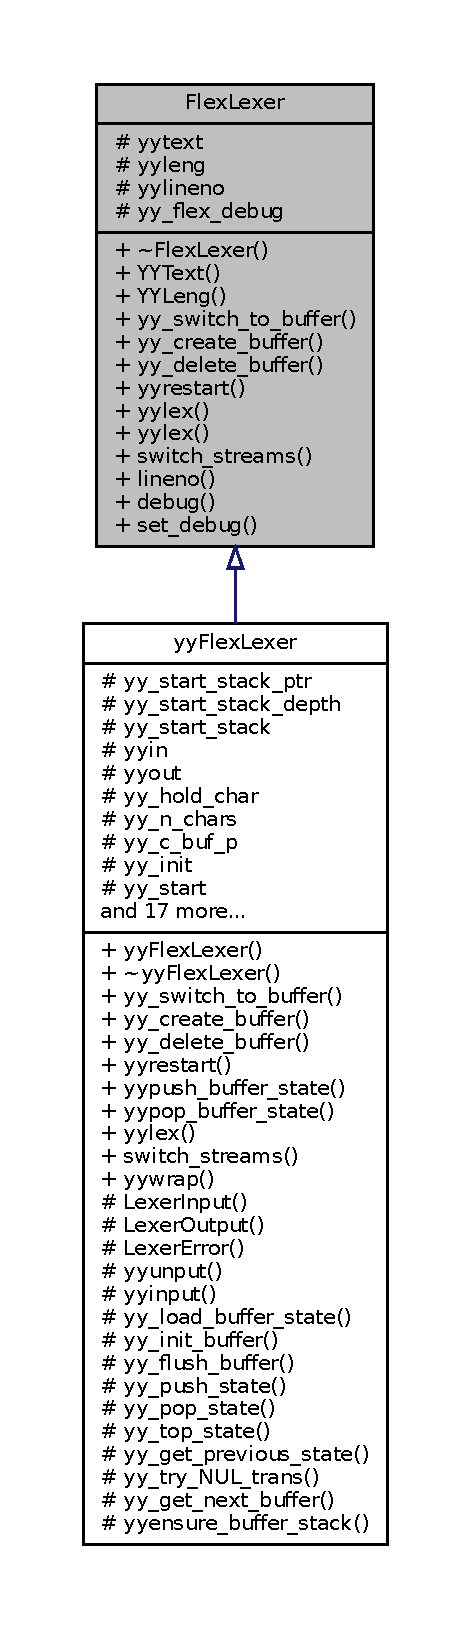
\includegraphics[height=550pt]{classFlexLexer__inherit__graph}
\end{center}
\end{figure}


Collaboration diagram for Flex\+Lexer\+:
\nopagebreak
\begin{figure}[H]
\begin{center}
\leavevmode
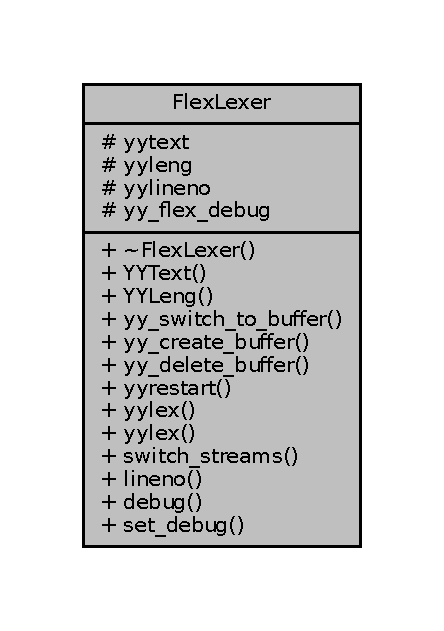
\includegraphics[width=213pt]{classFlexLexer__coll__graph}
\end{center}
\end{figure}
\subsection*{Public Member Functions}
\begin{DoxyCompactItemize}
\item 
virtual \hyperlink{classFlexLexer_a513c4982ef52db6d43151becbf3fe05a}{$\sim$\+Flex\+Lexer} ()
\item 
const char $\ast$ \hyperlink{classFlexLexer_aefb1ea757e0e455ae229ae099b4240c2}{Y\+Y\+Text} () const
\item 
int \hyperlink{classFlexLexer_aad615c6bce162fcc98c07d69371f6117}{Y\+Y\+Leng} () const
\item 
virtual void \hyperlink{classFlexLexer_a3fa4649c1866a483fc391923ca90ca1d}{yy\+\_\+switch\+\_\+to\+\_\+buffer} (struct \hyperlink{structyy__buffer__state}{yy\+\_\+buffer\+\_\+state} $\ast$new\+\_\+buffer)=0
\item 
virtual struct \hyperlink{structyy__buffer__state}{yy\+\_\+buffer\+\_\+state} $\ast$ \hyperlink{classFlexLexer_a9e0d5e33726e0270b241a730a3028990}{yy\+\_\+create\+\_\+buffer} (\hyperlink{FlexLexer_8h_ae50ff830f34b9e244163babb41a1552d}{F\+L\+E\+X\+\_\+\+S\+TD} istream $\ast$s, int size)=0
\item 
virtual void \hyperlink{classFlexLexer_a6c59180ab84ba98af3704ba2cb018230}{yy\+\_\+delete\+\_\+buffer} (struct \hyperlink{structyy__buffer__state}{yy\+\_\+buffer\+\_\+state} $\ast$b)=0
\item 
virtual void \hyperlink{classFlexLexer_a15aea8e169874756674e4f79553e68ed}{yyrestart} (\hyperlink{FlexLexer_8h_ae50ff830f34b9e244163babb41a1552d}{F\+L\+E\+X\+\_\+\+S\+TD} istream $\ast$s)=0
\item 
virtual int \hyperlink{classFlexLexer_a1b1f93d24f5a97f50eb1747fac568ccb}{yylex} ()=0
\item 
int \hyperlink{classFlexLexer_a5ec7f8b71a9cd9142963f0d924ddaa7c}{yylex} (\hyperlink{FlexLexer_8h_ae50ff830f34b9e244163babb41a1552d}{F\+L\+E\+X\+\_\+\+S\+TD} istream $\ast$new\+\_\+in, \hyperlink{FlexLexer_8h_ae50ff830f34b9e244163babb41a1552d}{F\+L\+E\+X\+\_\+\+S\+TD} ostream $\ast$new\+\_\+out=0)
\item 
virtual void \hyperlink{classFlexLexer_a09dd0826a8540365a74c2167795bbc61}{switch\+\_\+streams} (\hyperlink{FlexLexer_8h_ae50ff830f34b9e244163babb41a1552d}{F\+L\+E\+X\+\_\+\+S\+TD} istream $\ast$new\+\_\+in=0, \hyperlink{FlexLexer_8h_ae50ff830f34b9e244163babb41a1552d}{F\+L\+E\+X\+\_\+\+S\+TD} ostream $\ast$new\+\_\+out=0)=0
\item 
int \hyperlink{classFlexLexer_a835d3243729ffa4912949ea44b241f3b}{lineno} () const
\item 
int \hyperlink{classFlexLexer_a71d0a4ad9db57c86b44e84c407eb21f1}{debug} () const
\item 
void \hyperlink{classFlexLexer_a1da05b19b783fd94e8a65cb4ee02dec8}{set\+\_\+debug} (int flag)
\end{DoxyCompactItemize}
\subsection*{Protected Attributes}
\begin{DoxyCompactItemize}
\item 
char $\ast$ \hyperlink{classFlexLexer_a31e594872cba4bb896011d3ee1f75f0d}{yytext}
\item 
int \hyperlink{classFlexLexer_a7a483b8c8426cace921d961cd9634c8b}{yyleng}
\item 
int \hyperlink{classFlexLexer_a511f8fed6925478cb9925edce88024c7}{yylineno}
\item 
int \hyperlink{classFlexLexer_afb25c8701977e6f510799f4cf8a4a029}{yy\+\_\+flex\+\_\+debug}
\end{DoxyCompactItemize}


\subsection{Constructor \& Destructor Documentation}
\mbox{\Hypertarget{classFlexLexer_a513c4982ef52db6d43151becbf3fe05a}\label{classFlexLexer_a513c4982ef52db6d43151becbf3fe05a}} 
\index{Flex\+Lexer@{Flex\+Lexer}!````~Flex\+Lexer@{$\sim$\+Flex\+Lexer}}
\index{````~Flex\+Lexer@{$\sim$\+Flex\+Lexer}!Flex\+Lexer@{Flex\+Lexer}}
\subsubsection{\texorpdfstring{$\sim$\+Flex\+Lexer()}{~FlexLexer()}}
{\footnotesize\ttfamily virtual Flex\+Lexer\+::$\sim$\+Flex\+Lexer (\begin{DoxyParamCaption}{ }\end{DoxyParamCaption})\hspace{0.3cm}{\ttfamily [inline]}, {\ttfamily [virtual]}}



\subsection{Member Function Documentation}
\mbox{\Hypertarget{classFlexLexer_a71d0a4ad9db57c86b44e84c407eb21f1}\label{classFlexLexer_a71d0a4ad9db57c86b44e84c407eb21f1}} 
\index{Flex\+Lexer@{Flex\+Lexer}!debug@{debug}}
\index{debug@{debug}!Flex\+Lexer@{Flex\+Lexer}}
\subsubsection{\texorpdfstring{debug()}{debug()}}
{\footnotesize\ttfamily int Flex\+Lexer\+::debug (\begin{DoxyParamCaption}{ }\end{DoxyParamCaption}) const\hspace{0.3cm}{\ttfamily [inline]}}

\mbox{\Hypertarget{classFlexLexer_a835d3243729ffa4912949ea44b241f3b}\label{classFlexLexer_a835d3243729ffa4912949ea44b241f3b}} 
\index{Flex\+Lexer@{Flex\+Lexer}!lineno@{lineno}}
\index{lineno@{lineno}!Flex\+Lexer@{Flex\+Lexer}}
\subsubsection{\texorpdfstring{lineno()}{lineno()}}
{\footnotesize\ttfamily int Flex\+Lexer\+::lineno (\begin{DoxyParamCaption}{ }\end{DoxyParamCaption}) const\hspace{0.3cm}{\ttfamily [inline]}}

\mbox{\Hypertarget{classFlexLexer_a1da05b19b783fd94e8a65cb4ee02dec8}\label{classFlexLexer_a1da05b19b783fd94e8a65cb4ee02dec8}} 
\index{Flex\+Lexer@{Flex\+Lexer}!set\+\_\+debug@{set\+\_\+debug}}
\index{set\+\_\+debug@{set\+\_\+debug}!Flex\+Lexer@{Flex\+Lexer}}
\subsubsection{\texorpdfstring{set\+\_\+debug()}{set\_debug()}}
{\footnotesize\ttfamily void Flex\+Lexer\+::set\+\_\+debug (\begin{DoxyParamCaption}\item[{int}]{flag }\end{DoxyParamCaption})\hspace{0.3cm}{\ttfamily [inline]}}

\mbox{\Hypertarget{classFlexLexer_a09dd0826a8540365a74c2167795bbc61}\label{classFlexLexer_a09dd0826a8540365a74c2167795bbc61}} 
\index{Flex\+Lexer@{Flex\+Lexer}!switch\+\_\+streams@{switch\+\_\+streams}}
\index{switch\+\_\+streams@{switch\+\_\+streams}!Flex\+Lexer@{Flex\+Lexer}}
\subsubsection{\texorpdfstring{switch\+\_\+streams()}{switch\_streams()}}
{\footnotesize\ttfamily virtual void Flex\+Lexer\+::switch\+\_\+streams (\begin{DoxyParamCaption}\item[{\hyperlink{FlexLexer_8h_ae50ff830f34b9e244163babb41a1552d}{F\+L\+E\+X\+\_\+\+S\+TD} istream $\ast$}]{new\+\_\+in = {\ttfamily 0},  }\item[{\hyperlink{FlexLexer_8h_ae50ff830f34b9e244163babb41a1552d}{F\+L\+E\+X\+\_\+\+S\+TD} ostream $\ast$}]{new\+\_\+out = {\ttfamily 0} }\end{DoxyParamCaption})\hspace{0.3cm}{\ttfamily [pure virtual]}}



Implemented in \hyperlink{classyyFlexLexer_ae88d47b620670ef7a924f4fe1e70774b}{yy\+Flex\+Lexer}.

\mbox{\Hypertarget{classFlexLexer_a9e0d5e33726e0270b241a730a3028990}\label{classFlexLexer_a9e0d5e33726e0270b241a730a3028990}} 
\index{Flex\+Lexer@{Flex\+Lexer}!yy\+\_\+create\+\_\+buffer@{yy\+\_\+create\+\_\+buffer}}
\index{yy\+\_\+create\+\_\+buffer@{yy\+\_\+create\+\_\+buffer}!Flex\+Lexer@{Flex\+Lexer}}
\subsubsection{\texorpdfstring{yy\+\_\+create\+\_\+buffer()}{yy\_create\_buffer()}}
{\footnotesize\ttfamily virtual struct \hyperlink{structyy__buffer__state}{yy\+\_\+buffer\+\_\+state}$\ast$ Flex\+Lexer\+::yy\+\_\+create\+\_\+buffer (\begin{DoxyParamCaption}\item[{\hyperlink{FlexLexer_8h_ae50ff830f34b9e244163babb41a1552d}{F\+L\+E\+X\+\_\+\+S\+TD} istream $\ast$}]{s,  }\item[{int}]{size }\end{DoxyParamCaption})\hspace{0.3cm}{\ttfamily [pure virtual]}}



Implemented in \hyperlink{classyyFlexLexer_ac72d57010353577c918e72eba3d8972a}{yy\+Flex\+Lexer}.

\mbox{\Hypertarget{classFlexLexer_a6c59180ab84ba98af3704ba2cb018230}\label{classFlexLexer_a6c59180ab84ba98af3704ba2cb018230}} 
\index{Flex\+Lexer@{Flex\+Lexer}!yy\+\_\+delete\+\_\+buffer@{yy\+\_\+delete\+\_\+buffer}}
\index{yy\+\_\+delete\+\_\+buffer@{yy\+\_\+delete\+\_\+buffer}!Flex\+Lexer@{Flex\+Lexer}}
\subsubsection{\texorpdfstring{yy\+\_\+delete\+\_\+buffer()}{yy\_delete\_buffer()}}
{\footnotesize\ttfamily virtual void Flex\+Lexer\+::yy\+\_\+delete\+\_\+buffer (\begin{DoxyParamCaption}\item[{struct \hyperlink{structyy__buffer__state}{yy\+\_\+buffer\+\_\+state} $\ast$}]{b }\end{DoxyParamCaption})\hspace{0.3cm}{\ttfamily [pure virtual]}}



Implemented in \hyperlink{classyyFlexLexer_a645a8ebb5b2b5b80707d053a0eb7a21a}{yy\+Flex\+Lexer}.

\mbox{\Hypertarget{classFlexLexer_a3fa4649c1866a483fc391923ca90ca1d}\label{classFlexLexer_a3fa4649c1866a483fc391923ca90ca1d}} 
\index{Flex\+Lexer@{Flex\+Lexer}!yy\+\_\+switch\+\_\+to\+\_\+buffer@{yy\+\_\+switch\+\_\+to\+\_\+buffer}}
\index{yy\+\_\+switch\+\_\+to\+\_\+buffer@{yy\+\_\+switch\+\_\+to\+\_\+buffer}!Flex\+Lexer@{Flex\+Lexer}}
\subsubsection{\texorpdfstring{yy\+\_\+switch\+\_\+to\+\_\+buffer()}{yy\_switch\_to\_buffer()}}
{\footnotesize\ttfamily virtual void Flex\+Lexer\+::yy\+\_\+switch\+\_\+to\+\_\+buffer (\begin{DoxyParamCaption}\item[{struct \hyperlink{structyy__buffer__state}{yy\+\_\+buffer\+\_\+state} $\ast$}]{new\+\_\+buffer }\end{DoxyParamCaption})\hspace{0.3cm}{\ttfamily [pure virtual]}}



Implemented in \hyperlink{classyyFlexLexer_ad1d304c93cf758e1ae4db98d9ca35ad0}{yy\+Flex\+Lexer}.

\mbox{\Hypertarget{classFlexLexer_aad615c6bce162fcc98c07d69371f6117}\label{classFlexLexer_aad615c6bce162fcc98c07d69371f6117}} 
\index{Flex\+Lexer@{Flex\+Lexer}!Y\+Y\+Leng@{Y\+Y\+Leng}}
\index{Y\+Y\+Leng@{Y\+Y\+Leng}!Flex\+Lexer@{Flex\+Lexer}}
\subsubsection{\texorpdfstring{Y\+Y\+Leng()}{YYLeng()}}
{\footnotesize\ttfamily int Flex\+Lexer\+::\+Y\+Y\+Leng (\begin{DoxyParamCaption}{ }\end{DoxyParamCaption}) const\hspace{0.3cm}{\ttfamily [inline]}}

\mbox{\Hypertarget{classFlexLexer_a1b1f93d24f5a97f50eb1747fac568ccb}\label{classFlexLexer_a1b1f93d24f5a97f50eb1747fac568ccb}} 
\index{Flex\+Lexer@{Flex\+Lexer}!yylex@{yylex}}
\index{yylex@{yylex}!Flex\+Lexer@{Flex\+Lexer}}
\subsubsection{\texorpdfstring{yylex()}{yylex()}\hspace{0.1cm}{\footnotesize\ttfamily [1/2]}}
{\footnotesize\ttfamily virtual int Flex\+Lexer\+::yylex (\begin{DoxyParamCaption}{ }\end{DoxyParamCaption})\hspace{0.3cm}{\ttfamily [pure virtual]}}



Implemented in \hyperlink{classyyFlexLexer_a49826cc55dd4c5e668d9391b80a57274}{yy\+Flex\+Lexer}.

\mbox{\Hypertarget{classFlexLexer_a5ec7f8b71a9cd9142963f0d924ddaa7c}\label{classFlexLexer_a5ec7f8b71a9cd9142963f0d924ddaa7c}} 
\index{Flex\+Lexer@{Flex\+Lexer}!yylex@{yylex}}
\index{yylex@{yylex}!Flex\+Lexer@{Flex\+Lexer}}
\subsubsection{\texorpdfstring{yylex()}{yylex()}\hspace{0.1cm}{\footnotesize\ttfamily [2/2]}}
{\footnotesize\ttfamily int Flex\+Lexer\+::yylex (\begin{DoxyParamCaption}\item[{\hyperlink{FlexLexer_8h_ae50ff830f34b9e244163babb41a1552d}{F\+L\+E\+X\+\_\+\+S\+TD} istream $\ast$}]{new\+\_\+in,  }\item[{\hyperlink{FlexLexer_8h_ae50ff830f34b9e244163babb41a1552d}{F\+L\+E\+X\+\_\+\+S\+TD} ostream $\ast$}]{new\+\_\+out = {\ttfamily 0} }\end{DoxyParamCaption})\hspace{0.3cm}{\ttfamily [inline]}}

\mbox{\Hypertarget{classFlexLexer_a15aea8e169874756674e4f79553e68ed}\label{classFlexLexer_a15aea8e169874756674e4f79553e68ed}} 
\index{Flex\+Lexer@{Flex\+Lexer}!yyrestart@{yyrestart}}
\index{yyrestart@{yyrestart}!Flex\+Lexer@{Flex\+Lexer}}
\subsubsection{\texorpdfstring{yyrestart()}{yyrestart()}}
{\footnotesize\ttfamily virtual void Flex\+Lexer\+::yyrestart (\begin{DoxyParamCaption}\item[{\hyperlink{FlexLexer_8h_ae50ff830f34b9e244163babb41a1552d}{F\+L\+E\+X\+\_\+\+S\+TD} istream $\ast$}]{s }\end{DoxyParamCaption})\hspace{0.3cm}{\ttfamily [pure virtual]}}



Implemented in \hyperlink{classyyFlexLexer_ab337dd3bd9504644164c0600d960b6e2}{yy\+Flex\+Lexer}.

\mbox{\Hypertarget{classFlexLexer_aefb1ea757e0e455ae229ae099b4240c2}\label{classFlexLexer_aefb1ea757e0e455ae229ae099b4240c2}} 
\index{Flex\+Lexer@{Flex\+Lexer}!Y\+Y\+Text@{Y\+Y\+Text}}
\index{Y\+Y\+Text@{Y\+Y\+Text}!Flex\+Lexer@{Flex\+Lexer}}
\subsubsection{\texorpdfstring{Y\+Y\+Text()}{YYText()}}
{\footnotesize\ttfamily const char$\ast$ Flex\+Lexer\+::\+Y\+Y\+Text (\begin{DoxyParamCaption}{ }\end{DoxyParamCaption}) const\hspace{0.3cm}{\ttfamily [inline]}}



\subsection{Member Data Documentation}
\mbox{\Hypertarget{classFlexLexer_afb25c8701977e6f510799f4cf8a4a029}\label{classFlexLexer_afb25c8701977e6f510799f4cf8a4a029}} 
\index{Flex\+Lexer@{Flex\+Lexer}!yy\+\_\+flex\+\_\+debug@{yy\+\_\+flex\+\_\+debug}}
\index{yy\+\_\+flex\+\_\+debug@{yy\+\_\+flex\+\_\+debug}!Flex\+Lexer@{Flex\+Lexer}}
\subsubsection{\texorpdfstring{yy\+\_\+flex\+\_\+debug}{yy\_flex\_debug}}
{\footnotesize\ttfamily int Flex\+Lexer\+::yy\+\_\+flex\+\_\+debug\hspace{0.3cm}{\ttfamily [protected]}}

\mbox{\Hypertarget{classFlexLexer_a7a483b8c8426cace921d961cd9634c8b}\label{classFlexLexer_a7a483b8c8426cace921d961cd9634c8b}} 
\index{Flex\+Lexer@{Flex\+Lexer}!yyleng@{yyleng}}
\index{yyleng@{yyleng}!Flex\+Lexer@{Flex\+Lexer}}
\subsubsection{\texorpdfstring{yyleng}{yyleng}}
{\footnotesize\ttfamily int Flex\+Lexer\+::yyleng\hspace{0.3cm}{\ttfamily [protected]}}

\mbox{\Hypertarget{classFlexLexer_a511f8fed6925478cb9925edce88024c7}\label{classFlexLexer_a511f8fed6925478cb9925edce88024c7}} 
\index{Flex\+Lexer@{Flex\+Lexer}!yylineno@{yylineno}}
\index{yylineno@{yylineno}!Flex\+Lexer@{Flex\+Lexer}}
\subsubsection{\texorpdfstring{yylineno}{yylineno}}
{\footnotesize\ttfamily int Flex\+Lexer\+::yylineno\hspace{0.3cm}{\ttfamily [protected]}}

\mbox{\Hypertarget{classFlexLexer_a31e594872cba4bb896011d3ee1f75f0d}\label{classFlexLexer_a31e594872cba4bb896011d3ee1f75f0d}} 
\index{Flex\+Lexer@{Flex\+Lexer}!yytext@{yytext}}
\index{yytext@{yytext}!Flex\+Lexer@{Flex\+Lexer}}
\subsubsection{\texorpdfstring{yytext}{yytext}}
{\footnotesize\ttfamily char$\ast$ Flex\+Lexer\+::yytext\hspace{0.3cm}{\ttfamily [protected]}}



The documentation for this class was generated from the following file\+:\begin{DoxyCompactItemize}
\item 
\hyperlink{FlexLexer_8h}{Flex\+Lexer.\+h}\end{DoxyCompactItemize}

\hypertarget{structPOITypeName}{}\section{P\+O\+I\+Type\+Name Struct Reference}
\label{structPOITypeName}\index{P\+O\+I\+Type\+Name@{P\+O\+I\+Type\+Name}}


Collaboration diagram for P\+O\+I\+Type\+Name\+:
\nopagebreak
\begin{figure}[H]
\begin{center}
\leavevmode
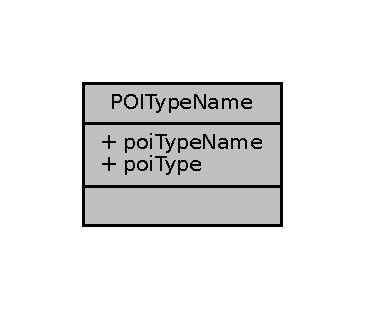
\includegraphics[width=175pt]{structPOITypeName__coll__graph}
\end{center}
\end{figure}
\subsection*{Public Attributes}
\begin{DoxyCompactItemize}
\item 
string \hyperlink{structPOITypeName_a2db157ca193d5d994f216f29377d24d1}{poi\+Type\+Name}
\item 
\hyperlink{classCPOI_a4b95e2e14055d2f9ca134e474dd4a19f}{C\+P\+O\+I\+::t\+\_\+poi} \hyperlink{structPOITypeName_a01d9d6fe156e851207e9c765bd4defaf}{poi\+Type}
\end{DoxyCompactItemize}


\subsection{Member Data Documentation}
\mbox{\Hypertarget{structPOITypeName_a01d9d6fe156e851207e9c765bd4defaf}\label{structPOITypeName_a01d9d6fe156e851207e9c765bd4defaf}} 
\index{P\+O\+I\+Type\+Name@{P\+O\+I\+Type\+Name}!poi\+Type@{poi\+Type}}
\index{poi\+Type@{poi\+Type}!P\+O\+I\+Type\+Name@{P\+O\+I\+Type\+Name}}
\subsubsection{\texorpdfstring{poi\+Type}{poiType}}
{\footnotesize\ttfamily \hyperlink{classCPOI_a4b95e2e14055d2f9ca134e474dd4a19f}{C\+P\+O\+I\+::t\+\_\+poi} P\+O\+I\+Type\+Name\+::poi\+Type}

\mbox{\Hypertarget{structPOITypeName_a2db157ca193d5d994f216f29377d24d1}\label{structPOITypeName_a2db157ca193d5d994f216f29377d24d1}} 
\index{P\+O\+I\+Type\+Name@{P\+O\+I\+Type\+Name}!poi\+Type\+Name@{poi\+Type\+Name}}
\index{poi\+Type\+Name@{poi\+Type\+Name}!P\+O\+I\+Type\+Name@{P\+O\+I\+Type\+Name}}
\subsubsection{\texorpdfstring{poi\+Type\+Name}{poiTypeName}}
{\footnotesize\ttfamily string P\+O\+I\+Type\+Name\+::poi\+Type\+Name}



The documentation for this struct was generated from the following file\+:\begin{DoxyCompactItemize}
\item 
\hyperlink{CPOI_8cpp}{C\+P\+O\+I.\+cpp}\end{DoxyCompactItemize}

\hypertarget{structyy__buffer__state}{}\section{yy\+\_\+buffer\+\_\+state Struct Reference}
\label{structyy__buffer__state}\index{yy\+\_\+buffer\+\_\+state@{yy\+\_\+buffer\+\_\+state}}


{\ttfamily \#include $<$lex.\+json.\+h$>$}



Collaboration diagram for yy\+\_\+buffer\+\_\+state\+:
\nopagebreak
\begin{figure}[H]
\begin{center}
\leavevmode
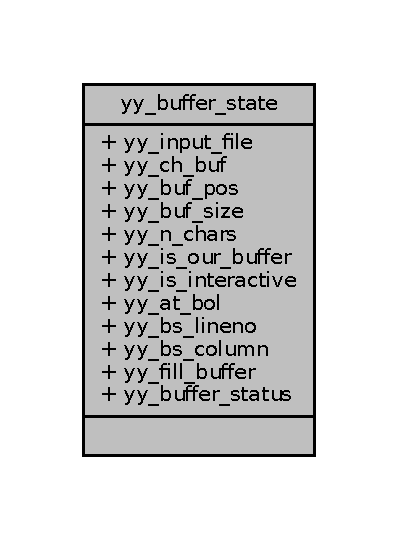
\includegraphics[width=191pt]{structyy__buffer__state__coll__graph}
\end{center}
\end{figure}
\subsection*{Public Attributes}
\begin{DoxyCompactItemize}
\item 
std\+::istream $\ast$ \hyperlink{structyy__buffer__state_a394bf1c9938ce57782dc313d97770123}{yy\+\_\+input\+\_\+file}
\item 
char $\ast$ \hyperlink{structyy__buffer__state_a0d25458e69eb22207fc633a1255d099d}{yy\+\_\+ch\+\_\+buf}
\item 
char $\ast$ \hyperlink{structyy__buffer__state_a8435c3f786bbb55d21d0174e4cfc22a0}{yy\+\_\+buf\+\_\+pos}
\item 
\hyperlink{lex_8json_8cc_ad557845057f187eec4be07e2717d2afa}{yy\+\_\+size\+\_\+t} \hyperlink{structyy__buffer__state_a48302f5f3477a9c78bbddf56d356ef54}{yy\+\_\+buf\+\_\+size}
\item 
\hyperlink{lex_8json_8cc_ad557845057f187eec4be07e2717d2afa}{yy\+\_\+size\+\_\+t} \hyperlink{structyy__buffer__state_afcc44872643f513e79b43c2b1f334a67}{yy\+\_\+n\+\_\+chars}
\item 
int \hyperlink{structyy__buffer__state_a80ce2431c70dc4f89ced487f18449465}{yy\+\_\+is\+\_\+our\+\_\+buffer}
\item 
int \hyperlink{structyy__buffer__state_abf5c70eea75581b58c0ee7bd31b14490}{yy\+\_\+is\+\_\+interactive}
\item 
int \hyperlink{structyy__buffer__state_a9d60c60af6e1a6f69de16871fd64f85f}{yy\+\_\+at\+\_\+bol}
\item 
int \hyperlink{structyy__buffer__state_a818e94bc9c766e683c60df1e9fd01199}{yy\+\_\+bs\+\_\+lineno}
\item 
int \hyperlink{structyy__buffer__state_a10c4fcd8be759e6bf11e6d3e8cdb0307}{yy\+\_\+bs\+\_\+column}
\item 
int \hyperlink{structyy__buffer__state_a63d2afbb1d79a3fc63df9e12626f827d}{yy\+\_\+fill\+\_\+buffer}
\item 
int \hyperlink{structyy__buffer__state_a70fd925d37a2f0454fbd0def675d106c}{yy\+\_\+buffer\+\_\+status}
\end{DoxyCompactItemize}


\subsection{Member Data Documentation}
\mbox{\Hypertarget{structyy__buffer__state_a9d60c60af6e1a6f69de16871fd64f85f}\label{structyy__buffer__state_a9d60c60af6e1a6f69de16871fd64f85f}} 
\index{yy\+\_\+buffer\+\_\+state@{yy\+\_\+buffer\+\_\+state}!yy\+\_\+at\+\_\+bol@{yy\+\_\+at\+\_\+bol}}
\index{yy\+\_\+at\+\_\+bol@{yy\+\_\+at\+\_\+bol}!yy\+\_\+buffer\+\_\+state@{yy\+\_\+buffer\+\_\+state}}
\subsubsection{\texorpdfstring{yy\+\_\+at\+\_\+bol}{yy\_at\_bol}}
{\footnotesize\ttfamily int yy\+\_\+buffer\+\_\+state\+::yy\+\_\+at\+\_\+bol}

\mbox{\Hypertarget{structyy__buffer__state_a10c4fcd8be759e6bf11e6d3e8cdb0307}\label{structyy__buffer__state_a10c4fcd8be759e6bf11e6d3e8cdb0307}} 
\index{yy\+\_\+buffer\+\_\+state@{yy\+\_\+buffer\+\_\+state}!yy\+\_\+bs\+\_\+column@{yy\+\_\+bs\+\_\+column}}
\index{yy\+\_\+bs\+\_\+column@{yy\+\_\+bs\+\_\+column}!yy\+\_\+buffer\+\_\+state@{yy\+\_\+buffer\+\_\+state}}
\subsubsection{\texorpdfstring{yy\+\_\+bs\+\_\+column}{yy\_bs\_column}}
{\footnotesize\ttfamily int yy\+\_\+buffer\+\_\+state\+::yy\+\_\+bs\+\_\+column}

The column count. \mbox{\Hypertarget{structyy__buffer__state_a818e94bc9c766e683c60df1e9fd01199}\label{structyy__buffer__state_a818e94bc9c766e683c60df1e9fd01199}} 
\index{yy\+\_\+buffer\+\_\+state@{yy\+\_\+buffer\+\_\+state}!yy\+\_\+bs\+\_\+lineno@{yy\+\_\+bs\+\_\+lineno}}
\index{yy\+\_\+bs\+\_\+lineno@{yy\+\_\+bs\+\_\+lineno}!yy\+\_\+buffer\+\_\+state@{yy\+\_\+buffer\+\_\+state}}
\subsubsection{\texorpdfstring{yy\+\_\+bs\+\_\+lineno}{yy\_bs\_lineno}}
{\footnotesize\ttfamily int yy\+\_\+buffer\+\_\+state\+::yy\+\_\+bs\+\_\+lineno}

The line count. \mbox{\Hypertarget{structyy__buffer__state_a8435c3f786bbb55d21d0174e4cfc22a0}\label{structyy__buffer__state_a8435c3f786bbb55d21d0174e4cfc22a0}} 
\index{yy\+\_\+buffer\+\_\+state@{yy\+\_\+buffer\+\_\+state}!yy\+\_\+buf\+\_\+pos@{yy\+\_\+buf\+\_\+pos}}
\index{yy\+\_\+buf\+\_\+pos@{yy\+\_\+buf\+\_\+pos}!yy\+\_\+buffer\+\_\+state@{yy\+\_\+buffer\+\_\+state}}
\subsubsection{\texorpdfstring{yy\+\_\+buf\+\_\+pos}{yy\_buf\_pos}}
{\footnotesize\ttfamily char $\ast$ yy\+\_\+buffer\+\_\+state\+::yy\+\_\+buf\+\_\+pos}

\mbox{\Hypertarget{structyy__buffer__state_a48302f5f3477a9c78bbddf56d356ef54}\label{structyy__buffer__state_a48302f5f3477a9c78bbddf56d356ef54}} 
\index{yy\+\_\+buffer\+\_\+state@{yy\+\_\+buffer\+\_\+state}!yy\+\_\+buf\+\_\+size@{yy\+\_\+buf\+\_\+size}}
\index{yy\+\_\+buf\+\_\+size@{yy\+\_\+buf\+\_\+size}!yy\+\_\+buffer\+\_\+state@{yy\+\_\+buffer\+\_\+state}}
\subsubsection{\texorpdfstring{yy\+\_\+buf\+\_\+size}{yy\_buf\_size}}
{\footnotesize\ttfamily \hyperlink{lex_8json_8cc_ad557845057f187eec4be07e2717d2afa}{yy\+\_\+size\+\_\+t} yy\+\_\+buffer\+\_\+state\+::yy\+\_\+buf\+\_\+size}

\mbox{\Hypertarget{structyy__buffer__state_a70fd925d37a2f0454fbd0def675d106c}\label{structyy__buffer__state_a70fd925d37a2f0454fbd0def675d106c}} 
\index{yy\+\_\+buffer\+\_\+state@{yy\+\_\+buffer\+\_\+state}!yy\+\_\+buffer\+\_\+status@{yy\+\_\+buffer\+\_\+status}}
\index{yy\+\_\+buffer\+\_\+status@{yy\+\_\+buffer\+\_\+status}!yy\+\_\+buffer\+\_\+state@{yy\+\_\+buffer\+\_\+state}}
\subsubsection{\texorpdfstring{yy\+\_\+buffer\+\_\+status}{yy\_buffer\_status}}
{\footnotesize\ttfamily int yy\+\_\+buffer\+\_\+state\+::yy\+\_\+buffer\+\_\+status}

\mbox{\Hypertarget{structyy__buffer__state_a0d25458e69eb22207fc633a1255d099d}\label{structyy__buffer__state_a0d25458e69eb22207fc633a1255d099d}} 
\index{yy\+\_\+buffer\+\_\+state@{yy\+\_\+buffer\+\_\+state}!yy\+\_\+ch\+\_\+buf@{yy\+\_\+ch\+\_\+buf}}
\index{yy\+\_\+ch\+\_\+buf@{yy\+\_\+ch\+\_\+buf}!yy\+\_\+buffer\+\_\+state@{yy\+\_\+buffer\+\_\+state}}
\subsubsection{\texorpdfstring{yy\+\_\+ch\+\_\+buf}{yy\_ch\_buf}}
{\footnotesize\ttfamily char $\ast$ yy\+\_\+buffer\+\_\+state\+::yy\+\_\+ch\+\_\+buf}

\mbox{\Hypertarget{structyy__buffer__state_a63d2afbb1d79a3fc63df9e12626f827d}\label{structyy__buffer__state_a63d2afbb1d79a3fc63df9e12626f827d}} 
\index{yy\+\_\+buffer\+\_\+state@{yy\+\_\+buffer\+\_\+state}!yy\+\_\+fill\+\_\+buffer@{yy\+\_\+fill\+\_\+buffer}}
\index{yy\+\_\+fill\+\_\+buffer@{yy\+\_\+fill\+\_\+buffer}!yy\+\_\+buffer\+\_\+state@{yy\+\_\+buffer\+\_\+state}}
\subsubsection{\texorpdfstring{yy\+\_\+fill\+\_\+buffer}{yy\_fill\_buffer}}
{\footnotesize\ttfamily int yy\+\_\+buffer\+\_\+state\+::yy\+\_\+fill\+\_\+buffer}

\mbox{\Hypertarget{structyy__buffer__state_a394bf1c9938ce57782dc313d97770123}\label{structyy__buffer__state_a394bf1c9938ce57782dc313d97770123}} 
\index{yy\+\_\+buffer\+\_\+state@{yy\+\_\+buffer\+\_\+state}!yy\+\_\+input\+\_\+file@{yy\+\_\+input\+\_\+file}}
\index{yy\+\_\+input\+\_\+file@{yy\+\_\+input\+\_\+file}!yy\+\_\+buffer\+\_\+state@{yy\+\_\+buffer\+\_\+state}}
\subsubsection{\texorpdfstring{yy\+\_\+input\+\_\+file}{yy\_input\_file}}
{\footnotesize\ttfamily std\+::istream $\ast$ yy\+\_\+buffer\+\_\+state\+::yy\+\_\+input\+\_\+file}

\mbox{\Hypertarget{structyy__buffer__state_abf5c70eea75581b58c0ee7bd31b14490}\label{structyy__buffer__state_abf5c70eea75581b58c0ee7bd31b14490}} 
\index{yy\+\_\+buffer\+\_\+state@{yy\+\_\+buffer\+\_\+state}!yy\+\_\+is\+\_\+interactive@{yy\+\_\+is\+\_\+interactive}}
\index{yy\+\_\+is\+\_\+interactive@{yy\+\_\+is\+\_\+interactive}!yy\+\_\+buffer\+\_\+state@{yy\+\_\+buffer\+\_\+state}}
\subsubsection{\texorpdfstring{yy\+\_\+is\+\_\+interactive}{yy\_is\_interactive}}
{\footnotesize\ttfamily int yy\+\_\+buffer\+\_\+state\+::yy\+\_\+is\+\_\+interactive}

\mbox{\Hypertarget{structyy__buffer__state_a80ce2431c70dc4f89ced487f18449465}\label{structyy__buffer__state_a80ce2431c70dc4f89ced487f18449465}} 
\index{yy\+\_\+buffer\+\_\+state@{yy\+\_\+buffer\+\_\+state}!yy\+\_\+is\+\_\+our\+\_\+buffer@{yy\+\_\+is\+\_\+our\+\_\+buffer}}
\index{yy\+\_\+is\+\_\+our\+\_\+buffer@{yy\+\_\+is\+\_\+our\+\_\+buffer}!yy\+\_\+buffer\+\_\+state@{yy\+\_\+buffer\+\_\+state}}
\subsubsection{\texorpdfstring{yy\+\_\+is\+\_\+our\+\_\+buffer}{yy\_is\_our\_buffer}}
{\footnotesize\ttfamily int yy\+\_\+buffer\+\_\+state\+::yy\+\_\+is\+\_\+our\+\_\+buffer}

\mbox{\Hypertarget{structyy__buffer__state_afcc44872643f513e79b43c2b1f334a67}\label{structyy__buffer__state_afcc44872643f513e79b43c2b1f334a67}} 
\index{yy\+\_\+buffer\+\_\+state@{yy\+\_\+buffer\+\_\+state}!yy\+\_\+n\+\_\+chars@{yy\+\_\+n\+\_\+chars}}
\index{yy\+\_\+n\+\_\+chars@{yy\+\_\+n\+\_\+chars}!yy\+\_\+buffer\+\_\+state@{yy\+\_\+buffer\+\_\+state}}
\subsubsection{\texorpdfstring{yy\+\_\+n\+\_\+chars}{yy\_n\_chars}}
{\footnotesize\ttfamily \hyperlink{lex_8json_8cc_ad557845057f187eec4be07e2717d2afa}{yy\+\_\+size\+\_\+t} yy\+\_\+buffer\+\_\+state\+::yy\+\_\+n\+\_\+chars}



The documentation for this struct was generated from the following files\+:\begin{DoxyCompactItemize}
\item 
\hyperlink{lex_8json_8cc}{lex.\+json.\+cc}\item 
\hyperlink{lex_8json_8h}{lex.\+json.\+h}\end{DoxyCompactItemize}

\hypertarget{structyy__trans__info}{}\section{yy\+\_\+trans\+\_\+info Struct Reference}
\label{structyy__trans__info}\index{yy\+\_\+trans\+\_\+info@{yy\+\_\+trans\+\_\+info}}


Collaboration diagram for yy\+\_\+trans\+\_\+info\+:
\nopagebreak
\begin{figure}[H]
\begin{center}
\leavevmode
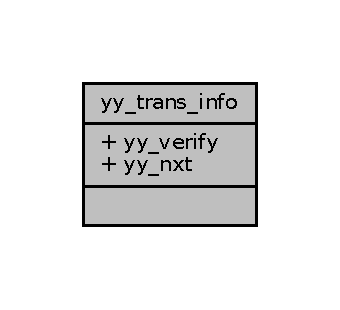
\includegraphics[width=163pt]{structyy__trans__info__coll__graph}
\end{center}
\end{figure}
\subsection*{Public Attributes}
\begin{DoxyCompactItemize}
\item 
\hyperlink{lex_8json_8cc_a838ce943cf44ef7769480714fc6c3ba9}{flex\+\_\+int32\+\_\+t} \hyperlink{structyy__trans__info_a5c9f61e770deef50bd4e697310342fe9}{yy\+\_\+verify}
\item 
\hyperlink{lex_8json_8cc_a838ce943cf44ef7769480714fc6c3ba9}{flex\+\_\+int32\+\_\+t} \hyperlink{structyy__trans__info_ae0715250c2bef261e596e77e0030f13e}{yy\+\_\+nxt}
\end{DoxyCompactItemize}


\subsection{Member Data Documentation}
\mbox{\Hypertarget{structyy__trans__info_ae0715250c2bef261e596e77e0030f13e}\label{structyy__trans__info_ae0715250c2bef261e596e77e0030f13e}} 
\index{yy\+\_\+trans\+\_\+info@{yy\+\_\+trans\+\_\+info}!yy\+\_\+nxt@{yy\+\_\+nxt}}
\index{yy\+\_\+nxt@{yy\+\_\+nxt}!yy\+\_\+trans\+\_\+info@{yy\+\_\+trans\+\_\+info}}
\subsubsection{\texorpdfstring{yy\+\_\+nxt}{yy\_nxt}}
{\footnotesize\ttfamily \hyperlink{lex_8json_8cc_a838ce943cf44ef7769480714fc6c3ba9}{flex\+\_\+int32\+\_\+t} yy\+\_\+trans\+\_\+info\+::yy\+\_\+nxt}

\mbox{\Hypertarget{structyy__trans__info_a5c9f61e770deef50bd4e697310342fe9}\label{structyy__trans__info_a5c9f61e770deef50bd4e697310342fe9}} 
\index{yy\+\_\+trans\+\_\+info@{yy\+\_\+trans\+\_\+info}!yy\+\_\+verify@{yy\+\_\+verify}}
\index{yy\+\_\+verify@{yy\+\_\+verify}!yy\+\_\+trans\+\_\+info@{yy\+\_\+trans\+\_\+info}}
\subsubsection{\texorpdfstring{yy\+\_\+verify}{yy\_verify}}
{\footnotesize\ttfamily \hyperlink{lex_8json_8cc_a838ce943cf44ef7769480714fc6c3ba9}{flex\+\_\+int32\+\_\+t} yy\+\_\+trans\+\_\+info\+::yy\+\_\+verify}



The documentation for this struct was generated from the following file\+:\begin{DoxyCompactItemize}
\item 
\hyperlink{lex_8json_8cc}{lex.\+json.\+cc}\end{DoxyCompactItemize}

\hypertarget{classyyFlexLexer}{}\section{yy\+Flex\+Lexer Class Reference}
\label{classyyFlexLexer}\index{yy\+Flex\+Lexer@{yy\+Flex\+Lexer}}


{\ttfamily \#include $<$Flex\+Lexer.\+h$>$}



Inheritance diagram for yy\+Flex\+Lexer\+:
\nopagebreak
\begin{figure}[H]
\begin{center}
\leavevmode
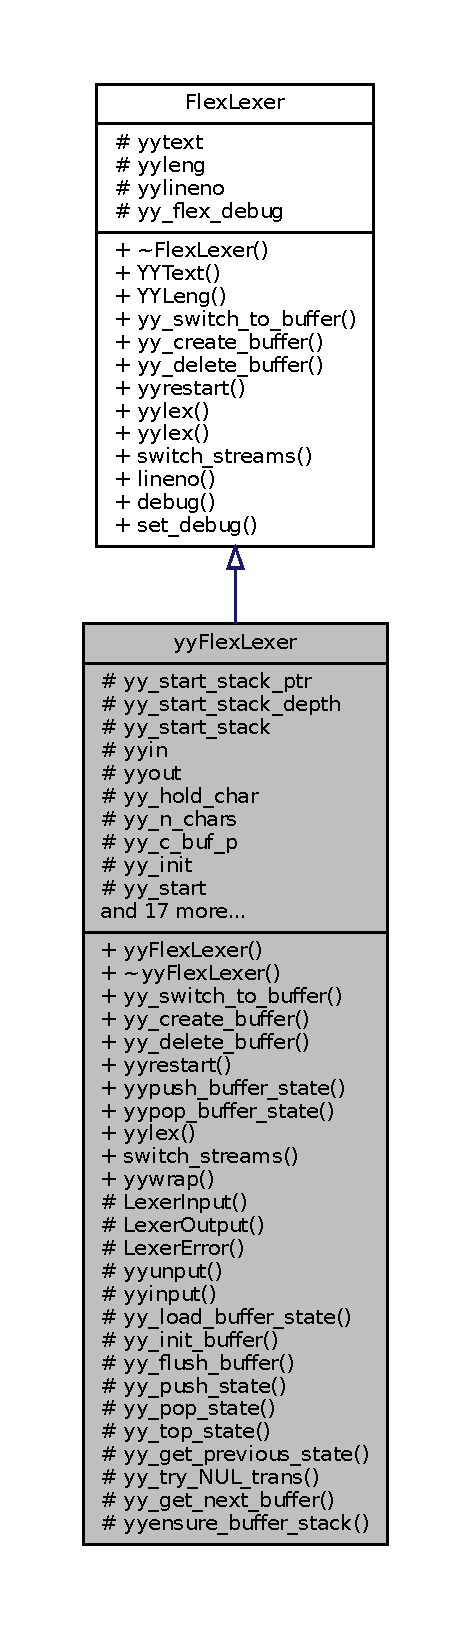
\includegraphics[height=550pt]{classyyFlexLexer__inherit__graph}
\end{center}
\end{figure}


Collaboration diagram for yy\+Flex\+Lexer\+:
\nopagebreak
\begin{figure}[H]
\begin{center}
\leavevmode
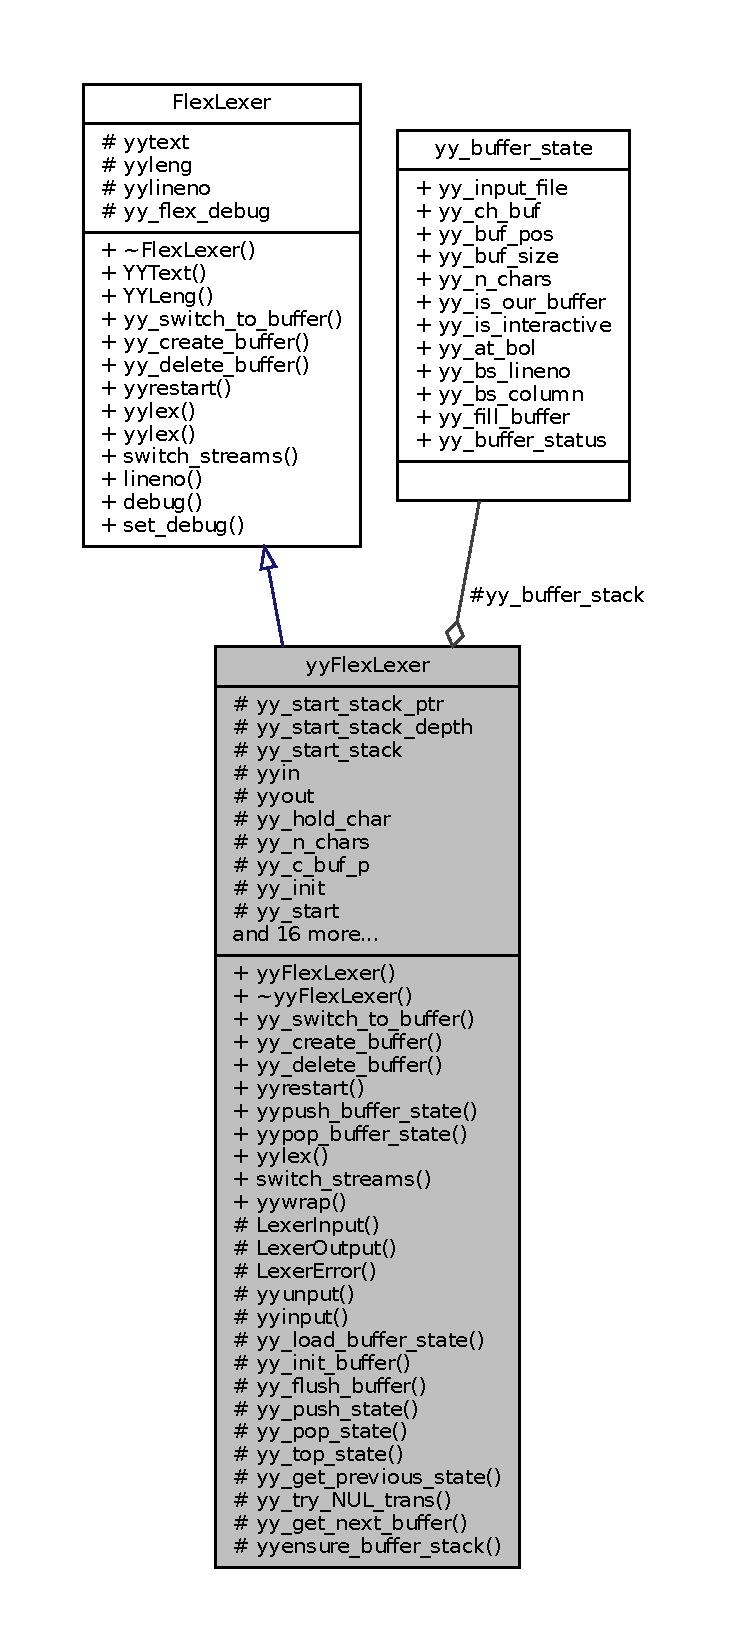
\includegraphics[height=550pt]{classyyFlexLexer__coll__graph}
\end{center}
\end{figure}
\subsection*{Public Member Functions}
\begin{DoxyCompactItemize}
\item 
\hyperlink{classyyFlexLexer_a327ec30fcb12fcdbff3a0b776ed40504}{yy\+Flex\+Lexer} (\hyperlink{FlexLexer_8h_ae50ff830f34b9e244163babb41a1552d}{F\+L\+E\+X\+\_\+\+S\+TD} istream $\ast$arg\+\_\+yyin=0, \hyperlink{FlexLexer_8h_ae50ff830f34b9e244163babb41a1552d}{F\+L\+E\+X\+\_\+\+S\+TD} ostream $\ast$arg\+\_\+yyout=0)
\item 
virtual \hyperlink{classyyFlexLexer_a7962c3ff1926bba84f4bdd831e99f85d}{$\sim$yy\+Flex\+Lexer} ()
\item 
void \hyperlink{classyyFlexLexer_ad1d304c93cf758e1ae4db98d9ca35ad0}{yy\+\_\+switch\+\_\+to\+\_\+buffer} (struct \hyperlink{structyy__buffer__state}{yy\+\_\+buffer\+\_\+state} $\ast$new\+\_\+buffer)
\item 
struct \hyperlink{structyy__buffer__state}{yy\+\_\+buffer\+\_\+state} $\ast$ \hyperlink{classyyFlexLexer_ac72d57010353577c918e72eba3d8972a}{yy\+\_\+create\+\_\+buffer} (\hyperlink{FlexLexer_8h_ae50ff830f34b9e244163babb41a1552d}{F\+L\+E\+X\+\_\+\+S\+TD} istream $\ast$s, int size)
\item 
void \hyperlink{classyyFlexLexer_a645a8ebb5b2b5b80707d053a0eb7a21a}{yy\+\_\+delete\+\_\+buffer} (struct \hyperlink{structyy__buffer__state}{yy\+\_\+buffer\+\_\+state} $\ast$b)
\item 
void \hyperlink{classyyFlexLexer_ab337dd3bd9504644164c0600d960b6e2}{yyrestart} (\hyperlink{FlexLexer_8h_ae50ff830f34b9e244163babb41a1552d}{F\+L\+E\+X\+\_\+\+S\+TD} istream $\ast$s)
\item 
void \hyperlink{classyyFlexLexer_ad1c28db628d822013851d46fddbab4b2}{yypush\+\_\+buffer\+\_\+state} (struct \hyperlink{structyy__buffer__state}{yy\+\_\+buffer\+\_\+state} $\ast$new\+\_\+buffer)
\item 
void \hyperlink{classyyFlexLexer_a40740ddffd5cbf7b8f09ab0a7ee4fb3f}{yypop\+\_\+buffer\+\_\+state} ()
\item 
virtual int \hyperlink{classyyFlexLexer_a49826cc55dd4c5e668d9391b80a57274}{yylex} ()
\item 
virtual void \hyperlink{classyyFlexLexer_ae88d47b620670ef7a924f4fe1e70774b}{switch\+\_\+streams} (\hyperlink{FlexLexer_8h_ae50ff830f34b9e244163babb41a1552d}{F\+L\+E\+X\+\_\+\+S\+TD} istream $\ast$new\+\_\+in, \hyperlink{FlexLexer_8h_ae50ff830f34b9e244163babb41a1552d}{F\+L\+E\+X\+\_\+\+S\+TD} ostream $\ast$new\+\_\+out=0)
\item 
virtual int \hyperlink{classyyFlexLexer_a9e46b16e6374b1b7ae696e2ba5fdc07c}{yywrap} ()
\end{DoxyCompactItemize}
\subsection*{Protected Member Functions}
\begin{DoxyCompactItemize}
\item 
virtual int \hyperlink{classyyFlexLexer_a285bb6cb3d9132ec16e2cbd3fb766ae9}{Lexer\+Input} (char $\ast$buf, int max\+\_\+size)
\item 
virtual void \hyperlink{classyyFlexLexer_ae037fa792625995f3f7b4dc65769d8f8}{Lexer\+Output} (const char $\ast$buf, int size)
\item 
virtual void \hyperlink{classyyFlexLexer_a8e3e041273a08400c0da07781f6682cf}{Lexer\+Error} (const char $\ast$msg)
\item 
void \hyperlink{classyyFlexLexer_a54064ce670d0caa1a45c5656d5e11538}{yyunput} (int c, char $\ast$buf\+\_\+ptr)
\item 
int \hyperlink{classyyFlexLexer_a4560699d55cb842ea01ca38e595afd95}{yyinput} ()
\item 
void \hyperlink{classyyFlexLexer_acc37b2da3bc88ae411e2009c8a534ee3}{yy\+\_\+load\+\_\+buffer\+\_\+state} ()
\item 
void \hyperlink{classyyFlexLexer_a4e12c1075d2e20c6de18c1220b0d90e2}{yy\+\_\+init\+\_\+buffer} (struct \hyperlink{structyy__buffer__state}{yy\+\_\+buffer\+\_\+state} $\ast$b, \hyperlink{FlexLexer_8h_ae50ff830f34b9e244163babb41a1552d}{F\+L\+E\+X\+\_\+\+S\+TD} istream $\ast$s)
\item 
void \hyperlink{classyyFlexLexer_ae2c2e8f3beb40d55311864d867493d68}{yy\+\_\+flush\+\_\+buffer} (struct \hyperlink{structyy__buffer__state}{yy\+\_\+buffer\+\_\+state} $\ast$b)
\item 
void \hyperlink{classyyFlexLexer_a6246bcfbf2bed9f3497d4f6398e11706}{yy\+\_\+push\+\_\+state} (int new\+\_\+state)
\item 
void \hyperlink{classyyFlexLexer_a58ea71e548fedec914d814a3e320efe9}{yy\+\_\+pop\+\_\+state} ()
\item 
int \hyperlink{classyyFlexLexer_aa1ae2fa3798a4d520bc846052207f562}{yy\+\_\+top\+\_\+state} ()
\item 
\hyperlink{FlexLexer_8h_a9ba7c416f135b0f0c1f4addded4616b5}{yy\+\_\+state\+\_\+type} \hyperlink{classyyFlexLexer_a8e2236ff4238b19413f3d19dc6f5a8dd}{yy\+\_\+get\+\_\+previous\+\_\+state} ()
\item 
\hyperlink{FlexLexer_8h_a9ba7c416f135b0f0c1f4addded4616b5}{yy\+\_\+state\+\_\+type} \hyperlink{classyyFlexLexer_ac58babd5c2cb9b7ba0b08cbc0898c89f}{yy\+\_\+try\+\_\+\+N\+U\+L\+\_\+trans} (\hyperlink{FlexLexer_8h_a9ba7c416f135b0f0c1f4addded4616b5}{yy\+\_\+state\+\_\+type} current\+\_\+state)
\item 
int \hyperlink{classyyFlexLexer_a3659121edfbb2d06999b22ca9255fb1a}{yy\+\_\+get\+\_\+next\+\_\+buffer} ()
\item 
void \hyperlink{classyyFlexLexer_a12af5c2b352914fabe55dfa8b1a77a15}{yyensure\+\_\+buffer\+\_\+stack} (void)
\end{DoxyCompactItemize}
\subsection*{Protected Attributes}
\begin{DoxyCompactItemize}
\item 
int \hyperlink{classyyFlexLexer_a45cf5f774631413c0d7aa820e8acb761}{yy\+\_\+start\+\_\+stack\+\_\+ptr}
\item 
int \hyperlink{classyyFlexLexer_a23f6dda98adbcbe13cfbfd1c74efc66f}{yy\+\_\+start\+\_\+stack\+\_\+depth}
\item 
int $\ast$ \hyperlink{classyyFlexLexer_abbb8bfcab69577e4d708e33c4627967d}{yy\+\_\+start\+\_\+stack}
\item 
\hyperlink{FlexLexer_8h_ae50ff830f34b9e244163babb41a1552d}{F\+L\+E\+X\+\_\+\+S\+TD} istream $\ast$ \hyperlink{classyyFlexLexer_a5be30a2c4ed9973f0ede10322ca9dbe8}{yyin}
\item 
\hyperlink{FlexLexer_8h_ae50ff830f34b9e244163babb41a1552d}{F\+L\+E\+X\+\_\+\+S\+TD} ostream $\ast$ \hyperlink{classyyFlexLexer_ac78543eed2c5f96cb6e4256450f0a923}{yyout}
\item 
char \hyperlink{classyyFlexLexer_a11b21266d7c772de839fe15c978e84be}{yy\+\_\+hold\+\_\+char}
\item 
int \hyperlink{classyyFlexLexer_ac2fa33e27e117953f53738b85d56353c}{yy\+\_\+n\+\_\+chars}
\item 
char $\ast$ \hyperlink{classyyFlexLexer_a117a76190eab99960a06ec667dee9abc}{yy\+\_\+c\+\_\+buf\+\_\+p}
\item 
int \hyperlink{classyyFlexLexer_a41cf7d4197a347a025cd10e042315bc4}{yy\+\_\+init}
\item 
int \hyperlink{classyyFlexLexer_afcad81a77535144e11e2a897eaa724b7}{yy\+\_\+start}
\item 
int \hyperlink{classyyFlexLexer_afdb4b21e0d512793a74d2eff444bffa9}{yy\+\_\+did\+\_\+buffer\+\_\+switch\+\_\+on\+\_\+eof}
\item 
size\+\_\+t \hyperlink{classyyFlexLexer_ad30ce09b0f06b749463bb1ddc8f74877}{yy\+\_\+buffer\+\_\+stack\+\_\+top}
\item 
size\+\_\+t \hyperlink{classyyFlexLexer_ad94e6d3987eb9dad09041a5cb006da7b}{yy\+\_\+buffer\+\_\+stack\+\_\+max}
\item 
struct \hyperlink{structyy__buffer__state}{yy\+\_\+buffer\+\_\+state} $\ast$$\ast$ \hyperlink{classyyFlexLexer_ae4914f003bda6f0dfc20e30703673bea}{yy\+\_\+buffer\+\_\+stack}
\item 
\hyperlink{FlexLexer_8h_a9ba7c416f135b0f0c1f4addded4616b5}{yy\+\_\+state\+\_\+type} \hyperlink{classyyFlexLexer_a7f55fb6c3dadf359d4085ecb88a39bc3}{yy\+\_\+last\+\_\+accepting\+\_\+state}
\item 
char $\ast$ \hyperlink{classyyFlexLexer_a488e654c851a95f0e18e00278d0f6f0b}{yy\+\_\+last\+\_\+accepting\+\_\+cpos}
\item 
\hyperlink{FlexLexer_8h_a9ba7c416f135b0f0c1f4addded4616b5}{yy\+\_\+state\+\_\+type} $\ast$ \hyperlink{classyyFlexLexer_aae59bd9cba37e88415d23335ba325c70}{yy\+\_\+state\+\_\+buf}
\item 
\hyperlink{FlexLexer_8h_a9ba7c416f135b0f0c1f4addded4616b5}{yy\+\_\+state\+\_\+type} $\ast$ \hyperlink{classyyFlexLexer_a7070807bda77c514273574e1a7e371d4}{yy\+\_\+state\+\_\+ptr}
\item 
char $\ast$ \hyperlink{classyyFlexLexer_a2c7312ae0d1942c35c4d9a807a498d5a}{yy\+\_\+full\+\_\+match}
\item 
int $\ast$ \hyperlink{classyyFlexLexer_aa58660405fbe6d717216f23d32adbd20}{yy\+\_\+full\+\_\+state}
\item 
int \hyperlink{classyyFlexLexer_a098331aae82780c3eb3ad9f63795f426}{yy\+\_\+full\+\_\+lp}
\item 
int \hyperlink{classyyFlexLexer_a871eaaa926a2a9f30bd32b74b66086de}{yy\+\_\+lp}
\item 
int \hyperlink{classyyFlexLexer_abd1ffa5da6e43ba3c793b47afed9a021}{yy\+\_\+looking\+\_\+for\+\_\+trail\+\_\+begin}
\item 
int \hyperlink{classyyFlexLexer_a4307cac1084ef13216ac81f053612328}{yy\+\_\+more\+\_\+flag}
\item 
int \hyperlink{classyyFlexLexer_a4e2974edc8f7f6f12e0bd804c8e71c59}{yy\+\_\+more\+\_\+len}
\item 
int \hyperlink{classyyFlexLexer_ae29ac547c7898e6b3ed19cda622e95e7}{yy\+\_\+more\+\_\+offset}
\item 
int \hyperlink{classyyFlexLexer_afcb935f8692299f97a78fb77b1e67ed0}{yy\+\_\+prev\+\_\+more\+\_\+offset}
\end{DoxyCompactItemize}


\subsection{Constructor \& Destructor Documentation}
\mbox{\Hypertarget{classyyFlexLexer_a327ec30fcb12fcdbff3a0b776ed40504}\label{classyyFlexLexer_a327ec30fcb12fcdbff3a0b776ed40504}} 
\index{yy\+Flex\+Lexer@{yy\+Flex\+Lexer}!yy\+Flex\+Lexer@{yy\+Flex\+Lexer}}
\index{yy\+Flex\+Lexer@{yy\+Flex\+Lexer}!yy\+Flex\+Lexer@{yy\+Flex\+Lexer}}
\subsubsection{\texorpdfstring{yy\+Flex\+Lexer()}{yyFlexLexer()}}
{\footnotesize\ttfamily yy\+Flex\+Lexer\+::yy\+Flex\+Lexer (\begin{DoxyParamCaption}\item[{\hyperlink{FlexLexer_8h_ae50ff830f34b9e244163babb41a1552d}{F\+L\+E\+X\+\_\+\+S\+TD} istream $\ast$}]{arg\+\_\+yyin = {\ttfamily 0},  }\item[{\hyperlink{FlexLexer_8h_ae50ff830f34b9e244163babb41a1552d}{F\+L\+E\+X\+\_\+\+S\+TD} ostream $\ast$}]{arg\+\_\+yyout = {\ttfamily 0} }\end{DoxyParamCaption})}

\mbox{\Hypertarget{classyyFlexLexer_a7962c3ff1926bba84f4bdd831e99f85d}\label{classyyFlexLexer_a7962c3ff1926bba84f4bdd831e99f85d}} 
\index{yy\+Flex\+Lexer@{yy\+Flex\+Lexer}!````~yy\+Flex\+Lexer@{$\sim$yy\+Flex\+Lexer}}
\index{````~yy\+Flex\+Lexer@{$\sim$yy\+Flex\+Lexer}!yy\+Flex\+Lexer@{yy\+Flex\+Lexer}}
\subsubsection{\texorpdfstring{$\sim$yy\+Flex\+Lexer()}{~yyFlexLexer()}}
{\footnotesize\ttfamily yy\+Flex\+Lexer\+::$\sim$yy\+Flex\+Lexer (\begin{DoxyParamCaption}{ }\end{DoxyParamCaption})\hspace{0.3cm}{\ttfamily [virtual]}}



\subsection{Member Function Documentation}
\mbox{\Hypertarget{classyyFlexLexer_a8e3e041273a08400c0da07781f6682cf}\label{classyyFlexLexer_a8e3e041273a08400c0da07781f6682cf}} 
\index{yy\+Flex\+Lexer@{yy\+Flex\+Lexer}!Lexer\+Error@{Lexer\+Error}}
\index{Lexer\+Error@{Lexer\+Error}!yy\+Flex\+Lexer@{yy\+Flex\+Lexer}}
\subsubsection{\texorpdfstring{Lexer\+Error()}{LexerError()}}
{\footnotesize\ttfamily void yy\+Flex\+Lexer\+::\+Lexer\+Error (\begin{DoxyParamCaption}\item[{const char $\ast$}]{msg }\end{DoxyParamCaption})\hspace{0.3cm}{\ttfamily [protected]}, {\ttfamily [virtual]}}

\mbox{\Hypertarget{classyyFlexLexer_a285bb6cb3d9132ec16e2cbd3fb766ae9}\label{classyyFlexLexer_a285bb6cb3d9132ec16e2cbd3fb766ae9}} 
\index{yy\+Flex\+Lexer@{yy\+Flex\+Lexer}!Lexer\+Input@{Lexer\+Input}}
\index{Lexer\+Input@{Lexer\+Input}!yy\+Flex\+Lexer@{yy\+Flex\+Lexer}}
\subsubsection{\texorpdfstring{Lexer\+Input()}{LexerInput()}}
{\footnotesize\ttfamily int yy\+Flex\+Lexer\+::\+Lexer\+Input (\begin{DoxyParamCaption}\item[{char $\ast$}]{buf,  }\item[{int}]{max\+\_\+size }\end{DoxyParamCaption})\hspace{0.3cm}{\ttfamily [protected]}, {\ttfamily [virtual]}}

\mbox{\Hypertarget{classyyFlexLexer_ae037fa792625995f3f7b4dc65769d8f8}\label{classyyFlexLexer_ae037fa792625995f3f7b4dc65769d8f8}} 
\index{yy\+Flex\+Lexer@{yy\+Flex\+Lexer}!Lexer\+Output@{Lexer\+Output}}
\index{Lexer\+Output@{Lexer\+Output}!yy\+Flex\+Lexer@{yy\+Flex\+Lexer}}
\subsubsection{\texorpdfstring{Lexer\+Output()}{LexerOutput()}}
{\footnotesize\ttfamily void yy\+Flex\+Lexer\+::\+Lexer\+Output (\begin{DoxyParamCaption}\item[{const char $\ast$}]{buf,  }\item[{int}]{size }\end{DoxyParamCaption})\hspace{0.3cm}{\ttfamily [protected]}, {\ttfamily [virtual]}}

\mbox{\Hypertarget{classyyFlexLexer_ae88d47b620670ef7a924f4fe1e70774b}\label{classyyFlexLexer_ae88d47b620670ef7a924f4fe1e70774b}} 
\index{yy\+Flex\+Lexer@{yy\+Flex\+Lexer}!switch\+\_\+streams@{switch\+\_\+streams}}
\index{switch\+\_\+streams@{switch\+\_\+streams}!yy\+Flex\+Lexer@{yy\+Flex\+Lexer}}
\subsubsection{\texorpdfstring{switch\+\_\+streams()}{switch\_streams()}}
{\footnotesize\ttfamily void yy\+Flex\+Lexer\+::switch\+\_\+streams (\begin{DoxyParamCaption}\item[{\hyperlink{FlexLexer_8h_ae50ff830f34b9e244163babb41a1552d}{F\+L\+E\+X\+\_\+\+S\+TD} istream $\ast$}]{new\+\_\+in,  }\item[{\hyperlink{FlexLexer_8h_ae50ff830f34b9e244163babb41a1552d}{F\+L\+E\+X\+\_\+\+S\+TD} ostream $\ast$}]{new\+\_\+out = {\ttfamily 0} }\end{DoxyParamCaption})\hspace{0.3cm}{\ttfamily [virtual]}}



Implements \hyperlink{classFlexLexer_a09dd0826a8540365a74c2167795bbc61}{Flex\+Lexer}.

\mbox{\Hypertarget{classyyFlexLexer_ac72d57010353577c918e72eba3d8972a}\label{classyyFlexLexer_ac72d57010353577c918e72eba3d8972a}} 
\index{yy\+Flex\+Lexer@{yy\+Flex\+Lexer}!yy\+\_\+create\+\_\+buffer@{yy\+\_\+create\+\_\+buffer}}
\index{yy\+\_\+create\+\_\+buffer@{yy\+\_\+create\+\_\+buffer}!yy\+Flex\+Lexer@{yy\+Flex\+Lexer}}
\subsubsection{\texorpdfstring{yy\+\_\+create\+\_\+buffer()}{yy\_create\_buffer()}}
{\footnotesize\ttfamily \hyperlink{lex_8json_8cc_a4e5bd2d129903df83f3d13effaf8f3e4}{Y\+Y\+\_\+\+B\+U\+F\+F\+E\+R\+\_\+\+S\+T\+A\+TE} yy\+Flex\+Lexer\+::yy\+\_\+create\+\_\+buffer (\begin{DoxyParamCaption}\item[{\hyperlink{FlexLexer_8h_ae50ff830f34b9e244163babb41a1552d}{F\+L\+E\+X\+\_\+\+S\+TD} istream $\ast$}]{s,  }\item[{int}]{size }\end{DoxyParamCaption})\hspace{0.3cm}{\ttfamily [virtual]}}

Allocate and initialize an input buffer state. 
\begin{DoxyParams}{Parameters}
{\em file} & A readable stream. \\
\hline
{\em size} & The character buffer size in bytes. When in doubt, use {\ttfamily Y\+Y\+\_\+\+B\+U\+F\+\_\+\+S\+I\+ZE}.\\
\hline
\end{DoxyParams}
\begin{DoxyReturn}{Returns}
the allocated buffer state. 
\end{DoxyReturn}


Implements \hyperlink{classFlexLexer_a9e0d5e33726e0270b241a730a3028990}{Flex\+Lexer}.

\mbox{\Hypertarget{classyyFlexLexer_a645a8ebb5b2b5b80707d053a0eb7a21a}\label{classyyFlexLexer_a645a8ebb5b2b5b80707d053a0eb7a21a}} 
\index{yy\+Flex\+Lexer@{yy\+Flex\+Lexer}!yy\+\_\+delete\+\_\+buffer@{yy\+\_\+delete\+\_\+buffer}}
\index{yy\+\_\+delete\+\_\+buffer@{yy\+\_\+delete\+\_\+buffer}!yy\+Flex\+Lexer@{yy\+Flex\+Lexer}}
\subsubsection{\texorpdfstring{yy\+\_\+delete\+\_\+buffer()}{yy\_delete\_buffer()}}
{\footnotesize\ttfamily void yy\+Flex\+Lexer\+::yy\+\_\+delete\+\_\+buffer (\begin{DoxyParamCaption}\item[{struct \hyperlink{structyy__buffer__state}{yy\+\_\+buffer\+\_\+state} $\ast$}]{b }\end{DoxyParamCaption})\hspace{0.3cm}{\ttfamily [virtual]}}

Destroy the buffer. 
\begin{DoxyParams}{Parameters}
{\em b} & a buffer created with \hyperlink{classyyFlexLexer_ac72d57010353577c918e72eba3d8972a}{yy\+\_\+create\+\_\+buffer()} \\
\hline
\end{DoxyParams}


Implements \hyperlink{classFlexLexer_a6c59180ab84ba98af3704ba2cb018230}{Flex\+Lexer}.

\mbox{\Hypertarget{classyyFlexLexer_ae2c2e8f3beb40d55311864d867493d68}\label{classyyFlexLexer_ae2c2e8f3beb40d55311864d867493d68}} 
\index{yy\+Flex\+Lexer@{yy\+Flex\+Lexer}!yy\+\_\+flush\+\_\+buffer@{yy\+\_\+flush\+\_\+buffer}}
\index{yy\+\_\+flush\+\_\+buffer@{yy\+\_\+flush\+\_\+buffer}!yy\+Flex\+Lexer@{yy\+Flex\+Lexer}}
\subsubsection{\texorpdfstring{yy\+\_\+flush\+\_\+buffer()}{yy\_flush\_buffer()}}
{\footnotesize\ttfamily void yy\+Flex\+Lexer\+::yy\+\_\+flush\+\_\+buffer (\begin{DoxyParamCaption}\item[{struct \hyperlink{structyy__buffer__state}{yy\+\_\+buffer\+\_\+state} $\ast$}]{b }\end{DoxyParamCaption})\hspace{0.3cm}{\ttfamily [protected]}}

Discard all buffered characters. On the next scan, Y\+Y\+\_\+\+I\+N\+P\+UT will be called. 
\begin{DoxyParams}{Parameters}
{\em b} & the buffer state to be flushed, usually {\ttfamily Y\+Y\+\_\+\+C\+U\+R\+R\+E\+N\+T\+\_\+\+B\+U\+F\+F\+ER}. \\
\hline
\end{DoxyParams}
\mbox{\Hypertarget{classyyFlexLexer_a3659121edfbb2d06999b22ca9255fb1a}\label{classyyFlexLexer_a3659121edfbb2d06999b22ca9255fb1a}} 
\index{yy\+Flex\+Lexer@{yy\+Flex\+Lexer}!yy\+\_\+get\+\_\+next\+\_\+buffer@{yy\+\_\+get\+\_\+next\+\_\+buffer}}
\index{yy\+\_\+get\+\_\+next\+\_\+buffer@{yy\+\_\+get\+\_\+next\+\_\+buffer}!yy\+Flex\+Lexer@{yy\+Flex\+Lexer}}
\subsubsection{\texorpdfstring{yy\+\_\+get\+\_\+next\+\_\+buffer()}{yy\_get\_next\_buffer()}}
{\footnotesize\ttfamily int yy\+Flex\+Lexer\+::yy\+\_\+get\+\_\+next\+\_\+buffer (\begin{DoxyParamCaption}{ }\end{DoxyParamCaption})\hspace{0.3cm}{\ttfamily [protected]}}

\mbox{\Hypertarget{classyyFlexLexer_a8e2236ff4238b19413f3d19dc6f5a8dd}\label{classyyFlexLexer_a8e2236ff4238b19413f3d19dc6f5a8dd}} 
\index{yy\+Flex\+Lexer@{yy\+Flex\+Lexer}!yy\+\_\+get\+\_\+previous\+\_\+state@{yy\+\_\+get\+\_\+previous\+\_\+state}}
\index{yy\+\_\+get\+\_\+previous\+\_\+state@{yy\+\_\+get\+\_\+previous\+\_\+state}!yy\+Flex\+Lexer@{yy\+Flex\+Lexer}}
\subsubsection{\texorpdfstring{yy\+\_\+get\+\_\+previous\+\_\+state()}{yy\_get\_previous\_state()}}
{\footnotesize\ttfamily \hyperlink{FlexLexer_8h_a9ba7c416f135b0f0c1f4addded4616b5}{yy\+\_\+state\+\_\+type} yy\+Flex\+Lexer\+::yy\+\_\+get\+\_\+previous\+\_\+state (\begin{DoxyParamCaption}{ }\end{DoxyParamCaption})\hspace{0.3cm}{\ttfamily [protected]}}

\mbox{\Hypertarget{classyyFlexLexer_a4e12c1075d2e20c6de18c1220b0d90e2}\label{classyyFlexLexer_a4e12c1075d2e20c6de18c1220b0d90e2}} 
\index{yy\+Flex\+Lexer@{yy\+Flex\+Lexer}!yy\+\_\+init\+\_\+buffer@{yy\+\_\+init\+\_\+buffer}}
\index{yy\+\_\+init\+\_\+buffer@{yy\+\_\+init\+\_\+buffer}!yy\+Flex\+Lexer@{yy\+Flex\+Lexer}}
\subsubsection{\texorpdfstring{yy\+\_\+init\+\_\+buffer()}{yy\_init\_buffer()}}
{\footnotesize\ttfamily void yy\+Flex\+Lexer\+::yy\+\_\+init\+\_\+buffer (\begin{DoxyParamCaption}\item[{struct \hyperlink{structyy__buffer__state}{yy\+\_\+buffer\+\_\+state} $\ast$}]{b,  }\item[{\hyperlink{FlexLexer_8h_ae50ff830f34b9e244163babb41a1552d}{F\+L\+E\+X\+\_\+\+S\+TD} istream $\ast$}]{s }\end{DoxyParamCaption})\hspace{0.3cm}{\ttfamily [protected]}}

\mbox{\Hypertarget{classyyFlexLexer_acc37b2da3bc88ae411e2009c8a534ee3}\label{classyyFlexLexer_acc37b2da3bc88ae411e2009c8a534ee3}} 
\index{yy\+Flex\+Lexer@{yy\+Flex\+Lexer}!yy\+\_\+load\+\_\+buffer\+\_\+state@{yy\+\_\+load\+\_\+buffer\+\_\+state}}
\index{yy\+\_\+load\+\_\+buffer\+\_\+state@{yy\+\_\+load\+\_\+buffer\+\_\+state}!yy\+Flex\+Lexer@{yy\+Flex\+Lexer}}
\subsubsection{\texorpdfstring{yy\+\_\+load\+\_\+buffer\+\_\+state()}{yy\_load\_buffer\_state()}}
{\footnotesize\ttfamily void yy\+Flex\+Lexer\+::yy\+\_\+load\+\_\+buffer\+\_\+state (\begin{DoxyParamCaption}{ }\end{DoxyParamCaption})\hspace{0.3cm}{\ttfamily [protected]}}

\mbox{\Hypertarget{classyyFlexLexer_a58ea71e548fedec914d814a3e320efe9}\label{classyyFlexLexer_a58ea71e548fedec914d814a3e320efe9}} 
\index{yy\+Flex\+Lexer@{yy\+Flex\+Lexer}!yy\+\_\+pop\+\_\+state@{yy\+\_\+pop\+\_\+state}}
\index{yy\+\_\+pop\+\_\+state@{yy\+\_\+pop\+\_\+state}!yy\+Flex\+Lexer@{yy\+Flex\+Lexer}}
\subsubsection{\texorpdfstring{yy\+\_\+pop\+\_\+state()}{yy\_pop\_state()}}
{\footnotesize\ttfamily void yy\+Flex\+Lexer\+::yy\+\_\+pop\+\_\+state (\begin{DoxyParamCaption}{ }\end{DoxyParamCaption})\hspace{0.3cm}{\ttfamily [protected]}}

\mbox{\Hypertarget{classyyFlexLexer_a6246bcfbf2bed9f3497d4f6398e11706}\label{classyyFlexLexer_a6246bcfbf2bed9f3497d4f6398e11706}} 
\index{yy\+Flex\+Lexer@{yy\+Flex\+Lexer}!yy\+\_\+push\+\_\+state@{yy\+\_\+push\+\_\+state}}
\index{yy\+\_\+push\+\_\+state@{yy\+\_\+push\+\_\+state}!yy\+Flex\+Lexer@{yy\+Flex\+Lexer}}
\subsubsection{\texorpdfstring{yy\+\_\+push\+\_\+state()}{yy\_push\_state()}}
{\footnotesize\ttfamily void yy\+Flex\+Lexer\+::yy\+\_\+push\+\_\+state (\begin{DoxyParamCaption}\item[{int}]{new\+\_\+state }\end{DoxyParamCaption})\hspace{0.3cm}{\ttfamily [protected]}}

\mbox{\Hypertarget{classyyFlexLexer_ad1d304c93cf758e1ae4db98d9ca35ad0}\label{classyyFlexLexer_ad1d304c93cf758e1ae4db98d9ca35ad0}} 
\index{yy\+Flex\+Lexer@{yy\+Flex\+Lexer}!yy\+\_\+switch\+\_\+to\+\_\+buffer@{yy\+\_\+switch\+\_\+to\+\_\+buffer}}
\index{yy\+\_\+switch\+\_\+to\+\_\+buffer@{yy\+\_\+switch\+\_\+to\+\_\+buffer}!yy\+Flex\+Lexer@{yy\+Flex\+Lexer}}
\subsubsection{\texorpdfstring{yy\+\_\+switch\+\_\+to\+\_\+buffer()}{yy\_switch\_to\_buffer()}}
{\footnotesize\ttfamily void yy\+Flex\+Lexer\+::yy\+\_\+switch\+\_\+to\+\_\+buffer (\begin{DoxyParamCaption}\item[{struct \hyperlink{structyy__buffer__state}{yy\+\_\+buffer\+\_\+state} $\ast$}]{new\+\_\+buffer }\end{DoxyParamCaption})\hspace{0.3cm}{\ttfamily [virtual]}}

Switch to a different input buffer. 
\begin{DoxyParams}{Parameters}
{\em new\+\_\+buffer} & The new input buffer. \\
\hline
\end{DoxyParams}


Implements \hyperlink{classFlexLexer_a3fa4649c1866a483fc391923ca90ca1d}{Flex\+Lexer}.

\mbox{\Hypertarget{classyyFlexLexer_aa1ae2fa3798a4d520bc846052207f562}\label{classyyFlexLexer_aa1ae2fa3798a4d520bc846052207f562}} 
\index{yy\+Flex\+Lexer@{yy\+Flex\+Lexer}!yy\+\_\+top\+\_\+state@{yy\+\_\+top\+\_\+state}}
\index{yy\+\_\+top\+\_\+state@{yy\+\_\+top\+\_\+state}!yy\+Flex\+Lexer@{yy\+Flex\+Lexer}}
\subsubsection{\texorpdfstring{yy\+\_\+top\+\_\+state()}{yy\_top\_state()}}
{\footnotesize\ttfamily int yy\+Flex\+Lexer\+::yy\+\_\+top\+\_\+state (\begin{DoxyParamCaption}{ }\end{DoxyParamCaption})\hspace{0.3cm}{\ttfamily [protected]}}

\mbox{\Hypertarget{classyyFlexLexer_ac58babd5c2cb9b7ba0b08cbc0898c89f}\label{classyyFlexLexer_ac58babd5c2cb9b7ba0b08cbc0898c89f}} 
\index{yy\+Flex\+Lexer@{yy\+Flex\+Lexer}!yy\+\_\+try\+\_\+\+N\+U\+L\+\_\+trans@{yy\+\_\+try\+\_\+\+N\+U\+L\+\_\+trans}}
\index{yy\+\_\+try\+\_\+\+N\+U\+L\+\_\+trans@{yy\+\_\+try\+\_\+\+N\+U\+L\+\_\+trans}!yy\+Flex\+Lexer@{yy\+Flex\+Lexer}}
\subsubsection{\texorpdfstring{yy\+\_\+try\+\_\+\+N\+U\+L\+\_\+trans()}{yy\_try\_NUL\_trans()}}
{\footnotesize\ttfamily \hyperlink{FlexLexer_8h_a9ba7c416f135b0f0c1f4addded4616b5}{yy\+\_\+state\+\_\+type} yy\+Flex\+Lexer\+::yy\+\_\+try\+\_\+\+N\+U\+L\+\_\+trans (\begin{DoxyParamCaption}\item[{\hyperlink{FlexLexer_8h_a9ba7c416f135b0f0c1f4addded4616b5}{yy\+\_\+state\+\_\+type}}]{current\+\_\+state }\end{DoxyParamCaption})\hspace{0.3cm}{\ttfamily [protected]}}

\mbox{\Hypertarget{classyyFlexLexer_a12af5c2b352914fabe55dfa8b1a77a15}\label{classyyFlexLexer_a12af5c2b352914fabe55dfa8b1a77a15}} 
\index{yy\+Flex\+Lexer@{yy\+Flex\+Lexer}!yyensure\+\_\+buffer\+\_\+stack@{yyensure\+\_\+buffer\+\_\+stack}}
\index{yyensure\+\_\+buffer\+\_\+stack@{yyensure\+\_\+buffer\+\_\+stack}!yy\+Flex\+Lexer@{yy\+Flex\+Lexer}}
\subsubsection{\texorpdfstring{yyensure\+\_\+buffer\+\_\+stack()}{yyensure\_buffer\_stack()}}
{\footnotesize\ttfamily void yy\+Flex\+Lexer\+::yyensure\+\_\+buffer\+\_\+stack (\begin{DoxyParamCaption}\item[{void}]{ }\end{DoxyParamCaption})\hspace{0.3cm}{\ttfamily [protected]}}

\mbox{\Hypertarget{classyyFlexLexer_a4560699d55cb842ea01ca38e595afd95}\label{classyyFlexLexer_a4560699d55cb842ea01ca38e595afd95}} 
\index{yy\+Flex\+Lexer@{yy\+Flex\+Lexer}!yyinput@{yyinput}}
\index{yyinput@{yyinput}!yy\+Flex\+Lexer@{yy\+Flex\+Lexer}}
\subsubsection{\texorpdfstring{yyinput()}{yyinput()}}
{\footnotesize\ttfamily int yy\+Flex\+Lexer\+::yyinput (\begin{DoxyParamCaption}{ }\end{DoxyParamCaption})\hspace{0.3cm}{\ttfamily [protected]}}

\mbox{\Hypertarget{classyyFlexLexer_a49826cc55dd4c5e668d9391b80a57274}\label{classyyFlexLexer_a49826cc55dd4c5e668d9391b80a57274}} 
\index{yy\+Flex\+Lexer@{yy\+Flex\+Lexer}!yylex@{yylex}}
\index{yylex@{yylex}!yy\+Flex\+Lexer@{yy\+Flex\+Lexer}}
\subsubsection{\texorpdfstring{yylex()}{yylex()}}
{\footnotesize\ttfamily int yy\+Flex\+Lexer\+::yylex (\begin{DoxyParamCaption}{ }\end{DoxyParamCaption})\hspace{0.3cm}{\ttfamily [virtual]}}



Implements \hyperlink{classFlexLexer_a1b1f93d24f5a97f50eb1747fac568ccb}{Flex\+Lexer}.

\mbox{\Hypertarget{classyyFlexLexer_a40740ddffd5cbf7b8f09ab0a7ee4fb3f}\label{classyyFlexLexer_a40740ddffd5cbf7b8f09ab0a7ee4fb3f}} 
\index{yy\+Flex\+Lexer@{yy\+Flex\+Lexer}!yypop\+\_\+buffer\+\_\+state@{yypop\+\_\+buffer\+\_\+state}}
\index{yypop\+\_\+buffer\+\_\+state@{yypop\+\_\+buffer\+\_\+state}!yy\+Flex\+Lexer@{yy\+Flex\+Lexer}}
\subsubsection{\texorpdfstring{yypop\+\_\+buffer\+\_\+state()}{yypop\_buffer\_state()}}
{\footnotesize\ttfamily void yy\+Flex\+Lexer\+::yypop\+\_\+buffer\+\_\+state (\begin{DoxyParamCaption}\item[{void}]{ }\end{DoxyParamCaption})}

Removes and deletes the top of the stack, if present. The next element becomes the new top. \mbox{\Hypertarget{classyyFlexLexer_ad1c28db628d822013851d46fddbab4b2}\label{classyyFlexLexer_ad1c28db628d822013851d46fddbab4b2}} 
\index{yy\+Flex\+Lexer@{yy\+Flex\+Lexer}!yypush\+\_\+buffer\+\_\+state@{yypush\+\_\+buffer\+\_\+state}}
\index{yypush\+\_\+buffer\+\_\+state@{yypush\+\_\+buffer\+\_\+state}!yy\+Flex\+Lexer@{yy\+Flex\+Lexer}}
\subsubsection{\texorpdfstring{yypush\+\_\+buffer\+\_\+state()}{yypush\_buffer\_state()}}
{\footnotesize\ttfamily void yy\+Flex\+Lexer\+::yypush\+\_\+buffer\+\_\+state (\begin{DoxyParamCaption}\item[{struct \hyperlink{structyy__buffer__state}{yy\+\_\+buffer\+\_\+state} $\ast$}]{new\+\_\+buffer }\end{DoxyParamCaption})}

Pushes the new state onto the stack. The new state becomes the current state. This function will allocate the stack if necessary. 
\begin{DoxyParams}{Parameters}
{\em new\+\_\+buffer} & The new state. \\
\hline
\end{DoxyParams}
\mbox{\Hypertarget{classyyFlexLexer_ab337dd3bd9504644164c0600d960b6e2}\label{classyyFlexLexer_ab337dd3bd9504644164c0600d960b6e2}} 
\index{yy\+Flex\+Lexer@{yy\+Flex\+Lexer}!yyrestart@{yyrestart}}
\index{yyrestart@{yyrestart}!yy\+Flex\+Lexer@{yy\+Flex\+Lexer}}
\subsubsection{\texorpdfstring{yyrestart()}{yyrestart()}}
{\footnotesize\ttfamily void yy\+Flex\+Lexer\+::yyrestart (\begin{DoxyParamCaption}\item[{\hyperlink{FlexLexer_8h_ae50ff830f34b9e244163babb41a1552d}{F\+L\+E\+X\+\_\+\+S\+TD} istream $\ast$}]{s }\end{DoxyParamCaption})\hspace{0.3cm}{\ttfamily [virtual]}}

Immediately switch to a different input stream. 
\begin{DoxyParams}{Parameters}
{\em input\+\_\+file} & A readable stream.\\
\hline
\end{DoxyParams}
\begin{DoxyNote}{Note}
This function does not reset the start condition to {\ttfamily I\+N\+I\+T\+I\+AL} . 
\end{DoxyNote}


Implements \hyperlink{classFlexLexer_a15aea8e169874756674e4f79553e68ed}{Flex\+Lexer}.

\mbox{\Hypertarget{classyyFlexLexer_a54064ce670d0caa1a45c5656d5e11538}\label{classyyFlexLexer_a54064ce670d0caa1a45c5656d5e11538}} 
\index{yy\+Flex\+Lexer@{yy\+Flex\+Lexer}!yyunput@{yyunput}}
\index{yyunput@{yyunput}!yy\+Flex\+Lexer@{yy\+Flex\+Lexer}}
\subsubsection{\texorpdfstring{yyunput()}{yyunput()}}
{\footnotesize\ttfamily void yy\+Flex\+Lexer\+::yyunput (\begin{DoxyParamCaption}\item[{int}]{c,  }\item[{char $\ast$}]{buf\+\_\+ptr }\end{DoxyParamCaption})\hspace{0.3cm}{\ttfamily [protected]}}

\mbox{\Hypertarget{classyyFlexLexer_a9e46b16e6374b1b7ae696e2ba5fdc07c}\label{classyyFlexLexer_a9e46b16e6374b1b7ae696e2ba5fdc07c}} 
\index{yy\+Flex\+Lexer@{yy\+Flex\+Lexer}!yywrap@{yywrap}}
\index{yywrap@{yywrap}!yy\+Flex\+Lexer@{yy\+Flex\+Lexer}}
\subsubsection{\texorpdfstring{yywrap()}{yywrap()}}
{\footnotesize\ttfamily int yy\+Flex\+Lexer\+::yywrap (\begin{DoxyParamCaption}{ }\end{DoxyParamCaption})\hspace{0.3cm}{\ttfamily [virtual]}}



\subsection{Member Data Documentation}
\mbox{\Hypertarget{classyyFlexLexer_ae4914f003bda6f0dfc20e30703673bea}\label{classyyFlexLexer_ae4914f003bda6f0dfc20e30703673bea}} 
\index{yy\+Flex\+Lexer@{yy\+Flex\+Lexer}!yy\+\_\+buffer\+\_\+stack@{yy\+\_\+buffer\+\_\+stack}}
\index{yy\+\_\+buffer\+\_\+stack@{yy\+\_\+buffer\+\_\+stack}!yy\+Flex\+Lexer@{yy\+Flex\+Lexer}}
\subsubsection{\texorpdfstring{yy\+\_\+buffer\+\_\+stack}{yy\_buffer\_stack}}
{\footnotesize\ttfamily struct \hyperlink{structyy__buffer__state}{yy\+\_\+buffer\+\_\+state}$\ast$$\ast$ yy\+Flex\+Lexer\+::yy\+\_\+buffer\+\_\+stack\hspace{0.3cm}{\ttfamily [protected]}}

Stack as an array. \mbox{\Hypertarget{classyyFlexLexer_ad94e6d3987eb9dad09041a5cb006da7b}\label{classyyFlexLexer_ad94e6d3987eb9dad09041a5cb006da7b}} 
\index{yy\+Flex\+Lexer@{yy\+Flex\+Lexer}!yy\+\_\+buffer\+\_\+stack\+\_\+max@{yy\+\_\+buffer\+\_\+stack\+\_\+max}}
\index{yy\+\_\+buffer\+\_\+stack\+\_\+max@{yy\+\_\+buffer\+\_\+stack\+\_\+max}!yy\+Flex\+Lexer@{yy\+Flex\+Lexer}}
\subsubsection{\texorpdfstring{yy\+\_\+buffer\+\_\+stack\+\_\+max}{yy\_buffer\_stack\_max}}
{\footnotesize\ttfamily size\+\_\+t yy\+Flex\+Lexer\+::yy\+\_\+buffer\+\_\+stack\+\_\+max\hspace{0.3cm}{\ttfamily [protected]}}

capacity of stack. \mbox{\Hypertarget{classyyFlexLexer_ad30ce09b0f06b749463bb1ddc8f74877}\label{classyyFlexLexer_ad30ce09b0f06b749463bb1ddc8f74877}} 
\index{yy\+Flex\+Lexer@{yy\+Flex\+Lexer}!yy\+\_\+buffer\+\_\+stack\+\_\+top@{yy\+\_\+buffer\+\_\+stack\+\_\+top}}
\index{yy\+\_\+buffer\+\_\+stack\+\_\+top@{yy\+\_\+buffer\+\_\+stack\+\_\+top}!yy\+Flex\+Lexer@{yy\+Flex\+Lexer}}
\subsubsection{\texorpdfstring{yy\+\_\+buffer\+\_\+stack\+\_\+top}{yy\_buffer\_stack\_top}}
{\footnotesize\ttfamily size\+\_\+t yy\+Flex\+Lexer\+::yy\+\_\+buffer\+\_\+stack\+\_\+top\hspace{0.3cm}{\ttfamily [protected]}}

index of top of stack. \mbox{\Hypertarget{classyyFlexLexer_a117a76190eab99960a06ec667dee9abc}\label{classyyFlexLexer_a117a76190eab99960a06ec667dee9abc}} 
\index{yy\+Flex\+Lexer@{yy\+Flex\+Lexer}!yy\+\_\+c\+\_\+buf\+\_\+p@{yy\+\_\+c\+\_\+buf\+\_\+p}}
\index{yy\+\_\+c\+\_\+buf\+\_\+p@{yy\+\_\+c\+\_\+buf\+\_\+p}!yy\+Flex\+Lexer@{yy\+Flex\+Lexer}}
\subsubsection{\texorpdfstring{yy\+\_\+c\+\_\+buf\+\_\+p}{yy\_c\_buf\_p}}
{\footnotesize\ttfamily char$\ast$ yy\+Flex\+Lexer\+::yy\+\_\+c\+\_\+buf\+\_\+p\hspace{0.3cm}{\ttfamily [protected]}}

\mbox{\Hypertarget{classyyFlexLexer_afdb4b21e0d512793a74d2eff444bffa9}\label{classyyFlexLexer_afdb4b21e0d512793a74d2eff444bffa9}} 
\index{yy\+Flex\+Lexer@{yy\+Flex\+Lexer}!yy\+\_\+did\+\_\+buffer\+\_\+switch\+\_\+on\+\_\+eof@{yy\+\_\+did\+\_\+buffer\+\_\+switch\+\_\+on\+\_\+eof}}
\index{yy\+\_\+did\+\_\+buffer\+\_\+switch\+\_\+on\+\_\+eof@{yy\+\_\+did\+\_\+buffer\+\_\+switch\+\_\+on\+\_\+eof}!yy\+Flex\+Lexer@{yy\+Flex\+Lexer}}
\subsubsection{\texorpdfstring{yy\+\_\+did\+\_\+buffer\+\_\+switch\+\_\+on\+\_\+eof}{yy\_did\_buffer\_switch\_on\_eof}}
{\footnotesize\ttfamily int yy\+Flex\+Lexer\+::yy\+\_\+did\+\_\+buffer\+\_\+switch\+\_\+on\+\_\+eof\hspace{0.3cm}{\ttfamily [protected]}}

\mbox{\Hypertarget{classyyFlexLexer_a098331aae82780c3eb3ad9f63795f426}\label{classyyFlexLexer_a098331aae82780c3eb3ad9f63795f426}} 
\index{yy\+Flex\+Lexer@{yy\+Flex\+Lexer}!yy\+\_\+full\+\_\+lp@{yy\+\_\+full\+\_\+lp}}
\index{yy\+\_\+full\+\_\+lp@{yy\+\_\+full\+\_\+lp}!yy\+Flex\+Lexer@{yy\+Flex\+Lexer}}
\subsubsection{\texorpdfstring{yy\+\_\+full\+\_\+lp}{yy\_full\_lp}}
{\footnotesize\ttfamily int yy\+Flex\+Lexer\+::yy\+\_\+full\+\_\+lp\hspace{0.3cm}{\ttfamily [protected]}}

\mbox{\Hypertarget{classyyFlexLexer_a2c7312ae0d1942c35c4d9a807a498d5a}\label{classyyFlexLexer_a2c7312ae0d1942c35c4d9a807a498d5a}} 
\index{yy\+Flex\+Lexer@{yy\+Flex\+Lexer}!yy\+\_\+full\+\_\+match@{yy\+\_\+full\+\_\+match}}
\index{yy\+\_\+full\+\_\+match@{yy\+\_\+full\+\_\+match}!yy\+Flex\+Lexer@{yy\+Flex\+Lexer}}
\subsubsection{\texorpdfstring{yy\+\_\+full\+\_\+match}{yy\_full\_match}}
{\footnotesize\ttfamily char$\ast$ yy\+Flex\+Lexer\+::yy\+\_\+full\+\_\+match\hspace{0.3cm}{\ttfamily [protected]}}

\mbox{\Hypertarget{classyyFlexLexer_aa58660405fbe6d717216f23d32adbd20}\label{classyyFlexLexer_aa58660405fbe6d717216f23d32adbd20}} 
\index{yy\+Flex\+Lexer@{yy\+Flex\+Lexer}!yy\+\_\+full\+\_\+state@{yy\+\_\+full\+\_\+state}}
\index{yy\+\_\+full\+\_\+state@{yy\+\_\+full\+\_\+state}!yy\+Flex\+Lexer@{yy\+Flex\+Lexer}}
\subsubsection{\texorpdfstring{yy\+\_\+full\+\_\+state}{yy\_full\_state}}
{\footnotesize\ttfamily int$\ast$ yy\+Flex\+Lexer\+::yy\+\_\+full\+\_\+state\hspace{0.3cm}{\ttfamily [protected]}}

\mbox{\Hypertarget{classyyFlexLexer_a11b21266d7c772de839fe15c978e84be}\label{classyyFlexLexer_a11b21266d7c772de839fe15c978e84be}} 
\index{yy\+Flex\+Lexer@{yy\+Flex\+Lexer}!yy\+\_\+hold\+\_\+char@{yy\+\_\+hold\+\_\+char}}
\index{yy\+\_\+hold\+\_\+char@{yy\+\_\+hold\+\_\+char}!yy\+Flex\+Lexer@{yy\+Flex\+Lexer}}
\subsubsection{\texorpdfstring{yy\+\_\+hold\+\_\+char}{yy\_hold\_char}}
{\footnotesize\ttfamily char yy\+Flex\+Lexer\+::yy\+\_\+hold\+\_\+char\hspace{0.3cm}{\ttfamily [protected]}}

\mbox{\Hypertarget{classyyFlexLexer_a41cf7d4197a347a025cd10e042315bc4}\label{classyyFlexLexer_a41cf7d4197a347a025cd10e042315bc4}} 
\index{yy\+Flex\+Lexer@{yy\+Flex\+Lexer}!yy\+\_\+init@{yy\+\_\+init}}
\index{yy\+\_\+init@{yy\+\_\+init}!yy\+Flex\+Lexer@{yy\+Flex\+Lexer}}
\subsubsection{\texorpdfstring{yy\+\_\+init}{yy\_init}}
{\footnotesize\ttfamily int yy\+Flex\+Lexer\+::yy\+\_\+init\hspace{0.3cm}{\ttfamily [protected]}}

\mbox{\Hypertarget{classyyFlexLexer_a488e654c851a95f0e18e00278d0f6f0b}\label{classyyFlexLexer_a488e654c851a95f0e18e00278d0f6f0b}} 
\index{yy\+Flex\+Lexer@{yy\+Flex\+Lexer}!yy\+\_\+last\+\_\+accepting\+\_\+cpos@{yy\+\_\+last\+\_\+accepting\+\_\+cpos}}
\index{yy\+\_\+last\+\_\+accepting\+\_\+cpos@{yy\+\_\+last\+\_\+accepting\+\_\+cpos}!yy\+Flex\+Lexer@{yy\+Flex\+Lexer}}
\subsubsection{\texorpdfstring{yy\+\_\+last\+\_\+accepting\+\_\+cpos}{yy\_last\_accepting\_cpos}}
{\footnotesize\ttfamily char$\ast$ yy\+Flex\+Lexer\+::yy\+\_\+last\+\_\+accepting\+\_\+cpos\hspace{0.3cm}{\ttfamily [protected]}}

\mbox{\Hypertarget{classyyFlexLexer_a7f55fb6c3dadf359d4085ecb88a39bc3}\label{classyyFlexLexer_a7f55fb6c3dadf359d4085ecb88a39bc3}} 
\index{yy\+Flex\+Lexer@{yy\+Flex\+Lexer}!yy\+\_\+last\+\_\+accepting\+\_\+state@{yy\+\_\+last\+\_\+accepting\+\_\+state}}
\index{yy\+\_\+last\+\_\+accepting\+\_\+state@{yy\+\_\+last\+\_\+accepting\+\_\+state}!yy\+Flex\+Lexer@{yy\+Flex\+Lexer}}
\subsubsection{\texorpdfstring{yy\+\_\+last\+\_\+accepting\+\_\+state}{yy\_last\_accepting\_state}}
{\footnotesize\ttfamily \hyperlink{FlexLexer_8h_a9ba7c416f135b0f0c1f4addded4616b5}{yy\+\_\+state\+\_\+type} yy\+Flex\+Lexer\+::yy\+\_\+last\+\_\+accepting\+\_\+state\hspace{0.3cm}{\ttfamily [protected]}}

\mbox{\Hypertarget{classyyFlexLexer_abd1ffa5da6e43ba3c793b47afed9a021}\label{classyyFlexLexer_abd1ffa5da6e43ba3c793b47afed9a021}} 
\index{yy\+Flex\+Lexer@{yy\+Flex\+Lexer}!yy\+\_\+looking\+\_\+for\+\_\+trail\+\_\+begin@{yy\+\_\+looking\+\_\+for\+\_\+trail\+\_\+begin}}
\index{yy\+\_\+looking\+\_\+for\+\_\+trail\+\_\+begin@{yy\+\_\+looking\+\_\+for\+\_\+trail\+\_\+begin}!yy\+Flex\+Lexer@{yy\+Flex\+Lexer}}
\subsubsection{\texorpdfstring{yy\+\_\+looking\+\_\+for\+\_\+trail\+\_\+begin}{yy\_looking\_for\_trail\_begin}}
{\footnotesize\ttfamily int yy\+Flex\+Lexer\+::yy\+\_\+looking\+\_\+for\+\_\+trail\+\_\+begin\hspace{0.3cm}{\ttfamily [protected]}}

\mbox{\Hypertarget{classyyFlexLexer_a871eaaa926a2a9f30bd32b74b66086de}\label{classyyFlexLexer_a871eaaa926a2a9f30bd32b74b66086de}} 
\index{yy\+Flex\+Lexer@{yy\+Flex\+Lexer}!yy\+\_\+lp@{yy\+\_\+lp}}
\index{yy\+\_\+lp@{yy\+\_\+lp}!yy\+Flex\+Lexer@{yy\+Flex\+Lexer}}
\subsubsection{\texorpdfstring{yy\+\_\+lp}{yy\_lp}}
{\footnotesize\ttfamily int yy\+Flex\+Lexer\+::yy\+\_\+lp\hspace{0.3cm}{\ttfamily [protected]}}

\mbox{\Hypertarget{classyyFlexLexer_a4307cac1084ef13216ac81f053612328}\label{classyyFlexLexer_a4307cac1084ef13216ac81f053612328}} 
\index{yy\+Flex\+Lexer@{yy\+Flex\+Lexer}!yy\+\_\+more\+\_\+flag@{yy\+\_\+more\+\_\+flag}}
\index{yy\+\_\+more\+\_\+flag@{yy\+\_\+more\+\_\+flag}!yy\+Flex\+Lexer@{yy\+Flex\+Lexer}}
\subsubsection{\texorpdfstring{yy\+\_\+more\+\_\+flag}{yy\_more\_flag}}
{\footnotesize\ttfamily int yy\+Flex\+Lexer\+::yy\+\_\+more\+\_\+flag\hspace{0.3cm}{\ttfamily [protected]}}

\mbox{\Hypertarget{classyyFlexLexer_a4e2974edc8f7f6f12e0bd804c8e71c59}\label{classyyFlexLexer_a4e2974edc8f7f6f12e0bd804c8e71c59}} 
\index{yy\+Flex\+Lexer@{yy\+Flex\+Lexer}!yy\+\_\+more\+\_\+len@{yy\+\_\+more\+\_\+len}}
\index{yy\+\_\+more\+\_\+len@{yy\+\_\+more\+\_\+len}!yy\+Flex\+Lexer@{yy\+Flex\+Lexer}}
\subsubsection{\texorpdfstring{yy\+\_\+more\+\_\+len}{yy\_more\_len}}
{\footnotesize\ttfamily int yy\+Flex\+Lexer\+::yy\+\_\+more\+\_\+len\hspace{0.3cm}{\ttfamily [protected]}}

\mbox{\Hypertarget{classyyFlexLexer_ae29ac547c7898e6b3ed19cda622e95e7}\label{classyyFlexLexer_ae29ac547c7898e6b3ed19cda622e95e7}} 
\index{yy\+Flex\+Lexer@{yy\+Flex\+Lexer}!yy\+\_\+more\+\_\+offset@{yy\+\_\+more\+\_\+offset}}
\index{yy\+\_\+more\+\_\+offset@{yy\+\_\+more\+\_\+offset}!yy\+Flex\+Lexer@{yy\+Flex\+Lexer}}
\subsubsection{\texorpdfstring{yy\+\_\+more\+\_\+offset}{yy\_more\_offset}}
{\footnotesize\ttfamily int yy\+Flex\+Lexer\+::yy\+\_\+more\+\_\+offset\hspace{0.3cm}{\ttfamily [protected]}}

\mbox{\Hypertarget{classyyFlexLexer_ac2fa33e27e117953f53738b85d56353c}\label{classyyFlexLexer_ac2fa33e27e117953f53738b85d56353c}} 
\index{yy\+Flex\+Lexer@{yy\+Flex\+Lexer}!yy\+\_\+n\+\_\+chars@{yy\+\_\+n\+\_\+chars}}
\index{yy\+\_\+n\+\_\+chars@{yy\+\_\+n\+\_\+chars}!yy\+Flex\+Lexer@{yy\+Flex\+Lexer}}
\subsubsection{\texorpdfstring{yy\+\_\+n\+\_\+chars}{yy\_n\_chars}}
{\footnotesize\ttfamily int yy\+Flex\+Lexer\+::yy\+\_\+n\+\_\+chars\hspace{0.3cm}{\ttfamily [protected]}}

\mbox{\Hypertarget{classyyFlexLexer_afcb935f8692299f97a78fb77b1e67ed0}\label{classyyFlexLexer_afcb935f8692299f97a78fb77b1e67ed0}} 
\index{yy\+Flex\+Lexer@{yy\+Flex\+Lexer}!yy\+\_\+prev\+\_\+more\+\_\+offset@{yy\+\_\+prev\+\_\+more\+\_\+offset}}
\index{yy\+\_\+prev\+\_\+more\+\_\+offset@{yy\+\_\+prev\+\_\+more\+\_\+offset}!yy\+Flex\+Lexer@{yy\+Flex\+Lexer}}
\subsubsection{\texorpdfstring{yy\+\_\+prev\+\_\+more\+\_\+offset}{yy\_prev\_more\_offset}}
{\footnotesize\ttfamily int yy\+Flex\+Lexer\+::yy\+\_\+prev\+\_\+more\+\_\+offset\hspace{0.3cm}{\ttfamily [protected]}}

\mbox{\Hypertarget{classyyFlexLexer_afcad81a77535144e11e2a897eaa724b7}\label{classyyFlexLexer_afcad81a77535144e11e2a897eaa724b7}} 
\index{yy\+Flex\+Lexer@{yy\+Flex\+Lexer}!yy\+\_\+start@{yy\+\_\+start}}
\index{yy\+\_\+start@{yy\+\_\+start}!yy\+Flex\+Lexer@{yy\+Flex\+Lexer}}
\subsubsection{\texorpdfstring{yy\+\_\+start}{yy\_start}}
{\footnotesize\ttfamily int yy\+Flex\+Lexer\+::yy\+\_\+start\hspace{0.3cm}{\ttfamily [protected]}}

\mbox{\Hypertarget{classyyFlexLexer_abbb8bfcab69577e4d708e33c4627967d}\label{classyyFlexLexer_abbb8bfcab69577e4d708e33c4627967d}} 
\index{yy\+Flex\+Lexer@{yy\+Flex\+Lexer}!yy\+\_\+start\+\_\+stack@{yy\+\_\+start\+\_\+stack}}
\index{yy\+\_\+start\+\_\+stack@{yy\+\_\+start\+\_\+stack}!yy\+Flex\+Lexer@{yy\+Flex\+Lexer}}
\subsubsection{\texorpdfstring{yy\+\_\+start\+\_\+stack}{yy\_start\_stack}}
{\footnotesize\ttfamily int$\ast$ yy\+Flex\+Lexer\+::yy\+\_\+start\+\_\+stack\hspace{0.3cm}{\ttfamily [protected]}}

\mbox{\Hypertarget{classyyFlexLexer_a23f6dda98adbcbe13cfbfd1c74efc66f}\label{classyyFlexLexer_a23f6dda98adbcbe13cfbfd1c74efc66f}} 
\index{yy\+Flex\+Lexer@{yy\+Flex\+Lexer}!yy\+\_\+start\+\_\+stack\+\_\+depth@{yy\+\_\+start\+\_\+stack\+\_\+depth}}
\index{yy\+\_\+start\+\_\+stack\+\_\+depth@{yy\+\_\+start\+\_\+stack\+\_\+depth}!yy\+Flex\+Lexer@{yy\+Flex\+Lexer}}
\subsubsection{\texorpdfstring{yy\+\_\+start\+\_\+stack\+\_\+depth}{yy\_start\_stack\_depth}}
{\footnotesize\ttfamily int yy\+Flex\+Lexer\+::yy\+\_\+start\+\_\+stack\+\_\+depth\hspace{0.3cm}{\ttfamily [protected]}}

\mbox{\Hypertarget{classyyFlexLexer_a45cf5f774631413c0d7aa820e8acb761}\label{classyyFlexLexer_a45cf5f774631413c0d7aa820e8acb761}} 
\index{yy\+Flex\+Lexer@{yy\+Flex\+Lexer}!yy\+\_\+start\+\_\+stack\+\_\+ptr@{yy\+\_\+start\+\_\+stack\+\_\+ptr}}
\index{yy\+\_\+start\+\_\+stack\+\_\+ptr@{yy\+\_\+start\+\_\+stack\+\_\+ptr}!yy\+Flex\+Lexer@{yy\+Flex\+Lexer}}
\subsubsection{\texorpdfstring{yy\+\_\+start\+\_\+stack\+\_\+ptr}{yy\_start\_stack\_ptr}}
{\footnotesize\ttfamily int yy\+Flex\+Lexer\+::yy\+\_\+start\+\_\+stack\+\_\+ptr\hspace{0.3cm}{\ttfamily [protected]}}

\mbox{\Hypertarget{classyyFlexLexer_aae59bd9cba37e88415d23335ba325c70}\label{classyyFlexLexer_aae59bd9cba37e88415d23335ba325c70}} 
\index{yy\+Flex\+Lexer@{yy\+Flex\+Lexer}!yy\+\_\+state\+\_\+buf@{yy\+\_\+state\+\_\+buf}}
\index{yy\+\_\+state\+\_\+buf@{yy\+\_\+state\+\_\+buf}!yy\+Flex\+Lexer@{yy\+Flex\+Lexer}}
\subsubsection{\texorpdfstring{yy\+\_\+state\+\_\+buf}{yy\_state\_buf}}
{\footnotesize\ttfamily \hyperlink{FlexLexer_8h_a9ba7c416f135b0f0c1f4addded4616b5}{yy\+\_\+state\+\_\+type}$\ast$ yy\+Flex\+Lexer\+::yy\+\_\+state\+\_\+buf\hspace{0.3cm}{\ttfamily [protected]}}

\mbox{\Hypertarget{classyyFlexLexer_a7070807bda77c514273574e1a7e371d4}\label{classyyFlexLexer_a7070807bda77c514273574e1a7e371d4}} 
\index{yy\+Flex\+Lexer@{yy\+Flex\+Lexer}!yy\+\_\+state\+\_\+ptr@{yy\+\_\+state\+\_\+ptr}}
\index{yy\+\_\+state\+\_\+ptr@{yy\+\_\+state\+\_\+ptr}!yy\+Flex\+Lexer@{yy\+Flex\+Lexer}}
\subsubsection{\texorpdfstring{yy\+\_\+state\+\_\+ptr}{yy\_state\_ptr}}
{\footnotesize\ttfamily \hyperlink{FlexLexer_8h_a9ba7c416f135b0f0c1f4addded4616b5}{yy\+\_\+state\+\_\+type}$\ast$ yy\+Flex\+Lexer\+::yy\+\_\+state\+\_\+ptr\hspace{0.3cm}{\ttfamily [protected]}}

\mbox{\Hypertarget{classyyFlexLexer_a5be30a2c4ed9973f0ede10322ca9dbe8}\label{classyyFlexLexer_a5be30a2c4ed9973f0ede10322ca9dbe8}} 
\index{yy\+Flex\+Lexer@{yy\+Flex\+Lexer}!yyin@{yyin}}
\index{yyin@{yyin}!yy\+Flex\+Lexer@{yy\+Flex\+Lexer}}
\subsubsection{\texorpdfstring{yyin}{yyin}}
{\footnotesize\ttfamily \hyperlink{FlexLexer_8h_ae50ff830f34b9e244163babb41a1552d}{F\+L\+E\+X\+\_\+\+S\+TD} istream$\ast$ yy\+Flex\+Lexer\+::yyin\hspace{0.3cm}{\ttfamily [protected]}}

\mbox{\Hypertarget{classyyFlexLexer_ac78543eed2c5f96cb6e4256450f0a923}\label{classyyFlexLexer_ac78543eed2c5f96cb6e4256450f0a923}} 
\index{yy\+Flex\+Lexer@{yy\+Flex\+Lexer}!yyout@{yyout}}
\index{yyout@{yyout}!yy\+Flex\+Lexer@{yy\+Flex\+Lexer}}
\subsubsection{\texorpdfstring{yyout}{yyout}}
{\footnotesize\ttfamily \hyperlink{FlexLexer_8h_ae50ff830f34b9e244163babb41a1552d}{F\+L\+E\+X\+\_\+\+S\+TD} ostream$\ast$ yy\+Flex\+Lexer\+::yyout\hspace{0.3cm}{\ttfamily [protected]}}



The documentation for this class was generated from the following files\+:\begin{DoxyCompactItemize}
\item 
\hyperlink{FlexLexer_8h}{Flex\+Lexer.\+h}\item 
\hyperlink{CJsonScanner_8cpp}{C\+Json\+Scanner.\+cpp}\item 
\hyperlink{lex_8json_8cc}{lex.\+json.\+cc}\item 
\hyperlink{lex_8json_8h}{lex.\+json.\+h}\end{DoxyCompactItemize}

\chapter{File Documentation}
\hypertarget{CCSV_8cpp}{}\section{C\+C\+S\+V.\+cpp File Reference}
\label{CCSV_8cpp}\index{C\+C\+S\+V.\+cpp@{C\+C\+S\+V.\+cpp}}
{\ttfamily \#include $<$iostream$>$}\newline
{\ttfamily \#include $<$fstream$>$}\newline
{\ttfamily \#include $<$string$>$}\newline
{\ttfamily \#include $<$sstream$>$}\newline
{\ttfamily \#include \char`\"{}C\+C\+S\+V.\+h\char`\"{}}\newline
{\ttfamily \#include \char`\"{}C\+P\+O\+I.\+h\char`\"{}}\newline
Include dependency graph for C\+C\+S\+V.\+cpp\+:
\nopagebreak
\begin{figure}[H]
\begin{center}
\leavevmode
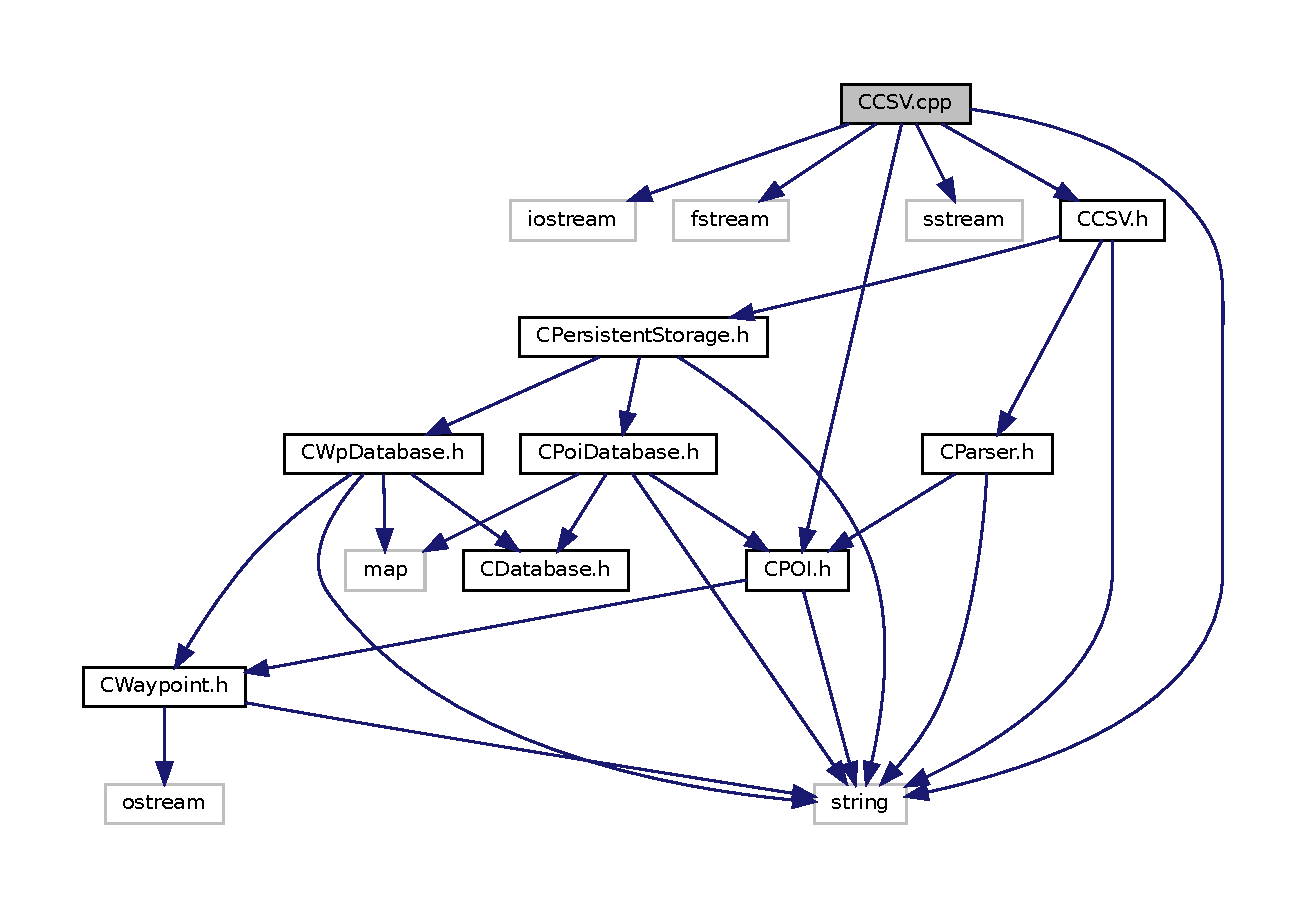
\includegraphics[width=350pt]{CCSV_8cpp__incl}
\end{center}
\end{figure}

\hypertarget{CCSV_8h}{}\section{C\+C\+S\+V.\+h File Reference}
\label{CCSV_8h}\index{C\+C\+S\+V.\+h@{C\+C\+S\+V.\+h}}
{\ttfamily \#include $<$string$>$}\newline
{\ttfamily \#include \char`\"{}C\+Persistent\+Storage.\+h\char`\"{}}\newline
{\ttfamily \#include \char`\"{}C\+Parser.\+h\char`\"{}}\newline
Include dependency graph for C\+C\+S\+V.\+h\+:
\nopagebreak
\begin{figure}[H]
\begin{center}
\leavevmode
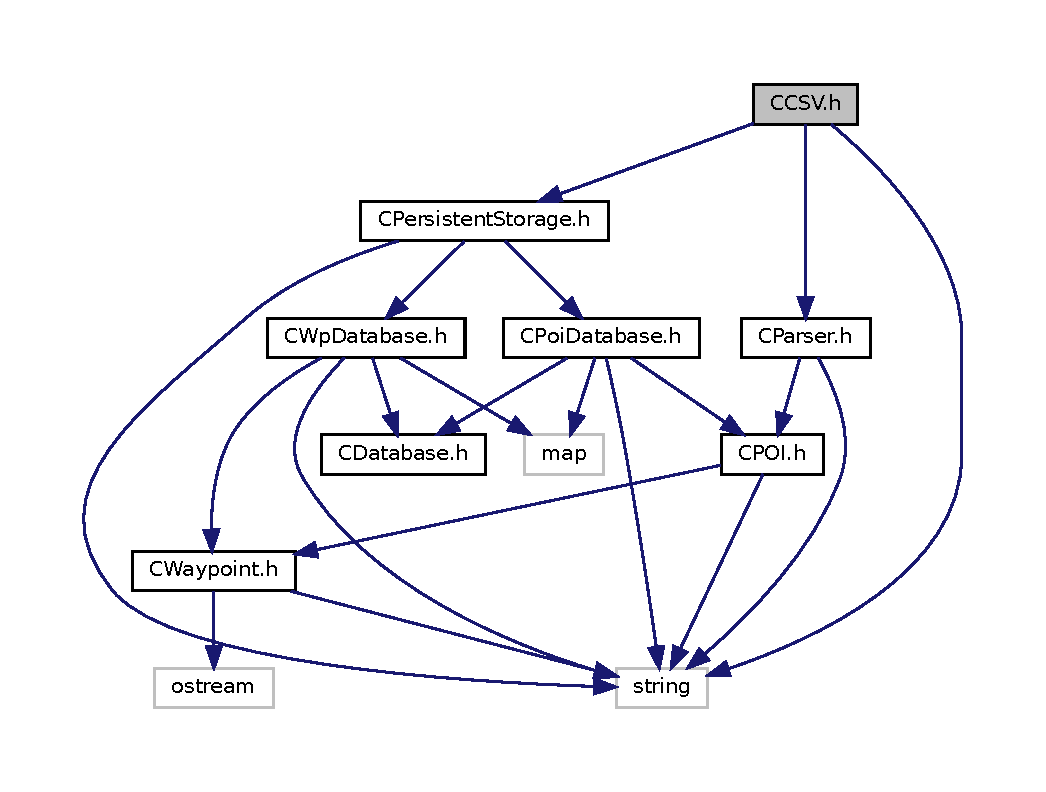
\includegraphics[width=350pt]{CCSV_8h__incl}
\end{center}
\end{figure}
This graph shows which files directly or indirectly include this file\+:
\nopagebreak
\begin{figure}[H]
\begin{center}
\leavevmode
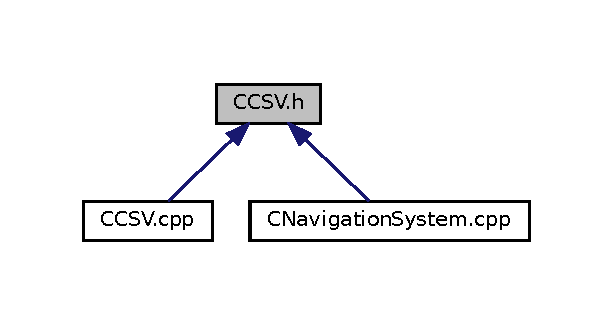
\includegraphics[width=294pt]{CCSV_8h__dep__incl}
\end{center}
\end{figure}
\subsection*{Classes}
\begin{DoxyCompactItemize}
\item 
class \hyperlink{classCCSV}{C\+C\+SV}
\end{DoxyCompactItemize}

\hypertarget{CDatabase_8h}{}\section{C\+Database.\+h File Reference}
\label{CDatabase_8h}\index{C\+Database.\+h@{C\+Database.\+h}}
This graph shows which files directly or indirectly include this file\+:
\nopagebreak
\begin{figure}[H]
\begin{center}
\leavevmode
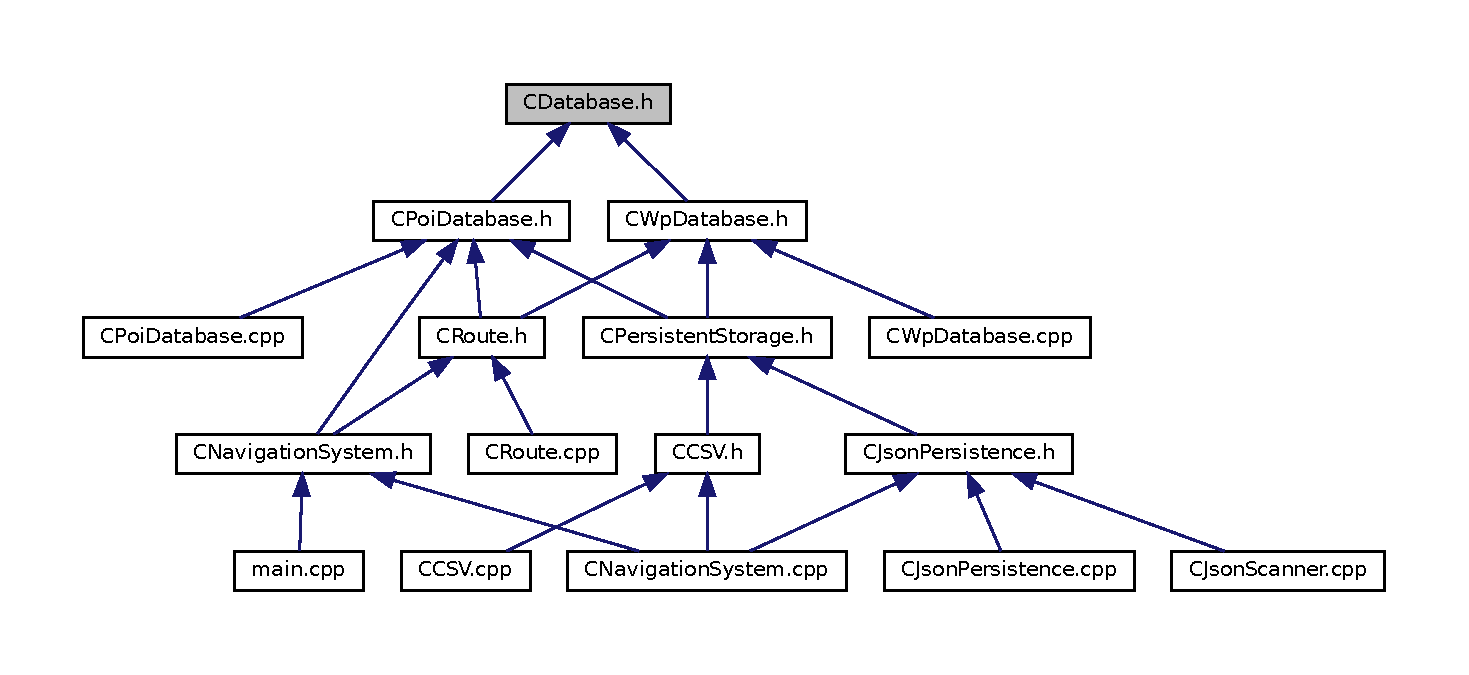
\includegraphics[width=350pt]{CDatabase_8h__dep__incl}
\end{center}
\end{figure}
\subsection*{Classes}
\begin{DoxyCompactItemize}
\item 
class \hyperlink{classCDatabase}{C\+Database$<$ T1, T2 $>$}
\end{DoxyCompactItemize}

\hypertarget{CGPSSensor_8cpp}{}\section{C\+G\+P\+S\+Sensor.\+cpp File Reference}
\label{CGPSSensor_8cpp}\index{C\+G\+P\+S\+Sensor.\+cpp@{C\+G\+P\+S\+Sensor.\+cpp}}
{\ttfamily \#include $<$iostream$>$}\newline
{\ttfamily \#include $<$limits$>$}\newline
{\ttfamily \#include \char`\"{}C\+G\+P\+S\+Sensor.\+h\char`\"{}}\newline
Include dependency graph for C\+G\+P\+S\+Sensor.\+cpp\+:
\nopagebreak
\begin{figure}[H]
\begin{center}
\leavevmode
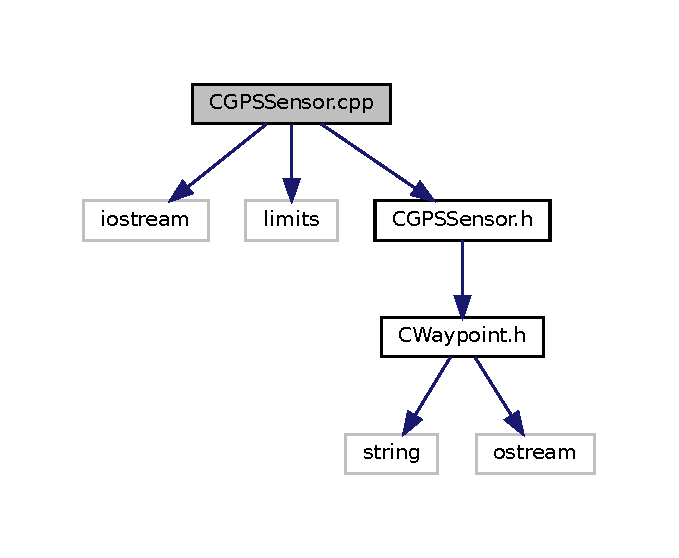
\includegraphics[width=326pt]{CGPSSensor_8cpp__incl}
\end{center}
\end{figure}

\hypertarget{CGPSSensor_8h}{}\section{C\+G\+P\+S\+Sensor.\+h File Reference}
\label{CGPSSensor_8h}\index{C\+G\+P\+S\+Sensor.\+h@{C\+G\+P\+S\+Sensor.\+h}}
{\ttfamily \#include \char`\"{}C\+Waypoint.\+h\char`\"{}}\newline
Include dependency graph for C\+G\+P\+S\+Sensor.\+h\+:
\nopagebreak
\begin{figure}[H]
\begin{center}
\leavevmode
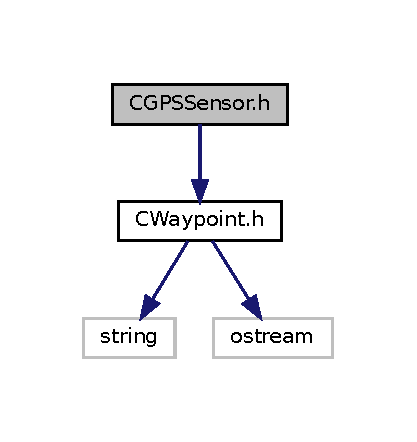
\includegraphics[width=200pt]{CGPSSensor_8h__incl}
\end{center}
\end{figure}
This graph shows which files directly or indirectly include this file\+:
\nopagebreak
\begin{figure}[H]
\begin{center}
\leavevmode
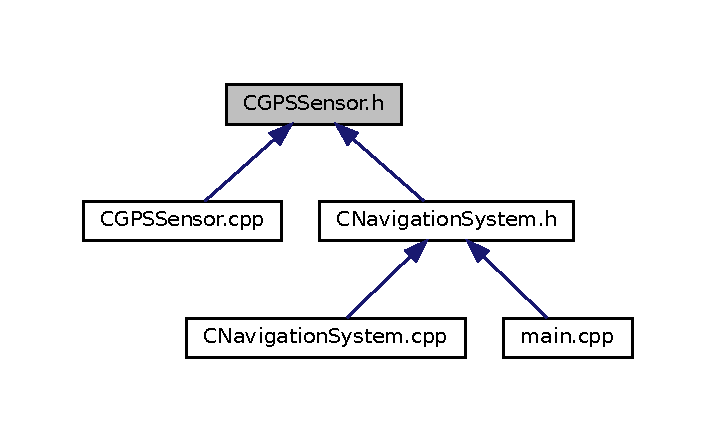
\includegraphics[width=344pt]{CGPSSensor_8h__dep__incl}
\end{center}
\end{figure}
\subsection*{Classes}
\begin{DoxyCompactItemize}
\item 
class \hyperlink{classCGPSSensor}{C\+G\+P\+S\+Sensor}
\end{DoxyCompactItemize}

\hypertarget{CJsonPersistence_8cpp}{}\section{C\+Json\+Persistence.\+cpp File Reference}
\label{CJsonPersistence_8cpp}\index{C\+Json\+Persistence.\+cpp@{C\+Json\+Persistence.\+cpp}}
{\ttfamily \#include $<$iostream$>$}\newline
{\ttfamily \#include $<$fstream$>$}\newline
{\ttfamily \#include $<$string$>$}\newline
{\ttfamily \#include $<$sstream$>$}\newline
{\ttfamily \#include \char`\"{}C\+P\+O\+I.\+h\char`\"{}}\newline
{\ttfamily \#include \char`\"{}C\+Json\+Persistence.\+h\char`\"{}}\newline
Include dependency graph for C\+Json\+Persistence.\+cpp\+:
\nopagebreak
\begin{figure}[H]
\begin{center}
\leavevmode
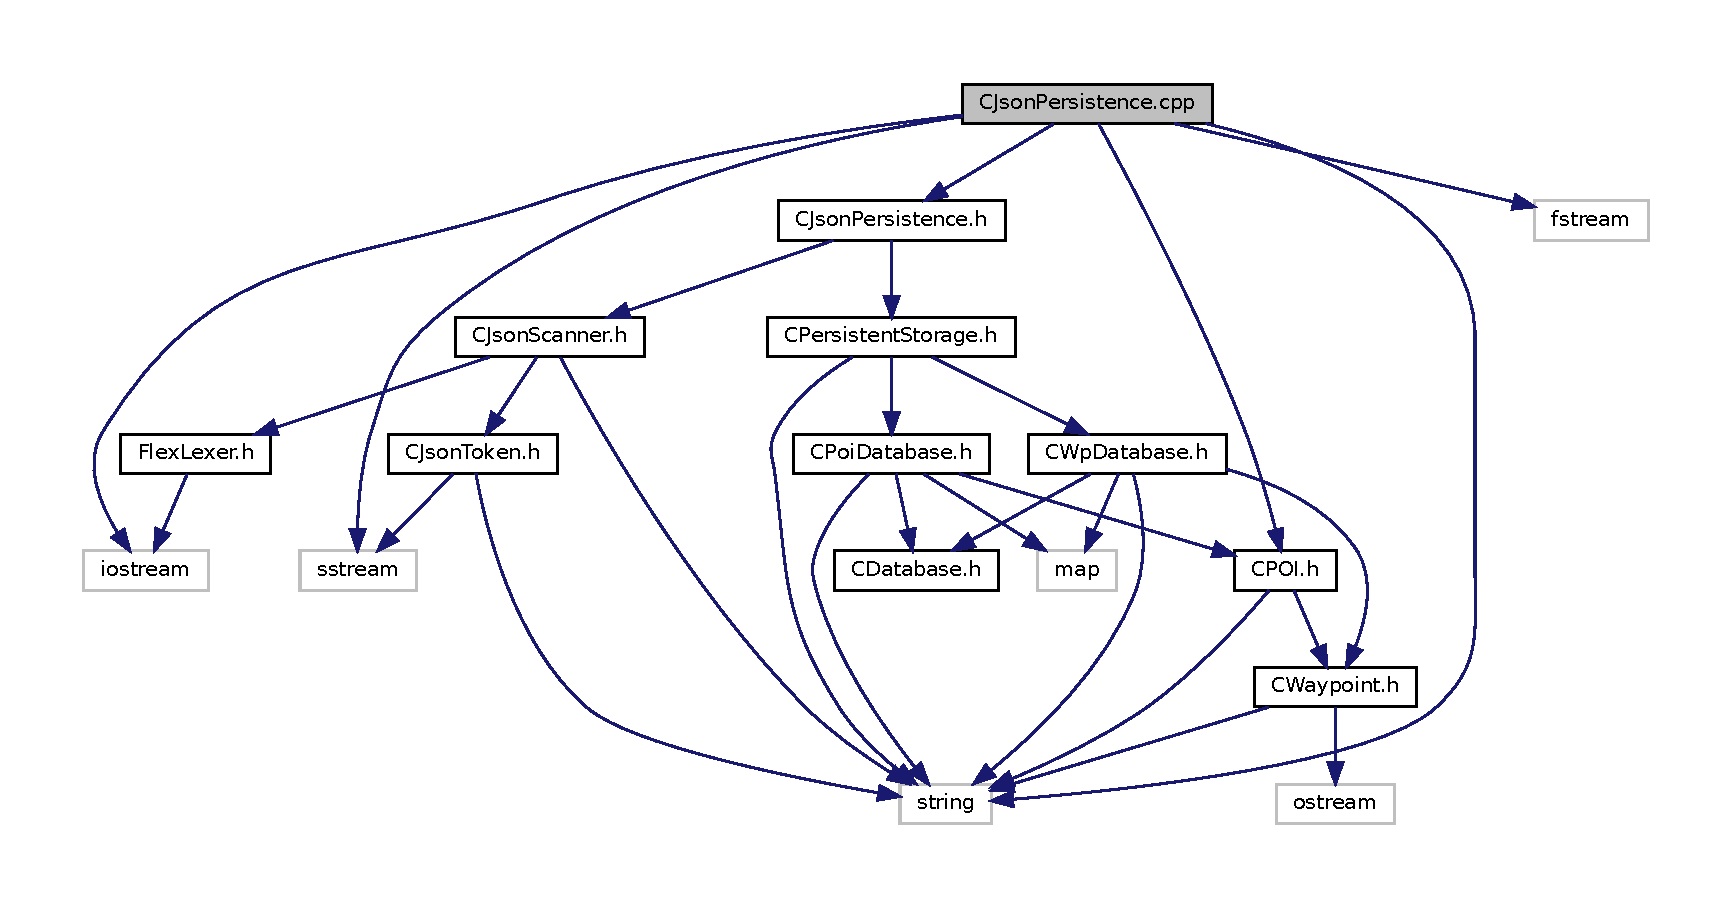
\includegraphics[width=350pt]{CJsonPersistence_8cpp__incl}
\end{center}
\end{figure}

\hypertarget{CJsonPersistence_8h}{}\section{C\+Json\+Persistence.\+h File Reference}
\label{CJsonPersistence_8h}\index{C\+Json\+Persistence.\+h@{C\+Json\+Persistence.\+h}}
{\ttfamily \#include \char`\"{}C\+Json\+Scanner.\+h\char`\"{}}\newline
{\ttfamily \#include \char`\"{}C\+Persistent\+Storage.\+h\char`\"{}}\newline
Include dependency graph for C\+Json\+Persistence.\+h\+:
\nopagebreak
\begin{figure}[H]
\begin{center}
\leavevmode
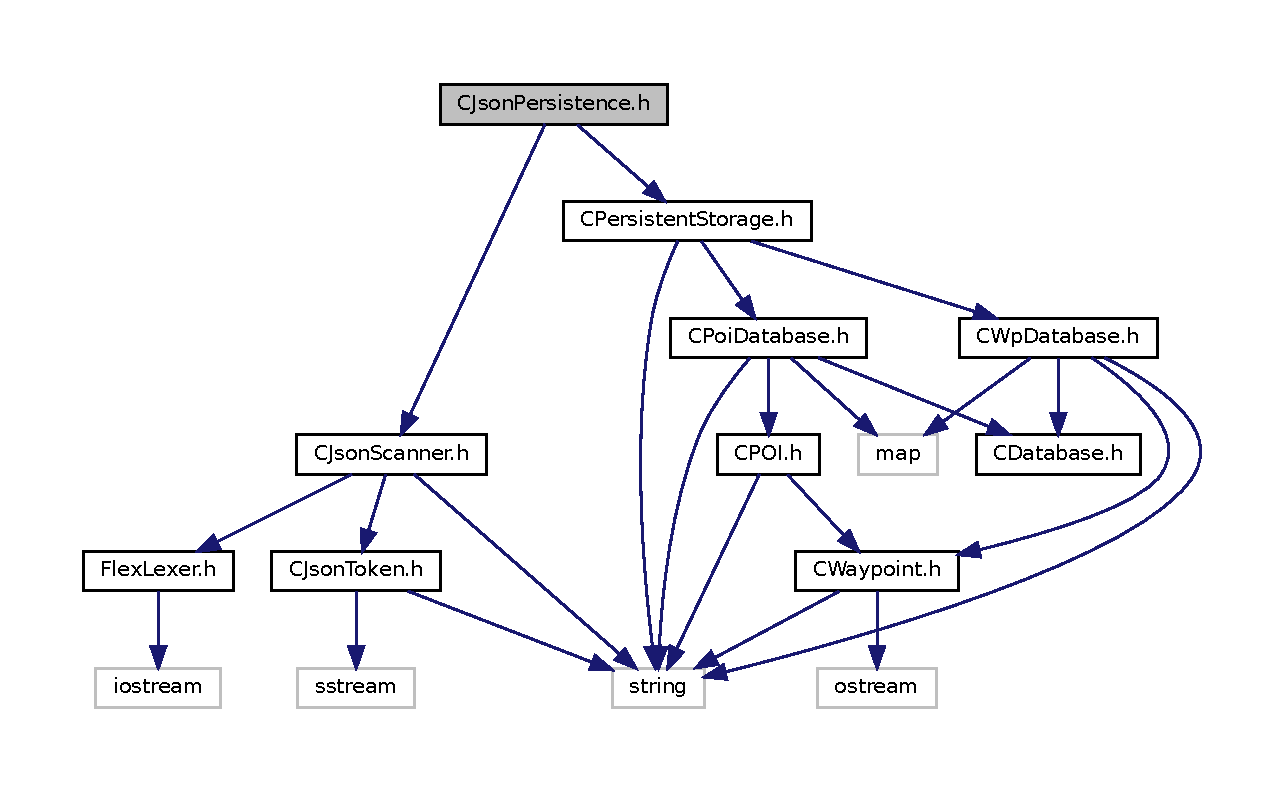
\includegraphics[width=350pt]{CJsonPersistence_8h__incl}
\end{center}
\end{figure}
This graph shows which files directly or indirectly include this file\+:
\nopagebreak
\begin{figure}[H]
\begin{center}
\leavevmode
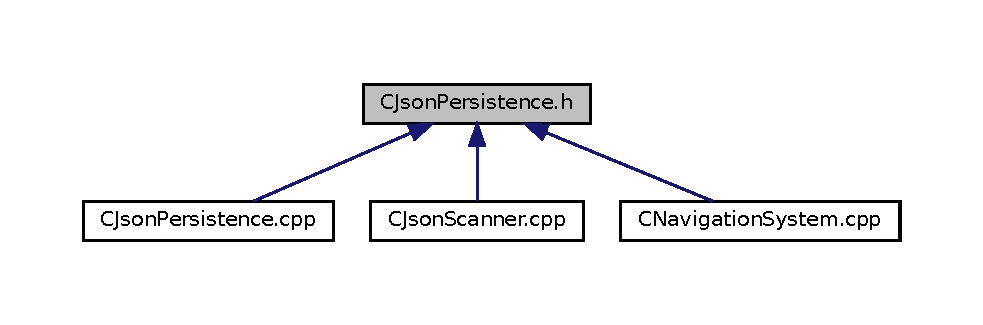
\includegraphics[width=350pt]{CJsonPersistence_8h__dep__incl}
\end{center}
\end{figure}
\subsection*{Classes}
\begin{DoxyCompactItemize}
\item 
class \hyperlink{classCJsonPersistence}{C\+Json\+Persistence}
\end{DoxyCompactItemize}

\hypertarget{CJsonScanner_8cpp}{}\section{C\+Json\+Scanner.\+cpp File Reference}
\label{CJsonScanner_8cpp}\index{C\+Json\+Scanner.\+cpp@{C\+Json\+Scanner.\+cpp}}
{\ttfamily \#include $<$string$>$}\newline
{\ttfamily \#include \char`\"{}C\+Json\+Scanner.\+h\char`\"{}}\newline
{\ttfamily \#include \char`\"{}C\+Json\+Persistence.\+h\char`\"{}}\newline
Include dependency graph for C\+Json\+Scanner.\+cpp\+:
\nopagebreak
\begin{figure}[H]
\begin{center}
\leavevmode
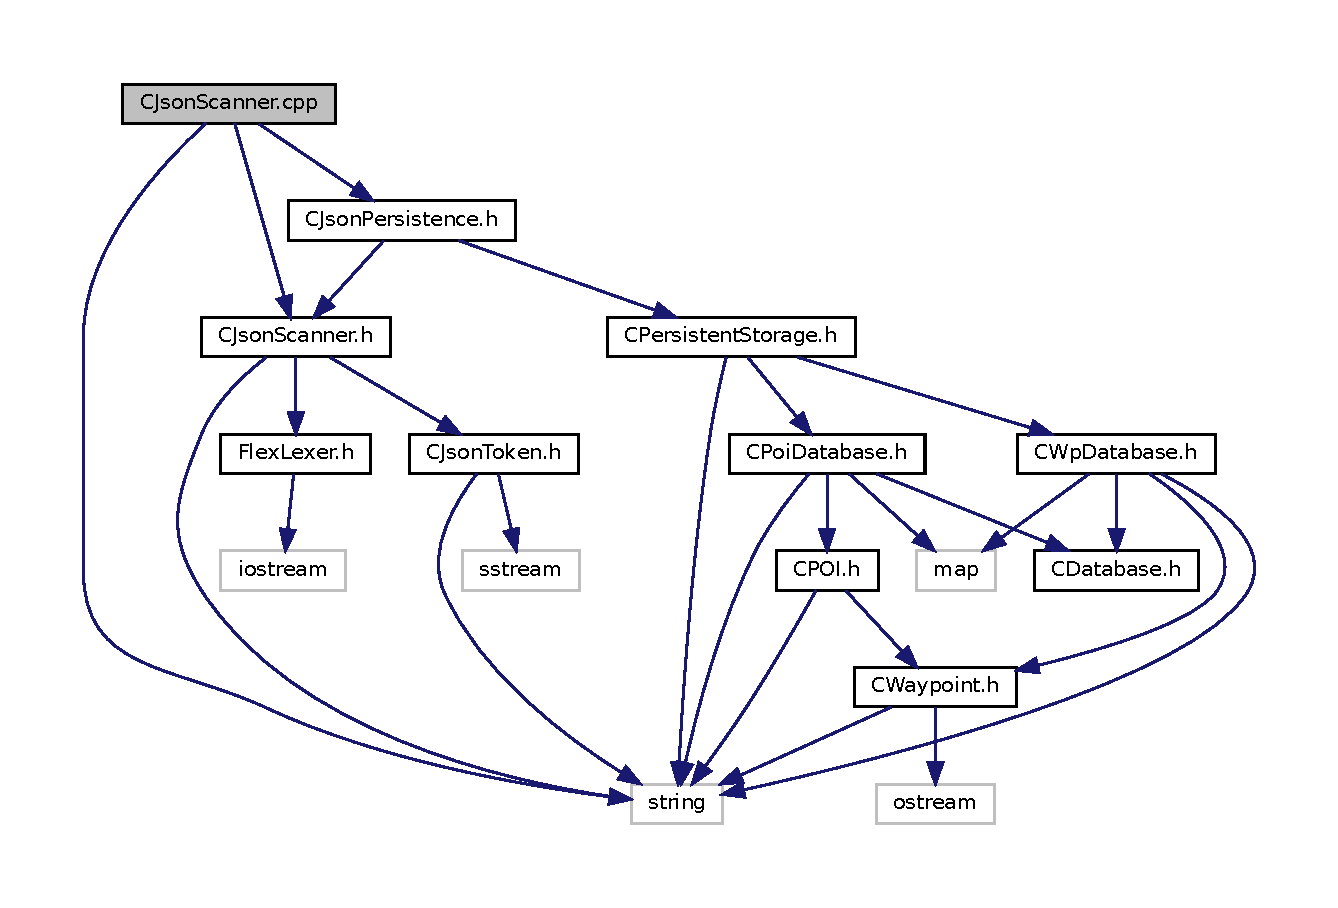
\includegraphics[width=350pt]{CJsonScanner_8cpp__incl}
\end{center}
\end{figure}
\subsection*{Namespaces}
\begin{DoxyCompactItemize}
\item 
 \hyperlink{namespaceAPT}{A\+PT}
\end{DoxyCompactItemize}

\hypertarget{CJsonScanner_8h}{}\section{C\+Json\+Scanner.\+h File Reference}
\label{CJsonScanner_8h}\index{C\+Json\+Scanner.\+h@{C\+Json\+Scanner.\+h}}
{\ttfamily \#include $<$string$>$}\newline
{\ttfamily \#include \char`\"{}Flex\+Lexer.\+h\char`\"{}}\newline
{\ttfamily \#include \char`\"{}C\+Json\+Token.\+h\char`\"{}}\newline
Include dependency graph for C\+Json\+Scanner.\+h\+:
\nopagebreak
\begin{figure}[H]
\begin{center}
\leavevmode
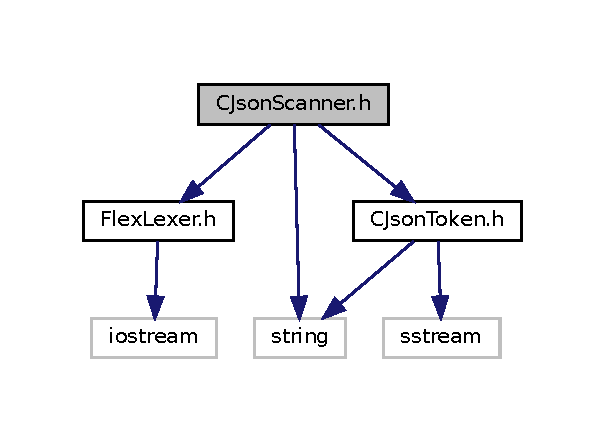
\includegraphics[width=291pt]{CJsonScanner_8h__incl}
\end{center}
\end{figure}
This graph shows which files directly or indirectly include this file\+:
\nopagebreak
\begin{figure}[H]
\begin{center}
\leavevmode
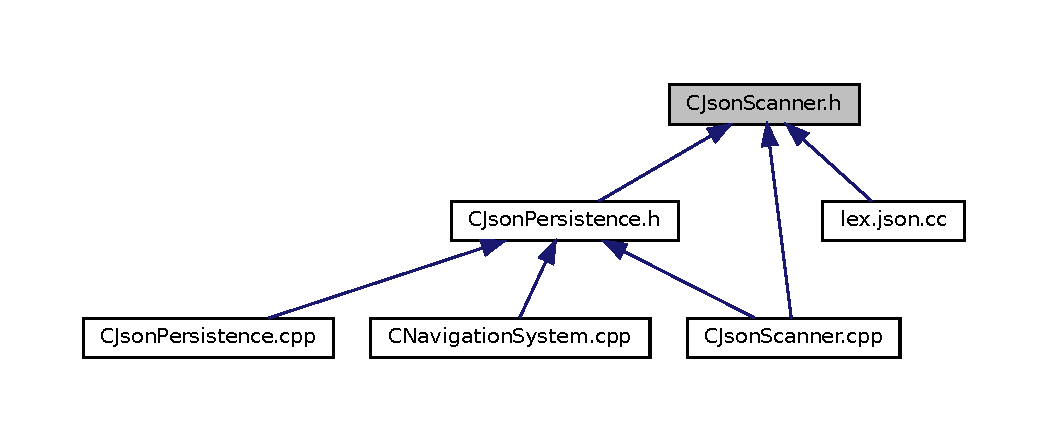
\includegraphics[width=350pt]{CJsonScanner_8h__dep__incl}
\end{center}
\end{figure}
\subsection*{Classes}
\begin{DoxyCompactItemize}
\item 
class \hyperlink{classAPT_1_1CJsonScanner}{A\+P\+T\+::\+C\+Json\+Scanner}
\end{DoxyCompactItemize}
\subsection*{Namespaces}
\begin{DoxyCompactItemize}
\item 
 \hyperlink{namespaceAPT}{A\+PT}
\end{DoxyCompactItemize}
\subsection*{Macros}
\begin{DoxyCompactItemize}
\item 
\#define \hyperlink{CJsonScanner_8h_af699458ba5331ddec7e15a878f42f8f5}{yy\+Flex\+Lexer}~json\+Flex\+Lexer
\end{DoxyCompactItemize}


\subsection{Macro Definition Documentation}
\mbox{\Hypertarget{CJsonScanner_8h_af699458ba5331ddec7e15a878f42f8f5}\label{CJsonScanner_8h_af699458ba5331ddec7e15a878f42f8f5}} 
\index{C\+Json\+Scanner.\+h@{C\+Json\+Scanner.\+h}!yy\+Flex\+Lexer@{yy\+Flex\+Lexer}}
\index{yy\+Flex\+Lexer@{yy\+Flex\+Lexer}!C\+Json\+Scanner.\+h@{C\+Json\+Scanner.\+h}}
\subsubsection{\texorpdfstring{yy\+Flex\+Lexer}{yyFlexLexer}}
{\footnotesize\ttfamily \#define \hyperlink{classyyFlexLexer}{yy\+Flex\+Lexer}~json\+Flex\+Lexer}


\hypertarget{CJsonToken_8cpp}{}\section{C\+Json\+Token.\+cpp File Reference}
\label{CJsonToken_8cpp}\index{C\+Json\+Token.\+cpp@{C\+Json\+Token.\+cpp}}
{\ttfamily \#include \char`\"{}C\+Json\+Token.\+h\char`\"{}}\newline
Include dependency graph for C\+Json\+Token.\+cpp\+:
\nopagebreak
\begin{figure}[H]
\begin{center}
\leavevmode
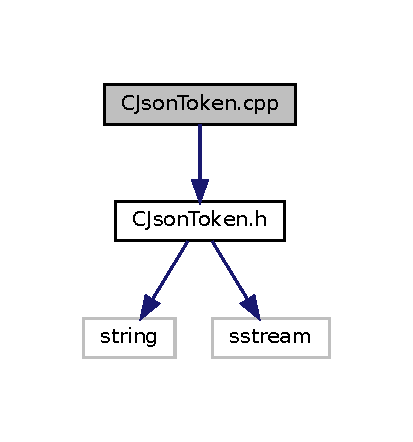
\includegraphics[width=198pt]{CJsonToken_8cpp__incl}
\end{center}
\end{figure}
\subsection*{Namespaces}
\begin{DoxyCompactItemize}
\item 
 \hyperlink{namespaceAPT}{A\+PT}
\end{DoxyCompactItemize}

\hypertarget{CJsonToken_8h}{}\section{C\+Json\+Token.\+h File Reference}
\label{CJsonToken_8h}\index{C\+Json\+Token.\+h@{C\+Json\+Token.\+h}}
{\ttfamily \#include $<$string$>$}\newline
{\ttfamily \#include $<$sstream$>$}\newline
Include dependency graph for C\+Json\+Token.\+h\+:
\nopagebreak
\begin{figure}[H]
\begin{center}
\leavevmode
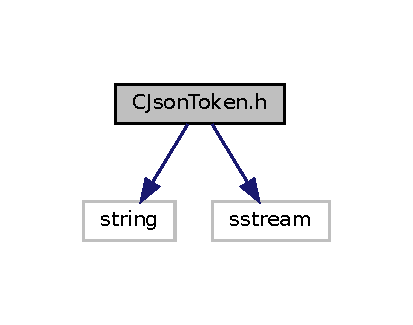
\includegraphics[width=198pt]{CJsonToken_8h__incl}
\end{center}
\end{figure}
This graph shows which files directly or indirectly include this file\+:
\nopagebreak
\begin{figure}[H]
\begin{center}
\leavevmode
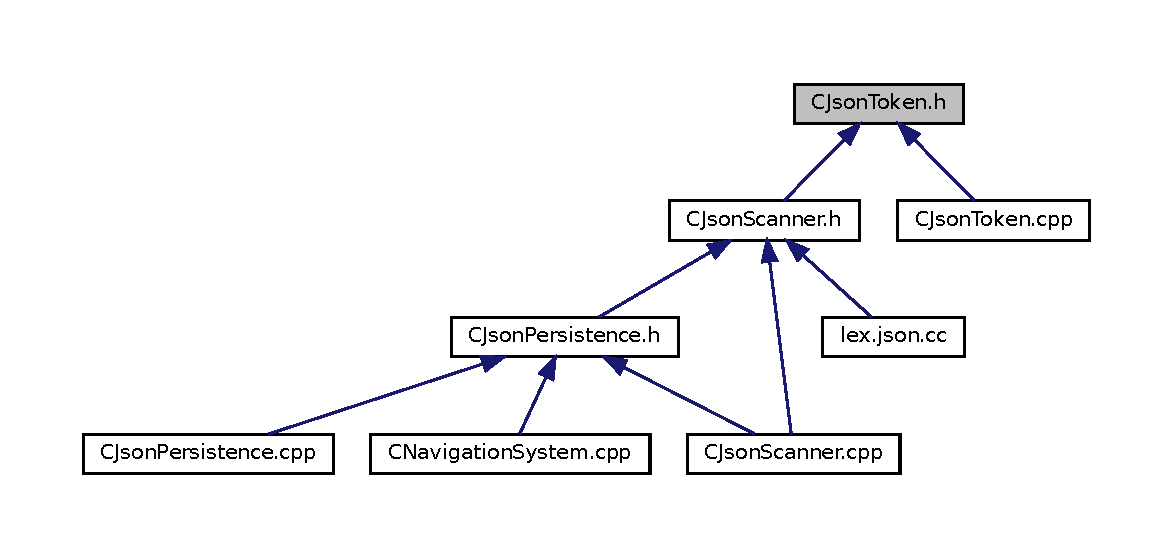
\includegraphics[width=350pt]{CJsonToken_8h__dep__incl}
\end{center}
\end{figure}
\subsection*{Classes}
\begin{DoxyCompactItemize}
\item 
class \hyperlink{classAPT_1_1CJsonToken}{A\+P\+T\+::\+C\+Json\+Token}
\item 
class \hyperlink{classAPT_1_1CJsonValueToken}{A\+P\+T\+::\+C\+Json\+Value\+Token$<$ token\+Type, T $>$}
\end{DoxyCompactItemize}
\subsection*{Namespaces}
\begin{DoxyCompactItemize}
\item 
 \hyperlink{namespaceAPT}{A\+PT}
\end{DoxyCompactItemize}
\subsection*{Typedefs}
\begin{DoxyCompactItemize}
\item 
typedef C\+Json\+Value\+Token$<$ C\+Json\+Token\+::\+S\+T\+R\+I\+NG, std\+::string $>$ \hyperlink{namespaceAPT_a3af7abde9f907425ef65954a9b102083}{A\+P\+T\+::\+C\+Json\+String\+Token}
\item 
typedef C\+Json\+Value\+Token$<$ C\+Json\+Token\+::\+N\+U\+M\+B\+ER, double $>$ \hyperlink{namespaceAPT_aacc16da16d083aefa789bc0198b3effd}{A\+P\+T\+::\+C\+Json\+Number\+Token}
\item 
typedef C\+Json\+Value\+Token$<$ C\+Json\+Token\+::\+B\+O\+OL, bool $>$ \hyperlink{namespaceAPT_a6f531ac7001387df5b08e93d8f586000}{A\+P\+T\+::\+C\+Json\+Bool\+Token}
\end{DoxyCompactItemize}

\hypertarget{CNavigationSystem_8cpp}{}\section{C\+Navigation\+System.\+cpp File Reference}
\label{CNavigationSystem_8cpp}\index{C\+Navigation\+System.\+cpp@{C\+Navigation\+System.\+cpp}}
{\ttfamily \#include $<$iostream$>$}\newline
{\ttfamily \#include \char`\"{}C\+Navigation\+System.\+h\char`\"{}}\newline
{\ttfamily \#include \char`\"{}C\+C\+S\+V.\+h\char`\"{}}\newline
{\ttfamily \#include \char`\"{}C\+Json\+Persistence.\+h\char`\"{}}\newline
Include dependency graph for C\+Navigation\+System.\+cpp\+:
\nopagebreak
\begin{figure}[H]
\begin{center}
\leavevmode
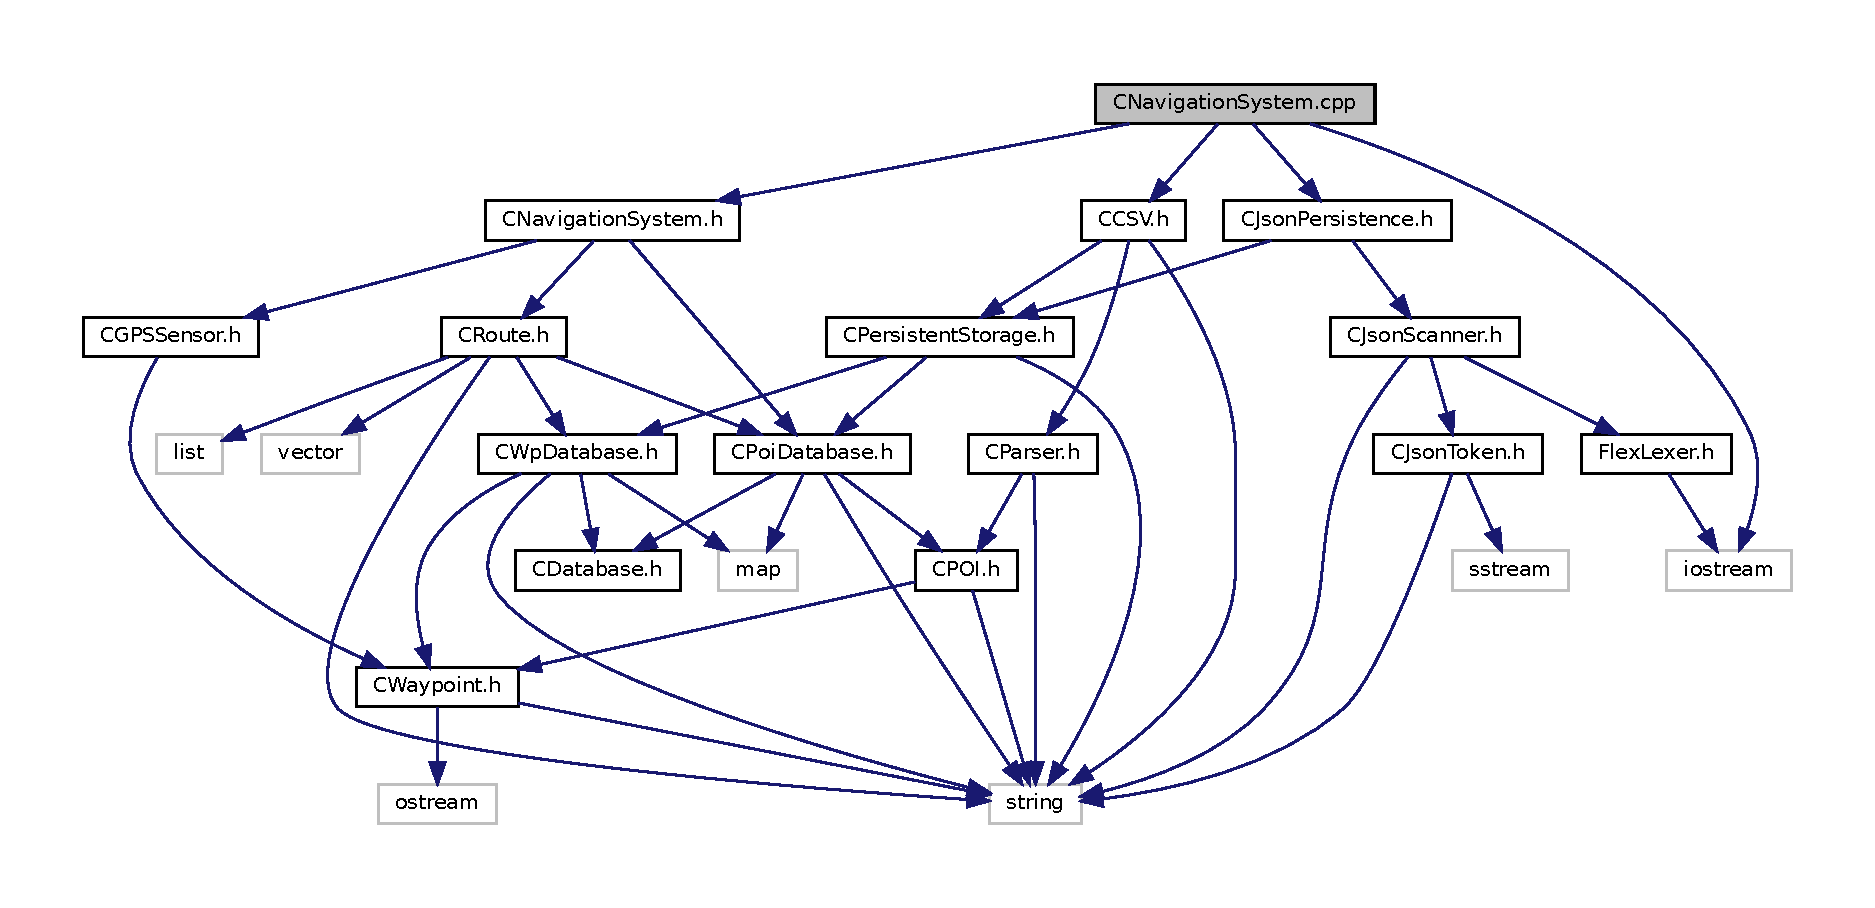
\includegraphics[width=350pt]{CNavigationSystem_8cpp__incl}
\end{center}
\end{figure}
\subsection*{Macros}
\begin{DoxyCompactItemize}
\item 
\#define \hyperlink{CNavigationSystem_8cpp_a3dfc1a58a44b3134950d286c4d5b59a2}{C\+SV}~0
\item 
\#define \hyperlink{CNavigationSystem_8cpp_a730e2c2c514ed61217dabd3a78a99d8d}{J\+S\+ON}~1
\item 
\#define \hyperlink{CNavigationSystem_8cpp_a161a8badd2ae83b4071c10486aa4da87}{C\+O\+N\+F\+I\+G\+\_\+\+P\+E\+R\+S\+I\+S\+T\+E\+N\+C\+E\+\_\+\+S\+T\+O\+R\+A\+GE}~\hyperlink{CNavigationSystem_8cpp_a730e2c2c514ed61217dabd3a78a99d8d}{J\+S\+ON}
\end{DoxyCompactItemize}


\subsection{Macro Definition Documentation}
\mbox{\Hypertarget{CNavigationSystem_8cpp_a161a8badd2ae83b4071c10486aa4da87}\label{CNavigationSystem_8cpp_a161a8badd2ae83b4071c10486aa4da87}} 
\index{C\+Navigation\+System.\+cpp@{C\+Navigation\+System.\+cpp}!C\+O\+N\+F\+I\+G\+\_\+\+P\+E\+R\+S\+I\+S\+T\+E\+N\+C\+E\+\_\+\+S\+T\+O\+R\+A\+GE@{C\+O\+N\+F\+I\+G\+\_\+\+P\+E\+R\+S\+I\+S\+T\+E\+N\+C\+E\+\_\+\+S\+T\+O\+R\+A\+GE}}
\index{C\+O\+N\+F\+I\+G\+\_\+\+P\+E\+R\+S\+I\+S\+T\+E\+N\+C\+E\+\_\+\+S\+T\+O\+R\+A\+GE@{C\+O\+N\+F\+I\+G\+\_\+\+P\+E\+R\+S\+I\+S\+T\+E\+N\+C\+E\+\_\+\+S\+T\+O\+R\+A\+GE}!C\+Navigation\+System.\+cpp@{C\+Navigation\+System.\+cpp}}
\subsubsection{\texorpdfstring{C\+O\+N\+F\+I\+G\+\_\+\+P\+E\+R\+S\+I\+S\+T\+E\+N\+C\+E\+\_\+\+S\+T\+O\+R\+A\+GE}{CONFIG\_PERSISTENCE\_STORAGE}}
{\footnotesize\ttfamily \#define C\+O\+N\+F\+I\+G\+\_\+\+P\+E\+R\+S\+I\+S\+T\+E\+N\+C\+E\+\_\+\+S\+T\+O\+R\+A\+GE~\hyperlink{CNavigationSystem_8cpp_a730e2c2c514ed61217dabd3a78a99d8d}{J\+S\+ON}}

\mbox{\Hypertarget{CNavigationSystem_8cpp_a3dfc1a58a44b3134950d286c4d5b59a2}\label{CNavigationSystem_8cpp_a3dfc1a58a44b3134950d286c4d5b59a2}} 
\index{C\+Navigation\+System.\+cpp@{C\+Navigation\+System.\+cpp}!C\+SV@{C\+SV}}
\index{C\+SV@{C\+SV}!C\+Navigation\+System.\+cpp@{C\+Navigation\+System.\+cpp}}
\subsubsection{\texorpdfstring{C\+SV}{CSV}}
{\footnotesize\ttfamily \#define C\+SV~0}

\mbox{\Hypertarget{CNavigationSystem_8cpp_a730e2c2c514ed61217dabd3a78a99d8d}\label{CNavigationSystem_8cpp_a730e2c2c514ed61217dabd3a78a99d8d}} 
\index{C\+Navigation\+System.\+cpp@{C\+Navigation\+System.\+cpp}!J\+S\+ON@{J\+S\+ON}}
\index{J\+S\+ON@{J\+S\+ON}!C\+Navigation\+System.\+cpp@{C\+Navigation\+System.\+cpp}}
\subsubsection{\texorpdfstring{J\+S\+ON}{JSON}}
{\footnotesize\ttfamily \#define J\+S\+ON~1}


\hypertarget{CNavigationSystem_8h}{}\section{C\+Navigation\+System.\+h File Reference}
\label{CNavigationSystem_8h}\index{C\+Navigation\+System.\+h@{C\+Navigation\+System.\+h}}
{\ttfamily \#include \char`\"{}C\+G\+P\+S\+Sensor.\+h\char`\"{}}\newline
{\ttfamily \#include \char`\"{}C\+Route.\+h\char`\"{}}\newline
{\ttfamily \#include \char`\"{}C\+Poi\+Database.\+h\char`\"{}}\newline
Include dependency graph for C\+Navigation\+System.\+h\+:
\nopagebreak
\begin{figure}[H]
\begin{center}
\leavevmode
\includegraphics[width=350pt]{CNavigationSystem_8h__incl}
\end{center}
\end{figure}
This graph shows which files directly or indirectly include this file\+:
\nopagebreak
\begin{figure}[H]
\begin{center}
\leavevmode
\includegraphics[width=294pt]{CNavigationSystem_8h__dep__incl}
\end{center}
\end{figure}
\subsection*{Classes}
\begin{DoxyCompactItemize}
\item 
class \hyperlink{classCNavigationSystem}{C\+Navigation\+System}
\end{DoxyCompactItemize}

\hypertarget{CParser_8cpp}{}\section{C\+Parser.\+cpp File Reference}
\label{CParser_8cpp}\index{C\+Parser.\+cpp@{C\+Parser.\+cpp}}
{\ttfamily \#include $<$iostream$>$}\newline
{\ttfamily \#include $<$fstream$>$}\newline
{\ttfamily \#include $<$string$>$}\newline
{\ttfamily \#include $<$sstream$>$}\newline
{\ttfamily \#include \char`\"{}C\+Parser.\+h\char`\"{}}\newline
Include dependency graph for C\+Parser.\+cpp\+:
\nopagebreak
\begin{figure}[H]
\begin{center}
\leavevmode
\includegraphics[width=350pt]{CParser_8cpp__incl}
\end{center}
\end{figure}

\hypertarget{CParser_8h}{}\section{C\+Parser.\+h File Reference}
\label{CParser_8h}\index{C\+Parser.\+h@{C\+Parser.\+h}}
{\ttfamily \#include $<$string$>$}\newline
{\ttfamily \#include \char`\"{}C\+P\+O\+I.\+h\char`\"{}}\newline
Include dependency graph for C\+Parser.\+h\+:
\nopagebreak
\begin{figure}[H]
\begin{center}
\leavevmode
\includegraphics[width=229pt]{CParser_8h__incl}
\end{center}
\end{figure}
This graph shows which files directly or indirectly include this file\+:
\nopagebreak
\begin{figure}[H]
\begin{center}
\leavevmode
\includegraphics[width=294pt]{CParser_8h__dep__incl}
\end{center}
\end{figure}
\subsection*{Classes}
\begin{DoxyCompactItemize}
\item 
class \hyperlink{classCParser}{C\+Parser}
\end{DoxyCompactItemize}

\hypertarget{CPersistentStorage_8h}{}\section{C\+Persistent\+Storage.\+h File Reference}
\label{CPersistentStorage_8h}\index{C\+Persistent\+Storage.\+h@{C\+Persistent\+Storage.\+h}}
{\ttfamily \#include $<$string$>$}\newline
{\ttfamily \#include \char`\"{}C\+Poi\+Database.\+h\char`\"{}}\newline
{\ttfamily \#include \char`\"{}C\+Wp\+Database.\+h\char`\"{}}\newline
Include dependency graph for C\+Persistent\+Storage.\+h\+:
\nopagebreak
\begin{figure}[H]
\begin{center}
\leavevmode
\includegraphics[width=350pt]{CPersistentStorage_8h__incl}
\end{center}
\end{figure}
This graph shows which files directly or indirectly include this file\+:
\nopagebreak
\begin{figure}[H]
\begin{center}
\leavevmode
\includegraphics[width=350pt]{CPersistentStorage_8h__dep__incl}
\end{center}
\end{figure}
\subsection*{Classes}
\begin{DoxyCompactItemize}
\item 
class \hyperlink{classCPersistentStorage}{C\+Persistent\+Storage}
\end{DoxyCompactItemize}

\hypertarget{CPOI_8cpp}{}\section{C\+P\+O\+I.\+cpp File Reference}
\label{CPOI_8cpp}\index{C\+P\+O\+I.\+cpp@{C\+P\+O\+I.\+cpp}}
{\ttfamily \#include $<$iostream$>$}\newline
{\ttfamily \#include $<$string$>$}\newline
{\ttfamily \#include \char`\"{}C\+P\+O\+I.\+h\char`\"{}}\newline
Include dependency graph for C\+P\+O\+I.\+cpp\+:
\nopagebreak
\begin{figure}[H]
\begin{center}
\leavevmode
\includegraphics[width=312pt]{CPOI_8cpp__incl}
\end{center}
\end{figure}
\subsection*{Classes}
\begin{DoxyCompactItemize}
\item 
struct \hyperlink{structPOITypeName}{P\+O\+I\+Type\+Name}
\end{DoxyCompactItemize}
\subsection*{Functions}
\begin{DoxyCompactItemize}
\item 
ostream \& \hyperlink{CPOI_8cpp_a37a0622d27e0bfcb12be83f65a7c72fd}{operator$<$$<$} (ostream \&stream, \hyperlink{classCPOI}{C\+P\+OI} const \&poi)
\end{DoxyCompactItemize}


\subsection{Function Documentation}
\mbox{\Hypertarget{CPOI_8cpp_a37a0622d27e0bfcb12be83f65a7c72fd}\label{CPOI_8cpp_a37a0622d27e0bfcb12be83f65a7c72fd}} 
\index{C\+P\+O\+I.\+cpp@{C\+P\+O\+I.\+cpp}!operator$<$$<$@{operator$<$$<$}}
\index{operator$<$$<$@{operator$<$$<$}!C\+P\+O\+I.\+cpp@{C\+P\+O\+I.\+cpp}}
\subsubsection{\texorpdfstring{operator$<$$<$()}{operator<<()}}
{\footnotesize\ttfamily ostream\& operator$<$$<$ (\begin{DoxyParamCaption}\item[{ostream \&}]{stream,  }\item[{\hyperlink{classCPOI}{C\+P\+OI} const \&}]{poi }\end{DoxyParamCaption})}

An operator overloaded friend function which prints the P\+OI information param@ ostream \&stream -\/ output stream (I\+N/\+O\+UT) param@ \hyperlink{classCPOI}{C\+P\+OI} const \&poi -\/ A P\+OI (IN) returnvalue@ output stream with the P\+OI information 
\hypertarget{CPOI_8h}{}\section{C\+P\+O\+I.\+h File Reference}
\label{CPOI_8h}\index{C\+P\+O\+I.\+h@{C\+P\+O\+I.\+h}}
{\ttfamily \#include $<$string$>$}\newline
{\ttfamily \#include \char`\"{}C\+Waypoint.\+h\char`\"{}}\newline
Include dependency graph for C\+P\+O\+I.\+h\+:
\nopagebreak
\begin{figure}[H]
\begin{center}
\leavevmode
\includegraphics[width=208pt]{CPOI_8h__incl}
\end{center}
\end{figure}
This graph shows which files directly or indirectly include this file\+:
\nopagebreak
\begin{figure}[H]
\begin{center}
\leavevmode
\includegraphics[width=350pt]{CPOI_8h__dep__incl}
\end{center}
\end{figure}
\subsection*{Classes}
\begin{DoxyCompactItemize}
\item 
class \hyperlink{classCPOI}{C\+P\+OI}
\end{DoxyCompactItemize}

\hypertarget{CPoiDatabase_8cpp}{}\section{C\+Poi\+Database.\+cpp File Reference}
\label{CPoiDatabase_8cpp}\index{C\+Poi\+Database.\+cpp@{C\+Poi\+Database.\+cpp}}
{\ttfamily \#include $<$iostream$>$}\newline
{\ttfamily \#include \char`\"{}C\+Poi\+Database.\+h\char`\"{}}\newline
Include dependency graph for C\+Poi\+Database.\+cpp\+:
\nopagebreak
\begin{figure}[H]
\begin{center}
\leavevmode
\includegraphics[width=350pt]{CPoiDatabase_8cpp__incl}
\end{center}
\end{figure}

\hypertarget{CPoiDatabase_8h}{}\section{C\+Poi\+Database.\+h File Reference}
\label{CPoiDatabase_8h}\index{C\+Poi\+Database.\+h@{C\+Poi\+Database.\+h}}
{\ttfamily \#include $<$string$>$}\newline
{\ttfamily \#include $<$map$>$}\newline
{\ttfamily \#include \char`\"{}C\+P\+O\+I.\+h\char`\"{}}\newline
{\ttfamily \#include \char`\"{}C\+Database.\+h\char`\"{}}\newline
Include dependency graph for C\+Poi\+Database.\+h\+:
\nopagebreak
\begin{figure}[H]
\begin{center}
\leavevmode
\includegraphics[width=299pt]{CPoiDatabase_8h__incl}
\end{center}
\end{figure}
This graph shows which files directly or indirectly include this file\+:
\nopagebreak
\begin{figure}[H]
\begin{center}
\leavevmode
\includegraphics[width=350pt]{CPoiDatabase_8h__dep__incl}
\end{center}
\end{figure}
\subsection*{Classes}
\begin{DoxyCompactItemize}
\item 
class \hyperlink{classCPoiDatabase}{C\+Poi\+Database}
\end{DoxyCompactItemize}
\subsection*{Typedefs}
\begin{DoxyCompactItemize}
\item 
typedef std\+::string \hyperlink{CPoiDatabase_8h_ad55418fc31c1491ccfbd50da54f494a0}{P\+O\+I\+\_\+\+Database\+\_\+key\+\_\+t}
\end{DoxyCompactItemize}


\subsection{Typedef Documentation}
\mbox{\Hypertarget{CPoiDatabase_8h_ad55418fc31c1491ccfbd50da54f494a0}\label{CPoiDatabase_8h_ad55418fc31c1491ccfbd50da54f494a0}} 
\index{C\+Poi\+Database.\+h@{C\+Poi\+Database.\+h}!P\+O\+I\+\_\+\+Database\+\_\+key\+\_\+t@{P\+O\+I\+\_\+\+Database\+\_\+key\+\_\+t}}
\index{P\+O\+I\+\_\+\+Database\+\_\+key\+\_\+t@{P\+O\+I\+\_\+\+Database\+\_\+key\+\_\+t}!C\+Poi\+Database.\+h@{C\+Poi\+Database.\+h}}
\subsubsection{\texorpdfstring{P\+O\+I\+\_\+\+Database\+\_\+key\+\_\+t}{POI\_Database\_key\_t}}
{\footnotesize\ttfamily typedef std\+::string \hyperlink{CPoiDatabase_8h_ad55418fc31c1491ccfbd50da54f494a0}{P\+O\+I\+\_\+\+Database\+\_\+key\+\_\+t}}


\hypertarget{CRoute_8cpp}{}\section{C\+Route.\+cpp File Reference}
\label{CRoute_8cpp}\index{C\+Route.\+cpp@{C\+Route.\+cpp}}
{\ttfamily \#include $<$iostream$>$}\newline
{\ttfamily \#include $<$limits$>$}\newline
{\ttfamily \#include \char`\"{}C\+Route.\+h\char`\"{}}\newline
Include dependency graph for C\+Route.\+cpp\+:
\nopagebreak
\begin{figure}[H]
\begin{center}
\leavevmode
\includegraphics[width=350pt]{CRoute_8cpp__incl}
\end{center}
\end{figure}

\hypertarget{CRoute_8h}{}\section{C\+Route.\+h File Reference}
\label{CRoute_8h}\index{C\+Route.\+h@{C\+Route.\+h}}
{\ttfamily \#include $<$string$>$}\newline
{\ttfamily \#include $<$list$>$}\newline
{\ttfamily \#include $<$vector$>$}\newline
{\ttfamily \#include \char`\"{}C\+Poi\+Database.\+h\char`\"{}}\newline
{\ttfamily \#include \char`\"{}C\+Wp\+Database.\+h\char`\"{}}\newline
Include dependency graph for C\+Route.\+h\+:
\nopagebreak
\begin{figure}[H]
\begin{center}
\leavevmode
\includegraphics[width=350pt]{CRoute_8h__incl}
\end{center}
\end{figure}
This graph shows which files directly or indirectly include this file\+:
\nopagebreak
\begin{figure}[H]
\begin{center}
\leavevmode
\includegraphics[width=350pt]{CRoute_8h__dep__incl}
\end{center}
\end{figure}
\subsection*{Classes}
\begin{DoxyCompactItemize}
\item 
class \hyperlink{classCRoute}{C\+Route}
\end{DoxyCompactItemize}
\subsection*{Typedefs}
\begin{DoxyCompactItemize}
\item 
typedef \hyperlink{CPoiDatabase_8h_ad55418fc31c1491ccfbd50da54f494a0}{P\+O\+I\+\_\+\+Database\+\_\+key\+\_\+t} \hyperlink{CRoute_8h_a112678f2c32c39b2d50c558d89dbde68}{Database\+\_\+key\+\_\+t}
\item 
typedef std\+::list$<$ \hyperlink{classCWaypoint}{C\+Waypoint} $\ast$ $>$ \hyperlink{CRoute_8h_af0362a87370a90dc7caf6fffa355df07}{Route\+\_\+\+Collection\+\_\+t}
\item 
typedef std\+::list$<$ \hyperlink{classCWaypoint}{C\+Waypoint} $\ast$ $>$\+::iterator \hyperlink{CRoute_8h_a8dac70d1412b36f8b1b843bb7dbc855b}{Route\+\_\+\+Collection\+\_\+\+Fwd\+Itr}
\item 
typedef std\+::list$<$ \hyperlink{classCWaypoint}{C\+Waypoint} $\ast$ $>$\+::reverse\+\_\+iterator \hyperlink{CRoute_8h_a037f58d45fcf1db2996f139b8aad41e2}{Route\+\_\+\+Collection\+\_\+\+Rev\+Itr}
\end{DoxyCompactItemize}


\subsection{Typedef Documentation}
\mbox{\Hypertarget{CRoute_8h_a112678f2c32c39b2d50c558d89dbde68}\label{CRoute_8h_a112678f2c32c39b2d50c558d89dbde68}} 
\index{C\+Route.\+h@{C\+Route.\+h}!Database\+\_\+key\+\_\+t@{Database\+\_\+key\+\_\+t}}
\index{Database\+\_\+key\+\_\+t@{Database\+\_\+key\+\_\+t}!C\+Route.\+h@{C\+Route.\+h}}
\subsubsection{\texorpdfstring{Database\+\_\+key\+\_\+t}{Database\_key\_t}}
{\footnotesize\ttfamily typedef \hyperlink{CPoiDatabase_8h_ad55418fc31c1491ccfbd50da54f494a0}{P\+O\+I\+\_\+\+Database\+\_\+key\+\_\+t} \hyperlink{CRoute_8h_a112678f2c32c39b2d50c558d89dbde68}{Database\+\_\+key\+\_\+t}}

\mbox{\Hypertarget{CRoute_8h_a8dac70d1412b36f8b1b843bb7dbc855b}\label{CRoute_8h_a8dac70d1412b36f8b1b843bb7dbc855b}} 
\index{C\+Route.\+h@{C\+Route.\+h}!Route\+\_\+\+Collection\+\_\+\+Fwd\+Itr@{Route\+\_\+\+Collection\+\_\+\+Fwd\+Itr}}
\index{Route\+\_\+\+Collection\+\_\+\+Fwd\+Itr@{Route\+\_\+\+Collection\+\_\+\+Fwd\+Itr}!C\+Route.\+h@{C\+Route.\+h}}
\subsubsection{\texorpdfstring{Route\+\_\+\+Collection\+\_\+\+Fwd\+Itr}{Route\_Collection\_FwdItr}}
{\footnotesize\ttfamily typedef std\+::list$<$\hyperlink{classCWaypoint}{C\+Waypoint} $\ast$$>$\+::iterator \hyperlink{CRoute_8h_a8dac70d1412b36f8b1b843bb7dbc855b}{Route\+\_\+\+Collection\+\_\+\+Fwd\+Itr}}

\mbox{\Hypertarget{CRoute_8h_a037f58d45fcf1db2996f139b8aad41e2}\label{CRoute_8h_a037f58d45fcf1db2996f139b8aad41e2}} 
\index{C\+Route.\+h@{C\+Route.\+h}!Route\+\_\+\+Collection\+\_\+\+Rev\+Itr@{Route\+\_\+\+Collection\+\_\+\+Rev\+Itr}}
\index{Route\+\_\+\+Collection\+\_\+\+Rev\+Itr@{Route\+\_\+\+Collection\+\_\+\+Rev\+Itr}!C\+Route.\+h@{C\+Route.\+h}}
\subsubsection{\texorpdfstring{Route\+\_\+\+Collection\+\_\+\+Rev\+Itr}{Route\_Collection\_RevItr}}
{\footnotesize\ttfamily typedef std\+::list$<$\hyperlink{classCWaypoint}{C\+Waypoint} $\ast$$>$\+::reverse\+\_\+iterator \hyperlink{CRoute_8h_a037f58d45fcf1db2996f139b8aad41e2}{Route\+\_\+\+Collection\+\_\+\+Rev\+Itr}}

\mbox{\Hypertarget{CRoute_8h_af0362a87370a90dc7caf6fffa355df07}\label{CRoute_8h_af0362a87370a90dc7caf6fffa355df07}} 
\index{C\+Route.\+h@{C\+Route.\+h}!Route\+\_\+\+Collection\+\_\+t@{Route\+\_\+\+Collection\+\_\+t}}
\index{Route\+\_\+\+Collection\+\_\+t@{Route\+\_\+\+Collection\+\_\+t}!C\+Route.\+h@{C\+Route.\+h}}
\subsubsection{\texorpdfstring{Route\+\_\+\+Collection\+\_\+t}{Route\_Collection\_t}}
{\footnotesize\ttfamily typedef std\+::list$<$\hyperlink{classCWaypoint}{C\+Waypoint} $\ast$$>$ \hyperlink{CRoute_8h_af0362a87370a90dc7caf6fffa355df07}{Route\+\_\+\+Collection\+\_\+t}}


\hypertarget{CWaypoint_8cpp}{}\section{C\+Waypoint.\+cpp File Reference}
\label{CWaypoint_8cpp}\index{C\+Waypoint.\+cpp@{C\+Waypoint.\+cpp}}
{\ttfamily \#include $<$iostream$>$}\newline
{\ttfamily \#include $<$math.\+h$>$}\newline
{\ttfamily \#include \char`\"{}C\+Waypoint.\+h\char`\"{}}\newline
Include dependency graph for C\+Waypoint.\+cpp\+:
\nopagebreak
\begin{figure}[H]
\begin{center}
\leavevmode
\includegraphics[width=330pt]{CWaypoint_8cpp__incl}
\end{center}
\end{figure}
\subsection*{Macros}
\begin{DoxyCompactItemize}
\item 
\#define \hyperlink{CWaypoint_8cpp_a6b7092bccd226a790f3fd4cd6c29419e}{P\+I\+\_\+\+V\+A\+L\+UE}~(atan(1) $\ast$ 4)
\item 
\#define \hyperlink{CWaypoint_8cpp_ae9b10e0d9166f7a4fac6502bba06b47d}{deg\+To\+Rad}(angle\+In\+Degrees)~((angle\+In\+Degrees) $\ast$ \hyperlink{CWaypoint_8cpp_a6b7092bccd226a790f3fd4cd6c29419e}{P\+I\+\_\+\+V\+A\+L\+UE} / 180.\+0)
\item 
\#define \hyperlink{CWaypoint_8cpp_a6a1b651d5cbae978c9e1bfe00ef54f5d}{rad\+To\+Deg}(angle\+In\+Radians)~((angle\+In\+Radians) $\ast$ 180.\+0 / \hyperlink{CWaypoint_8cpp_a6b7092bccd226a790f3fd4cd6c29419e}{P\+I\+\_\+\+V\+A\+L\+UE})
\end{DoxyCompactItemize}
\subsection*{Functions}
\begin{DoxyCompactItemize}
\item 
ostream \& \hyperlink{CWaypoint_8cpp_a9eec95eaf76733c4b146a299451801a9}{operator$<$$<$} (ostream \&stream, \hyperlink{classCWaypoint}{C\+Waypoint} const \&wp)
\end{DoxyCompactItemize}


\subsection{Macro Definition Documentation}
\mbox{\Hypertarget{CWaypoint_8cpp_ae9b10e0d9166f7a4fac6502bba06b47d}\label{CWaypoint_8cpp_ae9b10e0d9166f7a4fac6502bba06b47d}} 
\index{C\+Waypoint.\+cpp@{C\+Waypoint.\+cpp}!deg\+To\+Rad@{deg\+To\+Rad}}
\index{deg\+To\+Rad@{deg\+To\+Rad}!C\+Waypoint.\+cpp@{C\+Waypoint.\+cpp}}
\subsubsection{\texorpdfstring{deg\+To\+Rad}{degToRad}}
{\footnotesize\ttfamily \#define deg\+To\+Rad(\begin{DoxyParamCaption}\item[{}]{angle\+In\+Degrees }\end{DoxyParamCaption})~((angle\+In\+Degrees) $\ast$ \hyperlink{CWaypoint_8cpp_a6b7092bccd226a790f3fd4cd6c29419e}{P\+I\+\_\+\+V\+A\+L\+UE} / 180.\+0)}

\mbox{\Hypertarget{CWaypoint_8cpp_a6b7092bccd226a790f3fd4cd6c29419e}\label{CWaypoint_8cpp_a6b7092bccd226a790f3fd4cd6c29419e}} 
\index{C\+Waypoint.\+cpp@{C\+Waypoint.\+cpp}!P\+I\+\_\+\+V\+A\+L\+UE@{P\+I\+\_\+\+V\+A\+L\+UE}}
\index{P\+I\+\_\+\+V\+A\+L\+UE@{P\+I\+\_\+\+V\+A\+L\+UE}!C\+Waypoint.\+cpp@{C\+Waypoint.\+cpp}}
\subsubsection{\texorpdfstring{P\+I\+\_\+\+V\+A\+L\+UE}{PI\_VALUE}}
{\footnotesize\ttfamily \#define P\+I\+\_\+\+V\+A\+L\+UE~(atan(1) $\ast$ 4)}

\mbox{\Hypertarget{CWaypoint_8cpp_a6a1b651d5cbae978c9e1bfe00ef54f5d}\label{CWaypoint_8cpp_a6a1b651d5cbae978c9e1bfe00ef54f5d}} 
\index{C\+Waypoint.\+cpp@{C\+Waypoint.\+cpp}!rad\+To\+Deg@{rad\+To\+Deg}}
\index{rad\+To\+Deg@{rad\+To\+Deg}!C\+Waypoint.\+cpp@{C\+Waypoint.\+cpp}}
\subsubsection{\texorpdfstring{rad\+To\+Deg}{radToDeg}}
{\footnotesize\ttfamily \#define rad\+To\+Deg(\begin{DoxyParamCaption}\item[{}]{angle\+In\+Radians }\end{DoxyParamCaption})~((angle\+In\+Radians) $\ast$ 180.\+0 / \hyperlink{CWaypoint_8cpp_a6b7092bccd226a790f3fd4cd6c29419e}{P\+I\+\_\+\+V\+A\+L\+UE})}



\subsection{Function Documentation}
\mbox{\Hypertarget{CWaypoint_8cpp_a9eec95eaf76733c4b146a299451801a9}\label{CWaypoint_8cpp_a9eec95eaf76733c4b146a299451801a9}} 
\index{C\+Waypoint.\+cpp@{C\+Waypoint.\+cpp}!operator$<$$<$@{operator$<$$<$}}
\index{operator$<$$<$@{operator$<$$<$}!C\+Waypoint.\+cpp@{C\+Waypoint.\+cpp}}
\subsubsection{\texorpdfstring{operator$<$$<$()}{operator<<()}}
{\footnotesize\ttfamily ostream\& operator$<$$<$ (\begin{DoxyParamCaption}\item[{ostream \&}]{stream,  }\item[{\hyperlink{classCWaypoint}{C\+Waypoint} const \&}]{wp }\end{DoxyParamCaption})}

An operator overloaded friend function which prints the waypoint information param@ ostream \&stream -\/ output stream (I\+N/\+O\+UT) param@ \hyperlink{classCWaypoint}{C\+Waypoint} const \&wp -\/ A Waypoint (IN) returnvalue@ output stream with the waypoint information 
\hypertarget{CWaypoint_8h}{}\section{C\+Waypoint.\+h File Reference}
\label{CWaypoint_8h}\index{C\+Waypoint.\+h@{C\+Waypoint.\+h}}
{\ttfamily \#include $<$string$>$}\newline
{\ttfamily \#include $<$ostream$>$}\newline
Include dependency graph for C\+Waypoint.\+h\+:
\nopagebreak
\begin{figure}[H]
\begin{center}
\leavevmode
\includegraphics[width=200pt]{CWaypoint_8h__incl}
\end{center}
\end{figure}
This graph shows which files directly or indirectly include this file\+:
\nopagebreak
\begin{figure}[H]
\begin{center}
\leavevmode
\includegraphics[width=350pt]{CWaypoint_8h__dep__incl}
\end{center}
\end{figure}
\subsection*{Classes}
\begin{DoxyCompactItemize}
\item 
class \hyperlink{classCWaypoint}{C\+Waypoint}
\end{DoxyCompactItemize}
\subsection*{Macros}
\begin{DoxyCompactItemize}
\item 
\#define \hyperlink{CWaypoint_8h_a5d88b17d70c985f2f2b8e987037fd6dd}{D\+E\+G\+R\+EE}~1
\item 
\#define \hyperlink{CWaypoint_8h_afcc86127fcdd8edab78b268c998415f1}{M\+M\+SS}~2
\item 
\#define \hyperlink{CWaypoint_8h_a306446391db726482109d59e393e1a3e}{L\+A\+T\+I\+T\+U\+D\+E\+\_\+\+M\+IN}~(-\/90)
\item 
\#define \hyperlink{CWaypoint_8h_adce252ea85f1ecd7c4e5a7270ae29b29}{L\+A\+T\+I\+T\+U\+D\+E\+\_\+\+M\+AX}~(+90)
\item 
\#define \hyperlink{CWaypoint_8h_a8ef203452cae33158c3199841fc7e3c8}{L\+O\+N\+G\+I\+T\+U\+D\+E\+\_\+\+M\+IN}~(-\/180)
\item 
\#define \hyperlink{CWaypoint_8h_a794053c3153d4716220d75bb4c85477d}{L\+O\+N\+G\+I\+T\+U\+D\+E\+\_\+\+M\+AX}~(+180)
\end{DoxyCompactItemize}


\subsection{Macro Definition Documentation}
\mbox{\Hypertarget{CWaypoint_8h_a5d88b17d70c985f2f2b8e987037fd6dd}\label{CWaypoint_8h_a5d88b17d70c985f2f2b8e987037fd6dd}} 
\index{C\+Waypoint.\+h@{C\+Waypoint.\+h}!D\+E\+G\+R\+EE@{D\+E\+G\+R\+EE}}
\index{D\+E\+G\+R\+EE@{D\+E\+G\+R\+EE}!C\+Waypoint.\+h@{C\+Waypoint.\+h}}
\subsubsection{\texorpdfstring{D\+E\+G\+R\+EE}{DEGREE}}
{\footnotesize\ttfamily \#define D\+E\+G\+R\+EE~1}

\mbox{\Hypertarget{CWaypoint_8h_adce252ea85f1ecd7c4e5a7270ae29b29}\label{CWaypoint_8h_adce252ea85f1ecd7c4e5a7270ae29b29}} 
\index{C\+Waypoint.\+h@{C\+Waypoint.\+h}!L\+A\+T\+I\+T\+U\+D\+E\+\_\+\+M\+AX@{L\+A\+T\+I\+T\+U\+D\+E\+\_\+\+M\+AX}}
\index{L\+A\+T\+I\+T\+U\+D\+E\+\_\+\+M\+AX@{L\+A\+T\+I\+T\+U\+D\+E\+\_\+\+M\+AX}!C\+Waypoint.\+h@{C\+Waypoint.\+h}}
\subsubsection{\texorpdfstring{L\+A\+T\+I\+T\+U\+D\+E\+\_\+\+M\+AX}{LATITUDE\_MAX}}
{\footnotesize\ttfamily \#define L\+A\+T\+I\+T\+U\+D\+E\+\_\+\+M\+AX~(+90)}

\mbox{\Hypertarget{CWaypoint_8h_a306446391db726482109d59e393e1a3e}\label{CWaypoint_8h_a306446391db726482109d59e393e1a3e}} 
\index{C\+Waypoint.\+h@{C\+Waypoint.\+h}!L\+A\+T\+I\+T\+U\+D\+E\+\_\+\+M\+IN@{L\+A\+T\+I\+T\+U\+D\+E\+\_\+\+M\+IN}}
\index{L\+A\+T\+I\+T\+U\+D\+E\+\_\+\+M\+IN@{L\+A\+T\+I\+T\+U\+D\+E\+\_\+\+M\+IN}!C\+Waypoint.\+h@{C\+Waypoint.\+h}}
\subsubsection{\texorpdfstring{L\+A\+T\+I\+T\+U\+D\+E\+\_\+\+M\+IN}{LATITUDE\_MIN}}
{\footnotesize\ttfamily \#define L\+A\+T\+I\+T\+U\+D\+E\+\_\+\+M\+IN~(-\/90)}

\mbox{\Hypertarget{CWaypoint_8h_a794053c3153d4716220d75bb4c85477d}\label{CWaypoint_8h_a794053c3153d4716220d75bb4c85477d}} 
\index{C\+Waypoint.\+h@{C\+Waypoint.\+h}!L\+O\+N\+G\+I\+T\+U\+D\+E\+\_\+\+M\+AX@{L\+O\+N\+G\+I\+T\+U\+D\+E\+\_\+\+M\+AX}}
\index{L\+O\+N\+G\+I\+T\+U\+D\+E\+\_\+\+M\+AX@{L\+O\+N\+G\+I\+T\+U\+D\+E\+\_\+\+M\+AX}!C\+Waypoint.\+h@{C\+Waypoint.\+h}}
\subsubsection{\texorpdfstring{L\+O\+N\+G\+I\+T\+U\+D\+E\+\_\+\+M\+AX}{LONGITUDE\_MAX}}
{\footnotesize\ttfamily \#define L\+O\+N\+G\+I\+T\+U\+D\+E\+\_\+\+M\+AX~(+180)}

\mbox{\Hypertarget{CWaypoint_8h_a8ef203452cae33158c3199841fc7e3c8}\label{CWaypoint_8h_a8ef203452cae33158c3199841fc7e3c8}} 
\index{C\+Waypoint.\+h@{C\+Waypoint.\+h}!L\+O\+N\+G\+I\+T\+U\+D\+E\+\_\+\+M\+IN@{L\+O\+N\+G\+I\+T\+U\+D\+E\+\_\+\+M\+IN}}
\index{L\+O\+N\+G\+I\+T\+U\+D\+E\+\_\+\+M\+IN@{L\+O\+N\+G\+I\+T\+U\+D\+E\+\_\+\+M\+IN}!C\+Waypoint.\+h@{C\+Waypoint.\+h}}
\subsubsection{\texorpdfstring{L\+O\+N\+G\+I\+T\+U\+D\+E\+\_\+\+M\+IN}{LONGITUDE\_MIN}}
{\footnotesize\ttfamily \#define L\+O\+N\+G\+I\+T\+U\+D\+E\+\_\+\+M\+IN~(-\/180)}

\mbox{\Hypertarget{CWaypoint_8h_afcc86127fcdd8edab78b268c998415f1}\label{CWaypoint_8h_afcc86127fcdd8edab78b268c998415f1}} 
\index{C\+Waypoint.\+h@{C\+Waypoint.\+h}!M\+M\+SS@{M\+M\+SS}}
\index{M\+M\+SS@{M\+M\+SS}!C\+Waypoint.\+h@{C\+Waypoint.\+h}}
\subsubsection{\texorpdfstring{M\+M\+SS}{MMSS}}
{\footnotesize\ttfamily \#define M\+M\+SS~2}


\hypertarget{CWpDatabase_8cpp}{}\section{C\+Wp\+Database.\+cpp File Reference}
\label{CWpDatabase_8cpp}\index{C\+Wp\+Database.\+cpp@{C\+Wp\+Database.\+cpp}}
{\ttfamily \#include $<$iostream$>$}\newline
{\ttfamily \#include \char`\"{}C\+Wp\+Database.\+h\char`\"{}}\newline
Include dependency graph for C\+Wp\+Database.\+cpp\+:
\nopagebreak
\begin{figure}[H]
\begin{center}
\leavevmode
\includegraphics[width=350pt]{CWpDatabase_8cpp__incl}
\end{center}
\end{figure}

\hypertarget{CWpDatabase_8h}{}\section{C\+Wp\+Database.\+h File Reference}
\label{CWpDatabase_8h}\index{C\+Wp\+Database.\+h@{C\+Wp\+Database.\+h}}
{\ttfamily \#include $<$string$>$}\newline
{\ttfamily \#include $<$map$>$}\newline
{\ttfamily \#include \char`\"{}C\+Waypoint.\+h\char`\"{}}\newline
{\ttfamily \#include \char`\"{}C\+Database.\+h\char`\"{}}\newline
Include dependency graph for C\+Wp\+Database.\+h\+:
\nopagebreak
\begin{figure}[H]
\begin{center}
\leavevmode
\includegraphics[width=335pt]{CWpDatabase_8h__incl}
\end{center}
\end{figure}
This graph shows which files directly or indirectly include this file\+:
\nopagebreak
\begin{figure}[H]
\begin{center}
\leavevmode
\includegraphics[width=350pt]{CWpDatabase_8h__dep__incl}
\end{center}
\end{figure}
\subsection*{Classes}
\begin{DoxyCompactItemize}
\item 
class \hyperlink{classCWpDatabase}{C\+Wp\+Database}
\end{DoxyCompactItemize}
\subsection*{Typedefs}
\begin{DoxyCompactItemize}
\item 
typedef std\+::string \hyperlink{CWpDatabase_8h_af4bde7780fd7a000e6647ae788fe5a10}{Wp\+\_\+\+Database\+\_\+key\+\_\+t}
\end{DoxyCompactItemize}


\subsection{Typedef Documentation}
\mbox{\Hypertarget{CWpDatabase_8h_af4bde7780fd7a000e6647ae788fe5a10}\label{CWpDatabase_8h_af4bde7780fd7a000e6647ae788fe5a10}} 
\index{C\+Wp\+Database.\+h@{C\+Wp\+Database.\+h}!Wp\+\_\+\+Database\+\_\+key\+\_\+t@{Wp\+\_\+\+Database\+\_\+key\+\_\+t}}
\index{Wp\+\_\+\+Database\+\_\+key\+\_\+t@{Wp\+\_\+\+Database\+\_\+key\+\_\+t}!C\+Wp\+Database.\+h@{C\+Wp\+Database.\+h}}
\subsubsection{\texorpdfstring{Wp\+\_\+\+Database\+\_\+key\+\_\+t}{Wp\_Database\_key\_t}}
{\footnotesize\ttfamily typedef std\+::string \hyperlink{CWpDatabase_8h_af4bde7780fd7a000e6647ae788fe5a10}{Wp\+\_\+\+Database\+\_\+key\+\_\+t}}


\hypertarget{FlexLexer_8h}{}\section{Flex\+Lexer.\+h File Reference}
\label{FlexLexer_8h}\index{Flex\+Lexer.\+h@{Flex\+Lexer.\+h}}
{\ttfamily \#include $<$iostream$>$}\newline
Include dependency graph for Flex\+Lexer.\+h\+:
\nopagebreak
\begin{figure}[H]
\begin{center}
\leavevmode
\includegraphics[width=152pt]{FlexLexer_8h__incl}
\end{center}
\end{figure}
This graph shows which files directly or indirectly include this file\+:
\nopagebreak
\begin{figure}[H]
\begin{center}
\leavevmode
\includegraphics[width=350pt]{FlexLexer_8h__dep__incl}
\end{center}
\end{figure}
\subsection*{Classes}
\begin{DoxyCompactItemize}
\item 
class \hyperlink{classFlexLexer}{Flex\+Lexer}
\item 
class \hyperlink{classyyFlexLexer}{yy\+Flex\+Lexer}
\end{DoxyCompactItemize}
\subsection*{Macros}
\begin{DoxyCompactItemize}
\item 
\#define \hyperlink{FlexLexer_8h_ae50ff830f34b9e244163babb41a1552d}{F\+L\+E\+X\+\_\+\+S\+TD}~std\+::
\item 
\#define \hyperlink{FlexLexer_8h_a8993a9681709a4e65c20e1e8d5751064}{yy\+Flex\+Lexer\+Once}
\end{DoxyCompactItemize}
\subsection*{Typedefs}
\begin{DoxyCompactItemize}
\item 
typedef int \hyperlink{FlexLexer_8h_a9ba7c416f135b0f0c1f4addded4616b5}{yy\+\_\+state\+\_\+type}
\end{DoxyCompactItemize}


\subsection{Macro Definition Documentation}
\mbox{\Hypertarget{FlexLexer_8h_ae50ff830f34b9e244163babb41a1552d}\label{FlexLexer_8h_ae50ff830f34b9e244163babb41a1552d}} 
\index{Flex\+Lexer.\+h@{Flex\+Lexer.\+h}!F\+L\+E\+X\+\_\+\+S\+TD@{F\+L\+E\+X\+\_\+\+S\+TD}}
\index{F\+L\+E\+X\+\_\+\+S\+TD@{F\+L\+E\+X\+\_\+\+S\+TD}!Flex\+Lexer.\+h@{Flex\+Lexer.\+h}}
\subsubsection{\texorpdfstring{F\+L\+E\+X\+\_\+\+S\+TD}{FLEX\_STD}}
{\footnotesize\ttfamily \#define F\+L\+E\+X\+\_\+\+S\+TD~std\+::}

\mbox{\Hypertarget{FlexLexer_8h_a8993a9681709a4e65c20e1e8d5751064}\label{FlexLexer_8h_a8993a9681709a4e65c20e1e8d5751064}} 
\index{Flex\+Lexer.\+h@{Flex\+Lexer.\+h}!yy\+Flex\+Lexer\+Once@{yy\+Flex\+Lexer\+Once}}
\index{yy\+Flex\+Lexer\+Once@{yy\+Flex\+Lexer\+Once}!Flex\+Lexer.\+h@{Flex\+Lexer.\+h}}
\subsubsection{\texorpdfstring{yy\+Flex\+Lexer\+Once}{yyFlexLexerOnce}}
{\footnotesize\ttfamily \#define yy\+Flex\+Lexer\+Once}



\subsection{Typedef Documentation}
\mbox{\Hypertarget{FlexLexer_8h_a9ba7c416f135b0f0c1f4addded4616b5}\label{FlexLexer_8h_a9ba7c416f135b0f0c1f4addded4616b5}} 
\index{Flex\+Lexer.\+h@{Flex\+Lexer.\+h}!yy\+\_\+state\+\_\+type@{yy\+\_\+state\+\_\+type}}
\index{yy\+\_\+state\+\_\+type@{yy\+\_\+state\+\_\+type}!Flex\+Lexer.\+h@{Flex\+Lexer.\+h}}
\subsubsection{\texorpdfstring{yy\+\_\+state\+\_\+type}{yy\_state\_type}}
{\footnotesize\ttfamily typedef int \hyperlink{FlexLexer_8h_a9ba7c416f135b0f0c1f4addded4616b5}{yy\+\_\+state\+\_\+type}}


\hypertarget{lex_8json_8cc}{}\section{lex.\+json.\+cc File Reference}
\label{lex_8json_8cc}\index{lex.\+json.\+cc@{lex.\+json.\+cc}}
{\ttfamily \#include $<$iostream$>$}\newline
{\ttfamily \#include $<$errno.\+h$>$}\newline
{\ttfamily \#include $<$cstdlib$>$}\newline
{\ttfamily \#include $<$cstdio$>$}\newline
{\ttfamily \#include $<$cstring$>$}\newline
{\ttfamily \#include \char`\"{}Flex\+Lexer.\+h\char`\"{}}\newline
{\ttfamily \#include \char`\"{}C\+Json\+Scanner.\+h\char`\"{}}\newline
{\ttfamily \#include $<$unistd.\+h$>$}\newline
Include dependency graph for lex.\+json.\+cc\+:
\nopagebreak
\begin{figure}[H]
\begin{center}
\leavevmode
\includegraphics[width=350pt]{lex_8json_8cc__incl}
\end{center}
\end{figure}
\subsection*{Classes}
\begin{DoxyCompactItemize}
\item 
struct \hyperlink{structyy__buffer__state}{yy\+\_\+buffer\+\_\+state}
\item 
struct \hyperlink{structyy__trans__info}{yy\+\_\+trans\+\_\+info}
\end{DoxyCompactItemize}
\subsection*{Macros}
\begin{DoxyCompactItemize}
\item 
\#define \hyperlink{lex_8json_8cc_a1ae16e642a197fa4948998525813c6f5}{Y\+Y\+\_\+\+I\+N\+T\+\_\+\+A\+L\+I\+G\+N\+ED}~short int
\item 
\#define \hyperlink{lex_8json_8cc_a3c3d1ef92e93b0bc81d7760a73d5c3b6}{F\+L\+E\+X\+\_\+\+S\+C\+A\+N\+N\+ER}
\item 
\#define \hyperlink{lex_8json_8cc_a243ca1d30872935faf05ea5118ed6fdc}{Y\+Y\+\_\+\+F\+L\+E\+X\+\_\+\+M\+A\+J\+O\+R\+\_\+\+V\+E\+R\+S\+I\+ON}~2
\item 
\#define \hyperlink{lex_8json_8cc_a90f9d458829400869e47efb68a865677}{Y\+Y\+\_\+\+F\+L\+E\+X\+\_\+\+M\+I\+N\+O\+R\+\_\+\+V\+E\+R\+S\+I\+ON}~5
\item 
\#define \hyperlink{lex_8json_8cc_ac676bd06869180ea493e9b6d7c078dbb}{Y\+Y\+\_\+\+F\+L\+E\+X\+\_\+\+S\+U\+B\+M\+I\+N\+O\+R\+\_\+\+V\+E\+R\+S\+I\+ON}~37
\item 
\#define \hyperlink{lex_8json_8cc_a9465c9986fdda27730c9dff8d16a0887}{F\+L\+E\+X\+\_\+\+B\+E\+TA}
\item 
\#define \hyperlink{lex_8json_8cc_af699458ba5331ddec7e15a878f42f8f5}{yy\+Flex\+Lexer}~json\+Flex\+Lexer
\item 
\#define \hyperlink{lex_8json_8cc_aec980b5a71bbe6d67931df20f0ebaec4}{F\+L\+E\+X\+I\+N\+T\+\_\+H}
\item 
\#define \hyperlink{lex_8json_8cc_aadcf2a81af243df333b31efa6461ab8e}{I\+N\+T8\+\_\+\+M\+IN}~(-\/128)
\item 
\#define \hyperlink{lex_8json_8cc_ad4e9955955b27624963643eac448118a}{I\+N\+T16\+\_\+\+M\+IN}~(-\/32767-\/1)
\item 
\#define \hyperlink{lex_8json_8cc_a688eb21a22db27c2b2bd5836943cdcbe}{I\+N\+T32\+\_\+\+M\+IN}~(-\/2147483647-\/1)
\item 
\#define \hyperlink{lex_8json_8cc_aaf7f29f45f1a513b4748a4e5014ddf6a}{I\+N\+T8\+\_\+\+M\+AX}~(127)
\item 
\#define \hyperlink{lex_8json_8cc_ac58f2c111cc9989c86db2a7dc4fd84ca}{I\+N\+T16\+\_\+\+M\+AX}~(32767)
\item 
\#define \hyperlink{lex_8json_8cc_a181807730d4a375f848ba139813ce04f}{I\+N\+T32\+\_\+\+M\+AX}~(2147483647)
\item 
\#define \hyperlink{lex_8json_8cc_aeb4e270a084ee26fe73e799861bd0252}{U\+I\+N\+T8\+\_\+\+M\+AX}~(255\+U)
\item 
\#define \hyperlink{lex_8json_8cc_a3ea490c9b3617d4479bd80ef93cd5602}{U\+I\+N\+T16\+\_\+\+M\+AX}~(65535\+U)
\item 
\#define \hyperlink{lex_8json_8cc_ab5eb23180f7cc12b7d6c04a8ec067fdd}{U\+I\+N\+T32\+\_\+\+M\+AX}~(4294967295\+U)
\item 
\#define \hyperlink{lex_8json_8cc_aa2f1a918be586b44bf08126bde2d7cc9}{yyconst}
\item 
\#define \hyperlink{lex_8json_8cc_a8e0bcf8f8a5b613ea583347f8bc31cbf}{Y\+Y\+\_\+\+N\+U\+LL}~0
\item 
\#define \hyperlink{lex_8json_8cc_af1185350b7a92cf8aa5324c68850c8a6}{Y\+Y\+\_\+\+S\+C\+\_\+\+T\+O\+\_\+\+UI}(c)~((unsigned int) (unsigned char) c)
\item 
\#define \hyperlink{lex_8json_8cc_ab766bbbee08d04b67e3fe599d6900873}{B\+E\+G\+IN}~(yy\+\_\+start) = 1 + 2 $\ast$
\item 
\#define \hyperlink{lex_8json_8cc_a8e14785f9eab7a997d659b25af9584c5}{Y\+Y\+\_\+\+S\+T\+A\+RT}~(((yy\+\_\+start) -\/ 1) / 2)
\item 
\#define \hyperlink{lex_8json_8cc_a32b5b960944f946b192d54f672569cd9}{Y\+Y\+S\+T\+A\+TE}~\hyperlink{lex_8json_8cc_a8e14785f9eab7a997d659b25af9584c5}{Y\+Y\+\_\+\+S\+T\+A\+RT}
\item 
\#define \hyperlink{lex_8json_8cc_ab3077e60914fc54dcc55ecae1ce9700b}{Y\+Y\+\_\+\+S\+T\+A\+T\+E\+\_\+\+E\+OF}(state)~(\hyperlink{lex_8json_8cc_ab2708fd42cff29ce6a0a52b91bea40d1}{Y\+Y\+\_\+\+E\+N\+D\+\_\+\+O\+F\+\_\+\+B\+U\+F\+F\+ER} + state + 1)
\item 
\#define \hyperlink{lex_8json_8cc_a0406739e64fb5750cf995d2ae68ce69d}{Y\+Y\+\_\+\+N\+E\+W\+\_\+\+F\+I\+LE}~yyrestart( yyin  )
\item 
\#define \hyperlink{lex_8json_8cc_ab866a64da164ed2d4d444df1ef1fc9b3}{Y\+Y\+\_\+\+E\+N\+D\+\_\+\+O\+F\+\_\+\+B\+U\+F\+F\+E\+R\+\_\+\+C\+H\+AR}~0
\item 
\#define \hyperlink{lex_8json_8cc_ae7e51116e747d3390e7a6cfc6532834c}{Y\+Y\+\_\+\+B\+U\+F\+\_\+\+S\+I\+ZE}~16384
\item 
\#define \hyperlink{lex_8json_8cc_ac2f8b6fccdc516d96b02ac09a4dc01bd}{Y\+Y\+\_\+\+S\+T\+A\+T\+E\+\_\+\+B\+U\+F\+\_\+\+S\+I\+ZE}~((\hyperlink{lex_8json_8h_ae7e51116e747d3390e7a6cfc6532834c}{Y\+Y\+\_\+\+B\+U\+F\+\_\+\+S\+I\+ZE} + 2) $\ast$ sizeof(\hyperlink{FlexLexer_8h_a9ba7c416f135b0f0c1f4addded4616b5}{yy\+\_\+state\+\_\+type}))
\item 
\#define \hyperlink{lex_8json_8cc_aa79d63ed3ff8d2249baf1732a73089f5}{Y\+Y\+\_\+\+T\+Y\+P\+E\+D\+E\+F\+\_\+\+Y\+Y\+\_\+\+B\+U\+F\+F\+E\+R\+\_\+\+S\+T\+A\+TE}
\item 
\#define \hyperlink{lex_8json_8cc_ae0f2b0b5f04b2338367826b5670774f9}{Y\+Y\+\_\+\+T\+Y\+P\+E\+D\+E\+F\+\_\+\+Y\+Y\+\_\+\+S\+I\+Z\+E\+\_\+T}
\item 
\#define \hyperlink{lex_8json_8cc_adf4b0db227e07782e28ade353a7ba7a1}{E\+O\+B\+\_\+\+A\+C\+T\+\_\+\+C\+O\+N\+T\+I\+N\+U\+E\+\_\+\+S\+C\+AN}~0
\item 
\#define \hyperlink{lex_8json_8cc_a7f71d7fa2c403eb4b2f38cb9536f3c63}{E\+O\+B\+\_\+\+A\+C\+T\+\_\+\+E\+N\+D\+\_\+\+O\+F\+\_\+\+F\+I\+LE}~1
\item 
\#define \hyperlink{lex_8json_8cc_ad1a0b5ebcabffe388e9e9ebb2619c1fb}{E\+O\+B\+\_\+\+A\+C\+T\+\_\+\+L\+A\+S\+T\+\_\+\+M\+A\+T\+CH}~2
\item 
\#define \hyperlink{lex_8json_8cc_a12e5f3a76911433480bca7f4edba6119}{Y\+Y\+\_\+\+L\+E\+S\+S\+\_\+\+L\+I\+N\+E\+NO}(n)
\item 
\#define \hyperlink{lex_8json_8cc_ae65cb72d09db0abdc4b8e8c4d533ab14}{yyless}(n)
\item 
\#define \hyperlink{lex_8json_8cc_a448a4e9041a09588332733c6846c770c}{unput}(c)~yyunput( c, (\hyperlink{lex_8json_8h_a790a191a93ef4d3b8c0bb43fd7480052}{yytext\+\_\+ptr})  )
\item 
\#define \hyperlink{lex_8json_8cc_a8aaa9e1fa7f13d6954d045ef973a9c84}{Y\+Y\+\_\+\+S\+T\+R\+U\+C\+T\+\_\+\+Y\+Y\+\_\+\+B\+U\+F\+F\+E\+R\+\_\+\+S\+T\+A\+TE}
\item 
\#define \hyperlink{lex_8json_8cc_a53579db42834b88199458993912c646d}{Y\+Y\+\_\+\+B\+U\+F\+F\+E\+R\+\_\+\+N\+EW}~0
\item 
\#define \hyperlink{lex_8json_8cc_a609d19f40900ecc2a5f812d9388c21fb}{Y\+Y\+\_\+\+B\+U\+F\+F\+E\+R\+\_\+\+N\+O\+R\+M\+AL}~1
\item 
\#define \hyperlink{lex_8json_8cc_ad689d97c15e807a6116ace7a420cea57}{Y\+Y\+\_\+\+B\+U\+F\+F\+E\+R\+\_\+\+E\+O\+F\+\_\+\+P\+E\+N\+D\+I\+NG}~2
\item 
\#define \hyperlink{lex_8json_8cc_aa093d500a6330d06d8e4760c494fac33}{Y\+Y\+\_\+\+C\+U\+R\+R\+E\+N\+T\+\_\+\+B\+U\+F\+F\+ER}
\item 
\#define \hyperlink{lex_8json_8cc_a817a6a24af62508b5a35f4bed5f56a2e}{Y\+Y\+\_\+\+C\+U\+R\+R\+E\+N\+T\+\_\+\+B\+U\+F\+F\+E\+R\+\_\+\+L\+V\+A\+L\+UE}~(yy\+\_\+buffer\+\_\+stack)\mbox{[}(yy\+\_\+buffer\+\_\+stack\+\_\+top)\mbox{]}
\item 
\#define \hyperlink{lex_8json_8cc_ab7eb911e18655f2f78e63afe5a8a4a12}{yy\+\_\+new\+\_\+buffer}~yy\+\_\+create\+\_\+buffer
\item 
\#define \hyperlink{lex_8json_8cc_ac56eb96366c08862bf0efe5d83d1fc4c}{yy\+\_\+set\+\_\+interactive}(is\+\_\+interactive)
\item 
\#define \hyperlink{lex_8json_8cc_a12e30d13a76a94e78010db9996d39c50}{yy\+\_\+set\+\_\+bol}(at\+\_\+bol)
\item 
\#define \hyperlink{lex_8json_8cc_a71ca89b3656acd0552f14949a571560b}{Y\+Y\+\_\+\+A\+T\+\_\+\+B\+OL}()~(\hyperlink{lex_8json_8cc_a817a6a24af62508b5a35f4bed5f56a2e}{Y\+Y\+\_\+\+C\+U\+R\+R\+E\+N\+T\+\_\+\+B\+U\+F\+F\+E\+R\+\_\+\+L\+V\+A\+L\+UE}-\/$>$yy\+\_\+at\+\_\+bol)
\item 
\#define \hyperlink{lex_8json_8cc_a790a191a93ef4d3b8c0bb43fd7480052}{yytext\+\_\+ptr}~yytext
\item 
\#define \hyperlink{lex_8json_8cc_a56e8cc3f1b721309659036fda7bc978e}{Y\+Y\+\_\+\+I\+N\+T\+E\+R\+A\+C\+T\+I\+VE}
\item 
\#define \hyperlink{lex_8json_8cc_ae5b01ac2fa5a6ad5fb97559638abe686}{Y\+Y\+\_\+\+D\+E\+CL}~int A\+P\+T\+::\+C\+Json\+Scanner\+::yylex()
\item 
\#define \hyperlink{lex_8json_8cc_acc3486d769af4e4b2820346a0093cc79}{Y\+Y\+\_\+\+D\+O\+\_\+\+B\+E\+F\+O\+R\+E\+\_\+\+A\+C\+T\+I\+ON}
\item 
\#define \hyperlink{lex_8json_8cc_ae558785bb896e090901c2b905f6790c6}{Y\+Y\+\_\+\+N\+U\+M\+\_\+\+R\+U\+L\+ES}~16
\item 
\#define \hyperlink{lex_8json_8cc_ab2708fd42cff29ce6a0a52b91bea40d1}{Y\+Y\+\_\+\+E\+N\+D\+\_\+\+O\+F\+\_\+\+B\+U\+F\+F\+ER}~17
\item 
\#define \hyperlink{lex_8json_8cc_a835f10dd1ab4bf9a80c4cd80ee6e3058}{R\+E\+J\+E\+CT}~reject\+\_\+used\+\_\+but\+\_\+not\+\_\+detected
\item 
\#define \hyperlink{lex_8json_8cc_a745d37b5e002b2e5f93ad42ea7b554be}{yymore}()~yymore\+\_\+used\+\_\+but\+\_\+not\+\_\+detected
\item 
\#define \hyperlink{lex_8json_8cc_a68792d73820bc46a71d3d4e613f0b977}{Y\+Y\+\_\+\+M\+O\+R\+E\+\_\+\+A\+DJ}~0
\item 
\#define \hyperlink{lex_8json_8cc_a56858d18c7eda4f53664496ef566f651}{Y\+Y\+\_\+\+R\+E\+S\+T\+O\+R\+E\+\_\+\+Y\+Y\+\_\+\+M\+O\+R\+E\+\_\+\+O\+F\+F\+S\+ET}
\item 
\#define \hyperlink{lex_8json_8cc_aa3d063564f6ab16f6d408b8369d0e9ff}{I\+N\+I\+T\+I\+AL}~0
\item 
\#define \hyperlink{lex_8json_8cc_a26938d921de835f6183c02e54cf08828}{Y\+Y\+\_\+\+E\+X\+T\+R\+A\+\_\+\+T\+Y\+PE}~void $\ast$
\item 
\#define \hyperlink{lex_8json_8cc_aab1491ceccb1c95c14320b2903773a1c}{Y\+Y\+\_\+\+R\+E\+A\+D\+\_\+\+B\+U\+F\+\_\+\+S\+I\+ZE}~8192
\item 
\#define \hyperlink{lex_8json_8cc_aad1dc60a04a1d8cfc8b3ded13601e361}{E\+C\+HO}~Lexer\+Output( yytext, \hyperlink{lex_8json_8h_a1516a44b66d8b9a552569a8cd010214f}{yyleng} )
\item 
\#define \hyperlink{lex_8json_8cc_aacfdca45fa4beb8b06172525a53c424a}{Y\+Y\+\_\+\+I\+N\+P\+UT}(buf,  result,  max\+\_\+size)
\item 
\#define \hyperlink{lex_8json_8cc_ac3286b18a2e91b4571b97df96a118e84}{yyterminate}()~return \hyperlink{lex_8json_8cc_a8e0bcf8f8a5b613ea583347f8bc31cbf}{Y\+Y\+\_\+\+N\+U\+LL}
\item 
\#define \hyperlink{lex_8json_8cc_a227e75c43b9e0cd41529974230be7e75}{Y\+Y\+\_\+\+S\+T\+A\+R\+T\+\_\+\+S\+T\+A\+C\+K\+\_\+\+I\+N\+CR}~25
\item 
\#define \hyperlink{lex_8json_8cc_ac0586b8b0b092d02f4ba7d45abe328f2}{Y\+Y\+\_\+\+F\+A\+T\+A\+L\+\_\+\+E\+R\+R\+OR}(msg)~Lexer\+Error( msg )
\item 
\#define \hyperlink{lex_8json_8cc_a6198b2fcf96178b24ad4efff2a3debb0}{Y\+Y\+\_\+\+U\+S\+E\+R\+\_\+\+A\+C\+T\+I\+ON}
\item 
\#define \hyperlink{lex_8json_8cc_a3cc40a460ad7df816678bcc05241e84c}{Y\+Y\+\_\+\+B\+R\+E\+AK}~break;
\item 
\#define \hyperlink{lex_8json_8cc_a690504b662e4281515bf12722df178ba}{Y\+Y\+\_\+\+R\+U\+L\+E\+\_\+\+S\+E\+T\+UP}~\hyperlink{lex_8json_8cc_a6198b2fcf96178b24ad4efff2a3debb0}{Y\+Y\+\_\+\+U\+S\+E\+R\+\_\+\+A\+C\+T\+I\+ON}
\item 
\#define \hyperlink{lex_8json_8cc_ae93e67b85c44f6bd31ead14a552a35c8}{Y\+Y\+\_\+\+E\+X\+I\+T\+\_\+\+F\+A\+I\+L\+U\+RE}~2
\item 
\#define \hyperlink{lex_8json_8cc_ae65cb72d09db0abdc4b8e8c4d533ab14}{yyless}(n)
\item 
\#define \hyperlink{lex_8json_8cc_a828cc83270f8f5bb1688e14dd4e28128}{Y\+Y\+T\+A\+B\+L\+E\+S\+\_\+\+N\+A\+ME}~\char`\"{}yytables\char`\"{}
\end{DoxyCompactItemize}
\subsection*{Typedefs}
\begin{DoxyCompactItemize}
\item 
typedef signed char \hyperlink{lex_8json_8cc_a7b0840dff4a2ef1702118aa12264b2a7}{flex\+\_\+int8\+\_\+t}
\item 
typedef short int \hyperlink{lex_8json_8cc_a2e73b2c75126814585525fb2e9d51159}{flex\+\_\+int16\+\_\+t}
\item 
typedef int \hyperlink{lex_8json_8cc_a838ce943cf44ef7769480714fc6c3ba9}{flex\+\_\+int32\+\_\+t}
\item 
typedef unsigned char \hyperlink{lex_8json_8cc_a0fac5ea484f64e75dbe6eba4aa61750c}{flex\+\_\+uint8\+\_\+t}
\item 
typedef unsigned short int \hyperlink{lex_8json_8cc_ac50cdb9eefbef83a1cec89e3a7f6e1d2}{flex\+\_\+uint16\+\_\+t}
\item 
typedef unsigned int \hyperlink{lex_8json_8cc_a36869712de12820c73aae736762e8e88}{flex\+\_\+uint32\+\_\+t}
\item 
typedef struct \hyperlink{structyy__buffer__state}{yy\+\_\+buffer\+\_\+state} $\ast$ \hyperlink{lex_8json_8cc_a4e5bd2d129903df83f3d13effaf8f3e4}{Y\+Y\+\_\+\+B\+U\+F\+F\+E\+R\+\_\+\+S\+T\+A\+TE}
\item 
typedef size\+\_\+t \hyperlink{lex_8json_8cc_ad557845057f187eec4be07e2717d2afa}{yy\+\_\+size\+\_\+t}
\item 
typedef unsigned char \hyperlink{lex_8json_8cc_a1f324b3cb0839eeb90145f0274e6946e}{Y\+Y\+\_\+\+C\+H\+AR}
\end{DoxyCompactItemize}
\subsection*{Functions}
\begin{DoxyCompactItemize}
\item 
void $\ast$ \hyperlink{lex_8json_8cc_a598b0c7b6cdd216d8aa78e52d2c54713}{jsonalloc} (\hyperlink{lex_8json_8cc_ad557845057f187eec4be07e2717d2afa}{yy\+\_\+size\+\_\+t})
\item 
void $\ast$ \hyperlink{lex_8json_8cc_abf72db276b0c0d2b23d58602894ead6f}{jsonrealloc} (void $\ast$, \hyperlink{lex_8json_8cc_ad557845057f187eec4be07e2717d2afa}{yy\+\_\+size\+\_\+t})
\item 
void \hyperlink{lex_8json_8cc_af851931fb044341faa0f25d104024b51}{jsonfree} (void $\ast$)
\item 
\hyperlink{lex_8json_8cc_ad4a65b873df5c05570846b5413b41dfd}{if} (!(yy\+\_\+init))
\item 
\hyperlink{lex_8json_8cc_a8fdafe3be7e00ce3d4f0cb50a9a5eb39}{while} (1)
\end{DoxyCompactItemize}
\subsection*{Variables}
\begin{DoxyCompactItemize}
\item 
\hyperlink{lex_8json_8cc_ad557845057f187eec4be07e2717d2afa}{yy\+\_\+size\+\_\+t} \hyperlink{lex_8json_8cc_a1516a44b66d8b9a552569a8cd010214f}{yyleng}
\item 
\hyperlink{lex_8json_8cc_abcefb20c54ce0f92452cfbb9cf657670}{Y\+Y\+\_\+\+D\+E\+CL}
\item 
register char $\ast$ \hyperlink{lex_8json_8cc_ab98daea4ec951dfa966b5ca0f8133d38}{yy\+\_\+cp}
\item 
register char $\ast$ \hyperlink{lex_8json_8cc_a71cf769ce518e8687bf8999b278c65f4}{yy\+\_\+bp}
\item 
register int \hyperlink{lex_8json_8cc_a7ffc8c947830757dd87ad202a6823edd}{yy\+\_\+act}
\end{DoxyCompactItemize}


\subsection{Macro Definition Documentation}
\mbox{\Hypertarget{lex_8json_8cc_ab766bbbee08d04b67e3fe599d6900873}\label{lex_8json_8cc_ab766bbbee08d04b67e3fe599d6900873}} 
\index{lex.\+json.\+cc@{lex.\+json.\+cc}!B\+E\+G\+IN@{B\+E\+G\+IN}}
\index{B\+E\+G\+IN@{B\+E\+G\+IN}!lex.\+json.\+cc@{lex.\+json.\+cc}}
\subsubsection{\texorpdfstring{B\+E\+G\+IN}{BEGIN}}
{\footnotesize\ttfamily \#define B\+E\+G\+IN~(yy\+\_\+start) = 1 + 2 $\ast$}

\mbox{\Hypertarget{lex_8json_8cc_aad1dc60a04a1d8cfc8b3ded13601e361}\label{lex_8json_8cc_aad1dc60a04a1d8cfc8b3ded13601e361}} 
\index{lex.\+json.\+cc@{lex.\+json.\+cc}!E\+C\+HO@{E\+C\+HO}}
\index{E\+C\+HO@{E\+C\+HO}!lex.\+json.\+cc@{lex.\+json.\+cc}}
\subsubsection{\texorpdfstring{E\+C\+HO}{ECHO}}
{\footnotesize\ttfamily \#define E\+C\+HO~Lexer\+Output( yytext, \hyperlink{lex_8json_8h_a1516a44b66d8b9a552569a8cd010214f}{yyleng} )}

\mbox{\Hypertarget{lex_8json_8cc_adf4b0db227e07782e28ade353a7ba7a1}\label{lex_8json_8cc_adf4b0db227e07782e28ade353a7ba7a1}} 
\index{lex.\+json.\+cc@{lex.\+json.\+cc}!E\+O\+B\+\_\+\+A\+C\+T\+\_\+\+C\+O\+N\+T\+I\+N\+U\+E\+\_\+\+S\+C\+AN@{E\+O\+B\+\_\+\+A\+C\+T\+\_\+\+C\+O\+N\+T\+I\+N\+U\+E\+\_\+\+S\+C\+AN}}
\index{E\+O\+B\+\_\+\+A\+C\+T\+\_\+\+C\+O\+N\+T\+I\+N\+U\+E\+\_\+\+S\+C\+AN@{E\+O\+B\+\_\+\+A\+C\+T\+\_\+\+C\+O\+N\+T\+I\+N\+U\+E\+\_\+\+S\+C\+AN}!lex.\+json.\+cc@{lex.\+json.\+cc}}
\subsubsection{\texorpdfstring{E\+O\+B\+\_\+\+A\+C\+T\+\_\+\+C\+O\+N\+T\+I\+N\+U\+E\+\_\+\+S\+C\+AN}{EOB\_ACT\_CONTINUE\_SCAN}}
{\footnotesize\ttfamily \#define E\+O\+B\+\_\+\+A\+C\+T\+\_\+\+C\+O\+N\+T\+I\+N\+U\+E\+\_\+\+S\+C\+AN~0}

\mbox{\Hypertarget{lex_8json_8cc_a7f71d7fa2c403eb4b2f38cb9536f3c63}\label{lex_8json_8cc_a7f71d7fa2c403eb4b2f38cb9536f3c63}} 
\index{lex.\+json.\+cc@{lex.\+json.\+cc}!E\+O\+B\+\_\+\+A\+C\+T\+\_\+\+E\+N\+D\+\_\+\+O\+F\+\_\+\+F\+I\+LE@{E\+O\+B\+\_\+\+A\+C\+T\+\_\+\+E\+N\+D\+\_\+\+O\+F\+\_\+\+F\+I\+LE}}
\index{E\+O\+B\+\_\+\+A\+C\+T\+\_\+\+E\+N\+D\+\_\+\+O\+F\+\_\+\+F\+I\+LE@{E\+O\+B\+\_\+\+A\+C\+T\+\_\+\+E\+N\+D\+\_\+\+O\+F\+\_\+\+F\+I\+LE}!lex.\+json.\+cc@{lex.\+json.\+cc}}
\subsubsection{\texorpdfstring{E\+O\+B\+\_\+\+A\+C\+T\+\_\+\+E\+N\+D\+\_\+\+O\+F\+\_\+\+F\+I\+LE}{EOB\_ACT\_END\_OF\_FILE}}
{\footnotesize\ttfamily \#define E\+O\+B\+\_\+\+A\+C\+T\+\_\+\+E\+N\+D\+\_\+\+O\+F\+\_\+\+F\+I\+LE~1}

\mbox{\Hypertarget{lex_8json_8cc_ad1a0b5ebcabffe388e9e9ebb2619c1fb}\label{lex_8json_8cc_ad1a0b5ebcabffe388e9e9ebb2619c1fb}} 
\index{lex.\+json.\+cc@{lex.\+json.\+cc}!E\+O\+B\+\_\+\+A\+C\+T\+\_\+\+L\+A\+S\+T\+\_\+\+M\+A\+T\+CH@{E\+O\+B\+\_\+\+A\+C\+T\+\_\+\+L\+A\+S\+T\+\_\+\+M\+A\+T\+CH}}
\index{E\+O\+B\+\_\+\+A\+C\+T\+\_\+\+L\+A\+S\+T\+\_\+\+M\+A\+T\+CH@{E\+O\+B\+\_\+\+A\+C\+T\+\_\+\+L\+A\+S\+T\+\_\+\+M\+A\+T\+CH}!lex.\+json.\+cc@{lex.\+json.\+cc}}
\subsubsection{\texorpdfstring{E\+O\+B\+\_\+\+A\+C\+T\+\_\+\+L\+A\+S\+T\+\_\+\+M\+A\+T\+CH}{EOB\_ACT\_LAST\_MATCH}}
{\footnotesize\ttfamily \#define E\+O\+B\+\_\+\+A\+C\+T\+\_\+\+L\+A\+S\+T\+\_\+\+M\+A\+T\+CH~2}

\mbox{\Hypertarget{lex_8json_8cc_a9465c9986fdda27730c9dff8d16a0887}\label{lex_8json_8cc_a9465c9986fdda27730c9dff8d16a0887}} 
\index{lex.\+json.\+cc@{lex.\+json.\+cc}!F\+L\+E\+X\+\_\+\+B\+E\+TA@{F\+L\+E\+X\+\_\+\+B\+E\+TA}}
\index{F\+L\+E\+X\+\_\+\+B\+E\+TA@{F\+L\+E\+X\+\_\+\+B\+E\+TA}!lex.\+json.\+cc@{lex.\+json.\+cc}}
\subsubsection{\texorpdfstring{F\+L\+E\+X\+\_\+\+B\+E\+TA}{FLEX\_BETA}}
{\footnotesize\ttfamily \#define F\+L\+E\+X\+\_\+\+B\+E\+TA}

\mbox{\Hypertarget{lex_8json_8cc_a3c3d1ef92e93b0bc81d7760a73d5c3b6}\label{lex_8json_8cc_a3c3d1ef92e93b0bc81d7760a73d5c3b6}} 
\index{lex.\+json.\+cc@{lex.\+json.\+cc}!F\+L\+E\+X\+\_\+\+S\+C\+A\+N\+N\+ER@{F\+L\+E\+X\+\_\+\+S\+C\+A\+N\+N\+ER}}
\index{F\+L\+E\+X\+\_\+\+S\+C\+A\+N\+N\+ER@{F\+L\+E\+X\+\_\+\+S\+C\+A\+N\+N\+ER}!lex.\+json.\+cc@{lex.\+json.\+cc}}
\subsubsection{\texorpdfstring{F\+L\+E\+X\+\_\+\+S\+C\+A\+N\+N\+ER}{FLEX\_SCANNER}}
{\footnotesize\ttfamily \#define F\+L\+E\+X\+\_\+\+S\+C\+A\+N\+N\+ER}

\mbox{\Hypertarget{lex_8json_8cc_aec980b5a71bbe6d67931df20f0ebaec4}\label{lex_8json_8cc_aec980b5a71bbe6d67931df20f0ebaec4}} 
\index{lex.\+json.\+cc@{lex.\+json.\+cc}!F\+L\+E\+X\+I\+N\+T\+\_\+H@{F\+L\+E\+X\+I\+N\+T\+\_\+H}}
\index{F\+L\+E\+X\+I\+N\+T\+\_\+H@{F\+L\+E\+X\+I\+N\+T\+\_\+H}!lex.\+json.\+cc@{lex.\+json.\+cc}}
\subsubsection{\texorpdfstring{F\+L\+E\+X\+I\+N\+T\+\_\+H}{FLEXINT\_H}}
{\footnotesize\ttfamily \#define F\+L\+E\+X\+I\+N\+T\+\_\+H}

\mbox{\Hypertarget{lex_8json_8cc_aa3d063564f6ab16f6d408b8369d0e9ff}\label{lex_8json_8cc_aa3d063564f6ab16f6d408b8369d0e9ff}} 
\index{lex.\+json.\+cc@{lex.\+json.\+cc}!I\+N\+I\+T\+I\+AL@{I\+N\+I\+T\+I\+AL}}
\index{I\+N\+I\+T\+I\+AL@{I\+N\+I\+T\+I\+AL}!lex.\+json.\+cc@{lex.\+json.\+cc}}
\subsubsection{\texorpdfstring{I\+N\+I\+T\+I\+AL}{INITIAL}}
{\footnotesize\ttfamily \#define I\+N\+I\+T\+I\+AL~0}

\mbox{\Hypertarget{lex_8json_8cc_ac58f2c111cc9989c86db2a7dc4fd84ca}\label{lex_8json_8cc_ac58f2c111cc9989c86db2a7dc4fd84ca}} 
\index{lex.\+json.\+cc@{lex.\+json.\+cc}!I\+N\+T16\+\_\+\+M\+AX@{I\+N\+T16\+\_\+\+M\+AX}}
\index{I\+N\+T16\+\_\+\+M\+AX@{I\+N\+T16\+\_\+\+M\+AX}!lex.\+json.\+cc@{lex.\+json.\+cc}}
\subsubsection{\texorpdfstring{I\+N\+T16\+\_\+\+M\+AX}{INT16\_MAX}}
{\footnotesize\ttfamily \#define I\+N\+T16\+\_\+\+M\+AX~(32767)}

\mbox{\Hypertarget{lex_8json_8cc_ad4e9955955b27624963643eac448118a}\label{lex_8json_8cc_ad4e9955955b27624963643eac448118a}} 
\index{lex.\+json.\+cc@{lex.\+json.\+cc}!I\+N\+T16\+\_\+\+M\+IN@{I\+N\+T16\+\_\+\+M\+IN}}
\index{I\+N\+T16\+\_\+\+M\+IN@{I\+N\+T16\+\_\+\+M\+IN}!lex.\+json.\+cc@{lex.\+json.\+cc}}
\subsubsection{\texorpdfstring{I\+N\+T16\+\_\+\+M\+IN}{INT16\_MIN}}
{\footnotesize\ttfamily \#define I\+N\+T16\+\_\+\+M\+IN~(-\/32767-\/1)}

\mbox{\Hypertarget{lex_8json_8cc_a181807730d4a375f848ba139813ce04f}\label{lex_8json_8cc_a181807730d4a375f848ba139813ce04f}} 
\index{lex.\+json.\+cc@{lex.\+json.\+cc}!I\+N\+T32\+\_\+\+M\+AX@{I\+N\+T32\+\_\+\+M\+AX}}
\index{I\+N\+T32\+\_\+\+M\+AX@{I\+N\+T32\+\_\+\+M\+AX}!lex.\+json.\+cc@{lex.\+json.\+cc}}
\subsubsection{\texorpdfstring{I\+N\+T32\+\_\+\+M\+AX}{INT32\_MAX}}
{\footnotesize\ttfamily \#define I\+N\+T32\+\_\+\+M\+AX~(2147483647)}

\mbox{\Hypertarget{lex_8json_8cc_a688eb21a22db27c2b2bd5836943cdcbe}\label{lex_8json_8cc_a688eb21a22db27c2b2bd5836943cdcbe}} 
\index{lex.\+json.\+cc@{lex.\+json.\+cc}!I\+N\+T32\+\_\+\+M\+IN@{I\+N\+T32\+\_\+\+M\+IN}}
\index{I\+N\+T32\+\_\+\+M\+IN@{I\+N\+T32\+\_\+\+M\+IN}!lex.\+json.\+cc@{lex.\+json.\+cc}}
\subsubsection{\texorpdfstring{I\+N\+T32\+\_\+\+M\+IN}{INT32\_MIN}}
{\footnotesize\ttfamily \#define I\+N\+T32\+\_\+\+M\+IN~(-\/2147483647-\/1)}

\mbox{\Hypertarget{lex_8json_8cc_aaf7f29f45f1a513b4748a4e5014ddf6a}\label{lex_8json_8cc_aaf7f29f45f1a513b4748a4e5014ddf6a}} 
\index{lex.\+json.\+cc@{lex.\+json.\+cc}!I\+N\+T8\+\_\+\+M\+AX@{I\+N\+T8\+\_\+\+M\+AX}}
\index{I\+N\+T8\+\_\+\+M\+AX@{I\+N\+T8\+\_\+\+M\+AX}!lex.\+json.\+cc@{lex.\+json.\+cc}}
\subsubsection{\texorpdfstring{I\+N\+T8\+\_\+\+M\+AX}{INT8\_MAX}}
{\footnotesize\ttfamily \#define I\+N\+T8\+\_\+\+M\+AX~(127)}

\mbox{\Hypertarget{lex_8json_8cc_aadcf2a81af243df333b31efa6461ab8e}\label{lex_8json_8cc_aadcf2a81af243df333b31efa6461ab8e}} 
\index{lex.\+json.\+cc@{lex.\+json.\+cc}!I\+N\+T8\+\_\+\+M\+IN@{I\+N\+T8\+\_\+\+M\+IN}}
\index{I\+N\+T8\+\_\+\+M\+IN@{I\+N\+T8\+\_\+\+M\+IN}!lex.\+json.\+cc@{lex.\+json.\+cc}}
\subsubsection{\texorpdfstring{I\+N\+T8\+\_\+\+M\+IN}{INT8\_MIN}}
{\footnotesize\ttfamily \#define I\+N\+T8\+\_\+\+M\+IN~(-\/128)}

\mbox{\Hypertarget{lex_8json_8cc_a835f10dd1ab4bf9a80c4cd80ee6e3058}\label{lex_8json_8cc_a835f10dd1ab4bf9a80c4cd80ee6e3058}} 
\index{lex.\+json.\+cc@{lex.\+json.\+cc}!R\+E\+J\+E\+CT@{R\+E\+J\+E\+CT}}
\index{R\+E\+J\+E\+CT@{R\+E\+J\+E\+CT}!lex.\+json.\+cc@{lex.\+json.\+cc}}
\subsubsection{\texorpdfstring{R\+E\+J\+E\+CT}{REJECT}}
{\footnotesize\ttfamily \#define R\+E\+J\+E\+CT~reject\+\_\+used\+\_\+but\+\_\+not\+\_\+detected}

\mbox{\Hypertarget{lex_8json_8cc_a3ea490c9b3617d4479bd80ef93cd5602}\label{lex_8json_8cc_a3ea490c9b3617d4479bd80ef93cd5602}} 
\index{lex.\+json.\+cc@{lex.\+json.\+cc}!U\+I\+N\+T16\+\_\+\+M\+AX@{U\+I\+N\+T16\+\_\+\+M\+AX}}
\index{U\+I\+N\+T16\+\_\+\+M\+AX@{U\+I\+N\+T16\+\_\+\+M\+AX}!lex.\+json.\+cc@{lex.\+json.\+cc}}
\subsubsection{\texorpdfstring{U\+I\+N\+T16\+\_\+\+M\+AX}{UINT16\_MAX}}
{\footnotesize\ttfamily \#define U\+I\+N\+T16\+\_\+\+M\+AX~(65535\+U)}

\mbox{\Hypertarget{lex_8json_8cc_ab5eb23180f7cc12b7d6c04a8ec067fdd}\label{lex_8json_8cc_ab5eb23180f7cc12b7d6c04a8ec067fdd}} 
\index{lex.\+json.\+cc@{lex.\+json.\+cc}!U\+I\+N\+T32\+\_\+\+M\+AX@{U\+I\+N\+T32\+\_\+\+M\+AX}}
\index{U\+I\+N\+T32\+\_\+\+M\+AX@{U\+I\+N\+T32\+\_\+\+M\+AX}!lex.\+json.\+cc@{lex.\+json.\+cc}}
\subsubsection{\texorpdfstring{U\+I\+N\+T32\+\_\+\+M\+AX}{UINT32\_MAX}}
{\footnotesize\ttfamily \#define U\+I\+N\+T32\+\_\+\+M\+AX~(4294967295\+U)}

\mbox{\Hypertarget{lex_8json_8cc_aeb4e270a084ee26fe73e799861bd0252}\label{lex_8json_8cc_aeb4e270a084ee26fe73e799861bd0252}} 
\index{lex.\+json.\+cc@{lex.\+json.\+cc}!U\+I\+N\+T8\+\_\+\+M\+AX@{U\+I\+N\+T8\+\_\+\+M\+AX}}
\index{U\+I\+N\+T8\+\_\+\+M\+AX@{U\+I\+N\+T8\+\_\+\+M\+AX}!lex.\+json.\+cc@{lex.\+json.\+cc}}
\subsubsection{\texorpdfstring{U\+I\+N\+T8\+\_\+\+M\+AX}{UINT8\_MAX}}
{\footnotesize\ttfamily \#define U\+I\+N\+T8\+\_\+\+M\+AX~(255\+U)}

\mbox{\Hypertarget{lex_8json_8cc_a448a4e9041a09588332733c6846c770c}\label{lex_8json_8cc_a448a4e9041a09588332733c6846c770c}} 
\index{lex.\+json.\+cc@{lex.\+json.\+cc}!unput@{unput}}
\index{unput@{unput}!lex.\+json.\+cc@{lex.\+json.\+cc}}
\subsubsection{\texorpdfstring{unput}{unput}}
{\footnotesize\ttfamily \#define unput(\begin{DoxyParamCaption}\item[{}]{c }\end{DoxyParamCaption})~yyunput( c, (\hyperlink{lex_8json_8h_a790a191a93ef4d3b8c0bb43fd7480052}{yytext\+\_\+ptr})  )}

\mbox{\Hypertarget{lex_8json_8cc_a71ca89b3656acd0552f14949a571560b}\label{lex_8json_8cc_a71ca89b3656acd0552f14949a571560b}} 
\index{lex.\+json.\+cc@{lex.\+json.\+cc}!Y\+Y\+\_\+\+A\+T\+\_\+\+B\+OL@{Y\+Y\+\_\+\+A\+T\+\_\+\+B\+OL}}
\index{Y\+Y\+\_\+\+A\+T\+\_\+\+B\+OL@{Y\+Y\+\_\+\+A\+T\+\_\+\+B\+OL}!lex.\+json.\+cc@{lex.\+json.\+cc}}
\subsubsection{\texorpdfstring{Y\+Y\+\_\+\+A\+T\+\_\+\+B\+OL}{YY\_AT\_BOL}}
{\footnotesize\ttfamily \#define Y\+Y\+\_\+\+A\+T\+\_\+\+B\+OL(\begin{DoxyParamCaption}{ }\end{DoxyParamCaption})~(\hyperlink{lex_8json_8cc_a817a6a24af62508b5a35f4bed5f56a2e}{Y\+Y\+\_\+\+C\+U\+R\+R\+E\+N\+T\+\_\+\+B\+U\+F\+F\+E\+R\+\_\+\+L\+V\+A\+L\+UE}-\/$>$yy\+\_\+at\+\_\+bol)}

\mbox{\Hypertarget{lex_8json_8cc_a3cc40a460ad7df816678bcc05241e84c}\label{lex_8json_8cc_a3cc40a460ad7df816678bcc05241e84c}} 
\index{lex.\+json.\+cc@{lex.\+json.\+cc}!Y\+Y\+\_\+\+B\+R\+E\+AK@{Y\+Y\+\_\+\+B\+R\+E\+AK}}
\index{Y\+Y\+\_\+\+B\+R\+E\+AK@{Y\+Y\+\_\+\+B\+R\+E\+AK}!lex.\+json.\+cc@{lex.\+json.\+cc}}
\subsubsection{\texorpdfstring{Y\+Y\+\_\+\+B\+R\+E\+AK}{YY\_BREAK}}
{\footnotesize\ttfamily \#define Y\+Y\+\_\+\+B\+R\+E\+AK~break;}

\mbox{\Hypertarget{lex_8json_8cc_ae7e51116e747d3390e7a6cfc6532834c}\label{lex_8json_8cc_ae7e51116e747d3390e7a6cfc6532834c}} 
\index{lex.\+json.\+cc@{lex.\+json.\+cc}!Y\+Y\+\_\+\+B\+U\+F\+\_\+\+S\+I\+ZE@{Y\+Y\+\_\+\+B\+U\+F\+\_\+\+S\+I\+ZE}}
\index{Y\+Y\+\_\+\+B\+U\+F\+\_\+\+S\+I\+ZE@{Y\+Y\+\_\+\+B\+U\+F\+\_\+\+S\+I\+ZE}!lex.\+json.\+cc@{lex.\+json.\+cc}}
\subsubsection{\texorpdfstring{Y\+Y\+\_\+\+B\+U\+F\+\_\+\+S\+I\+ZE}{YY\_BUF\_SIZE}}
{\footnotesize\ttfamily \#define Y\+Y\+\_\+\+B\+U\+F\+\_\+\+S\+I\+ZE~16384}

\mbox{\Hypertarget{lex_8json_8cc_ad689d97c15e807a6116ace7a420cea57}\label{lex_8json_8cc_ad689d97c15e807a6116ace7a420cea57}} 
\index{lex.\+json.\+cc@{lex.\+json.\+cc}!Y\+Y\+\_\+\+B\+U\+F\+F\+E\+R\+\_\+\+E\+O\+F\+\_\+\+P\+E\+N\+D\+I\+NG@{Y\+Y\+\_\+\+B\+U\+F\+F\+E\+R\+\_\+\+E\+O\+F\+\_\+\+P\+E\+N\+D\+I\+NG}}
\index{Y\+Y\+\_\+\+B\+U\+F\+F\+E\+R\+\_\+\+E\+O\+F\+\_\+\+P\+E\+N\+D\+I\+NG@{Y\+Y\+\_\+\+B\+U\+F\+F\+E\+R\+\_\+\+E\+O\+F\+\_\+\+P\+E\+N\+D\+I\+NG}!lex.\+json.\+cc@{lex.\+json.\+cc}}
\subsubsection{\texorpdfstring{Y\+Y\+\_\+\+B\+U\+F\+F\+E\+R\+\_\+\+E\+O\+F\+\_\+\+P\+E\+N\+D\+I\+NG}{YY\_BUFFER\_EOF\_PENDING}}
{\footnotesize\ttfamily \#define Y\+Y\+\_\+\+B\+U\+F\+F\+E\+R\+\_\+\+E\+O\+F\+\_\+\+P\+E\+N\+D\+I\+NG~2}

\mbox{\Hypertarget{lex_8json_8cc_a53579db42834b88199458993912c646d}\label{lex_8json_8cc_a53579db42834b88199458993912c646d}} 
\index{lex.\+json.\+cc@{lex.\+json.\+cc}!Y\+Y\+\_\+\+B\+U\+F\+F\+E\+R\+\_\+\+N\+EW@{Y\+Y\+\_\+\+B\+U\+F\+F\+E\+R\+\_\+\+N\+EW}}
\index{Y\+Y\+\_\+\+B\+U\+F\+F\+E\+R\+\_\+\+N\+EW@{Y\+Y\+\_\+\+B\+U\+F\+F\+E\+R\+\_\+\+N\+EW}!lex.\+json.\+cc@{lex.\+json.\+cc}}
\subsubsection{\texorpdfstring{Y\+Y\+\_\+\+B\+U\+F\+F\+E\+R\+\_\+\+N\+EW}{YY\_BUFFER\_NEW}}
{\footnotesize\ttfamily \#define Y\+Y\+\_\+\+B\+U\+F\+F\+E\+R\+\_\+\+N\+EW~0}

\mbox{\Hypertarget{lex_8json_8cc_a609d19f40900ecc2a5f812d9388c21fb}\label{lex_8json_8cc_a609d19f40900ecc2a5f812d9388c21fb}} 
\index{lex.\+json.\+cc@{lex.\+json.\+cc}!Y\+Y\+\_\+\+B\+U\+F\+F\+E\+R\+\_\+\+N\+O\+R\+M\+AL@{Y\+Y\+\_\+\+B\+U\+F\+F\+E\+R\+\_\+\+N\+O\+R\+M\+AL}}
\index{Y\+Y\+\_\+\+B\+U\+F\+F\+E\+R\+\_\+\+N\+O\+R\+M\+AL@{Y\+Y\+\_\+\+B\+U\+F\+F\+E\+R\+\_\+\+N\+O\+R\+M\+AL}!lex.\+json.\+cc@{lex.\+json.\+cc}}
\subsubsection{\texorpdfstring{Y\+Y\+\_\+\+B\+U\+F\+F\+E\+R\+\_\+\+N\+O\+R\+M\+AL}{YY\_BUFFER\_NORMAL}}
{\footnotesize\ttfamily \#define Y\+Y\+\_\+\+B\+U\+F\+F\+E\+R\+\_\+\+N\+O\+R\+M\+AL~1}

\mbox{\Hypertarget{lex_8json_8cc_aa093d500a6330d06d8e4760c494fac33}\label{lex_8json_8cc_aa093d500a6330d06d8e4760c494fac33}} 
\index{lex.\+json.\+cc@{lex.\+json.\+cc}!Y\+Y\+\_\+\+C\+U\+R\+R\+E\+N\+T\+\_\+\+B\+U\+F\+F\+ER@{Y\+Y\+\_\+\+C\+U\+R\+R\+E\+N\+T\+\_\+\+B\+U\+F\+F\+ER}}
\index{Y\+Y\+\_\+\+C\+U\+R\+R\+E\+N\+T\+\_\+\+B\+U\+F\+F\+ER@{Y\+Y\+\_\+\+C\+U\+R\+R\+E\+N\+T\+\_\+\+B\+U\+F\+F\+ER}!lex.\+json.\+cc@{lex.\+json.\+cc}}
\subsubsection{\texorpdfstring{Y\+Y\+\_\+\+C\+U\+R\+R\+E\+N\+T\+\_\+\+B\+U\+F\+F\+ER}{YY\_CURRENT\_BUFFER}}
{\footnotesize\ttfamily \#define Y\+Y\+\_\+\+C\+U\+R\+R\+E\+N\+T\+\_\+\+B\+U\+F\+F\+ER}

{\bfseries Value\+:}
\begin{DoxyCode}
( (yy\_buffer\_stack) \(\backslash\)
                          ? (yy\_buffer\_stack)[(yy\_buffer\_stack\_top)] \(\backslash\)
                          : NULL)
\end{DoxyCode}
\mbox{\Hypertarget{lex_8json_8cc_a817a6a24af62508b5a35f4bed5f56a2e}\label{lex_8json_8cc_a817a6a24af62508b5a35f4bed5f56a2e}} 
\index{lex.\+json.\+cc@{lex.\+json.\+cc}!Y\+Y\+\_\+\+C\+U\+R\+R\+E\+N\+T\+\_\+\+B\+U\+F\+F\+E\+R\+\_\+\+L\+V\+A\+L\+UE@{Y\+Y\+\_\+\+C\+U\+R\+R\+E\+N\+T\+\_\+\+B\+U\+F\+F\+E\+R\+\_\+\+L\+V\+A\+L\+UE}}
\index{Y\+Y\+\_\+\+C\+U\+R\+R\+E\+N\+T\+\_\+\+B\+U\+F\+F\+E\+R\+\_\+\+L\+V\+A\+L\+UE@{Y\+Y\+\_\+\+C\+U\+R\+R\+E\+N\+T\+\_\+\+B\+U\+F\+F\+E\+R\+\_\+\+L\+V\+A\+L\+UE}!lex.\+json.\+cc@{lex.\+json.\+cc}}
\subsubsection{\texorpdfstring{Y\+Y\+\_\+\+C\+U\+R\+R\+E\+N\+T\+\_\+\+B\+U\+F\+F\+E\+R\+\_\+\+L\+V\+A\+L\+UE}{YY\_CURRENT\_BUFFER\_LVALUE}}
{\footnotesize\ttfamily \#define Y\+Y\+\_\+\+C\+U\+R\+R\+E\+N\+T\+\_\+\+B\+U\+F\+F\+E\+R\+\_\+\+L\+V\+A\+L\+UE~(yy\+\_\+buffer\+\_\+stack)\mbox{[}(yy\+\_\+buffer\+\_\+stack\+\_\+top)\mbox{]}}

\mbox{\Hypertarget{lex_8json_8cc_ae5b01ac2fa5a6ad5fb97559638abe686}\label{lex_8json_8cc_ae5b01ac2fa5a6ad5fb97559638abe686}} 
\index{lex.\+json.\+cc@{lex.\+json.\+cc}!Y\+Y\+\_\+\+D\+E\+CL@{Y\+Y\+\_\+\+D\+E\+CL}}
\index{Y\+Y\+\_\+\+D\+E\+CL@{Y\+Y\+\_\+\+D\+E\+CL}!lex.\+json.\+cc@{lex.\+json.\+cc}}
\subsubsection{\texorpdfstring{Y\+Y\+\_\+\+D\+E\+CL}{YY\_DECL}}
{\footnotesize\ttfamily \#define Y\+Y\+\_\+\+D\+E\+CL~int A\+P\+T\+::\+C\+Json\+Scanner\+::yylex()}

\mbox{\Hypertarget{lex_8json_8cc_acc3486d769af4e4b2820346a0093cc79}\label{lex_8json_8cc_acc3486d769af4e4b2820346a0093cc79}} 
\index{lex.\+json.\+cc@{lex.\+json.\+cc}!Y\+Y\+\_\+\+D\+O\+\_\+\+B\+E\+F\+O\+R\+E\+\_\+\+A\+C\+T\+I\+ON@{Y\+Y\+\_\+\+D\+O\+\_\+\+B\+E\+F\+O\+R\+E\+\_\+\+A\+C\+T\+I\+ON}}
\index{Y\+Y\+\_\+\+D\+O\+\_\+\+B\+E\+F\+O\+R\+E\+\_\+\+A\+C\+T\+I\+ON@{Y\+Y\+\_\+\+D\+O\+\_\+\+B\+E\+F\+O\+R\+E\+\_\+\+A\+C\+T\+I\+ON}!lex.\+json.\+cc@{lex.\+json.\+cc}}
\subsubsection{\texorpdfstring{Y\+Y\+\_\+\+D\+O\+\_\+\+B\+E\+F\+O\+R\+E\+\_\+\+A\+C\+T\+I\+ON}{YY\_DO\_BEFORE\_ACTION}}
{\footnotesize\ttfamily \#define Y\+Y\+\_\+\+D\+O\+\_\+\+B\+E\+F\+O\+R\+E\+\_\+\+A\+C\+T\+I\+ON}

{\bfseries Value\+:}
\begin{DoxyCode}
(\hyperlink{lex_8json_8cc_a790a191a93ef4d3b8c0bb43fd7480052}{yytext\_ptr}) = \hyperlink{lex_8json_8cc_a71cf769ce518e8687bf8999b278c65f4}{yy\_bp}; \(\backslash\)
    yyleng = (size\_t) (\hyperlink{lex_8json_8cc_ab98daea4ec951dfa966b5ca0f8133d38}{yy\_cp} - \hyperlink{lex_8json_8cc_a71cf769ce518e8687bf8999b278c65f4}{yy\_bp}); \(\backslash\)
    (yy\_hold\_char) = *\hyperlink{lex_8json_8cc_ab98daea4ec951dfa966b5ca0f8133d38}{yy\_cp}; \(\backslash\)
    *\hyperlink{lex_8json_8cc_ab98daea4ec951dfa966b5ca0f8133d38}{yy\_cp} = \textcolor{charliteral}{'\(\backslash\)0'}; \(\backslash\)
    (yy\_c\_buf\_p) = \hyperlink{lex_8json_8cc_ab98daea4ec951dfa966b5ca0f8133d38}{yy\_cp};
\end{DoxyCode}
\mbox{\Hypertarget{lex_8json_8cc_ab2708fd42cff29ce6a0a52b91bea40d1}\label{lex_8json_8cc_ab2708fd42cff29ce6a0a52b91bea40d1}} 
\index{lex.\+json.\+cc@{lex.\+json.\+cc}!Y\+Y\+\_\+\+E\+N\+D\+\_\+\+O\+F\+\_\+\+B\+U\+F\+F\+ER@{Y\+Y\+\_\+\+E\+N\+D\+\_\+\+O\+F\+\_\+\+B\+U\+F\+F\+ER}}
\index{Y\+Y\+\_\+\+E\+N\+D\+\_\+\+O\+F\+\_\+\+B\+U\+F\+F\+ER@{Y\+Y\+\_\+\+E\+N\+D\+\_\+\+O\+F\+\_\+\+B\+U\+F\+F\+ER}!lex.\+json.\+cc@{lex.\+json.\+cc}}
\subsubsection{\texorpdfstring{Y\+Y\+\_\+\+E\+N\+D\+\_\+\+O\+F\+\_\+\+B\+U\+F\+F\+ER}{YY\_END\_OF\_BUFFER}}
{\footnotesize\ttfamily \#define Y\+Y\+\_\+\+E\+N\+D\+\_\+\+O\+F\+\_\+\+B\+U\+F\+F\+ER~17}

\mbox{\Hypertarget{lex_8json_8cc_ab866a64da164ed2d4d444df1ef1fc9b3}\label{lex_8json_8cc_ab866a64da164ed2d4d444df1ef1fc9b3}} 
\index{lex.\+json.\+cc@{lex.\+json.\+cc}!Y\+Y\+\_\+\+E\+N\+D\+\_\+\+O\+F\+\_\+\+B\+U\+F\+F\+E\+R\+\_\+\+C\+H\+AR@{Y\+Y\+\_\+\+E\+N\+D\+\_\+\+O\+F\+\_\+\+B\+U\+F\+F\+E\+R\+\_\+\+C\+H\+AR}}
\index{Y\+Y\+\_\+\+E\+N\+D\+\_\+\+O\+F\+\_\+\+B\+U\+F\+F\+E\+R\+\_\+\+C\+H\+AR@{Y\+Y\+\_\+\+E\+N\+D\+\_\+\+O\+F\+\_\+\+B\+U\+F\+F\+E\+R\+\_\+\+C\+H\+AR}!lex.\+json.\+cc@{lex.\+json.\+cc}}
\subsubsection{\texorpdfstring{Y\+Y\+\_\+\+E\+N\+D\+\_\+\+O\+F\+\_\+\+B\+U\+F\+F\+E\+R\+\_\+\+C\+H\+AR}{YY\_END\_OF\_BUFFER\_CHAR}}
{\footnotesize\ttfamily \#define Y\+Y\+\_\+\+E\+N\+D\+\_\+\+O\+F\+\_\+\+B\+U\+F\+F\+E\+R\+\_\+\+C\+H\+AR~0}

\mbox{\Hypertarget{lex_8json_8cc_ae93e67b85c44f6bd31ead14a552a35c8}\label{lex_8json_8cc_ae93e67b85c44f6bd31ead14a552a35c8}} 
\index{lex.\+json.\+cc@{lex.\+json.\+cc}!Y\+Y\+\_\+\+E\+X\+I\+T\+\_\+\+F\+A\+I\+L\+U\+RE@{Y\+Y\+\_\+\+E\+X\+I\+T\+\_\+\+F\+A\+I\+L\+U\+RE}}
\index{Y\+Y\+\_\+\+E\+X\+I\+T\+\_\+\+F\+A\+I\+L\+U\+RE@{Y\+Y\+\_\+\+E\+X\+I\+T\+\_\+\+F\+A\+I\+L\+U\+RE}!lex.\+json.\+cc@{lex.\+json.\+cc}}
\subsubsection{\texorpdfstring{Y\+Y\+\_\+\+E\+X\+I\+T\+\_\+\+F\+A\+I\+L\+U\+RE}{YY\_EXIT\_FAILURE}}
{\footnotesize\ttfamily \#define Y\+Y\+\_\+\+E\+X\+I\+T\+\_\+\+F\+A\+I\+L\+U\+RE~2}

\mbox{\Hypertarget{lex_8json_8cc_a26938d921de835f6183c02e54cf08828}\label{lex_8json_8cc_a26938d921de835f6183c02e54cf08828}} 
\index{lex.\+json.\+cc@{lex.\+json.\+cc}!Y\+Y\+\_\+\+E\+X\+T\+R\+A\+\_\+\+T\+Y\+PE@{Y\+Y\+\_\+\+E\+X\+T\+R\+A\+\_\+\+T\+Y\+PE}}
\index{Y\+Y\+\_\+\+E\+X\+T\+R\+A\+\_\+\+T\+Y\+PE@{Y\+Y\+\_\+\+E\+X\+T\+R\+A\+\_\+\+T\+Y\+PE}!lex.\+json.\+cc@{lex.\+json.\+cc}}
\subsubsection{\texorpdfstring{Y\+Y\+\_\+\+E\+X\+T\+R\+A\+\_\+\+T\+Y\+PE}{YY\_EXTRA\_TYPE}}
{\footnotesize\ttfamily \#define Y\+Y\+\_\+\+E\+X\+T\+R\+A\+\_\+\+T\+Y\+PE~void $\ast$}

\mbox{\Hypertarget{lex_8json_8cc_ac0586b8b0b092d02f4ba7d45abe328f2}\label{lex_8json_8cc_ac0586b8b0b092d02f4ba7d45abe328f2}} 
\index{lex.\+json.\+cc@{lex.\+json.\+cc}!Y\+Y\+\_\+\+F\+A\+T\+A\+L\+\_\+\+E\+R\+R\+OR@{Y\+Y\+\_\+\+F\+A\+T\+A\+L\+\_\+\+E\+R\+R\+OR}}
\index{Y\+Y\+\_\+\+F\+A\+T\+A\+L\+\_\+\+E\+R\+R\+OR@{Y\+Y\+\_\+\+F\+A\+T\+A\+L\+\_\+\+E\+R\+R\+OR}!lex.\+json.\+cc@{lex.\+json.\+cc}}
\subsubsection{\texorpdfstring{Y\+Y\+\_\+\+F\+A\+T\+A\+L\+\_\+\+E\+R\+R\+OR}{YY\_FATAL\_ERROR}}
{\footnotesize\ttfamily \#define Y\+Y\+\_\+\+F\+A\+T\+A\+L\+\_\+\+E\+R\+R\+OR(\begin{DoxyParamCaption}\item[{}]{msg }\end{DoxyParamCaption})~Lexer\+Error( msg )}

\mbox{\Hypertarget{lex_8json_8cc_a243ca1d30872935faf05ea5118ed6fdc}\label{lex_8json_8cc_a243ca1d30872935faf05ea5118ed6fdc}} 
\index{lex.\+json.\+cc@{lex.\+json.\+cc}!Y\+Y\+\_\+\+F\+L\+E\+X\+\_\+\+M\+A\+J\+O\+R\+\_\+\+V\+E\+R\+S\+I\+ON@{Y\+Y\+\_\+\+F\+L\+E\+X\+\_\+\+M\+A\+J\+O\+R\+\_\+\+V\+E\+R\+S\+I\+ON}}
\index{Y\+Y\+\_\+\+F\+L\+E\+X\+\_\+\+M\+A\+J\+O\+R\+\_\+\+V\+E\+R\+S\+I\+ON@{Y\+Y\+\_\+\+F\+L\+E\+X\+\_\+\+M\+A\+J\+O\+R\+\_\+\+V\+E\+R\+S\+I\+ON}!lex.\+json.\+cc@{lex.\+json.\+cc}}
\subsubsection{\texorpdfstring{Y\+Y\+\_\+\+F\+L\+E\+X\+\_\+\+M\+A\+J\+O\+R\+\_\+\+V\+E\+R\+S\+I\+ON}{YY\_FLEX\_MAJOR\_VERSION}}
{\footnotesize\ttfamily \#define Y\+Y\+\_\+\+F\+L\+E\+X\+\_\+\+M\+A\+J\+O\+R\+\_\+\+V\+E\+R\+S\+I\+ON~2}

\mbox{\Hypertarget{lex_8json_8cc_a90f9d458829400869e47efb68a865677}\label{lex_8json_8cc_a90f9d458829400869e47efb68a865677}} 
\index{lex.\+json.\+cc@{lex.\+json.\+cc}!Y\+Y\+\_\+\+F\+L\+E\+X\+\_\+\+M\+I\+N\+O\+R\+\_\+\+V\+E\+R\+S\+I\+ON@{Y\+Y\+\_\+\+F\+L\+E\+X\+\_\+\+M\+I\+N\+O\+R\+\_\+\+V\+E\+R\+S\+I\+ON}}
\index{Y\+Y\+\_\+\+F\+L\+E\+X\+\_\+\+M\+I\+N\+O\+R\+\_\+\+V\+E\+R\+S\+I\+ON@{Y\+Y\+\_\+\+F\+L\+E\+X\+\_\+\+M\+I\+N\+O\+R\+\_\+\+V\+E\+R\+S\+I\+ON}!lex.\+json.\+cc@{lex.\+json.\+cc}}
\subsubsection{\texorpdfstring{Y\+Y\+\_\+\+F\+L\+E\+X\+\_\+\+M\+I\+N\+O\+R\+\_\+\+V\+E\+R\+S\+I\+ON}{YY\_FLEX\_MINOR\_VERSION}}
{\footnotesize\ttfamily \#define Y\+Y\+\_\+\+F\+L\+E\+X\+\_\+\+M\+I\+N\+O\+R\+\_\+\+V\+E\+R\+S\+I\+ON~5}

\mbox{\Hypertarget{lex_8json_8cc_ac676bd06869180ea493e9b6d7c078dbb}\label{lex_8json_8cc_ac676bd06869180ea493e9b6d7c078dbb}} 
\index{lex.\+json.\+cc@{lex.\+json.\+cc}!Y\+Y\+\_\+\+F\+L\+E\+X\+\_\+\+S\+U\+B\+M\+I\+N\+O\+R\+\_\+\+V\+E\+R\+S\+I\+ON@{Y\+Y\+\_\+\+F\+L\+E\+X\+\_\+\+S\+U\+B\+M\+I\+N\+O\+R\+\_\+\+V\+E\+R\+S\+I\+ON}}
\index{Y\+Y\+\_\+\+F\+L\+E\+X\+\_\+\+S\+U\+B\+M\+I\+N\+O\+R\+\_\+\+V\+E\+R\+S\+I\+ON@{Y\+Y\+\_\+\+F\+L\+E\+X\+\_\+\+S\+U\+B\+M\+I\+N\+O\+R\+\_\+\+V\+E\+R\+S\+I\+ON}!lex.\+json.\+cc@{lex.\+json.\+cc}}
\subsubsection{\texorpdfstring{Y\+Y\+\_\+\+F\+L\+E\+X\+\_\+\+S\+U\+B\+M\+I\+N\+O\+R\+\_\+\+V\+E\+R\+S\+I\+ON}{YY\_FLEX\_SUBMINOR\_VERSION}}
{\footnotesize\ttfamily \#define Y\+Y\+\_\+\+F\+L\+E\+X\+\_\+\+S\+U\+B\+M\+I\+N\+O\+R\+\_\+\+V\+E\+R\+S\+I\+ON~37}

\mbox{\Hypertarget{lex_8json_8cc_aacfdca45fa4beb8b06172525a53c424a}\label{lex_8json_8cc_aacfdca45fa4beb8b06172525a53c424a}} 
\index{lex.\+json.\+cc@{lex.\+json.\+cc}!Y\+Y\+\_\+\+I\+N\+P\+UT@{Y\+Y\+\_\+\+I\+N\+P\+UT}}
\index{Y\+Y\+\_\+\+I\+N\+P\+UT@{Y\+Y\+\_\+\+I\+N\+P\+UT}!lex.\+json.\+cc@{lex.\+json.\+cc}}
\subsubsection{\texorpdfstring{Y\+Y\+\_\+\+I\+N\+P\+UT}{YY\_INPUT}}
{\footnotesize\ttfamily \#define Y\+Y\+\_\+\+I\+N\+P\+UT(\begin{DoxyParamCaption}\item[{}]{buf,  }\item[{}]{result,  }\item[{}]{max\+\_\+size }\end{DoxyParamCaption})}

{\bfseries Value\+:}
\begin{DoxyCode}
\(\backslash\)
    if ( (result = LexerInput( (\textcolor{keywordtype}{char} *) buf, max\_size )) < 0 ) \(\backslash\)
        YY\_FATAL\_ERROR( \textcolor{stringliteral}{"input in flex scanner failed"} );
\end{DoxyCode}
\mbox{\Hypertarget{lex_8json_8cc_a1ae16e642a197fa4948998525813c6f5}\label{lex_8json_8cc_a1ae16e642a197fa4948998525813c6f5}} 
\index{lex.\+json.\+cc@{lex.\+json.\+cc}!Y\+Y\+\_\+\+I\+N\+T\+\_\+\+A\+L\+I\+G\+N\+ED@{Y\+Y\+\_\+\+I\+N\+T\+\_\+\+A\+L\+I\+G\+N\+ED}}
\index{Y\+Y\+\_\+\+I\+N\+T\+\_\+\+A\+L\+I\+G\+N\+ED@{Y\+Y\+\_\+\+I\+N\+T\+\_\+\+A\+L\+I\+G\+N\+ED}!lex.\+json.\+cc@{lex.\+json.\+cc}}
\subsubsection{\texorpdfstring{Y\+Y\+\_\+\+I\+N\+T\+\_\+\+A\+L\+I\+G\+N\+ED}{YY\_INT\_ALIGNED}}
{\footnotesize\ttfamily \#define Y\+Y\+\_\+\+I\+N\+T\+\_\+\+A\+L\+I\+G\+N\+ED~short int}

\mbox{\Hypertarget{lex_8json_8cc_a56e8cc3f1b721309659036fda7bc978e}\label{lex_8json_8cc_a56e8cc3f1b721309659036fda7bc978e}} 
\index{lex.\+json.\+cc@{lex.\+json.\+cc}!Y\+Y\+\_\+\+I\+N\+T\+E\+R\+A\+C\+T\+I\+VE@{Y\+Y\+\_\+\+I\+N\+T\+E\+R\+A\+C\+T\+I\+VE}}
\index{Y\+Y\+\_\+\+I\+N\+T\+E\+R\+A\+C\+T\+I\+VE@{Y\+Y\+\_\+\+I\+N\+T\+E\+R\+A\+C\+T\+I\+VE}!lex.\+json.\+cc@{lex.\+json.\+cc}}
\subsubsection{\texorpdfstring{Y\+Y\+\_\+\+I\+N\+T\+E\+R\+A\+C\+T\+I\+VE}{YY\_INTERACTIVE}}
{\footnotesize\ttfamily \#define Y\+Y\+\_\+\+I\+N\+T\+E\+R\+A\+C\+T\+I\+VE}

\mbox{\Hypertarget{lex_8json_8cc_a12e5f3a76911433480bca7f4edba6119}\label{lex_8json_8cc_a12e5f3a76911433480bca7f4edba6119}} 
\index{lex.\+json.\+cc@{lex.\+json.\+cc}!Y\+Y\+\_\+\+L\+E\+S\+S\+\_\+\+L\+I\+N\+E\+NO@{Y\+Y\+\_\+\+L\+E\+S\+S\+\_\+\+L\+I\+N\+E\+NO}}
\index{Y\+Y\+\_\+\+L\+E\+S\+S\+\_\+\+L\+I\+N\+E\+NO@{Y\+Y\+\_\+\+L\+E\+S\+S\+\_\+\+L\+I\+N\+E\+NO}!lex.\+json.\+cc@{lex.\+json.\+cc}}
\subsubsection{\texorpdfstring{Y\+Y\+\_\+\+L\+E\+S\+S\+\_\+\+L\+I\+N\+E\+NO}{YY\_LESS\_LINENO}}
{\footnotesize\ttfamily \#define Y\+Y\+\_\+\+L\+E\+S\+S\+\_\+\+L\+I\+N\+E\+NO(\begin{DoxyParamCaption}\item[{}]{n }\end{DoxyParamCaption})}

{\bfseries Value\+:}
\begin{DoxyCode}
\textcolor{keywordflow}{do} \{ \(\backslash\)
                int yyl;\(\backslash\)
                for ( yyl = n; yyl < \hyperlink{lex_8json_8cc_a1516a44b66d8b9a552569a8cd010214f}{yyleng}; ++yyl )\(\backslash\)
                    \textcolor{keywordflow}{if} ( yytext[yyl] == \textcolor{charliteral}{'\(\backslash\)n'} )\(\backslash\)
                        --yylineno;\(\backslash\)
            \}\textcolor{keywordflow}{while}(0)
\end{DoxyCode}
\mbox{\Hypertarget{lex_8json_8cc_a68792d73820bc46a71d3d4e613f0b977}\label{lex_8json_8cc_a68792d73820bc46a71d3d4e613f0b977}} 
\index{lex.\+json.\+cc@{lex.\+json.\+cc}!Y\+Y\+\_\+\+M\+O\+R\+E\+\_\+\+A\+DJ@{Y\+Y\+\_\+\+M\+O\+R\+E\+\_\+\+A\+DJ}}
\index{Y\+Y\+\_\+\+M\+O\+R\+E\+\_\+\+A\+DJ@{Y\+Y\+\_\+\+M\+O\+R\+E\+\_\+\+A\+DJ}!lex.\+json.\+cc@{lex.\+json.\+cc}}
\subsubsection{\texorpdfstring{Y\+Y\+\_\+\+M\+O\+R\+E\+\_\+\+A\+DJ}{YY\_MORE\_ADJ}}
{\footnotesize\ttfamily \#define Y\+Y\+\_\+\+M\+O\+R\+E\+\_\+\+A\+DJ~0}

\mbox{\Hypertarget{lex_8json_8cc_ab7eb911e18655f2f78e63afe5a8a4a12}\label{lex_8json_8cc_ab7eb911e18655f2f78e63afe5a8a4a12}} 
\index{lex.\+json.\+cc@{lex.\+json.\+cc}!yy\+\_\+new\+\_\+buffer@{yy\+\_\+new\+\_\+buffer}}
\index{yy\+\_\+new\+\_\+buffer@{yy\+\_\+new\+\_\+buffer}!lex.\+json.\+cc@{lex.\+json.\+cc}}
\subsubsection{\texorpdfstring{yy\+\_\+new\+\_\+buffer}{yy\_new\_buffer}}
{\footnotesize\ttfamily \#define yy\+\_\+new\+\_\+buffer~yy\+\_\+create\+\_\+buffer}

\mbox{\Hypertarget{lex_8json_8cc_a0406739e64fb5750cf995d2ae68ce69d}\label{lex_8json_8cc_a0406739e64fb5750cf995d2ae68ce69d}} 
\index{lex.\+json.\+cc@{lex.\+json.\+cc}!Y\+Y\+\_\+\+N\+E\+W\+\_\+\+F\+I\+LE@{Y\+Y\+\_\+\+N\+E\+W\+\_\+\+F\+I\+LE}}
\index{Y\+Y\+\_\+\+N\+E\+W\+\_\+\+F\+I\+LE@{Y\+Y\+\_\+\+N\+E\+W\+\_\+\+F\+I\+LE}!lex.\+json.\+cc@{lex.\+json.\+cc}}
\subsubsection{\texorpdfstring{Y\+Y\+\_\+\+N\+E\+W\+\_\+\+F\+I\+LE}{YY\_NEW\_FILE}}
{\footnotesize\ttfamily \#define Y\+Y\+\_\+\+N\+E\+W\+\_\+\+F\+I\+LE~yyrestart( yyin  )}

\mbox{\Hypertarget{lex_8json_8cc_a8e0bcf8f8a5b613ea583347f8bc31cbf}\label{lex_8json_8cc_a8e0bcf8f8a5b613ea583347f8bc31cbf}} 
\index{lex.\+json.\+cc@{lex.\+json.\+cc}!Y\+Y\+\_\+\+N\+U\+LL@{Y\+Y\+\_\+\+N\+U\+LL}}
\index{Y\+Y\+\_\+\+N\+U\+LL@{Y\+Y\+\_\+\+N\+U\+LL}!lex.\+json.\+cc@{lex.\+json.\+cc}}
\subsubsection{\texorpdfstring{Y\+Y\+\_\+\+N\+U\+LL}{YY\_NULL}}
{\footnotesize\ttfamily \#define Y\+Y\+\_\+\+N\+U\+LL~0}

\mbox{\Hypertarget{lex_8json_8cc_ae558785bb896e090901c2b905f6790c6}\label{lex_8json_8cc_ae558785bb896e090901c2b905f6790c6}} 
\index{lex.\+json.\+cc@{lex.\+json.\+cc}!Y\+Y\+\_\+\+N\+U\+M\+\_\+\+R\+U\+L\+ES@{Y\+Y\+\_\+\+N\+U\+M\+\_\+\+R\+U\+L\+ES}}
\index{Y\+Y\+\_\+\+N\+U\+M\+\_\+\+R\+U\+L\+ES@{Y\+Y\+\_\+\+N\+U\+M\+\_\+\+R\+U\+L\+ES}!lex.\+json.\+cc@{lex.\+json.\+cc}}
\subsubsection{\texorpdfstring{Y\+Y\+\_\+\+N\+U\+M\+\_\+\+R\+U\+L\+ES}{YY\_NUM\_RULES}}
{\footnotesize\ttfamily \#define Y\+Y\+\_\+\+N\+U\+M\+\_\+\+R\+U\+L\+ES~16}

\mbox{\Hypertarget{lex_8json_8cc_aab1491ceccb1c95c14320b2903773a1c}\label{lex_8json_8cc_aab1491ceccb1c95c14320b2903773a1c}} 
\index{lex.\+json.\+cc@{lex.\+json.\+cc}!Y\+Y\+\_\+\+R\+E\+A\+D\+\_\+\+B\+U\+F\+\_\+\+S\+I\+ZE@{Y\+Y\+\_\+\+R\+E\+A\+D\+\_\+\+B\+U\+F\+\_\+\+S\+I\+ZE}}
\index{Y\+Y\+\_\+\+R\+E\+A\+D\+\_\+\+B\+U\+F\+\_\+\+S\+I\+ZE@{Y\+Y\+\_\+\+R\+E\+A\+D\+\_\+\+B\+U\+F\+\_\+\+S\+I\+ZE}!lex.\+json.\+cc@{lex.\+json.\+cc}}
\subsubsection{\texorpdfstring{Y\+Y\+\_\+\+R\+E\+A\+D\+\_\+\+B\+U\+F\+\_\+\+S\+I\+ZE}{YY\_READ\_BUF\_SIZE}}
{\footnotesize\ttfamily \#define Y\+Y\+\_\+\+R\+E\+A\+D\+\_\+\+B\+U\+F\+\_\+\+S\+I\+ZE~8192}

\mbox{\Hypertarget{lex_8json_8cc_a56858d18c7eda4f53664496ef566f651}\label{lex_8json_8cc_a56858d18c7eda4f53664496ef566f651}} 
\index{lex.\+json.\+cc@{lex.\+json.\+cc}!Y\+Y\+\_\+\+R\+E\+S\+T\+O\+R\+E\+\_\+\+Y\+Y\+\_\+\+M\+O\+R\+E\+\_\+\+O\+F\+F\+S\+ET@{Y\+Y\+\_\+\+R\+E\+S\+T\+O\+R\+E\+\_\+\+Y\+Y\+\_\+\+M\+O\+R\+E\+\_\+\+O\+F\+F\+S\+ET}}
\index{Y\+Y\+\_\+\+R\+E\+S\+T\+O\+R\+E\+\_\+\+Y\+Y\+\_\+\+M\+O\+R\+E\+\_\+\+O\+F\+F\+S\+ET@{Y\+Y\+\_\+\+R\+E\+S\+T\+O\+R\+E\+\_\+\+Y\+Y\+\_\+\+M\+O\+R\+E\+\_\+\+O\+F\+F\+S\+ET}!lex.\+json.\+cc@{lex.\+json.\+cc}}
\subsubsection{\texorpdfstring{Y\+Y\+\_\+\+R\+E\+S\+T\+O\+R\+E\+\_\+\+Y\+Y\+\_\+\+M\+O\+R\+E\+\_\+\+O\+F\+F\+S\+ET}{YY\_RESTORE\_YY\_MORE\_OFFSET}}
{\footnotesize\ttfamily \#define Y\+Y\+\_\+\+R\+E\+S\+T\+O\+R\+E\+\_\+\+Y\+Y\+\_\+\+M\+O\+R\+E\+\_\+\+O\+F\+F\+S\+ET}

\mbox{\Hypertarget{lex_8json_8cc_a690504b662e4281515bf12722df178ba}\label{lex_8json_8cc_a690504b662e4281515bf12722df178ba}} 
\index{lex.\+json.\+cc@{lex.\+json.\+cc}!Y\+Y\+\_\+\+R\+U\+L\+E\+\_\+\+S\+E\+T\+UP@{Y\+Y\+\_\+\+R\+U\+L\+E\+\_\+\+S\+E\+T\+UP}}
\index{Y\+Y\+\_\+\+R\+U\+L\+E\+\_\+\+S\+E\+T\+UP@{Y\+Y\+\_\+\+R\+U\+L\+E\+\_\+\+S\+E\+T\+UP}!lex.\+json.\+cc@{lex.\+json.\+cc}}
\subsubsection{\texorpdfstring{Y\+Y\+\_\+\+R\+U\+L\+E\+\_\+\+S\+E\+T\+UP}{YY\_RULE\_SETUP}}
{\footnotesize\ttfamily \#define Y\+Y\+\_\+\+R\+U\+L\+E\+\_\+\+S\+E\+T\+UP~\hyperlink{lex_8json_8cc_a6198b2fcf96178b24ad4efff2a3debb0}{Y\+Y\+\_\+\+U\+S\+E\+R\+\_\+\+A\+C\+T\+I\+ON}}

\mbox{\Hypertarget{lex_8json_8cc_af1185350b7a92cf8aa5324c68850c8a6}\label{lex_8json_8cc_af1185350b7a92cf8aa5324c68850c8a6}} 
\index{lex.\+json.\+cc@{lex.\+json.\+cc}!Y\+Y\+\_\+\+S\+C\+\_\+\+T\+O\+\_\+\+UI@{Y\+Y\+\_\+\+S\+C\+\_\+\+T\+O\+\_\+\+UI}}
\index{Y\+Y\+\_\+\+S\+C\+\_\+\+T\+O\+\_\+\+UI@{Y\+Y\+\_\+\+S\+C\+\_\+\+T\+O\+\_\+\+UI}!lex.\+json.\+cc@{lex.\+json.\+cc}}
\subsubsection{\texorpdfstring{Y\+Y\+\_\+\+S\+C\+\_\+\+T\+O\+\_\+\+UI}{YY\_SC\_TO\_UI}}
{\footnotesize\ttfamily \#define Y\+Y\+\_\+\+S\+C\+\_\+\+T\+O\+\_\+\+UI(\begin{DoxyParamCaption}\item[{}]{c }\end{DoxyParamCaption})~((unsigned int) (unsigned char) c)}

\mbox{\Hypertarget{lex_8json_8cc_a12e30d13a76a94e78010db9996d39c50}\label{lex_8json_8cc_a12e30d13a76a94e78010db9996d39c50}} 
\index{lex.\+json.\+cc@{lex.\+json.\+cc}!yy\+\_\+set\+\_\+bol@{yy\+\_\+set\+\_\+bol}}
\index{yy\+\_\+set\+\_\+bol@{yy\+\_\+set\+\_\+bol}!lex.\+json.\+cc@{lex.\+json.\+cc}}
\subsubsection{\texorpdfstring{yy\+\_\+set\+\_\+bol}{yy\_set\_bol}}
{\footnotesize\ttfamily \#define yy\+\_\+set\+\_\+bol(\begin{DoxyParamCaption}\item[{}]{at\+\_\+bol }\end{DoxyParamCaption})}

{\bfseries Value\+:}
\begin{DoxyCode}
\{ \(\backslash\)
    if ( ! \hyperlink{lex_8json_8cc_aa093d500a6330d06d8e4760c494fac33}{YY\_CURRENT\_BUFFER} )\{\(\backslash\)
        yyensure\_buffer\_stack (); \(\backslash\)
        YY\_CURRENT\_BUFFER\_LVALUE =    \(\backslash\)
            yy\_create\_buffer( yyin, \hyperlink{lex_8json_8cc_ae7e51116e747d3390e7a6cfc6532834c}{YY\_BUF\_SIZE} ); \(\backslash\)
    \} \(\backslash\)
    YY\_CURRENT\_BUFFER\_LVALUE->yy\_at\_bol = at\_bol; \(\backslash\)
    \}
\end{DoxyCode}
\mbox{\Hypertarget{lex_8json_8cc_ac56eb96366c08862bf0efe5d83d1fc4c}\label{lex_8json_8cc_ac56eb96366c08862bf0efe5d83d1fc4c}} 
\index{lex.\+json.\+cc@{lex.\+json.\+cc}!yy\+\_\+set\+\_\+interactive@{yy\+\_\+set\+\_\+interactive}}
\index{yy\+\_\+set\+\_\+interactive@{yy\+\_\+set\+\_\+interactive}!lex.\+json.\+cc@{lex.\+json.\+cc}}
\subsubsection{\texorpdfstring{yy\+\_\+set\+\_\+interactive}{yy\_set\_interactive}}
{\footnotesize\ttfamily \#define yy\+\_\+set\+\_\+interactive(\begin{DoxyParamCaption}\item[{}]{is\+\_\+interactive }\end{DoxyParamCaption})}

{\bfseries Value\+:}
\begin{DoxyCode}
\{ \(\backslash\)
    if ( ! \hyperlink{lex_8json_8cc_aa093d500a6330d06d8e4760c494fac33}{YY\_CURRENT\_BUFFER} )\{ \(\backslash\)
        yyensure\_buffer\_stack (); \(\backslash\)
        YY\_CURRENT\_BUFFER\_LVALUE =    \(\backslash\)
            yy\_create\_buffer( yyin, \hyperlink{lex_8json_8cc_ae7e51116e747d3390e7a6cfc6532834c}{YY\_BUF\_SIZE} ); \(\backslash\)
    \} \(\backslash\)
    YY\_CURRENT\_BUFFER\_LVALUE->yy\_is\_interactive = is\_interactive; \(\backslash\)
    \}
\end{DoxyCode}
\mbox{\Hypertarget{lex_8json_8cc_a8e14785f9eab7a997d659b25af9584c5}\label{lex_8json_8cc_a8e14785f9eab7a997d659b25af9584c5}} 
\index{lex.\+json.\+cc@{lex.\+json.\+cc}!Y\+Y\+\_\+\+S\+T\+A\+RT@{Y\+Y\+\_\+\+S\+T\+A\+RT}}
\index{Y\+Y\+\_\+\+S\+T\+A\+RT@{Y\+Y\+\_\+\+S\+T\+A\+RT}!lex.\+json.\+cc@{lex.\+json.\+cc}}
\subsubsection{\texorpdfstring{Y\+Y\+\_\+\+S\+T\+A\+RT}{YY\_START}}
{\footnotesize\ttfamily \#define Y\+Y\+\_\+\+S\+T\+A\+RT~(((yy\+\_\+start) -\/ 1) / 2)}

\mbox{\Hypertarget{lex_8json_8cc_a227e75c43b9e0cd41529974230be7e75}\label{lex_8json_8cc_a227e75c43b9e0cd41529974230be7e75}} 
\index{lex.\+json.\+cc@{lex.\+json.\+cc}!Y\+Y\+\_\+\+S\+T\+A\+R\+T\+\_\+\+S\+T\+A\+C\+K\+\_\+\+I\+N\+CR@{Y\+Y\+\_\+\+S\+T\+A\+R\+T\+\_\+\+S\+T\+A\+C\+K\+\_\+\+I\+N\+CR}}
\index{Y\+Y\+\_\+\+S\+T\+A\+R\+T\+\_\+\+S\+T\+A\+C\+K\+\_\+\+I\+N\+CR@{Y\+Y\+\_\+\+S\+T\+A\+R\+T\+\_\+\+S\+T\+A\+C\+K\+\_\+\+I\+N\+CR}!lex.\+json.\+cc@{lex.\+json.\+cc}}
\subsubsection{\texorpdfstring{Y\+Y\+\_\+\+S\+T\+A\+R\+T\+\_\+\+S\+T\+A\+C\+K\+\_\+\+I\+N\+CR}{YY\_START\_STACK\_INCR}}
{\footnotesize\ttfamily \#define Y\+Y\+\_\+\+S\+T\+A\+R\+T\+\_\+\+S\+T\+A\+C\+K\+\_\+\+I\+N\+CR~25}

\mbox{\Hypertarget{lex_8json_8cc_ac2f8b6fccdc516d96b02ac09a4dc01bd}\label{lex_8json_8cc_ac2f8b6fccdc516d96b02ac09a4dc01bd}} 
\index{lex.\+json.\+cc@{lex.\+json.\+cc}!Y\+Y\+\_\+\+S\+T\+A\+T\+E\+\_\+\+B\+U\+F\+\_\+\+S\+I\+ZE@{Y\+Y\+\_\+\+S\+T\+A\+T\+E\+\_\+\+B\+U\+F\+\_\+\+S\+I\+ZE}}
\index{Y\+Y\+\_\+\+S\+T\+A\+T\+E\+\_\+\+B\+U\+F\+\_\+\+S\+I\+ZE@{Y\+Y\+\_\+\+S\+T\+A\+T\+E\+\_\+\+B\+U\+F\+\_\+\+S\+I\+ZE}!lex.\+json.\+cc@{lex.\+json.\+cc}}
\subsubsection{\texorpdfstring{Y\+Y\+\_\+\+S\+T\+A\+T\+E\+\_\+\+B\+U\+F\+\_\+\+S\+I\+ZE}{YY\_STATE\_BUF\_SIZE}}
{\footnotesize\ttfamily \#define Y\+Y\+\_\+\+S\+T\+A\+T\+E\+\_\+\+B\+U\+F\+\_\+\+S\+I\+ZE~((\hyperlink{lex_8json_8h_ae7e51116e747d3390e7a6cfc6532834c}{Y\+Y\+\_\+\+B\+U\+F\+\_\+\+S\+I\+ZE} + 2) $\ast$ sizeof(\hyperlink{FlexLexer_8h_a9ba7c416f135b0f0c1f4addded4616b5}{yy\+\_\+state\+\_\+type}))}

\mbox{\Hypertarget{lex_8json_8cc_ab3077e60914fc54dcc55ecae1ce9700b}\label{lex_8json_8cc_ab3077e60914fc54dcc55ecae1ce9700b}} 
\index{lex.\+json.\+cc@{lex.\+json.\+cc}!Y\+Y\+\_\+\+S\+T\+A\+T\+E\+\_\+\+E\+OF@{Y\+Y\+\_\+\+S\+T\+A\+T\+E\+\_\+\+E\+OF}}
\index{Y\+Y\+\_\+\+S\+T\+A\+T\+E\+\_\+\+E\+OF@{Y\+Y\+\_\+\+S\+T\+A\+T\+E\+\_\+\+E\+OF}!lex.\+json.\+cc@{lex.\+json.\+cc}}
\subsubsection{\texorpdfstring{Y\+Y\+\_\+\+S\+T\+A\+T\+E\+\_\+\+E\+OF}{YY\_STATE\_EOF}}
{\footnotesize\ttfamily \#define Y\+Y\+\_\+\+S\+T\+A\+T\+E\+\_\+\+E\+OF(\begin{DoxyParamCaption}\item[{}]{state }\end{DoxyParamCaption})~(\hyperlink{lex_8json_8cc_ab2708fd42cff29ce6a0a52b91bea40d1}{Y\+Y\+\_\+\+E\+N\+D\+\_\+\+O\+F\+\_\+\+B\+U\+F\+F\+ER} + state + 1)}

\mbox{\Hypertarget{lex_8json_8cc_a8aaa9e1fa7f13d6954d045ef973a9c84}\label{lex_8json_8cc_a8aaa9e1fa7f13d6954d045ef973a9c84}} 
\index{lex.\+json.\+cc@{lex.\+json.\+cc}!Y\+Y\+\_\+\+S\+T\+R\+U\+C\+T\+\_\+\+Y\+Y\+\_\+\+B\+U\+F\+F\+E\+R\+\_\+\+S\+T\+A\+TE@{Y\+Y\+\_\+\+S\+T\+R\+U\+C\+T\+\_\+\+Y\+Y\+\_\+\+B\+U\+F\+F\+E\+R\+\_\+\+S\+T\+A\+TE}}
\index{Y\+Y\+\_\+\+S\+T\+R\+U\+C\+T\+\_\+\+Y\+Y\+\_\+\+B\+U\+F\+F\+E\+R\+\_\+\+S\+T\+A\+TE@{Y\+Y\+\_\+\+S\+T\+R\+U\+C\+T\+\_\+\+Y\+Y\+\_\+\+B\+U\+F\+F\+E\+R\+\_\+\+S\+T\+A\+TE}!lex.\+json.\+cc@{lex.\+json.\+cc}}
\subsubsection{\texorpdfstring{Y\+Y\+\_\+\+S\+T\+R\+U\+C\+T\+\_\+\+Y\+Y\+\_\+\+B\+U\+F\+F\+E\+R\+\_\+\+S\+T\+A\+TE}{YY\_STRUCT\_YY\_BUFFER\_STATE}}
{\footnotesize\ttfamily \#define Y\+Y\+\_\+\+S\+T\+R\+U\+C\+T\+\_\+\+Y\+Y\+\_\+\+B\+U\+F\+F\+E\+R\+\_\+\+S\+T\+A\+TE}

\mbox{\Hypertarget{lex_8json_8cc_aa79d63ed3ff8d2249baf1732a73089f5}\label{lex_8json_8cc_aa79d63ed3ff8d2249baf1732a73089f5}} 
\index{lex.\+json.\+cc@{lex.\+json.\+cc}!Y\+Y\+\_\+\+T\+Y\+P\+E\+D\+E\+F\+\_\+\+Y\+Y\+\_\+\+B\+U\+F\+F\+E\+R\+\_\+\+S\+T\+A\+TE@{Y\+Y\+\_\+\+T\+Y\+P\+E\+D\+E\+F\+\_\+\+Y\+Y\+\_\+\+B\+U\+F\+F\+E\+R\+\_\+\+S\+T\+A\+TE}}
\index{Y\+Y\+\_\+\+T\+Y\+P\+E\+D\+E\+F\+\_\+\+Y\+Y\+\_\+\+B\+U\+F\+F\+E\+R\+\_\+\+S\+T\+A\+TE@{Y\+Y\+\_\+\+T\+Y\+P\+E\+D\+E\+F\+\_\+\+Y\+Y\+\_\+\+B\+U\+F\+F\+E\+R\+\_\+\+S\+T\+A\+TE}!lex.\+json.\+cc@{lex.\+json.\+cc}}
\subsubsection{\texorpdfstring{Y\+Y\+\_\+\+T\+Y\+P\+E\+D\+E\+F\+\_\+\+Y\+Y\+\_\+\+B\+U\+F\+F\+E\+R\+\_\+\+S\+T\+A\+TE}{YY\_TYPEDEF\_YY\_BUFFER\_STATE}}
{\footnotesize\ttfamily \#define Y\+Y\+\_\+\+T\+Y\+P\+E\+D\+E\+F\+\_\+\+Y\+Y\+\_\+\+B\+U\+F\+F\+E\+R\+\_\+\+S\+T\+A\+TE}

\mbox{\Hypertarget{lex_8json_8cc_ae0f2b0b5f04b2338367826b5670774f9}\label{lex_8json_8cc_ae0f2b0b5f04b2338367826b5670774f9}} 
\index{lex.\+json.\+cc@{lex.\+json.\+cc}!Y\+Y\+\_\+\+T\+Y\+P\+E\+D\+E\+F\+\_\+\+Y\+Y\+\_\+\+S\+I\+Z\+E\+\_\+T@{Y\+Y\+\_\+\+T\+Y\+P\+E\+D\+E\+F\+\_\+\+Y\+Y\+\_\+\+S\+I\+Z\+E\+\_\+T}}
\index{Y\+Y\+\_\+\+T\+Y\+P\+E\+D\+E\+F\+\_\+\+Y\+Y\+\_\+\+S\+I\+Z\+E\+\_\+T@{Y\+Y\+\_\+\+T\+Y\+P\+E\+D\+E\+F\+\_\+\+Y\+Y\+\_\+\+S\+I\+Z\+E\+\_\+T}!lex.\+json.\+cc@{lex.\+json.\+cc}}
\subsubsection{\texorpdfstring{Y\+Y\+\_\+\+T\+Y\+P\+E\+D\+E\+F\+\_\+\+Y\+Y\+\_\+\+S\+I\+Z\+E\+\_\+T}{YY\_TYPEDEF\_YY\_SIZE\_T}}
{\footnotesize\ttfamily \#define Y\+Y\+\_\+\+T\+Y\+P\+E\+D\+E\+F\+\_\+\+Y\+Y\+\_\+\+S\+I\+Z\+E\+\_\+T}

\mbox{\Hypertarget{lex_8json_8cc_a6198b2fcf96178b24ad4efff2a3debb0}\label{lex_8json_8cc_a6198b2fcf96178b24ad4efff2a3debb0}} 
\index{lex.\+json.\+cc@{lex.\+json.\+cc}!Y\+Y\+\_\+\+U\+S\+E\+R\+\_\+\+A\+C\+T\+I\+ON@{Y\+Y\+\_\+\+U\+S\+E\+R\+\_\+\+A\+C\+T\+I\+ON}}
\index{Y\+Y\+\_\+\+U\+S\+E\+R\+\_\+\+A\+C\+T\+I\+ON@{Y\+Y\+\_\+\+U\+S\+E\+R\+\_\+\+A\+C\+T\+I\+ON}!lex.\+json.\+cc@{lex.\+json.\+cc}}
\subsubsection{\texorpdfstring{Y\+Y\+\_\+\+U\+S\+E\+R\+\_\+\+A\+C\+T\+I\+ON}{YY\_USER\_ACTION}}
{\footnotesize\ttfamily \#define Y\+Y\+\_\+\+U\+S\+E\+R\+\_\+\+A\+C\+T\+I\+ON}

\mbox{\Hypertarget{lex_8json_8cc_aa2f1a918be586b44bf08126bde2d7cc9}\label{lex_8json_8cc_aa2f1a918be586b44bf08126bde2d7cc9}} 
\index{lex.\+json.\+cc@{lex.\+json.\+cc}!yyconst@{yyconst}}
\index{yyconst@{yyconst}!lex.\+json.\+cc@{lex.\+json.\+cc}}
\subsubsection{\texorpdfstring{yyconst}{yyconst}}
{\footnotesize\ttfamily \#define yyconst}

\mbox{\Hypertarget{lex_8json_8cc_af699458ba5331ddec7e15a878f42f8f5}\label{lex_8json_8cc_af699458ba5331ddec7e15a878f42f8f5}} 
\index{lex.\+json.\+cc@{lex.\+json.\+cc}!yy\+Flex\+Lexer@{yy\+Flex\+Lexer}}
\index{yy\+Flex\+Lexer@{yy\+Flex\+Lexer}!lex.\+json.\+cc@{lex.\+json.\+cc}}
\subsubsection{\texorpdfstring{yy\+Flex\+Lexer}{yyFlexLexer}}
{\footnotesize\ttfamily \#define \hyperlink{classyyFlexLexer}{yy\+Flex\+Lexer}~json\+Flex\+Lexer}

\mbox{\Hypertarget{lex_8json_8cc_ae65cb72d09db0abdc4b8e8c4d533ab14}\label{lex_8json_8cc_ae65cb72d09db0abdc4b8e8c4d533ab14}} 
\index{lex.\+json.\+cc@{lex.\+json.\+cc}!yyless@{yyless}}
\index{yyless@{yyless}!lex.\+json.\+cc@{lex.\+json.\+cc}}
\subsubsection{\texorpdfstring{yyless}{yyless}\hspace{0.1cm}{\footnotesize\ttfamily [1/2]}}
{\footnotesize\ttfamily \#define yyless(\begin{DoxyParamCaption}\item[{}]{n }\end{DoxyParamCaption})}

{\bfseries Value\+:}
\begin{DoxyCode}
\textcolor{keywordflow}{do} \(\backslash\)
        \{ \(\backslash\)
        \textcolor{comment}{/* Undo effects of setting up yytext. */} \(\backslash\)
        int yyless\_macro\_arg = (n); \(\backslash\)
        YY\_LESS\_LINENO(yyless\_macro\_arg);\(\backslash\)
        *\hyperlink{lex_8json_8cc_ab98daea4ec951dfa966b5ca0f8133d38}{yy\_cp} = (yy\_hold\_char); \(\backslash\)
        YY\_RESTORE\_YY\_MORE\_OFFSET \(\backslash\)
        (yy\_c\_buf\_p) = \hyperlink{lex_8json_8cc_ab98daea4ec951dfa966b5ca0f8133d38}{yy\_cp} = \hyperlink{lex_8json_8cc_a71cf769ce518e8687bf8999b278c65f4}{yy\_bp} + yyless\_macro\_arg - \hyperlink{lex_8json_8cc_a68792d73820bc46a71d3d4e613f0b977}{YY\_MORE\_ADJ}; \(\backslash\)
        YY\_DO\_BEFORE\_ACTION; \textcolor{comment}{/* set up yytext again */} \(\backslash\)
        \} \(\backslash\)
    while ( 0 )
\end{DoxyCode}
\mbox{\Hypertarget{lex_8json_8cc_ae65cb72d09db0abdc4b8e8c4d533ab14}\label{lex_8json_8cc_ae65cb72d09db0abdc4b8e8c4d533ab14}} 
\index{lex.\+json.\+cc@{lex.\+json.\+cc}!yyless@{yyless}}
\index{yyless@{yyless}!lex.\+json.\+cc@{lex.\+json.\+cc}}
\subsubsection{\texorpdfstring{yyless}{yyless}\hspace{0.1cm}{\footnotesize\ttfamily [2/2]}}
{\footnotesize\ttfamily \#define yyless(\begin{DoxyParamCaption}\item[{}]{n }\end{DoxyParamCaption})}

{\bfseries Value\+:}
\begin{DoxyCode}
\textcolor{keywordflow}{do} \(\backslash\)
        \{ \(\backslash\)
        \textcolor{comment}{/* Undo effects of setting up yytext. */} \(\backslash\)
        int yyless\_macro\_arg = (n); \(\backslash\)
        YY\_LESS\_LINENO(yyless\_macro\_arg);\(\backslash\)
        yytext[\hyperlink{lex_8json_8cc_a1516a44b66d8b9a552569a8cd010214f}{yyleng}] = (yy\_hold\_char); \(\backslash\)
        (yy\_c\_buf\_p) = yytext + yyless\_macro\_arg; \(\backslash\)
        (yy\_hold\_char) = *(yy\_c\_buf\_p); \(\backslash\)
        *(yy\_c\_buf\_p) = \textcolor{charliteral}{'\(\backslash\)0'}; \(\backslash\)
        yyleng = yyless\_macro\_arg; \(\backslash\)
        \} \(\backslash\)
    while ( 0 )
\end{DoxyCode}
\mbox{\Hypertarget{lex_8json_8cc_a745d37b5e002b2e5f93ad42ea7b554be}\label{lex_8json_8cc_a745d37b5e002b2e5f93ad42ea7b554be}} 
\index{lex.\+json.\+cc@{lex.\+json.\+cc}!yymore@{yymore}}
\index{yymore@{yymore}!lex.\+json.\+cc@{lex.\+json.\+cc}}
\subsubsection{\texorpdfstring{yymore}{yymore}}
{\footnotesize\ttfamily \#define yymore(\begin{DoxyParamCaption}{ }\end{DoxyParamCaption})~yymore\+\_\+used\+\_\+but\+\_\+not\+\_\+detected}

\mbox{\Hypertarget{lex_8json_8cc_a32b5b960944f946b192d54f672569cd9}\label{lex_8json_8cc_a32b5b960944f946b192d54f672569cd9}} 
\index{lex.\+json.\+cc@{lex.\+json.\+cc}!Y\+Y\+S\+T\+A\+TE@{Y\+Y\+S\+T\+A\+TE}}
\index{Y\+Y\+S\+T\+A\+TE@{Y\+Y\+S\+T\+A\+TE}!lex.\+json.\+cc@{lex.\+json.\+cc}}
\subsubsection{\texorpdfstring{Y\+Y\+S\+T\+A\+TE}{YYSTATE}}
{\footnotesize\ttfamily \#define Y\+Y\+S\+T\+A\+TE~\hyperlink{lex_8json_8cc_a8e14785f9eab7a997d659b25af9584c5}{Y\+Y\+\_\+\+S\+T\+A\+RT}}

\mbox{\Hypertarget{lex_8json_8cc_a828cc83270f8f5bb1688e14dd4e28128}\label{lex_8json_8cc_a828cc83270f8f5bb1688e14dd4e28128}} 
\index{lex.\+json.\+cc@{lex.\+json.\+cc}!Y\+Y\+T\+A\+B\+L\+E\+S\+\_\+\+N\+A\+ME@{Y\+Y\+T\+A\+B\+L\+E\+S\+\_\+\+N\+A\+ME}}
\index{Y\+Y\+T\+A\+B\+L\+E\+S\+\_\+\+N\+A\+ME@{Y\+Y\+T\+A\+B\+L\+E\+S\+\_\+\+N\+A\+ME}!lex.\+json.\+cc@{lex.\+json.\+cc}}
\subsubsection{\texorpdfstring{Y\+Y\+T\+A\+B\+L\+E\+S\+\_\+\+N\+A\+ME}{YYTABLES\_NAME}}
{\footnotesize\ttfamily \#define Y\+Y\+T\+A\+B\+L\+E\+S\+\_\+\+N\+A\+ME~\char`\"{}yytables\char`\"{}}

\mbox{\Hypertarget{lex_8json_8cc_ac3286b18a2e91b4571b97df96a118e84}\label{lex_8json_8cc_ac3286b18a2e91b4571b97df96a118e84}} 
\index{lex.\+json.\+cc@{lex.\+json.\+cc}!yyterminate@{yyterminate}}
\index{yyterminate@{yyterminate}!lex.\+json.\+cc@{lex.\+json.\+cc}}
\subsubsection{\texorpdfstring{yyterminate}{yyterminate}}
{\footnotesize\ttfamily \#define yyterminate(\begin{DoxyParamCaption}{ }\end{DoxyParamCaption})~return \hyperlink{lex_8json_8cc_a8e0bcf8f8a5b613ea583347f8bc31cbf}{Y\+Y\+\_\+\+N\+U\+LL}}

\mbox{\Hypertarget{lex_8json_8cc_a790a191a93ef4d3b8c0bb43fd7480052}\label{lex_8json_8cc_a790a191a93ef4d3b8c0bb43fd7480052}} 
\index{lex.\+json.\+cc@{lex.\+json.\+cc}!yytext\+\_\+ptr@{yytext\+\_\+ptr}}
\index{yytext\+\_\+ptr@{yytext\+\_\+ptr}!lex.\+json.\+cc@{lex.\+json.\+cc}}
\subsubsection{\texorpdfstring{yytext\+\_\+ptr}{yytext\_ptr}}
{\footnotesize\ttfamily \#define yytext\+\_\+ptr~yytext}



\subsection{Typedef Documentation}
\mbox{\Hypertarget{lex_8json_8cc_a2e73b2c75126814585525fb2e9d51159}\label{lex_8json_8cc_a2e73b2c75126814585525fb2e9d51159}} 
\index{lex.\+json.\+cc@{lex.\+json.\+cc}!flex\+\_\+int16\+\_\+t@{flex\+\_\+int16\+\_\+t}}
\index{flex\+\_\+int16\+\_\+t@{flex\+\_\+int16\+\_\+t}!lex.\+json.\+cc@{lex.\+json.\+cc}}
\subsubsection{\texorpdfstring{flex\+\_\+int16\+\_\+t}{flex\_int16\_t}}
{\footnotesize\ttfamily typedef short int \hyperlink{lex_8json_8cc_a2e73b2c75126814585525fb2e9d51159}{flex\+\_\+int16\+\_\+t}}

\mbox{\Hypertarget{lex_8json_8cc_a838ce943cf44ef7769480714fc6c3ba9}\label{lex_8json_8cc_a838ce943cf44ef7769480714fc6c3ba9}} 
\index{lex.\+json.\+cc@{lex.\+json.\+cc}!flex\+\_\+int32\+\_\+t@{flex\+\_\+int32\+\_\+t}}
\index{flex\+\_\+int32\+\_\+t@{flex\+\_\+int32\+\_\+t}!lex.\+json.\+cc@{lex.\+json.\+cc}}
\subsubsection{\texorpdfstring{flex\+\_\+int32\+\_\+t}{flex\_int32\_t}}
{\footnotesize\ttfamily typedef int \hyperlink{lex_8json_8cc_a838ce943cf44ef7769480714fc6c3ba9}{flex\+\_\+int32\+\_\+t}}

\mbox{\Hypertarget{lex_8json_8cc_a7b0840dff4a2ef1702118aa12264b2a7}\label{lex_8json_8cc_a7b0840dff4a2ef1702118aa12264b2a7}} 
\index{lex.\+json.\+cc@{lex.\+json.\+cc}!flex\+\_\+int8\+\_\+t@{flex\+\_\+int8\+\_\+t}}
\index{flex\+\_\+int8\+\_\+t@{flex\+\_\+int8\+\_\+t}!lex.\+json.\+cc@{lex.\+json.\+cc}}
\subsubsection{\texorpdfstring{flex\+\_\+int8\+\_\+t}{flex\_int8\_t}}
{\footnotesize\ttfamily typedef signed char \hyperlink{lex_8json_8cc_a7b0840dff4a2ef1702118aa12264b2a7}{flex\+\_\+int8\+\_\+t}}

\mbox{\Hypertarget{lex_8json_8cc_ac50cdb9eefbef83a1cec89e3a7f6e1d2}\label{lex_8json_8cc_ac50cdb9eefbef83a1cec89e3a7f6e1d2}} 
\index{lex.\+json.\+cc@{lex.\+json.\+cc}!flex\+\_\+uint16\+\_\+t@{flex\+\_\+uint16\+\_\+t}}
\index{flex\+\_\+uint16\+\_\+t@{flex\+\_\+uint16\+\_\+t}!lex.\+json.\+cc@{lex.\+json.\+cc}}
\subsubsection{\texorpdfstring{flex\+\_\+uint16\+\_\+t}{flex\_uint16\_t}}
{\footnotesize\ttfamily typedef unsigned short int \hyperlink{lex_8json_8cc_ac50cdb9eefbef83a1cec89e3a7f6e1d2}{flex\+\_\+uint16\+\_\+t}}

\mbox{\Hypertarget{lex_8json_8cc_a36869712de12820c73aae736762e8e88}\label{lex_8json_8cc_a36869712de12820c73aae736762e8e88}} 
\index{lex.\+json.\+cc@{lex.\+json.\+cc}!flex\+\_\+uint32\+\_\+t@{flex\+\_\+uint32\+\_\+t}}
\index{flex\+\_\+uint32\+\_\+t@{flex\+\_\+uint32\+\_\+t}!lex.\+json.\+cc@{lex.\+json.\+cc}}
\subsubsection{\texorpdfstring{flex\+\_\+uint32\+\_\+t}{flex\_uint32\_t}}
{\footnotesize\ttfamily typedef unsigned int \hyperlink{lex_8json_8cc_a36869712de12820c73aae736762e8e88}{flex\+\_\+uint32\+\_\+t}}

\mbox{\Hypertarget{lex_8json_8cc_a0fac5ea484f64e75dbe6eba4aa61750c}\label{lex_8json_8cc_a0fac5ea484f64e75dbe6eba4aa61750c}} 
\index{lex.\+json.\+cc@{lex.\+json.\+cc}!flex\+\_\+uint8\+\_\+t@{flex\+\_\+uint8\+\_\+t}}
\index{flex\+\_\+uint8\+\_\+t@{flex\+\_\+uint8\+\_\+t}!lex.\+json.\+cc@{lex.\+json.\+cc}}
\subsubsection{\texorpdfstring{flex\+\_\+uint8\+\_\+t}{flex\_uint8\_t}}
{\footnotesize\ttfamily typedef unsigned char \hyperlink{lex_8json_8cc_a0fac5ea484f64e75dbe6eba4aa61750c}{flex\+\_\+uint8\+\_\+t}}

\mbox{\Hypertarget{lex_8json_8cc_a4e5bd2d129903df83f3d13effaf8f3e4}\label{lex_8json_8cc_a4e5bd2d129903df83f3d13effaf8f3e4}} 
\index{lex.\+json.\+cc@{lex.\+json.\+cc}!Y\+Y\+\_\+\+B\+U\+F\+F\+E\+R\+\_\+\+S\+T\+A\+TE@{Y\+Y\+\_\+\+B\+U\+F\+F\+E\+R\+\_\+\+S\+T\+A\+TE}}
\index{Y\+Y\+\_\+\+B\+U\+F\+F\+E\+R\+\_\+\+S\+T\+A\+TE@{Y\+Y\+\_\+\+B\+U\+F\+F\+E\+R\+\_\+\+S\+T\+A\+TE}!lex.\+json.\+cc@{lex.\+json.\+cc}}
\subsubsection{\texorpdfstring{Y\+Y\+\_\+\+B\+U\+F\+F\+E\+R\+\_\+\+S\+T\+A\+TE}{YY\_BUFFER\_STATE}}
{\footnotesize\ttfamily typedef struct \hyperlink{structyy__buffer__state}{yy\+\_\+buffer\+\_\+state}$\ast$ \hyperlink{lex_8json_8cc_a4e5bd2d129903df83f3d13effaf8f3e4}{Y\+Y\+\_\+\+B\+U\+F\+F\+E\+R\+\_\+\+S\+T\+A\+TE}}

\mbox{\Hypertarget{lex_8json_8cc_a1f324b3cb0839eeb90145f0274e6946e}\label{lex_8json_8cc_a1f324b3cb0839eeb90145f0274e6946e}} 
\index{lex.\+json.\+cc@{lex.\+json.\+cc}!Y\+Y\+\_\+\+C\+H\+AR@{Y\+Y\+\_\+\+C\+H\+AR}}
\index{Y\+Y\+\_\+\+C\+H\+AR@{Y\+Y\+\_\+\+C\+H\+AR}!lex.\+json.\+cc@{lex.\+json.\+cc}}
\subsubsection{\texorpdfstring{Y\+Y\+\_\+\+C\+H\+AR}{YY\_CHAR}}
{\footnotesize\ttfamily typedef unsigned char \hyperlink{lex_8json_8cc_a1f324b3cb0839eeb90145f0274e6946e}{Y\+Y\+\_\+\+C\+H\+AR}}

\mbox{\Hypertarget{lex_8json_8cc_ad557845057f187eec4be07e2717d2afa}\label{lex_8json_8cc_ad557845057f187eec4be07e2717d2afa}} 
\index{lex.\+json.\+cc@{lex.\+json.\+cc}!yy\+\_\+size\+\_\+t@{yy\+\_\+size\+\_\+t}}
\index{yy\+\_\+size\+\_\+t@{yy\+\_\+size\+\_\+t}!lex.\+json.\+cc@{lex.\+json.\+cc}}
\subsubsection{\texorpdfstring{yy\+\_\+size\+\_\+t}{yy\_size\_t}}
{\footnotesize\ttfamily typedef size\+\_\+t \hyperlink{lex_8json_8cc_ad557845057f187eec4be07e2717d2afa}{yy\+\_\+size\+\_\+t}}



\subsection{Function Documentation}
\mbox{\Hypertarget{lex_8json_8cc_ad4a65b873df5c05570846b5413b41dfd}\label{lex_8json_8cc_ad4a65b873df5c05570846b5413b41dfd}} 
\index{lex.\+json.\+cc@{lex.\+json.\+cc}!if@{if}}
\index{if@{if}!lex.\+json.\+cc@{lex.\+json.\+cc}}
\subsubsection{\texorpdfstring{if()}{if()}}
{\footnotesize\ttfamily if (\begin{DoxyParamCaption}\item[{!}]{yy\+\_\+init }\end{DoxyParamCaption})}

\mbox{\Hypertarget{lex_8json_8cc_a598b0c7b6cdd216d8aa78e52d2c54713}\label{lex_8json_8cc_a598b0c7b6cdd216d8aa78e52d2c54713}} 
\index{lex.\+json.\+cc@{lex.\+json.\+cc}!jsonalloc@{jsonalloc}}
\index{jsonalloc@{jsonalloc}!lex.\+json.\+cc@{lex.\+json.\+cc}}
\subsubsection{\texorpdfstring{jsonalloc()}{jsonalloc()}}
{\footnotesize\ttfamily void $\ast$ jsonalloc (\begin{DoxyParamCaption}\item[{\hyperlink{lex_8json_8cc_ad557845057f187eec4be07e2717d2afa}{yy\+\_\+size\+\_\+t}}]{size }\end{DoxyParamCaption})}

\mbox{\Hypertarget{lex_8json_8cc_af851931fb044341faa0f25d104024b51}\label{lex_8json_8cc_af851931fb044341faa0f25d104024b51}} 
\index{lex.\+json.\+cc@{lex.\+json.\+cc}!jsonfree@{jsonfree}}
\index{jsonfree@{jsonfree}!lex.\+json.\+cc@{lex.\+json.\+cc}}
\subsubsection{\texorpdfstring{jsonfree()}{jsonfree()}}
{\footnotesize\ttfamily void jsonfree (\begin{DoxyParamCaption}\item[{void $\ast$}]{ptr }\end{DoxyParamCaption})}

\mbox{\Hypertarget{lex_8json_8cc_abf72db276b0c0d2b23d58602894ead6f}\label{lex_8json_8cc_abf72db276b0c0d2b23d58602894ead6f}} 
\index{lex.\+json.\+cc@{lex.\+json.\+cc}!jsonrealloc@{jsonrealloc}}
\index{jsonrealloc@{jsonrealloc}!lex.\+json.\+cc@{lex.\+json.\+cc}}
\subsubsection{\texorpdfstring{jsonrealloc()}{jsonrealloc()}}
{\footnotesize\ttfamily void $\ast$ jsonrealloc (\begin{DoxyParamCaption}\item[{void $\ast$}]{ptr,  }\item[{\hyperlink{lex_8json_8cc_ad557845057f187eec4be07e2717d2afa}{yy\+\_\+size\+\_\+t}}]{size }\end{DoxyParamCaption})}

\mbox{\Hypertarget{lex_8json_8cc_a8fdafe3be7e00ce3d4f0cb50a9a5eb39}\label{lex_8json_8cc_a8fdafe3be7e00ce3d4f0cb50a9a5eb39}} 
\index{lex.\+json.\+cc@{lex.\+json.\+cc}!while@{while}}
\index{while@{while}!lex.\+json.\+cc@{lex.\+json.\+cc}}
\subsubsection{\texorpdfstring{while()}{while()}}
{\footnotesize\ttfamily while (\begin{DoxyParamCaption}\item[{1}]{ }\end{DoxyParamCaption})}



\subsection{Variable Documentation}
\mbox{\Hypertarget{lex_8json_8cc_a7ffc8c947830757dd87ad202a6823edd}\label{lex_8json_8cc_a7ffc8c947830757dd87ad202a6823edd}} 
\index{lex.\+json.\+cc@{lex.\+json.\+cc}!yy\+\_\+act@{yy\+\_\+act}}
\index{yy\+\_\+act@{yy\+\_\+act}!lex.\+json.\+cc@{lex.\+json.\+cc}}
\subsubsection{\texorpdfstring{yy\+\_\+act}{yy\_act}}
{\footnotesize\ttfamily register int yy\+\_\+act}

\mbox{\Hypertarget{lex_8json_8cc_a71cf769ce518e8687bf8999b278c65f4}\label{lex_8json_8cc_a71cf769ce518e8687bf8999b278c65f4}} 
\index{lex.\+json.\+cc@{lex.\+json.\+cc}!yy\+\_\+bp@{yy\+\_\+bp}}
\index{yy\+\_\+bp@{yy\+\_\+bp}!lex.\+json.\+cc@{lex.\+json.\+cc}}
\subsubsection{\texorpdfstring{yy\+\_\+bp}{yy\_bp}}
{\footnotesize\ttfamily register char $\ast$ yy\+\_\+bp}

\mbox{\Hypertarget{lex_8json_8cc_ab98daea4ec951dfa966b5ca0f8133d38}\label{lex_8json_8cc_ab98daea4ec951dfa966b5ca0f8133d38}} 
\index{lex.\+json.\+cc@{lex.\+json.\+cc}!yy\+\_\+cp@{yy\+\_\+cp}}
\index{yy\+\_\+cp@{yy\+\_\+cp}!lex.\+json.\+cc@{lex.\+json.\+cc}}
\subsubsection{\texorpdfstring{yy\+\_\+cp}{yy\_cp}}
{\footnotesize\ttfamily register char$\ast$ yy\+\_\+cp}

\mbox{\Hypertarget{lex_8json_8cc_abcefb20c54ce0f92452cfbb9cf657670}\label{lex_8json_8cc_abcefb20c54ce0f92452cfbb9cf657670}} 
\index{lex.\+json.\+cc@{lex.\+json.\+cc}!Y\+Y\+\_\+\+D\+E\+CL@{Y\+Y\+\_\+\+D\+E\+CL}}
\index{Y\+Y\+\_\+\+D\+E\+CL@{Y\+Y\+\_\+\+D\+E\+CL}!lex.\+json.\+cc@{lex.\+json.\+cc}}
\subsubsection{\texorpdfstring{Y\+Y\+\_\+\+D\+E\+CL}{YY\_DECL}}
{\footnotesize\ttfamily Y\+Y\+\_\+\+D\+E\+CL}

{\bfseries Initial value\+:}
\begin{DoxyCode}
\{
    \textcolor{keyword}{register} \hyperlink{FlexLexer_8h_a9ba7c416f135b0f0c1f4addded4616b5}{yy\_state\_type} yy\_current\_state
\end{DoxyCode}
The main scanner function which does all the work. \mbox{\Hypertarget{lex_8json_8cc_a1516a44b66d8b9a552569a8cd010214f}\label{lex_8json_8cc_a1516a44b66d8b9a552569a8cd010214f}} 
\index{lex.\+json.\+cc@{lex.\+json.\+cc}!yyleng@{yyleng}}
\index{yyleng@{yyleng}!lex.\+json.\+cc@{lex.\+json.\+cc}}
\subsubsection{\texorpdfstring{yyleng}{yyleng}}
{\footnotesize\ttfamily \hyperlink{lex_8json_8cc_ad557845057f187eec4be07e2717d2afa}{yy\+\_\+size\+\_\+t} yyleng}


\hypertarget{lex_8json_8h}{}\section{lex.\+json.\+h File Reference}
\label{lex_8json_8h}\index{lex.\+json.\+h@{lex.\+json.\+h}}
{\ttfamily \#include $<$iostream$>$}\newline
{\ttfamily \#include $<$errno.\+h$>$}\newline
{\ttfamily \#include $<$cstdlib$>$}\newline
{\ttfamily \#include $<$cstdio$>$}\newline
{\ttfamily \#include $<$cstring$>$}\newline
{\ttfamily \#include $<$Flex\+Lexer.\+h$>$}\newline
{\ttfamily \#include $<$unistd.\+h$>$}\newline
Include dependency graph for lex.\+json.\+h\+:
\nopagebreak
\begin{figure}[H]
\begin{center}
\leavevmode
\includegraphics[width=350pt]{lex_8json_8h__incl}
\end{center}
\end{figure}
\subsection*{Classes}
\begin{DoxyCompactItemize}
\item 
struct \hyperlink{structyy__buffer__state}{yy\+\_\+buffer\+\_\+state}
\end{DoxyCompactItemize}
\subsection*{Macros}
\begin{DoxyCompactItemize}
\item 
\#define \hyperlink{lex_8json_8h_a2fba1f79e31ea5f6bf10b4057f226eb7}{json\+I\+N\+\_\+\+H\+E\+A\+D\+ER}~1
\item 
\#define \hyperlink{lex_8json_8h_a1ae16e642a197fa4948998525813c6f5}{Y\+Y\+\_\+\+I\+N\+T\+\_\+\+A\+L\+I\+G\+N\+ED}~short int
\item 
\#define \hyperlink{lex_8json_8h_a3c3d1ef92e93b0bc81d7760a73d5c3b6}{F\+L\+E\+X\+\_\+\+S\+C\+A\+N\+N\+ER}
\item 
\#define \hyperlink{lex_8json_8h_a243ca1d30872935faf05ea5118ed6fdc}{Y\+Y\+\_\+\+F\+L\+E\+X\+\_\+\+M\+A\+J\+O\+R\+\_\+\+V\+E\+R\+S\+I\+ON}~2
\item 
\#define \hyperlink{lex_8json_8h_a90f9d458829400869e47efb68a865677}{Y\+Y\+\_\+\+F\+L\+E\+X\+\_\+\+M\+I\+N\+O\+R\+\_\+\+V\+E\+R\+S\+I\+ON}~5
\item 
\#define \hyperlink{lex_8json_8h_ac676bd06869180ea493e9b6d7c078dbb}{Y\+Y\+\_\+\+F\+L\+E\+X\+\_\+\+S\+U\+B\+M\+I\+N\+O\+R\+\_\+\+V\+E\+R\+S\+I\+ON}~37
\item 
\#define \hyperlink{lex_8json_8h_a9465c9986fdda27730c9dff8d16a0887}{F\+L\+E\+X\+\_\+\+B\+E\+TA}
\item 
\#define \hyperlink{lex_8json_8h_af699458ba5331ddec7e15a878f42f8f5}{yy\+Flex\+Lexer}~json\+Flex\+Lexer
\item 
\#define \hyperlink{lex_8json_8h_aec980b5a71bbe6d67931df20f0ebaec4}{F\+L\+E\+X\+I\+N\+T\+\_\+H}
\item 
\#define \hyperlink{lex_8json_8h_aadcf2a81af243df333b31efa6461ab8e}{I\+N\+T8\+\_\+\+M\+IN}~(-\/128)
\item 
\#define \hyperlink{lex_8json_8h_ad4e9955955b27624963643eac448118a}{I\+N\+T16\+\_\+\+M\+IN}~(-\/32767-\/1)
\item 
\#define \hyperlink{lex_8json_8h_a688eb21a22db27c2b2bd5836943cdcbe}{I\+N\+T32\+\_\+\+M\+IN}~(-\/2147483647-\/1)
\item 
\#define \hyperlink{lex_8json_8h_aaf7f29f45f1a513b4748a4e5014ddf6a}{I\+N\+T8\+\_\+\+M\+AX}~(127)
\item 
\#define \hyperlink{lex_8json_8h_ac58f2c111cc9989c86db2a7dc4fd84ca}{I\+N\+T16\+\_\+\+M\+AX}~(32767)
\item 
\#define \hyperlink{lex_8json_8h_a181807730d4a375f848ba139813ce04f}{I\+N\+T32\+\_\+\+M\+AX}~(2147483647)
\item 
\#define \hyperlink{lex_8json_8h_aeb4e270a084ee26fe73e799861bd0252}{U\+I\+N\+T8\+\_\+\+M\+AX}~(255\+U)
\item 
\#define \hyperlink{lex_8json_8h_a3ea490c9b3617d4479bd80ef93cd5602}{U\+I\+N\+T16\+\_\+\+M\+AX}~(65535\+U)
\item 
\#define \hyperlink{lex_8json_8h_ab5eb23180f7cc12b7d6c04a8ec067fdd}{U\+I\+N\+T32\+\_\+\+M\+AX}~(4294967295\+U)
\item 
\#define \hyperlink{lex_8json_8h_aa2f1a918be586b44bf08126bde2d7cc9}{yyconst}
\item 
\#define \hyperlink{lex_8json_8h_ae7e51116e747d3390e7a6cfc6532834c}{Y\+Y\+\_\+\+B\+U\+F\+\_\+\+S\+I\+ZE}~16384
\item 
\#define \hyperlink{lex_8json_8h_aa79d63ed3ff8d2249baf1732a73089f5}{Y\+Y\+\_\+\+T\+Y\+P\+E\+D\+E\+F\+\_\+\+Y\+Y\+\_\+\+B\+U\+F\+F\+E\+R\+\_\+\+S\+T\+A\+TE}
\item 
\#define \hyperlink{lex_8json_8h_ae0f2b0b5f04b2338367826b5670774f9}{Y\+Y\+\_\+\+T\+Y\+P\+E\+D\+E\+F\+\_\+\+Y\+Y\+\_\+\+S\+I\+Z\+E\+\_\+T}
\item 
\#define \hyperlink{lex_8json_8h_a8aaa9e1fa7f13d6954d045ef973a9c84}{Y\+Y\+\_\+\+S\+T\+R\+U\+C\+T\+\_\+\+Y\+Y\+\_\+\+B\+U\+F\+F\+E\+R\+\_\+\+S\+T\+A\+TE}
\item 
\#define \hyperlink{lex_8json_8h_a790a191a93ef4d3b8c0bb43fd7480052}{yytext\+\_\+ptr}~yytext
\item 
\#define \hyperlink{lex_8json_8h_a56e8cc3f1b721309659036fda7bc978e}{Y\+Y\+\_\+\+I\+N\+T\+E\+R\+A\+C\+T\+I\+VE}
\item 
\#define \hyperlink{lex_8json_8h_ae5b01ac2fa5a6ad5fb97559638abe686}{Y\+Y\+\_\+\+D\+E\+CL}~int A\+P\+T\+::\+C\+Json\+Scanner\+::yylex()
\item 
\#define \hyperlink{lex_8json_8h_a26938d921de835f6183c02e54cf08828}{Y\+Y\+\_\+\+E\+X\+T\+R\+A\+\_\+\+T\+Y\+PE}~void $\ast$
\item 
\#define \hyperlink{lex_8json_8h_aab1491ceccb1c95c14320b2903773a1c}{Y\+Y\+\_\+\+R\+E\+A\+D\+\_\+\+B\+U\+F\+\_\+\+S\+I\+ZE}~8192
\item 
\#define \hyperlink{lex_8json_8h_a227e75c43b9e0cd41529974230be7e75}{Y\+Y\+\_\+\+S\+T\+A\+R\+T\+\_\+\+S\+T\+A\+C\+K\+\_\+\+I\+N\+CR}~25
\end{DoxyCompactItemize}
\subsection*{Typedefs}
\begin{DoxyCompactItemize}
\item 
typedef signed char \hyperlink{lex_8json_8h_a7b0840dff4a2ef1702118aa12264b2a7}{flex\+\_\+int8\+\_\+t}
\item 
typedef short int \hyperlink{lex_8json_8h_a2e73b2c75126814585525fb2e9d51159}{flex\+\_\+int16\+\_\+t}
\item 
typedef int \hyperlink{lex_8json_8h_a838ce943cf44ef7769480714fc6c3ba9}{flex\+\_\+int32\+\_\+t}
\item 
typedef unsigned char \hyperlink{lex_8json_8h_a0fac5ea484f64e75dbe6eba4aa61750c}{flex\+\_\+uint8\+\_\+t}
\item 
typedef unsigned short int \hyperlink{lex_8json_8h_ac50cdb9eefbef83a1cec89e3a7f6e1d2}{flex\+\_\+uint16\+\_\+t}
\item 
typedef unsigned int \hyperlink{lex_8json_8h_a36869712de12820c73aae736762e8e88}{flex\+\_\+uint32\+\_\+t}
\item 
typedef struct \hyperlink{structyy__buffer__state}{yy\+\_\+buffer\+\_\+state} $\ast$ \hyperlink{lex_8json_8h_a4e5bd2d129903df83f3d13effaf8f3e4}{Y\+Y\+\_\+\+B\+U\+F\+F\+E\+R\+\_\+\+S\+T\+A\+TE}
\item 
typedef size\+\_\+t \hyperlink{lex_8json_8h_ad557845057f187eec4be07e2717d2afa}{yy\+\_\+size\+\_\+t}
\end{DoxyCompactItemize}
\subsection*{Functions}
\begin{DoxyCompactItemize}
\item 
void $\ast$ \hyperlink{lex_8json_8h_ae81c6eb0b9603bf2429f0c0e8ddedc7b}{jsonalloc} (\hyperlink{lex_8json_8cc_ad557845057f187eec4be07e2717d2afa}{yy\+\_\+size\+\_\+t})
\item 
void $\ast$ \hyperlink{lex_8json_8h_a9458109b66099a6eed9297c141c81a4e}{jsonrealloc} (void $\ast$, \hyperlink{lex_8json_8cc_ad557845057f187eec4be07e2717d2afa}{yy\+\_\+size\+\_\+t})
\item 
void \hyperlink{lex_8json_8h_af851931fb044341faa0f25d104024b51}{jsonfree} (void $\ast$)
\end{DoxyCompactItemize}
\subsection*{Variables}
\begin{DoxyCompactItemize}
\item 
\hyperlink{lex_8json_8cc_ad557845057f187eec4be07e2717d2afa}{yy\+\_\+size\+\_\+t} \hyperlink{lex_8json_8h_a1516a44b66d8b9a552569a8cd010214f}{yyleng}
\end{DoxyCompactItemize}


\subsection{Macro Definition Documentation}
\mbox{\Hypertarget{lex_8json_8h_a9465c9986fdda27730c9dff8d16a0887}\label{lex_8json_8h_a9465c9986fdda27730c9dff8d16a0887}} 
\index{lex.\+json.\+h@{lex.\+json.\+h}!F\+L\+E\+X\+\_\+\+B\+E\+TA@{F\+L\+E\+X\+\_\+\+B\+E\+TA}}
\index{F\+L\+E\+X\+\_\+\+B\+E\+TA@{F\+L\+E\+X\+\_\+\+B\+E\+TA}!lex.\+json.\+h@{lex.\+json.\+h}}
\subsubsection{\texorpdfstring{F\+L\+E\+X\+\_\+\+B\+E\+TA}{FLEX\_BETA}}
{\footnotesize\ttfamily \#define F\+L\+E\+X\+\_\+\+B\+E\+TA}

\mbox{\Hypertarget{lex_8json_8h_a3c3d1ef92e93b0bc81d7760a73d5c3b6}\label{lex_8json_8h_a3c3d1ef92e93b0bc81d7760a73d5c3b6}} 
\index{lex.\+json.\+h@{lex.\+json.\+h}!F\+L\+E\+X\+\_\+\+S\+C\+A\+N\+N\+ER@{F\+L\+E\+X\+\_\+\+S\+C\+A\+N\+N\+ER}}
\index{F\+L\+E\+X\+\_\+\+S\+C\+A\+N\+N\+ER@{F\+L\+E\+X\+\_\+\+S\+C\+A\+N\+N\+ER}!lex.\+json.\+h@{lex.\+json.\+h}}
\subsubsection{\texorpdfstring{F\+L\+E\+X\+\_\+\+S\+C\+A\+N\+N\+ER}{FLEX\_SCANNER}}
{\footnotesize\ttfamily \#define F\+L\+E\+X\+\_\+\+S\+C\+A\+N\+N\+ER}

\mbox{\Hypertarget{lex_8json_8h_aec980b5a71bbe6d67931df20f0ebaec4}\label{lex_8json_8h_aec980b5a71bbe6d67931df20f0ebaec4}} 
\index{lex.\+json.\+h@{lex.\+json.\+h}!F\+L\+E\+X\+I\+N\+T\+\_\+H@{F\+L\+E\+X\+I\+N\+T\+\_\+H}}
\index{F\+L\+E\+X\+I\+N\+T\+\_\+H@{F\+L\+E\+X\+I\+N\+T\+\_\+H}!lex.\+json.\+h@{lex.\+json.\+h}}
\subsubsection{\texorpdfstring{F\+L\+E\+X\+I\+N\+T\+\_\+H}{FLEXINT\_H}}
{\footnotesize\ttfamily \#define F\+L\+E\+X\+I\+N\+T\+\_\+H}

\mbox{\Hypertarget{lex_8json_8h_ac58f2c111cc9989c86db2a7dc4fd84ca}\label{lex_8json_8h_ac58f2c111cc9989c86db2a7dc4fd84ca}} 
\index{lex.\+json.\+h@{lex.\+json.\+h}!I\+N\+T16\+\_\+\+M\+AX@{I\+N\+T16\+\_\+\+M\+AX}}
\index{I\+N\+T16\+\_\+\+M\+AX@{I\+N\+T16\+\_\+\+M\+AX}!lex.\+json.\+h@{lex.\+json.\+h}}
\subsubsection{\texorpdfstring{I\+N\+T16\+\_\+\+M\+AX}{INT16\_MAX}}
{\footnotesize\ttfamily \#define I\+N\+T16\+\_\+\+M\+AX~(32767)}

\mbox{\Hypertarget{lex_8json_8h_ad4e9955955b27624963643eac448118a}\label{lex_8json_8h_ad4e9955955b27624963643eac448118a}} 
\index{lex.\+json.\+h@{lex.\+json.\+h}!I\+N\+T16\+\_\+\+M\+IN@{I\+N\+T16\+\_\+\+M\+IN}}
\index{I\+N\+T16\+\_\+\+M\+IN@{I\+N\+T16\+\_\+\+M\+IN}!lex.\+json.\+h@{lex.\+json.\+h}}
\subsubsection{\texorpdfstring{I\+N\+T16\+\_\+\+M\+IN}{INT16\_MIN}}
{\footnotesize\ttfamily \#define I\+N\+T16\+\_\+\+M\+IN~(-\/32767-\/1)}

\mbox{\Hypertarget{lex_8json_8h_a181807730d4a375f848ba139813ce04f}\label{lex_8json_8h_a181807730d4a375f848ba139813ce04f}} 
\index{lex.\+json.\+h@{lex.\+json.\+h}!I\+N\+T32\+\_\+\+M\+AX@{I\+N\+T32\+\_\+\+M\+AX}}
\index{I\+N\+T32\+\_\+\+M\+AX@{I\+N\+T32\+\_\+\+M\+AX}!lex.\+json.\+h@{lex.\+json.\+h}}
\subsubsection{\texorpdfstring{I\+N\+T32\+\_\+\+M\+AX}{INT32\_MAX}}
{\footnotesize\ttfamily \#define I\+N\+T32\+\_\+\+M\+AX~(2147483647)}

\mbox{\Hypertarget{lex_8json_8h_a688eb21a22db27c2b2bd5836943cdcbe}\label{lex_8json_8h_a688eb21a22db27c2b2bd5836943cdcbe}} 
\index{lex.\+json.\+h@{lex.\+json.\+h}!I\+N\+T32\+\_\+\+M\+IN@{I\+N\+T32\+\_\+\+M\+IN}}
\index{I\+N\+T32\+\_\+\+M\+IN@{I\+N\+T32\+\_\+\+M\+IN}!lex.\+json.\+h@{lex.\+json.\+h}}
\subsubsection{\texorpdfstring{I\+N\+T32\+\_\+\+M\+IN}{INT32\_MIN}}
{\footnotesize\ttfamily \#define I\+N\+T32\+\_\+\+M\+IN~(-\/2147483647-\/1)}

\mbox{\Hypertarget{lex_8json_8h_aaf7f29f45f1a513b4748a4e5014ddf6a}\label{lex_8json_8h_aaf7f29f45f1a513b4748a4e5014ddf6a}} 
\index{lex.\+json.\+h@{lex.\+json.\+h}!I\+N\+T8\+\_\+\+M\+AX@{I\+N\+T8\+\_\+\+M\+AX}}
\index{I\+N\+T8\+\_\+\+M\+AX@{I\+N\+T8\+\_\+\+M\+AX}!lex.\+json.\+h@{lex.\+json.\+h}}
\subsubsection{\texorpdfstring{I\+N\+T8\+\_\+\+M\+AX}{INT8\_MAX}}
{\footnotesize\ttfamily \#define I\+N\+T8\+\_\+\+M\+AX~(127)}

\mbox{\Hypertarget{lex_8json_8h_aadcf2a81af243df333b31efa6461ab8e}\label{lex_8json_8h_aadcf2a81af243df333b31efa6461ab8e}} 
\index{lex.\+json.\+h@{lex.\+json.\+h}!I\+N\+T8\+\_\+\+M\+IN@{I\+N\+T8\+\_\+\+M\+IN}}
\index{I\+N\+T8\+\_\+\+M\+IN@{I\+N\+T8\+\_\+\+M\+IN}!lex.\+json.\+h@{lex.\+json.\+h}}
\subsubsection{\texorpdfstring{I\+N\+T8\+\_\+\+M\+IN}{INT8\_MIN}}
{\footnotesize\ttfamily \#define I\+N\+T8\+\_\+\+M\+IN~(-\/128)}

\mbox{\Hypertarget{lex_8json_8h_a2fba1f79e31ea5f6bf10b4057f226eb7}\label{lex_8json_8h_a2fba1f79e31ea5f6bf10b4057f226eb7}} 
\index{lex.\+json.\+h@{lex.\+json.\+h}!json\+I\+N\+\_\+\+H\+E\+A\+D\+ER@{json\+I\+N\+\_\+\+H\+E\+A\+D\+ER}}
\index{json\+I\+N\+\_\+\+H\+E\+A\+D\+ER@{json\+I\+N\+\_\+\+H\+E\+A\+D\+ER}!lex.\+json.\+h@{lex.\+json.\+h}}
\subsubsection{\texorpdfstring{json\+I\+N\+\_\+\+H\+E\+A\+D\+ER}{jsonIN\_HEADER}}
{\footnotesize\ttfamily \#define json\+I\+N\+\_\+\+H\+E\+A\+D\+ER~1}

\mbox{\Hypertarget{lex_8json_8h_a3ea490c9b3617d4479bd80ef93cd5602}\label{lex_8json_8h_a3ea490c9b3617d4479bd80ef93cd5602}} 
\index{lex.\+json.\+h@{lex.\+json.\+h}!U\+I\+N\+T16\+\_\+\+M\+AX@{U\+I\+N\+T16\+\_\+\+M\+AX}}
\index{U\+I\+N\+T16\+\_\+\+M\+AX@{U\+I\+N\+T16\+\_\+\+M\+AX}!lex.\+json.\+h@{lex.\+json.\+h}}
\subsubsection{\texorpdfstring{U\+I\+N\+T16\+\_\+\+M\+AX}{UINT16\_MAX}}
{\footnotesize\ttfamily \#define U\+I\+N\+T16\+\_\+\+M\+AX~(65535\+U)}

\mbox{\Hypertarget{lex_8json_8h_ab5eb23180f7cc12b7d6c04a8ec067fdd}\label{lex_8json_8h_ab5eb23180f7cc12b7d6c04a8ec067fdd}} 
\index{lex.\+json.\+h@{lex.\+json.\+h}!U\+I\+N\+T32\+\_\+\+M\+AX@{U\+I\+N\+T32\+\_\+\+M\+AX}}
\index{U\+I\+N\+T32\+\_\+\+M\+AX@{U\+I\+N\+T32\+\_\+\+M\+AX}!lex.\+json.\+h@{lex.\+json.\+h}}
\subsubsection{\texorpdfstring{U\+I\+N\+T32\+\_\+\+M\+AX}{UINT32\_MAX}}
{\footnotesize\ttfamily \#define U\+I\+N\+T32\+\_\+\+M\+AX~(4294967295\+U)}

\mbox{\Hypertarget{lex_8json_8h_aeb4e270a084ee26fe73e799861bd0252}\label{lex_8json_8h_aeb4e270a084ee26fe73e799861bd0252}} 
\index{lex.\+json.\+h@{lex.\+json.\+h}!U\+I\+N\+T8\+\_\+\+M\+AX@{U\+I\+N\+T8\+\_\+\+M\+AX}}
\index{U\+I\+N\+T8\+\_\+\+M\+AX@{U\+I\+N\+T8\+\_\+\+M\+AX}!lex.\+json.\+h@{lex.\+json.\+h}}
\subsubsection{\texorpdfstring{U\+I\+N\+T8\+\_\+\+M\+AX}{UINT8\_MAX}}
{\footnotesize\ttfamily \#define U\+I\+N\+T8\+\_\+\+M\+AX~(255\+U)}

\mbox{\Hypertarget{lex_8json_8h_ae7e51116e747d3390e7a6cfc6532834c}\label{lex_8json_8h_ae7e51116e747d3390e7a6cfc6532834c}} 
\index{lex.\+json.\+h@{lex.\+json.\+h}!Y\+Y\+\_\+\+B\+U\+F\+\_\+\+S\+I\+ZE@{Y\+Y\+\_\+\+B\+U\+F\+\_\+\+S\+I\+ZE}}
\index{Y\+Y\+\_\+\+B\+U\+F\+\_\+\+S\+I\+ZE@{Y\+Y\+\_\+\+B\+U\+F\+\_\+\+S\+I\+ZE}!lex.\+json.\+h@{lex.\+json.\+h}}
\subsubsection{\texorpdfstring{Y\+Y\+\_\+\+B\+U\+F\+\_\+\+S\+I\+ZE}{YY\_BUF\_SIZE}}
{\footnotesize\ttfamily \#define Y\+Y\+\_\+\+B\+U\+F\+\_\+\+S\+I\+ZE~16384}

\mbox{\Hypertarget{lex_8json_8h_ae5b01ac2fa5a6ad5fb97559638abe686}\label{lex_8json_8h_ae5b01ac2fa5a6ad5fb97559638abe686}} 
\index{lex.\+json.\+h@{lex.\+json.\+h}!Y\+Y\+\_\+\+D\+E\+CL@{Y\+Y\+\_\+\+D\+E\+CL}}
\index{Y\+Y\+\_\+\+D\+E\+CL@{Y\+Y\+\_\+\+D\+E\+CL}!lex.\+json.\+h@{lex.\+json.\+h}}
\subsubsection{\texorpdfstring{Y\+Y\+\_\+\+D\+E\+CL}{YY\_DECL}}
{\footnotesize\ttfamily \#define Y\+Y\+\_\+\+D\+E\+CL~int A\+P\+T\+::\+C\+Json\+Scanner\+::yylex()}

\mbox{\Hypertarget{lex_8json_8h_a26938d921de835f6183c02e54cf08828}\label{lex_8json_8h_a26938d921de835f6183c02e54cf08828}} 
\index{lex.\+json.\+h@{lex.\+json.\+h}!Y\+Y\+\_\+\+E\+X\+T\+R\+A\+\_\+\+T\+Y\+PE@{Y\+Y\+\_\+\+E\+X\+T\+R\+A\+\_\+\+T\+Y\+PE}}
\index{Y\+Y\+\_\+\+E\+X\+T\+R\+A\+\_\+\+T\+Y\+PE@{Y\+Y\+\_\+\+E\+X\+T\+R\+A\+\_\+\+T\+Y\+PE}!lex.\+json.\+h@{lex.\+json.\+h}}
\subsubsection{\texorpdfstring{Y\+Y\+\_\+\+E\+X\+T\+R\+A\+\_\+\+T\+Y\+PE}{YY\_EXTRA\_TYPE}}
{\footnotesize\ttfamily \#define Y\+Y\+\_\+\+E\+X\+T\+R\+A\+\_\+\+T\+Y\+PE~void $\ast$}

\mbox{\Hypertarget{lex_8json_8h_a243ca1d30872935faf05ea5118ed6fdc}\label{lex_8json_8h_a243ca1d30872935faf05ea5118ed6fdc}} 
\index{lex.\+json.\+h@{lex.\+json.\+h}!Y\+Y\+\_\+\+F\+L\+E\+X\+\_\+\+M\+A\+J\+O\+R\+\_\+\+V\+E\+R\+S\+I\+ON@{Y\+Y\+\_\+\+F\+L\+E\+X\+\_\+\+M\+A\+J\+O\+R\+\_\+\+V\+E\+R\+S\+I\+ON}}
\index{Y\+Y\+\_\+\+F\+L\+E\+X\+\_\+\+M\+A\+J\+O\+R\+\_\+\+V\+E\+R\+S\+I\+ON@{Y\+Y\+\_\+\+F\+L\+E\+X\+\_\+\+M\+A\+J\+O\+R\+\_\+\+V\+E\+R\+S\+I\+ON}!lex.\+json.\+h@{lex.\+json.\+h}}
\subsubsection{\texorpdfstring{Y\+Y\+\_\+\+F\+L\+E\+X\+\_\+\+M\+A\+J\+O\+R\+\_\+\+V\+E\+R\+S\+I\+ON}{YY\_FLEX\_MAJOR\_VERSION}}
{\footnotesize\ttfamily \#define Y\+Y\+\_\+\+F\+L\+E\+X\+\_\+\+M\+A\+J\+O\+R\+\_\+\+V\+E\+R\+S\+I\+ON~2}

\mbox{\Hypertarget{lex_8json_8h_a90f9d458829400869e47efb68a865677}\label{lex_8json_8h_a90f9d458829400869e47efb68a865677}} 
\index{lex.\+json.\+h@{lex.\+json.\+h}!Y\+Y\+\_\+\+F\+L\+E\+X\+\_\+\+M\+I\+N\+O\+R\+\_\+\+V\+E\+R\+S\+I\+ON@{Y\+Y\+\_\+\+F\+L\+E\+X\+\_\+\+M\+I\+N\+O\+R\+\_\+\+V\+E\+R\+S\+I\+ON}}
\index{Y\+Y\+\_\+\+F\+L\+E\+X\+\_\+\+M\+I\+N\+O\+R\+\_\+\+V\+E\+R\+S\+I\+ON@{Y\+Y\+\_\+\+F\+L\+E\+X\+\_\+\+M\+I\+N\+O\+R\+\_\+\+V\+E\+R\+S\+I\+ON}!lex.\+json.\+h@{lex.\+json.\+h}}
\subsubsection{\texorpdfstring{Y\+Y\+\_\+\+F\+L\+E\+X\+\_\+\+M\+I\+N\+O\+R\+\_\+\+V\+E\+R\+S\+I\+ON}{YY\_FLEX\_MINOR\_VERSION}}
{\footnotesize\ttfamily \#define Y\+Y\+\_\+\+F\+L\+E\+X\+\_\+\+M\+I\+N\+O\+R\+\_\+\+V\+E\+R\+S\+I\+ON~5}

\mbox{\Hypertarget{lex_8json_8h_ac676bd06869180ea493e9b6d7c078dbb}\label{lex_8json_8h_ac676bd06869180ea493e9b6d7c078dbb}} 
\index{lex.\+json.\+h@{lex.\+json.\+h}!Y\+Y\+\_\+\+F\+L\+E\+X\+\_\+\+S\+U\+B\+M\+I\+N\+O\+R\+\_\+\+V\+E\+R\+S\+I\+ON@{Y\+Y\+\_\+\+F\+L\+E\+X\+\_\+\+S\+U\+B\+M\+I\+N\+O\+R\+\_\+\+V\+E\+R\+S\+I\+ON}}
\index{Y\+Y\+\_\+\+F\+L\+E\+X\+\_\+\+S\+U\+B\+M\+I\+N\+O\+R\+\_\+\+V\+E\+R\+S\+I\+ON@{Y\+Y\+\_\+\+F\+L\+E\+X\+\_\+\+S\+U\+B\+M\+I\+N\+O\+R\+\_\+\+V\+E\+R\+S\+I\+ON}!lex.\+json.\+h@{lex.\+json.\+h}}
\subsubsection{\texorpdfstring{Y\+Y\+\_\+\+F\+L\+E\+X\+\_\+\+S\+U\+B\+M\+I\+N\+O\+R\+\_\+\+V\+E\+R\+S\+I\+ON}{YY\_FLEX\_SUBMINOR\_VERSION}}
{\footnotesize\ttfamily \#define Y\+Y\+\_\+\+F\+L\+E\+X\+\_\+\+S\+U\+B\+M\+I\+N\+O\+R\+\_\+\+V\+E\+R\+S\+I\+ON~37}

\mbox{\Hypertarget{lex_8json_8h_a1ae16e642a197fa4948998525813c6f5}\label{lex_8json_8h_a1ae16e642a197fa4948998525813c6f5}} 
\index{lex.\+json.\+h@{lex.\+json.\+h}!Y\+Y\+\_\+\+I\+N\+T\+\_\+\+A\+L\+I\+G\+N\+ED@{Y\+Y\+\_\+\+I\+N\+T\+\_\+\+A\+L\+I\+G\+N\+ED}}
\index{Y\+Y\+\_\+\+I\+N\+T\+\_\+\+A\+L\+I\+G\+N\+ED@{Y\+Y\+\_\+\+I\+N\+T\+\_\+\+A\+L\+I\+G\+N\+ED}!lex.\+json.\+h@{lex.\+json.\+h}}
\subsubsection{\texorpdfstring{Y\+Y\+\_\+\+I\+N\+T\+\_\+\+A\+L\+I\+G\+N\+ED}{YY\_INT\_ALIGNED}}
{\footnotesize\ttfamily \#define Y\+Y\+\_\+\+I\+N\+T\+\_\+\+A\+L\+I\+G\+N\+ED~short int}

\mbox{\Hypertarget{lex_8json_8h_a56e8cc3f1b721309659036fda7bc978e}\label{lex_8json_8h_a56e8cc3f1b721309659036fda7bc978e}} 
\index{lex.\+json.\+h@{lex.\+json.\+h}!Y\+Y\+\_\+\+I\+N\+T\+E\+R\+A\+C\+T\+I\+VE@{Y\+Y\+\_\+\+I\+N\+T\+E\+R\+A\+C\+T\+I\+VE}}
\index{Y\+Y\+\_\+\+I\+N\+T\+E\+R\+A\+C\+T\+I\+VE@{Y\+Y\+\_\+\+I\+N\+T\+E\+R\+A\+C\+T\+I\+VE}!lex.\+json.\+h@{lex.\+json.\+h}}
\subsubsection{\texorpdfstring{Y\+Y\+\_\+\+I\+N\+T\+E\+R\+A\+C\+T\+I\+VE}{YY\_INTERACTIVE}}
{\footnotesize\ttfamily \#define Y\+Y\+\_\+\+I\+N\+T\+E\+R\+A\+C\+T\+I\+VE}

\mbox{\Hypertarget{lex_8json_8h_aab1491ceccb1c95c14320b2903773a1c}\label{lex_8json_8h_aab1491ceccb1c95c14320b2903773a1c}} 
\index{lex.\+json.\+h@{lex.\+json.\+h}!Y\+Y\+\_\+\+R\+E\+A\+D\+\_\+\+B\+U\+F\+\_\+\+S\+I\+ZE@{Y\+Y\+\_\+\+R\+E\+A\+D\+\_\+\+B\+U\+F\+\_\+\+S\+I\+ZE}}
\index{Y\+Y\+\_\+\+R\+E\+A\+D\+\_\+\+B\+U\+F\+\_\+\+S\+I\+ZE@{Y\+Y\+\_\+\+R\+E\+A\+D\+\_\+\+B\+U\+F\+\_\+\+S\+I\+ZE}!lex.\+json.\+h@{lex.\+json.\+h}}
\subsubsection{\texorpdfstring{Y\+Y\+\_\+\+R\+E\+A\+D\+\_\+\+B\+U\+F\+\_\+\+S\+I\+ZE}{YY\_READ\_BUF\_SIZE}}
{\footnotesize\ttfamily \#define Y\+Y\+\_\+\+R\+E\+A\+D\+\_\+\+B\+U\+F\+\_\+\+S\+I\+ZE~8192}

\mbox{\Hypertarget{lex_8json_8h_a227e75c43b9e0cd41529974230be7e75}\label{lex_8json_8h_a227e75c43b9e0cd41529974230be7e75}} 
\index{lex.\+json.\+h@{lex.\+json.\+h}!Y\+Y\+\_\+\+S\+T\+A\+R\+T\+\_\+\+S\+T\+A\+C\+K\+\_\+\+I\+N\+CR@{Y\+Y\+\_\+\+S\+T\+A\+R\+T\+\_\+\+S\+T\+A\+C\+K\+\_\+\+I\+N\+CR}}
\index{Y\+Y\+\_\+\+S\+T\+A\+R\+T\+\_\+\+S\+T\+A\+C\+K\+\_\+\+I\+N\+CR@{Y\+Y\+\_\+\+S\+T\+A\+R\+T\+\_\+\+S\+T\+A\+C\+K\+\_\+\+I\+N\+CR}!lex.\+json.\+h@{lex.\+json.\+h}}
\subsubsection{\texorpdfstring{Y\+Y\+\_\+\+S\+T\+A\+R\+T\+\_\+\+S\+T\+A\+C\+K\+\_\+\+I\+N\+CR}{YY\_START\_STACK\_INCR}}
{\footnotesize\ttfamily \#define Y\+Y\+\_\+\+S\+T\+A\+R\+T\+\_\+\+S\+T\+A\+C\+K\+\_\+\+I\+N\+CR~25}

\mbox{\Hypertarget{lex_8json_8h_a8aaa9e1fa7f13d6954d045ef973a9c84}\label{lex_8json_8h_a8aaa9e1fa7f13d6954d045ef973a9c84}} 
\index{lex.\+json.\+h@{lex.\+json.\+h}!Y\+Y\+\_\+\+S\+T\+R\+U\+C\+T\+\_\+\+Y\+Y\+\_\+\+B\+U\+F\+F\+E\+R\+\_\+\+S\+T\+A\+TE@{Y\+Y\+\_\+\+S\+T\+R\+U\+C\+T\+\_\+\+Y\+Y\+\_\+\+B\+U\+F\+F\+E\+R\+\_\+\+S\+T\+A\+TE}}
\index{Y\+Y\+\_\+\+S\+T\+R\+U\+C\+T\+\_\+\+Y\+Y\+\_\+\+B\+U\+F\+F\+E\+R\+\_\+\+S\+T\+A\+TE@{Y\+Y\+\_\+\+S\+T\+R\+U\+C\+T\+\_\+\+Y\+Y\+\_\+\+B\+U\+F\+F\+E\+R\+\_\+\+S\+T\+A\+TE}!lex.\+json.\+h@{lex.\+json.\+h}}
\subsubsection{\texorpdfstring{Y\+Y\+\_\+\+S\+T\+R\+U\+C\+T\+\_\+\+Y\+Y\+\_\+\+B\+U\+F\+F\+E\+R\+\_\+\+S\+T\+A\+TE}{YY\_STRUCT\_YY\_BUFFER\_STATE}}
{\footnotesize\ttfamily \#define Y\+Y\+\_\+\+S\+T\+R\+U\+C\+T\+\_\+\+Y\+Y\+\_\+\+B\+U\+F\+F\+E\+R\+\_\+\+S\+T\+A\+TE}

\mbox{\Hypertarget{lex_8json_8h_aa79d63ed3ff8d2249baf1732a73089f5}\label{lex_8json_8h_aa79d63ed3ff8d2249baf1732a73089f5}} 
\index{lex.\+json.\+h@{lex.\+json.\+h}!Y\+Y\+\_\+\+T\+Y\+P\+E\+D\+E\+F\+\_\+\+Y\+Y\+\_\+\+B\+U\+F\+F\+E\+R\+\_\+\+S\+T\+A\+TE@{Y\+Y\+\_\+\+T\+Y\+P\+E\+D\+E\+F\+\_\+\+Y\+Y\+\_\+\+B\+U\+F\+F\+E\+R\+\_\+\+S\+T\+A\+TE}}
\index{Y\+Y\+\_\+\+T\+Y\+P\+E\+D\+E\+F\+\_\+\+Y\+Y\+\_\+\+B\+U\+F\+F\+E\+R\+\_\+\+S\+T\+A\+TE@{Y\+Y\+\_\+\+T\+Y\+P\+E\+D\+E\+F\+\_\+\+Y\+Y\+\_\+\+B\+U\+F\+F\+E\+R\+\_\+\+S\+T\+A\+TE}!lex.\+json.\+h@{lex.\+json.\+h}}
\subsubsection{\texorpdfstring{Y\+Y\+\_\+\+T\+Y\+P\+E\+D\+E\+F\+\_\+\+Y\+Y\+\_\+\+B\+U\+F\+F\+E\+R\+\_\+\+S\+T\+A\+TE}{YY\_TYPEDEF\_YY\_BUFFER\_STATE}}
{\footnotesize\ttfamily \#define Y\+Y\+\_\+\+T\+Y\+P\+E\+D\+E\+F\+\_\+\+Y\+Y\+\_\+\+B\+U\+F\+F\+E\+R\+\_\+\+S\+T\+A\+TE}

\mbox{\Hypertarget{lex_8json_8h_ae0f2b0b5f04b2338367826b5670774f9}\label{lex_8json_8h_ae0f2b0b5f04b2338367826b5670774f9}} 
\index{lex.\+json.\+h@{lex.\+json.\+h}!Y\+Y\+\_\+\+T\+Y\+P\+E\+D\+E\+F\+\_\+\+Y\+Y\+\_\+\+S\+I\+Z\+E\+\_\+T@{Y\+Y\+\_\+\+T\+Y\+P\+E\+D\+E\+F\+\_\+\+Y\+Y\+\_\+\+S\+I\+Z\+E\+\_\+T}}
\index{Y\+Y\+\_\+\+T\+Y\+P\+E\+D\+E\+F\+\_\+\+Y\+Y\+\_\+\+S\+I\+Z\+E\+\_\+T@{Y\+Y\+\_\+\+T\+Y\+P\+E\+D\+E\+F\+\_\+\+Y\+Y\+\_\+\+S\+I\+Z\+E\+\_\+T}!lex.\+json.\+h@{lex.\+json.\+h}}
\subsubsection{\texorpdfstring{Y\+Y\+\_\+\+T\+Y\+P\+E\+D\+E\+F\+\_\+\+Y\+Y\+\_\+\+S\+I\+Z\+E\+\_\+T}{YY\_TYPEDEF\_YY\_SIZE\_T}}
{\footnotesize\ttfamily \#define Y\+Y\+\_\+\+T\+Y\+P\+E\+D\+E\+F\+\_\+\+Y\+Y\+\_\+\+S\+I\+Z\+E\+\_\+T}

\mbox{\Hypertarget{lex_8json_8h_aa2f1a918be586b44bf08126bde2d7cc9}\label{lex_8json_8h_aa2f1a918be586b44bf08126bde2d7cc9}} 
\index{lex.\+json.\+h@{lex.\+json.\+h}!yyconst@{yyconst}}
\index{yyconst@{yyconst}!lex.\+json.\+h@{lex.\+json.\+h}}
\subsubsection{\texorpdfstring{yyconst}{yyconst}}
{\footnotesize\ttfamily \#define yyconst}

\mbox{\Hypertarget{lex_8json_8h_af699458ba5331ddec7e15a878f42f8f5}\label{lex_8json_8h_af699458ba5331ddec7e15a878f42f8f5}} 
\index{lex.\+json.\+h@{lex.\+json.\+h}!yy\+Flex\+Lexer@{yy\+Flex\+Lexer}}
\index{yy\+Flex\+Lexer@{yy\+Flex\+Lexer}!lex.\+json.\+h@{lex.\+json.\+h}}
\subsubsection{\texorpdfstring{yy\+Flex\+Lexer}{yyFlexLexer}}
{\footnotesize\ttfamily \#define \hyperlink{classyyFlexLexer}{yy\+Flex\+Lexer}~json\+Flex\+Lexer}

\mbox{\Hypertarget{lex_8json_8h_a790a191a93ef4d3b8c0bb43fd7480052}\label{lex_8json_8h_a790a191a93ef4d3b8c0bb43fd7480052}} 
\index{lex.\+json.\+h@{lex.\+json.\+h}!yytext\+\_\+ptr@{yytext\+\_\+ptr}}
\index{yytext\+\_\+ptr@{yytext\+\_\+ptr}!lex.\+json.\+h@{lex.\+json.\+h}}
\subsubsection{\texorpdfstring{yytext\+\_\+ptr}{yytext\_ptr}}
{\footnotesize\ttfamily \#define yytext\+\_\+ptr~yytext}



\subsection{Typedef Documentation}
\mbox{\Hypertarget{lex_8json_8h_a2e73b2c75126814585525fb2e9d51159}\label{lex_8json_8h_a2e73b2c75126814585525fb2e9d51159}} 
\index{lex.\+json.\+h@{lex.\+json.\+h}!flex\+\_\+int16\+\_\+t@{flex\+\_\+int16\+\_\+t}}
\index{flex\+\_\+int16\+\_\+t@{flex\+\_\+int16\+\_\+t}!lex.\+json.\+h@{lex.\+json.\+h}}
\subsubsection{\texorpdfstring{flex\+\_\+int16\+\_\+t}{flex\_int16\_t}}
{\footnotesize\ttfamily typedef short int \hyperlink{lex_8json_8cc_a2e73b2c75126814585525fb2e9d51159}{flex\+\_\+int16\+\_\+t}}

\mbox{\Hypertarget{lex_8json_8h_a838ce943cf44ef7769480714fc6c3ba9}\label{lex_8json_8h_a838ce943cf44ef7769480714fc6c3ba9}} 
\index{lex.\+json.\+h@{lex.\+json.\+h}!flex\+\_\+int32\+\_\+t@{flex\+\_\+int32\+\_\+t}}
\index{flex\+\_\+int32\+\_\+t@{flex\+\_\+int32\+\_\+t}!lex.\+json.\+h@{lex.\+json.\+h}}
\subsubsection{\texorpdfstring{flex\+\_\+int32\+\_\+t}{flex\_int32\_t}}
{\footnotesize\ttfamily typedef int \hyperlink{lex_8json_8cc_a838ce943cf44ef7769480714fc6c3ba9}{flex\+\_\+int32\+\_\+t}}

\mbox{\Hypertarget{lex_8json_8h_a7b0840dff4a2ef1702118aa12264b2a7}\label{lex_8json_8h_a7b0840dff4a2ef1702118aa12264b2a7}} 
\index{lex.\+json.\+h@{lex.\+json.\+h}!flex\+\_\+int8\+\_\+t@{flex\+\_\+int8\+\_\+t}}
\index{flex\+\_\+int8\+\_\+t@{flex\+\_\+int8\+\_\+t}!lex.\+json.\+h@{lex.\+json.\+h}}
\subsubsection{\texorpdfstring{flex\+\_\+int8\+\_\+t}{flex\_int8\_t}}
{\footnotesize\ttfamily typedef signed char \hyperlink{lex_8json_8cc_a7b0840dff4a2ef1702118aa12264b2a7}{flex\+\_\+int8\+\_\+t}}

\mbox{\Hypertarget{lex_8json_8h_ac50cdb9eefbef83a1cec89e3a7f6e1d2}\label{lex_8json_8h_ac50cdb9eefbef83a1cec89e3a7f6e1d2}} 
\index{lex.\+json.\+h@{lex.\+json.\+h}!flex\+\_\+uint16\+\_\+t@{flex\+\_\+uint16\+\_\+t}}
\index{flex\+\_\+uint16\+\_\+t@{flex\+\_\+uint16\+\_\+t}!lex.\+json.\+h@{lex.\+json.\+h}}
\subsubsection{\texorpdfstring{flex\+\_\+uint16\+\_\+t}{flex\_uint16\_t}}
{\footnotesize\ttfamily typedef unsigned short int \hyperlink{lex_8json_8cc_ac50cdb9eefbef83a1cec89e3a7f6e1d2}{flex\+\_\+uint16\+\_\+t}}

\mbox{\Hypertarget{lex_8json_8h_a36869712de12820c73aae736762e8e88}\label{lex_8json_8h_a36869712de12820c73aae736762e8e88}} 
\index{lex.\+json.\+h@{lex.\+json.\+h}!flex\+\_\+uint32\+\_\+t@{flex\+\_\+uint32\+\_\+t}}
\index{flex\+\_\+uint32\+\_\+t@{flex\+\_\+uint32\+\_\+t}!lex.\+json.\+h@{lex.\+json.\+h}}
\subsubsection{\texorpdfstring{flex\+\_\+uint32\+\_\+t}{flex\_uint32\_t}}
{\footnotesize\ttfamily typedef unsigned int \hyperlink{lex_8json_8cc_a36869712de12820c73aae736762e8e88}{flex\+\_\+uint32\+\_\+t}}

\mbox{\Hypertarget{lex_8json_8h_a0fac5ea484f64e75dbe6eba4aa61750c}\label{lex_8json_8h_a0fac5ea484f64e75dbe6eba4aa61750c}} 
\index{lex.\+json.\+h@{lex.\+json.\+h}!flex\+\_\+uint8\+\_\+t@{flex\+\_\+uint8\+\_\+t}}
\index{flex\+\_\+uint8\+\_\+t@{flex\+\_\+uint8\+\_\+t}!lex.\+json.\+h@{lex.\+json.\+h}}
\subsubsection{\texorpdfstring{flex\+\_\+uint8\+\_\+t}{flex\_uint8\_t}}
{\footnotesize\ttfamily typedef unsigned char \hyperlink{lex_8json_8cc_a0fac5ea484f64e75dbe6eba4aa61750c}{flex\+\_\+uint8\+\_\+t}}

\mbox{\Hypertarget{lex_8json_8h_a4e5bd2d129903df83f3d13effaf8f3e4}\label{lex_8json_8h_a4e5bd2d129903df83f3d13effaf8f3e4}} 
\index{lex.\+json.\+h@{lex.\+json.\+h}!Y\+Y\+\_\+\+B\+U\+F\+F\+E\+R\+\_\+\+S\+T\+A\+TE@{Y\+Y\+\_\+\+B\+U\+F\+F\+E\+R\+\_\+\+S\+T\+A\+TE}}
\index{Y\+Y\+\_\+\+B\+U\+F\+F\+E\+R\+\_\+\+S\+T\+A\+TE@{Y\+Y\+\_\+\+B\+U\+F\+F\+E\+R\+\_\+\+S\+T\+A\+TE}!lex.\+json.\+h@{lex.\+json.\+h}}
\subsubsection{\texorpdfstring{Y\+Y\+\_\+\+B\+U\+F\+F\+E\+R\+\_\+\+S\+T\+A\+TE}{YY\_BUFFER\_STATE}}
{\footnotesize\ttfamily typedef struct \hyperlink{structyy__buffer__state}{yy\+\_\+buffer\+\_\+state}$\ast$ \hyperlink{lex_8json_8cc_a4e5bd2d129903df83f3d13effaf8f3e4}{Y\+Y\+\_\+\+B\+U\+F\+F\+E\+R\+\_\+\+S\+T\+A\+TE}}

\mbox{\Hypertarget{lex_8json_8h_ad557845057f187eec4be07e2717d2afa}\label{lex_8json_8h_ad557845057f187eec4be07e2717d2afa}} 
\index{lex.\+json.\+h@{lex.\+json.\+h}!yy\+\_\+size\+\_\+t@{yy\+\_\+size\+\_\+t}}
\index{yy\+\_\+size\+\_\+t@{yy\+\_\+size\+\_\+t}!lex.\+json.\+h@{lex.\+json.\+h}}
\subsubsection{\texorpdfstring{yy\+\_\+size\+\_\+t}{yy\_size\_t}}
{\footnotesize\ttfamily typedef size\+\_\+t \hyperlink{lex_8json_8cc_ad557845057f187eec4be07e2717d2afa}{yy\+\_\+size\+\_\+t}}



\subsection{Function Documentation}
\mbox{\Hypertarget{lex_8json_8h_ae81c6eb0b9603bf2429f0c0e8ddedc7b}\label{lex_8json_8h_ae81c6eb0b9603bf2429f0c0e8ddedc7b}} 
\index{lex.\+json.\+h@{lex.\+json.\+h}!jsonalloc@{jsonalloc}}
\index{jsonalloc@{jsonalloc}!lex.\+json.\+h@{lex.\+json.\+h}}
\subsubsection{\texorpdfstring{jsonalloc()}{jsonalloc()}}
{\footnotesize\ttfamily void$\ast$ jsonalloc (\begin{DoxyParamCaption}\item[{\hyperlink{lex_8json_8cc_ad557845057f187eec4be07e2717d2afa}{yy\+\_\+size\+\_\+t}}]{ }\end{DoxyParamCaption})}

\mbox{\Hypertarget{lex_8json_8h_af851931fb044341faa0f25d104024b51}\label{lex_8json_8h_af851931fb044341faa0f25d104024b51}} 
\index{lex.\+json.\+h@{lex.\+json.\+h}!jsonfree@{jsonfree}}
\index{jsonfree@{jsonfree}!lex.\+json.\+h@{lex.\+json.\+h}}
\subsubsection{\texorpdfstring{jsonfree()}{jsonfree()}}
{\footnotesize\ttfamily void jsonfree (\begin{DoxyParamCaption}\item[{void $\ast$}]{ }\end{DoxyParamCaption})}

\mbox{\Hypertarget{lex_8json_8h_a9458109b66099a6eed9297c141c81a4e}\label{lex_8json_8h_a9458109b66099a6eed9297c141c81a4e}} 
\index{lex.\+json.\+h@{lex.\+json.\+h}!jsonrealloc@{jsonrealloc}}
\index{jsonrealloc@{jsonrealloc}!lex.\+json.\+h@{lex.\+json.\+h}}
\subsubsection{\texorpdfstring{jsonrealloc()}{jsonrealloc()}}
{\footnotesize\ttfamily void$\ast$ jsonrealloc (\begin{DoxyParamCaption}\item[{void $\ast$}]{,  }\item[{\hyperlink{lex_8json_8cc_ad557845057f187eec4be07e2717d2afa}{yy\+\_\+size\+\_\+t}}]{ }\end{DoxyParamCaption})}



\subsection{Variable Documentation}
\mbox{\Hypertarget{lex_8json_8h_a1516a44b66d8b9a552569a8cd010214f}\label{lex_8json_8h_a1516a44b66d8b9a552569a8cd010214f}} 
\index{lex.\+json.\+h@{lex.\+json.\+h}!yyleng@{yyleng}}
\index{yyleng@{yyleng}!lex.\+json.\+h@{lex.\+json.\+h}}
\subsubsection{\texorpdfstring{yyleng}{yyleng}}
{\footnotesize\ttfamily \hyperlink{lex_8json_8cc_ad557845057f187eec4be07e2717d2afa}{yy\+\_\+size\+\_\+t} yyleng}


\hypertarget{main_8cpp}{}\section{main.\+cpp File Reference}
\label{main_8cpp}\index{main.\+cpp@{main.\+cpp}}
{\ttfamily \#include $<$iostream$>$}\newline
{\ttfamily \#include $<$iomanip$>$}\newline
{\ttfamily \#include \char`\"{}C\+Navigation\+System.\+h\char`\"{}}\newline
Include dependency graph for main.\+cpp\+:
\nopagebreak
\begin{figure}[H]
\begin{center}
\leavevmode
\includegraphics[width=350pt]{main_8cpp__incl}
\end{center}
\end{figure}
\subsection*{Functions}
\begin{DoxyCompactItemize}
\item 
int \hyperlink{main_8cpp_a840291bc02cba5474a4cb46a9b9566fe}{main} (void)
\end{DoxyCompactItemize}


\subsection{Function Documentation}
\mbox{\Hypertarget{main_8cpp_a840291bc02cba5474a4cb46a9b9566fe}\label{main_8cpp_a840291bc02cba5474a4cb46a9b9566fe}} 
\index{main.\+cpp@{main.\+cpp}!main@{main}}
\index{main@{main}!main.\+cpp@{main.\+cpp}}
\subsubsection{\texorpdfstring{main()}{main()}}
{\footnotesize\ttfamily int main (\begin{DoxyParamCaption}\item[{void}]{ }\end{DoxyParamCaption})}

main function\+: An entry point to Navigation System Application. 
%--- End generated contents ---

% Index
\backmatter
\newpage
\phantomsection
\clearemptydoublepage
\addcontentsline{toc}{chapter}{Index}
\printindex

\end{document}
